%%%%%%%%%%%%%%%%%%%%%%%%%%%%%%%%%%%%%%% START %%%%%%%%%%%%%%%%%%%%%%%%%%%%%%%%%%%%%%%%%%%
\documentclass[timesnewroman,12pt, twoside]{report}
\usepackage[titletoc]{appendix}
\usepackage[a4paper]{geometry}
\usepackage{comment}
%\geometry{a4paper,top=25mm,bottom=25mm,inner=3.0cm,outer=2.0cm}
%%%%%%%%%%%%%%%%%%%%%%%%%%%%%%%%%%%% Package section %%%%%%%%%%%%%%%%%%%%%%%%%%%%%%%%%%%%
\usepackage{authblk, lineno, color, lscape, url, sectsty}
\usepackage[autostyle]{csquotes}
\usepackage{amsmath}
\usepackage{mathrsfs, wasysym} % need to incporate to remove errors
\usepackage{slashed}
\usepackage{tikz}
\usepackage{dsfont}
\usepackage{enumitem}
%\usepackage{lineno}
%\linenumbers
\usepackage{graphicx}
\usepackage[dvipsnames]{xcolor}
\usepackage[labelfont=bf]{caption}
\usepackage{emptypage}
\usepackage{array, float, multirow, graphicx, setspace, cite, url, titlesec, tocloft}
\usepackage{amsmath, amsfonts, mathtools, notoccite}
\usepackage{bm}
\usepackage{chngcntr, rotating, pdflscape, enumitem, algpseudocode, algorithm, subcaption}
\usepackage[square,sort,comma,numbers,sort&compress]{natbib}
\usepackage[colorlinks=True,citecolor=blue,linkcolor=blue,anchorcolor=blue,filecolor=blue,urlcolor=blue]{hyperref}
%%\usepackage{backref=page}
\allowdisplaybreaks
\usepackage{tensor}
\usepackage{braket}
\usepackage{latexsym}
\usepackage{color}
\usepackage[dvipsnames,svgnames,table]{xcolor}
\usepackage{graphicx}
\usepackage{epsfig}  
\usepackage{epsf}   
\usepackage{dcolumn}
\usepackage{bm}
%\usepackage[toc,page]{appendix}
\usepackage{amssymb}
\usepackage{textcomp}
\usepackage{float}
\usepackage{hypcap}
\usepackage[]{hyperref}
\usepackage{booktabs}
\usepackage{multirow}
\usepackage{diagbox}
\usepackage{alphalph}
\usepackage{textcomp}
\usepackage{epstopdf}
\usepackage{soul} 
\usepackage[normalem]{ulem}
\usepackage{booktabs}
\usepackage{lipsum}
\usepackage[Sonny]{fncychap}
\def\blankpage{%
	\clearpage%
	\thispagestyle{empty}%
	\addtocounter{page}{-1}%
	\null%
	\clearpage}
%%%%%%%%%%%%%%%%%%%%%%%%%%%%%%%%%%%%%%%%%%%%%%%%%%%%%%%%%%%%%%%%%%%%%%%%%%%%%%%%%%%%%%%%%
%======================================== HBNI ==========================================
\oddsidemargin 0.5in \evensidemargin 0.5in
\marginparwidth 40pt \marginparsep 10pt
\topmargin -1.0cm \headsep .5in
\textheight 9.0in \textwidth 6in
\brokenpenalty=10000
\renewcommand{\baselinestretch}{1.4}
%============================== Define symbols ==========================================
\newcommand{\ym}{\widetilde{y}}
\newcommand{\Ms}{$M_\odot$}
\newcommand{\kfdm}{$k_f^{\rm DM}$}
\newcommand{\vect}[1]{\boldsymbol{\mathrm{#1}}}
%%%%%%%%%%%%%%%%%%%%%%%%%%%%%%%%%%%%%%%%%%%%%%%%%%%%%%%%%%%%%%%%%%%%%%%%%%%%%%%%%%%%%%%%%
\begin{document}
%%%%%%%%%%%%%%%%%%%  Title page %%%%%%%%%%%%%%%%%%%%%%%%%%%%%%%%%%%
\pagenumbering{roman}
\thispagestyle{empty}
%%%%%%%%%%%%%%%%%%%%%%%%%%%%%%%%%%%%%%%
\thispagestyle{empty}
\graphicspath{{Figures/PNG/}{Figures/}}
%%%%%%%%%%%%%%%%%%%%%%%%%%%%%%%%%%%%%%%
\begin{center}
{\bf {\Large Study of Neutron Star Properties with various hybrid models.\\
} }
\end{center}
%%%%%%%%%%%%
\vspace{0.3 cm}
\begin{center}
    {\it \large By}
\end{center}
%%%%%%%%%%%%%%
\begin{center}
    {\bf {\Large Debabrata Dey } \\
    PHYS07202204012 }
\end{center}
%%%%%%%%%%%%%%%
\begin{center}
\bf {{\large Institute of Physics, Bhubaneswar, India }}
\end{center}
%%%%%%%%%%%%%%
\vskip 2.0 cm
\begin{center}
%%%%%%%%%%%%%%
\large{
{ A thesis submitted to the }  \\
 {Board of Studies in Physical Sciences }\\

In partial fulfillment of requirements \\
For the Degree of } \\
{\bf  DOCTOR OF PHILOSOPHY} \\
\emph{of} \\
{\bf HOMI BHABHA NATIONAL INSTITUTE}
%%%%%%%%%%%%%%%%%
\vskip 1.0 cm
%%%%%%%%%%%%%%%%%
\begin{figure}[H]
	\begin{center}
    
\includegraphics[width=4.0cm, height= 4.0cm]{hbni_logo.png}
	\end{center}
\end{figure}
%%%%%%%%%%%%%%%%%
\vskip 0.2 cm
{\bf \today}
\end{center}
\thispagestyle{empty}
%%%%%%%%%%%%%%%%%%%%%  
\blankpage     
%%%%%%%%%%%%%%%%%%%% Recommendation page %%%%%%%%%%%%%%%%%%%%%%%%%%%
\begin{center}
{\Large\textbf{Homi Bhabha National Institute \\}}
{\large\textbf{\ \\Recommendations of the Viva Voce Committee}}
\end{center}
As members of the Viva Voce Committee, we certify that we have read the
dissertation prepared by \textbf{Debabrata Dey} entitled \textbf{`` Study of Neutron Star Properties with various hybrid models"}, and recommend that it may be accepted as fulfilling the dissertation requirement for the award of Degree of Doctor of Philosophy.
\begin{center}
\begin{tabular}{p{0.74\linewidth}p{0.19\linewidth}}
\hline
Chairman - \textbf{Prof. Sanjib Kumar Agarwalla } & \textbf{Date:07.10.2025} \\[10pt]
 & \\ \hline
Guide / Convener - \textbf{Prof. Debottam Das} & \textbf{Date:07.10.2025}\\[10pt]
 & \\ \hline
Co-guide - \textbf{Prof. Suresh Kumar Patra}  & \textbf{Date:07.10.2026}\\ [8pt]
 & \\ \hline
Member 1 - \textbf{Prof. Aruna Kumar Nayak}& \textbf{Date:07.10.2025}\\[10pt]
 & \\ \hline
Member 2 - \textbf{Prof. Manimala Mitra}  & \textbf{Date:07.10.2025}\\[10pt]
 & \\ \hline
 Member 2 - \textbf{Prof. Prafulla Kumar Panda } & \textbf{Date:07.10.2025}\\[12pt]
\end{tabular}
\end{center}
\rule{\linewidth}{0.5pt}

\noindent Final approval and acceptance of this thesis is contingent upon the candidate's submission of the final copies of the thesis to HBNI.\\
\noindent I/We hereby certify that I/We have read this thesis prepared under my direction and recommend that it may be accepted as fulfilling the thesis requirement.\\
\vspace{-2mm} % tighten vertical spacing
\begin{flushleft}
	\begin{tabular}{p{0.185\linewidth}p{0.26\linewidth}>{\centering\arraybackslash}p{0.46\linewidth}}
		\makebox[0.185\linewidth][l]{\textbf{Date:} 07.10.2025} & & \\
		\makebox[0.185\linewidth][l]{\textbf{Place:} Bhubaneswar} & & \\
	\end{tabular}
\end{flushleft}

% ------------------------ Bottom Right Signature ------------------------
\vspace*{-1.0cm} % adjust vertical position to keep on same page
\hfill
\begin{minipage}[t]{0.4\linewidth}
	\begin{tabular}{@{}l@{}}
		\textbf{Prof. Debottam Das} \\
		\textbf{Guide} % left-aligned under the first letter
	\end{tabular}
\end{minipage}



\newpage

%%%%%%%%%%%%%%%%%%%%%%%%%%%%%%%%%%%%%%
%\blankpage
%%%%%%%%%%%%%%%%%%% Statement page %%%%%%%%%%%%%%%%%%%%%%%%%%%%%%%%
%%%%%%%%%%%%%%
%%%%%%%%%%%%%%%%%%%%
\begin{center}
\large \bf
STATEMENT BY AUTHOR
\end{center}
%%%%%%%%%%%%%%%%%%%%
This dissertation has been submitted in partial fulfillment of the requirements
for an advanced degree at Homi Bhabha National Institute (HBNI) and deposited
in the Library to be made available to borrowers under the rules of the HBNI.
\paragraph{}
Brief quotations from this dissertation are allowed without special
permission, provided that accurate acknowledgment of the source is made.
Requests for permission for extended  quotation from or reproduction
of this manuscript in whole or in part may be granted by the competent
Authority of HBNI when in his or her judgment the proposed use of the
material is in the interests of scholarship. In all other instances,
however, permission must be obtained from the author.
%%%%%%%%%%%%%%%%%%%%%%%%%%%%%%%%%
\vspace{1.2cm}
\begin{flushright}
	\textbf{(Debabrata Dey)}
\end{flushright}
%%%%%%%%%%%%%%%%%%%%%%%%%%%%%%%%% 
%\blankpage   
%%%%%%%%%%%%%%%%%%% Declaration page %%%%%%%%%%%%%%%%%%%%%%%%%%%%%%
%%%%%%%%%%%%%%%
\newpage
\begin{center}
\large \bf
DECLARATION
\end{center}
%%%%%%%%%%%%%%%
I, {\bf Debabrata Dey}, hereby declare that the investigations
presented in the thesis have been carried out by me. The matter
embodied in the thesis is original and has not been submitted earlier
as a whole or in part for a degree/diploma at this or any other
Institution/University.
%%%%%%%%%%%%%%%%%%%%%%%%%%%%%%%%%
\vspace{1.2cm}
\begin{flushright}
	\textbf{(Debabrata Dey)}
\end{flushright}
\newpage
%%%%%%%%%%%%%%%%%%%%%%%%%%%%%%%%%
     
%\blankpage
%%%%%%%%%%%%%%%%%%% List of publications %%%%%%%%%%%%%%%%%%%%%%%%%%
%%%%%%%%%%%%%%%%%%%%%%%%%%%%%%%%%%%%%%%%%%%%%%%%%%
\begin{center}
\textbf{\large \underline{List of Publications for the thesis}}
\end{center}
%%%%%%%%%%%%%%%%%%%%%%%%%%%%%%%%%%%%%%%%%%%%%%%%%%
\textbf{\large \underline{{Journal}}}\\
\textbf{\underline{Published}}
\begin{enumerate}
%%%%%%%%%%%%%%
\item \textit{Universality in spacetime $\omega$
	modes of quarkyonic stars} \\
\textbf{Debabrata Dey}, Jeet Amrit Pattanaik, R.N. Panda, S. K. Patra\\
\href{https://journals.aps.org/prd/abstract/10.1103/xs28-lt42}{\textit{Phys. Rev. D 113 (2026) 12, 123034,}} \href{https://arxiv.org/pdf/2111.11748}{arXiv:2602.22641v2 [astro-ph].}

%%%%%%%%%%%%%%%
\item  \textit{W-mode oscillation of neutron star in a new relativistic hybrid model}\\
\textbf{Debabrata Dey}, Jeet Amrit Pattanaik, R.N. Panda, S. K. Patra\\
\href{https://www.sciencedirect.com/science/article/pii/S0550321326002269}{\textit{Nucl. Phys. B 1029 (2026) 117519,}} \href{https://arxiv.org/abs/2509.01175}{arXiv: arXiv:2509.01175v1  [astro-ph].}
%%%%%%%%%%%%%%
%%%%%%%%%%%%%%%
\item  \textit{f-mode oscillations of dark matter admixed quarkyonic neutron star}\\
\textbf{Debabrata Dey}, Jeet Amrit Pattanaik, M. Bhuyan, R.N. Panda, S. K. Patra\\
\href{https://iopscience.iop.org/article/10.1088/1475-7516/2025/08/003}{\textit{ JCAP 08 (2025) 003,}} \href{https://arxiv.org/abs/2412.06739}{ arXiv:2412.06739v1  [astro-ph].}
%%%%%%%%%%%%%%%
\item  \textit{Dark matter influence on quarkyonic stars: a relativistic mean field analysis}\\
\textbf{Debabrata Dey}, H. C. Das, Ankit Kumar, Jeet Amrit Pattanaik, R.N. Panda, S. K. Patra\\
\href{https://iopscience.iop.org/article/10.1088/1475-7516/2025/01/056}{\textit{JCAP 01 (2025) 056,}} \href{https://arxiv.org/abs/2401.021905}{ arXiv:2401.02190v2  [astro-ph].}
%%%%%%%%%%%%%%
%%%%%%%%%%%%%%
\end{enumerate}
%%%%%%%%%%%%%%%%%%%%%%%%%%%%%%%%%%%%%%%%%%%%%%%%%%
\textbf{\underline{Work in progress}}
%%%%%%%%%%%%%%%%%%%%%%%%%%%%%%%%%%%%%%%%%%%%%%%%%%
\begin{enumerate}
\item \textit{Core or Halo? Two-Fluid Analysis of Dark Matter-Admixed Quarkyonic Stars in the Multi-Messenger Era}\\ 
 Jeet Amrit Pattanaik, \textbf{Debabrata Dey}, M. Bhuyan, R.N. Panda, S. K. Patra \\
\textcolor{blue}{arXiv:2509.06684v1.}\\ 

\item \textit{Quarkyonic Model for Neutron Star Matter: A Relativistic Mean-Field Approach}\\ 
Ankit Kumar, \textbf{Debabrata Dey}, Shamim Haque, Ritam Mallick, S. K. Patra\\
\textcolor{blue}{ arXiv:2304.08223v2.}\\ 
\end{enumerate}  
%%%%%%%%%%%%%%%%%%%%%%%%%%%%%%%%%%%%%%%%%%%%%%%%%%
%%%%%%%%%%%%%%%%%%%%%%%%%%%%%%%%%%%%%%%%%%%%%%%%%%
\textbf{\large\underline{Conference Proceedings}}
%%%%%%%%%%%%%%%%%%%%%%%%%%%%%%%%%%%%%%%%%%%%%%%%%%
\begin{enumerate}
%%%%%%%%%%%%%%%
	
\item \textit{Dark Matter Effects on f-mode Oscillations in Quarkyonic Stars}\\ 
\textbf{Debabrata Dey}, Jeet Amrit Pattanaik, M. Bhuyan, R.N. Panda, S. K. Patra
\\\href{ www.sympnp.org/proceedings}{DAE Symp.Nucl.Phys. 68 (2025) 765-766}
	
\item \textit{Influence of Dark Matter on Neutron Star Curvature within the Quarkyonic Model: A Relativistic Mean Field Approach}\\
\textbf{Debabrata Dey}, Jeet Amrit Pattanaik, M. Bhuyan, R.N. Panda, S. K. Patra\\\href{ www.sympnp.org/proceedings}{ DAE Symp.Nucl.Phys. 68 (2025) 763-764 }.
 
\item \textit\textit{Quarkyonic model for dark matter admixed neutron Star: A RMF perspective}\\
\textbf{Debabrata Dey}, H. C. Das, Ankit Kumar, Jeet Amrit Pattanaik, R.N. Panda, S. K. Patra\\
\href{www.sympnp.org/proceedings}{\textcolor{blue}{DAE Symp.Nucl.Phys. 67 (2024) 807-808.}}

\item \textit{Influence of Dark Matter on Neutron Star Curvature within the Quarkyonic Model: A Relativistic Mean Field Approach}\\
\textbf{Debabrata Dey}, Jeet Amrit Pattanaik, M. Bhuyan, R.N. Panda, S. K. Patra\\\href{ www.sympnp.org/proceedings}{ DAE Symp.Nucl.Phys. 68 (2025) 763-764 }.

\item \textit\textit{Tidal deformability of dark matter admixed neutron star within quarkyonic model in the conjunction of relativistic mean field formalism}\\
\textbf{Debabrata Dey}, H. C. Das, Ankit Kumar, Jeet Amrit Pattanaik, R.N. Panda, S. K. Patra\\
\href{www.sympnp.org/proceedings}{\textcolor{blue}{DAE Symp.Nucl.Phys. 67 (2024) 805-806.}}

\item \textit\textit{f-Mode Universal Relation of Dark Matter Admixed Quarkyonic Stars}\\
\textbf{Debabrata Dey}, Jeet Amrit Pattanaik, M. Bhuyan, R.N. Panda, S. K. Patra\\
\href{https://link.springer.com/chapter/10.1007/978-981-95-1513-4_51}{\textcolor{blue}{Springer Proc.Phys. 432 (2026) 231-234 .}}

\item \textit\textit{Quarkyonic model for dark matter admixed neutron Star: A RMF perspective}\\
\textbf{Debabrata Dey}, H. C. Das, Ankit Kumar, Jeet Amrit Pattanaik, R.N. Panda, S. K. Patra\\
\href{https://link.springer.com/chapter/10.1007/978-981-95-1513-4_51}{\textcolor{blue}{DAE Symp.Nucl.Phys. 67 (2024) 807-808 }}

\item \textit\textit{Tidal deformability of dark matter admixed neutron star within quarkyonic model in the conjunction of relativistic mean field formalism}\\
Jeet Amrit Pattnaik, R. N. Panda, \textbf{D. Dey}, Ankit Kumar, S. K. Patra, H. C. Das\\
\href{https://sympnp.org/proceedings/}{\textcolor{blue}{DAE Symp.Nucl.Phys. 67 (2024) 805-806.}}

%%%%%%%%%%%%%%%
\end{enumerate}
%\newpage
%%%%%%%%%%%%%%%%%%%%%%%%%%%%%%%%%%%%%%%%%%%%%%%%%%
\textbf{\large\underline{Talk/Poster}}
%%%%%%%%%%%%%%%%%%%%%%%%%%%%%%%%%%%%%%%%%%%%%%%%%%
\begin{enumerate}

%%%%%%%%%%%%%%%
\item {\bf Talk:} \textcolor{blue}{\textit{f-Mode Universal Relation of Dark Matter Admixed Quarkyonic Stars}}\\
 26th DAE-BRNS High Energy Physics Symposium 2024,(In Person).
\vspace{0.5cm}	
\item {\bf Talk:} \textcolor{blue}{\it w-mode oscillation of quarkyonic star}\\
National Workshop on Recent Advances in Quantum Dynamics, Nuclear and Astrophysics, Institute Of Physics, Bhubaneswar; February 16-17, 2026 (In Person).
\vspace{0.5cm}
\item {\bf Poster:} \textcolor{blue}{\textit{Dark Matter Effects on f-mode Oscillations in Quarkyonic Stars}}\\
 68th DAE Symposium on Nuclear Physics, December 7-11, 2024 .
\vspace{0.5cm}	
\item {\bf Poster:} \textcolor{blue}{\textit{Influence of Dark Matter on Neutron Star Curvature within the Quarkyonic Model: A Relativistic Mean Field Approach}}\\
 68th DAE Symposium on Nuclear Physics, December 7-11, 2024.
\vspace{0.5cm}	
\item {\bf Poster:} \textcolor{blue}{\textit{Quarkyonic model for dark matter admixed neutron Star: A RMF perspective}}\\
67th DAE Symposium on Nuclear Physics, December 9-23, 2023.

\vspace{0.5cm}
\item {\bf Poster:} \textcolor{blue}{\textit{Tidal deformability of dark matter admixed neutron star within quarkyonic model in the conjunction of relativistic mean field formalism}}\\
: 67th DAE Symposium on Nuclear Physics, December 9-23, 2023.
\vspace{0.5cm}



%%%%%%%%%%%%%%%
\end{enumerate}
%%%%%%%%%%%%%%%%%%%%%%%%%%%%%%%%
\vspace{0.5cm}
\begin{flushright}
	\textbf{(Debabrata Dey)}
\end{flushright}
%%%%%%%%%%%%%%%%%%%%%%%%%%%%%%%%%
\blankpage
%%%%%%%%%%%%%%%%%%% Dedication page %%%%%%%%%%%%%%%%%%%%%%%%%%%%%%%
%%%%%%%%%%%%%%%%%%%%%%%%%%%%%
\begin{center}
	{\large\textbf{DEDICATIONS}}
\end{center}
%%%%%%%%%%%%%%%%%%%%%%%%%%%%
\vspace*{3.0in}
\hspace*{2.0in}
\begin{center}
        {\Large \emph{Dedicated To Maa, Bapi and Bhai}\\}
\hrule
\end{center}
    
\blankpage  
%%%%%%%%%%%%%%%%%%% Acknowledgement page %%%%%%%%%%%%%%%%%%%%%%%%%%
%%%%%%%%%%%%%%%%
\begin{center}
\large \bf
ACKNOWLEDGMENTS
\end{center}
%%%%%%%%%%%%%%%%
\vspace{1.5cm}
%%%%%%%%%%%%%%%%
I feel truly grateful to have the opportunity to acknowledge the people who have been a part of my academic journey. First and foremost, I express my sincere respect and gratitude to the soldiers of India and to every taxpayer of the country, whose contributions have made it possible for me to pursue research in a safe and supportive environment.

I am deeply indebted to my Ph.D. supervisor, Prof. Debottam Das, and my co-supervisor, Retd. Prof. Suresh Kumar Patra, for their constant guidance, encouragement, and for giving me the opportunity to pursue research during my doctoral studies. Their mentorship has been invaluable in shaping both my scientific understanding and my approach to research.

I would also like to express my heartfelt gratitude to the members of my Doctoral Committee—Prof. Sanjib Kumar Agarwalla, Prof. Aruna Kumar Nayak, Prof. Manimala Mitra, and Prof. Prafulla Kumar Panda—for their insightful comments and constructive suggestions during my annual review seminars. Their valuable feedback helped me overcome several misconceptions and significantly broadened my understanding of physics.

I am fortunate to have worked with wonderful group members and collaborators. I sincerely thank Harishda for the many stimulating discussions during the early days of my Ph.D. A special word of thanks goes to Jeet, from whom I learned numerous practical research skills and with whom I found not only an excellent collaborator but also a true friend. Our countless conversations over coffee, ranging from physics to life and everything beyond, remain among my most cherished memories.

I would also like to thank the seniors at the Institute of Physics—Arpanda, Abhishekda, Manishda, Biswajitda, Kamleshda, and Kunduda—who never hesitated to extend their support, whether in academic matters or personal life. The late-night rooftop addas at the IOP New Hostel were filled with thoughtful conversations that taught me many lessons and, in many ways, shaped my perspective on life.

My heartfelt thanks also go to all my batchmates, each of whom brought a unique way of thinking about physics and enriched my learning experience. I am especially grateful to Rahul Puri for the many stimulating discussions on physics, to Subhalaxmi Rout for her friendship and support, and to Nevin Noble, whose enthusiasm and vibrant personality made every interaction memorable.

Finally, I owe my deepest gratitude to my family. My Maa and Bapi have been my greatest source of unconditional love, unwavering support, and endless encouragement throughout this uncertain and challenging journey. Their sacrifices and faith in me have been the foundation of everything I have achieved. I am equally grateful to my brother for always standing by my side and being a constant source of strength whenever I needed him.



\begin{comment}
cobut some members' contributions played exceptional roles in my Ph.D. journey. I want to offer my respect and gratitude to Dr. Masoom Singh. Without her help, I could not start my Ph.D. journey. At every step of my research work, the inspirations offered by Dr. Singh and Dr. Anil Kumar cannot be limited to words. I want to thank my collaborator, Dr. Suprabh Prakash, for giving remarkable inputs during our work. I want to thank Dr. Sudipta Das (Sudipta da) not only for helping me academically but also for showering selfless affection on me as an elder brother since the first day of my Ph.D. life and for supporting me at this difficult time of my life. I want to thank Mr. Pragyanprasu Swain for helping me both academically and non-academically. I want to thank Dr. Ashish Narang, Gopal, Sadashiv, Anuj, Krishnamoorthy, Sharmishtha, and Dr. Mehedi Masud for spending a joyful time with me. I am acknowledging Dr. Akhila Kumar Pradhan for giving suggestions on my thesis. I want to acknowledge all of my batchmates: Arpan, Chitrak, Ayesha, Mousam, Harish, Siddharth, Abhishek, Samir, Sandhya, and Pritam da. I am really grateful to the cordial, generous, and immediate help of Mr. Makrand Siddhabhatti (even beyond the office hours and at the weekends and holidays) and the entire team controlling the High-Performance Computing (HPC) facility of IOP, SAMKHYA, and the library facility. I am honored by getting the affiliation of the Department of Atomic Energy (DAE) and Homi Bhabha National Institute (HBNI), Mumbai. I am thankful to all the trees, mango garden, dogs, birds,and the serenity of the IOP campus.\\
    I want to thank my psychologist, Dr. Jayita Saha, for helping me handle the challenging situation during the last 6 years. I feel lucky to have some true friends like Abhishek Nandy, Soumyadipta Ray, Soumallya Banerjee, Sayan Jana, and Uma Das who always stood beside me. I want to thank Dr. Songshaptak De, Dr. Ramita Sarkar, Dr. Antara Dey, Dr. Sudipta Moshat, and Mr. Sunish Kumar Deb for supporting me during the hard time of my Ph.D. I extend my heartfelt love to all my seniors and juniors: Mr. Abhishek Bag, Dr. Ganesh Paul, Dr. Bibhabasu De, Dr. Saiyad Ashanujjaman, Dr. Debasish Saha, Dipak, Moonsun, Subhadip, and Alok Kumar. Mr. Debabrata Dey's academic suggestions helped me immensely, and I want to exceptionally thank him. I want to show my respect to Prof. Amitava Raychowdhury, Prof. Anindya Datta, Prof. Anirban Kundu, Prof. Indrajit Mitra, Prof. Jayashree Saha, and Prof. Sobhan Sounda. I will always be grateful to Prof. Poonam Mehta (JNU) for standing beside me at the dark time of my Ph.D. and helping me both academically and morally. Lastly, I bid my pranam to my physics teachers, Mr. Surojit Dhole and Mr. Vedakrishna Dey, and our Headmaster, Swami Kalyaneshananda, whose inspirations are still motivating me in carrying out the research on Physics and hopefully will illuminate the future path of my life.
\end{comment}

%%%%%%%%%%%%%%%%%%%%%%%%%%%%%%%%%
\vspace{1.0cm}
\begin{flushright}
	\textbf{(Debabrata Dey)}
\end{flushright}
%%%%%%%%%%%%%%%%%%%%%%%%%%%%%%%%%
\newpage

%\blankpage
%%%%%%%%%%%%%%%%% Table of contents %%%%%%%%%%%%%%%%%%%%%%%%%%%%%
 \hypersetup{linkcolor=blue}
 \tableofcontents
 \blankpage 
% %%%%%%%%%%%%%%%%%%%%%%%%%%%%%%%%
% \numberwithin{equation}{chapter}
% \numberwithin{figure}{chapter}
% \numberwithin{table}{chapter}
% %%%%%%%%%%%%%%%%%%%%%%%%%%%%%%
% %%%%%%%%%%%%%%%%%%%% Synopsis %%%%%%%%%%%%%%%%%%%%%%%%%%%%%%%%%%%%%%
% %%%%%%%%%%%%%%%%%%%%%%%%%%%%%%%%%%%%%%%%
\addcontentsline{toc}{chapter}{Summary}
%%%%%%%%%%%%%%%%%%%%%%%%%%%%%%%%%%%%%%%%
\begin{center}
	{\large\textbf{Summary}}
\end{center}
%%%%%%%%%%%%%%%%%%%%%%%%%%%%%

% \blankpage 
% %%%%%%%%%%%%%%%%%%% Table of figures %%%%%%%%%%%%%%%%%%%%%%%%%%%%%%
\addcontentsline{toc}{chapter}{List of Figures}
\listoffigures
\blankpage 
% %%%%%%%%%%%%%%%%%%% Table of tables %%%%%%%%%%%%%%%%%%%%%%%%%%%%%%%
\addcontentsline{toc}{chapter}{List of Tables}
\listoftables
%\blankpage 
% %%%%%%%%%%%%%%%%%%%%%%%%%%%%%%%%%%%%%%%%%%%%%%%%%%%%%%%%%%%%%%%%%%%
\newpage
\setcounter{page}{1}
\pagenumbering{arabic}
% %%%%%%%%%%%%%%%%%%%%%%%%% Chapter-1 %%%%%%%%%%%%%%%%%%%%%%%%%%%%%%%
%\blankpage
%%%%%%%%%%%%%%%%%%%%%%% CHAPTER - 1 %%%%%%%%%%%%%%%%%%%%
\chapter{Introduction} 


%%%%%%%%%%%%%%%%%%%%%%%%%%%%
%%%%%%%%%%%%%%%%%%%%%%%%%%%%

% 
%%%%%%%%%%%%%%%%%%%%%%%%%%%%%%%%%%%%%%%%%%%%%%%%%%%%%%%%%%%%%%%%
%%%%%%%%%%%%%%%%%%%%%%%%%%%%%%%%%%%%%%%%%%%%%%%%%%%%%%%%%%%%%%%%

\section{Strong Interaction}

The strong interaction is one of the four fundamental forces of nature and is responsible for binding quarks into hadrons and, at a larger scale, binding protons and neutrons together to form atomic nuclei. It is described within the Standard Model of particle physics by Quantum Chromodynamics (QCD), a non-Abelian gauge theory built on the color charge carried by quarks and gluons. Unlike the electromagnetic interaction, QCD exhibits two defining features: asymptotic freedom, whereby quarks behave as nearly free particles at short distances (high energies), and confinement, whereby the interaction grows so strong at larger distances that free quarks and gluons are never observed in isolation. This interplay makes the strong interaction uniquely challenging to study, since perturbative techniques that work well at high energies break down in the low-energy regime relevant to nuclear physics.

At the energy scales relevant to nuclear structure, the strong interaction is more conveniently described not by quarks and gluons directly, but by an effective interaction between nucleons (protons and neutrons), historically modeled through meson-exchange theories and, more recently, through chiral effective field theory. This effective nucleon-nucleon interaction retains the essential residual effects of the underlying QCD dynamics and provides the foundation upon which nuclear structure and, ultimately, the physics of dense stellar matter can be understood. Establishing a reliable and consistent description of the strong interaction across these scales is therefore a prerequisite for the topics discussed in the remainder of this thesis.

\section{Nucleus}

The atomic nucleus is a self-bound, many-body quantum system governed by the residual strong interaction between its constituent nucleons. Despite decades of theoretical and experimental progress, a complete and unified description of nuclear structure remains an open problem, owing to the complexity of the nuclear force, the many-body nature of the system, and the wide range of phenomena nuclei exhibit — from simple shell-like behavior in light and near-magic nuclei to collective excitations, deformation, and clustering in heavier or exotic systems.

Nuclear models such as the shell model, mean-field approaches, and ab initio many-body methods each capture different aspects of nuclear behavior, and their predictions become increasingly important when extrapolated toward regions of the nuclear chart that are difficult or impossible to probe experimentally, such as extremely neutron-rich matter. Understanding how nucleons organize themselves under the strong force, how nuclear matter responds to changes in density and isospin asymmetry, and how the nuclear equation of state (EOS) behaves under extreme conditions are central questions that connect terrestrial nuclear physics to astrophysical phenomena. This connection forms the conceptual bridge to the final subject of this thesis.

\section{Neutron Star}

Neutron stars represent one of the most extreme environments in which the strong interaction and nuclear matter can be studied, offering a natural laboratory that is entirely inaccessible on Earth. Formed in the aftermath of core-collapse supernovae, neutron stars compress roughly a solar mass of matter into a radius of only about ten kilometers, reaching central densities several times that of ordinary atomic nuclei. Under these conditions, matter is expected to transition through a sequence of exotic phases — from a neutron-rich outer crust, through increasingly dense nuclear matter, to a core whose composition remains uncertain and may include hyperons, meson condensates, or deconfined quark matter.

The properties of neutron stars — their mass-radius relationship, maximum mass, cooling behavior, and tidal deformability during binary mergers — are directly governed by the nuclear equation of state, which is in turn rooted in the strong interaction between nucleons. Recent multi-messenger observations, including precise pulsar mass measurements and gravitational-wave signals from neutron star mergers such as GW170817, have opened an unprecedented observational window into this regime, allowing theoretical predictions derived from nuclear physics to be directly confronted with astrophysical data. This convergence of nuclear theory and astrophysical observation motivates the work presented in this thesis: to use our understanding of the strong interaction and nuclear structure to constrain the properties and internal composition of neutron stars.



\section{Conventions}
\begin{color}{blue}
	\begin{itemize}
		\item Greek indices run from $0$ to $3$ and denote space--time components (with
		$0$ being the time component), Latin indices run from $1$ to $3$ and denote
		spatial components. We use the Einstein sum convention for these indices.
		
		\item Latin indices in roman typeset, e.g.\ $\mathrm{n,p,x,\ldots}$, are constituent
		indices. We place them liberally upstairs or downstairs in order to avoid cluttering
		and they do not obey any kind of summation convention.
		
		\item The signature of the metric is $(-,+,+,+)$ which means that time-like vectors
		have a negative length.
		
		\item Unless stated otherwise, we carry out our calculations in units in which
		$G=c=M_\odot=1$. Whenever appropriate, we quote physical quantities in
		cgs-units; occasionally we use MeV.
		

		

		

	\end{itemize}
	
\end{color}

We plan the thesis in the following fashion. In Chapter \ref{C2}, we introduce the theoretical framework for neutron star 





 the quantum mechanical approach for constructing the formalism of neutrino oscillations. We provide fundamental insights into two-flavor and three-flavor neutrino oscillations, both in vacuum and Earth's matter. Furthermore, we conduct an in-depth exploration of the degeneracies associated with the neutrino oscillation parameters and highlight the prevailing tensions among various neutrino oscillation experiments. Chapter \ref{C3} presents a comprehensive overview of the evolution of long-baseline experiments, tracing their trajectory from inception to their current advancements. In Chapter \ref{C4}, we illustrate how the contemporary and next-generation long-baseline (LBL) neutrino experiments hold immense potential in probing the deviation of the atmospheric mixing angle ($\theta_{23}$) from maximal mixing, resolving the octant ambiguity ($\theta_{23}>45^\circ$ or $<45^\circ$), and significantly enhancing the precision of the oscillation parameters $\theta_{23}$ and $\Delta m^2_{31}$. We particularly emphasize the role of the upcoming Deep Underground Neutrino Experiment (DUNE) in surpassing present measurements within the three-neutrino framework. Chapter \ref{C5} delves into the synergistic interplay between DUNE and T2HK (Tokai-to-Hyper-Kamiokande) in resolving degeneracies among neutrino oscillation parameters. We investigate how the combined sensitivity of these experiments strengthens key aspects of neutrino oscillation phenomenology, including the establishment of non-maximal $\theta_{23}$, exclusion of the incorrect octant, and precision measurements of the 2-3 oscillation parameters of the PMNS matrix. These pursuits are particularly compelling as neutrino oscillation research transitions into the precision era. Additionally, we demonstrate how the complementary features of DUNE and T2HK facilitate an enhanced physics reach, achieving substantial sensitivity at lower exposures compared to their individual baseline configurations. Lastly, in Chapter \ref{C6}, we explore how the next-generation LBL experiments can uncover signatures of the flavor-dependent long-range neutrino interactions within the neutrino sector. Specifically, we analyze how these experiments can probe the presence of the gauged $(L_e - L_\mu)$, $(L_e - L_\tau)$, and $(L_\mu - L_\tau)$ symmetries through the aforementioned oscillation phenomenology, thereby establishing compelling evidence for such interactions with a high degree of confidence. Finally, Chapter \ref{C7} ends this thesis with some insightful concluding remarks, encapsulating the key takeaways, and their importance in the neutrino oscillation frontier.


%\vspace{20pt}
%%%%%%%%%%%%%%%%%%%%%%%%%%%%
%\noindent \textbf{Arrangement of the Dissertation:}
%%%%%%%%%%%%%%%%%%%%%%%%%%%%
%\blankpage
% %%%%%%%%%%%%%%%%%%%%%%%%%% Chapter-2 %%%%%%%%%%%%%%%%%%%%%%%%%%%%%%
%%%%%%%%%%%%%%%%%%%%%%% CHAPTER - 2 %%%%%%%%%%%%%%%%%%%%%%%%%%
\chapter{Fundamentals and Theoretical Framework of Neutrino Oscillations}
\label{C2} 
%%%%%%%%%%%%%%%%%%%%%%%%%%%%%%%%%%%%%%%%%%%%%%%%%%%%%%%%%%%%%%
%%%%%%%%%%%%%%%%%%%%%%%%%%%%
Neutrino oscillation is one of the pioneering discoveries in the history of particle physics. It has opened a new horizon for the community to utilize this second most abundant particle to reveal several mysteries of the Universe \cite{Tamborra:2024fcd}. The cornerstone of the neutrino oscillation was first laid in the Super-Kamiokande detector (Japan) in 1998 \cite{Super-Kamiokande:1998kpq} by providing experimental evidence in their data. Non-zero neutrino mass is the first experimental proof of BSM physics, for which the Nobel Prize was awarded to Takaaki Kajita and Arthur McDonald in 2015 \cite{Kajita:2016cak, McDonald:2016ixn}.\\
Before entering into the formalism of neutrino oscillation, it is essential to know why neutrinos show the flavor transition (named ``neutrino oscillation") \cite{Rajasekaran:2000nn, Agarwalla:2008jin}, whereas their charged counterparts do not show oscillations. Neutrino oscillation is a mass-induced phenomenon. Due to the non-zero value of neutrino mass and the non-degenerate values of the mass eigenstates \cite{Raychaudhuri:2000zn}, the flavor eigenstates and mass eigenstates of neutrinos are quite different. The tiny mass-squared differences between the neutrino mass eigenstates ($\sim 10^{-5}$ to $10^{-3} \, \mathrm{eV}^2$) protect the coherence of the superposition \cite{LIPKIN2004355, Ravari:2022yfd} of mass eigenstates to the flavor states. In contrast, the mass differences between the leptons are so huge ($\sim 100$ MeV to GeV scale) that any superposition of the mass eigenstates of the leptons decoheres almost immediately before their significant propagation.\\
This chapter is planned in the following way. Section \ref{sec:2.1} outlines the fundamental theoretical framework of neutrino oscillations in the vacuum, examining the formalism in the two-flavor framework. In section \ref{sec:2.2}, the extension of this formalism in the three-flavor landscape is described. In section \ref{sec:2.3}, we introduce matter-effect in our discussion, incorporating standard neutrino-matter interactions within both two-flavor and three-flavor scenarios. Section \ref{sec:2.4} provides an overview of several relevant neutrino oscillation experiments and their contributions to measuring oscillation parameters. In section \ref{sec:2.4}, we present the current status of the six oscillation parameters and the so-called eight-fold degeneracies, discussing their experimental determination. Finally, in section \ref{sec:2.5}, we provide a concluding overview of this chapter.\\

\section{The mathematical framework of two-flavor neutrino oscillation}
\label{sec:2.1}
There are several approaches to construct the neutrino oscillation framework. Neutrinos are fermions and occupy their places in the lepton family of the SM, in the form of $SU(2)$ doublets. So, ideally, the Dirac equation should lead us to the neutrino oscillation probability. However, neutrino oscillation does not manifest any spin nature of itself, and hence, for the ease of our calculations, we use the Schr\"{o}dinger equation considering neutrino as a free particle instead of assuming it as a wave packet. Neutrinos are produced or detected at their flavor eigenstates ($\nu_e$, $\nu_\mu$, or $\nu_\tau$) or weak eigenstates (or gauge states), but they are in the mass eigenstates or physical states ($\nu_1$ and $\nu_2$) while propagating through the vacuum or the matter. The mass eigenstates and flavor eigenstates are considered to form a complete orthonormal basis to conserve the flavor transition probability, and hence a flavor eigenstate, $\nu_\alpha$ is connected to the mass eigenstate $\nu_k$ through a unitary matrix $U$ in the following fashion.

\begin{align}
\ket{\nu_{\alpha}}=\sum_{k=1}^{2}U_{\alpha k}\ket{\nu_{k}},
\end{align}
where $\alpha$ is the flavor index [$\alpha$ = \{$e$, $\mu$\}, or \{$e, \tau$\}, or \{$\mu, \tau$\}] and k is the mass index, $U_{\alpha k}$ are the elements of the unitary matrix connecting the bridge between this two orthonormal basis, ensuring the probability conservation. The completeness of the basis indicates that $\sum_{\alpha} \ket{\nu_\alpha}\bra{\nu_\alpha} = \sum_{k=1,2} \ket{\nu_k}\bra{\nu_k}=\mathds{1}$, whereas the orthonormality ensures that $ \langle \nu_\alpha | \nu_\beta \rangle = \delta_{\alpha \beta}$  and 
 $ \langle \nu_i | \nu_j \rangle=  \delta_{ij}$. The crucial point is to be noted here that the three mass eigenstates are non-degenerate ($i.e.$, the mass of each eigenstate must not be equal, $m_1\neq m_2$, where $m_k$ is the mass of the eigenstate $\nu_k$). These mass eigenstates evolve with time while neutrinos propagate through the vacuum or the matter, and hence, the flavor eigenstates are also affected by time evolution. As the mass eigenstates are the eigenstates of the Hamiltonian, we can write the time evolution of the mass eigenstates in the following way.\\
\par Let us consider a system where a neutrino beam of flavor state $\ket{\nu_{\alpha}(0,0)}$ is generated at space-time point $(x,t)=(0,0)$.\\
We know while the neutrino will propagate through the vacuum they are in mass eigenstates and its time evolution will be governed by the time-dependent Schr\"{o}dinger equation, $i.e.$,\\
\begin{align}
i\frac{\partial}{\partial t}\ket{\nu_{k}(x,t)}&=E\ket{\nu_{k}(x,t)}\\
&=\frac{-1}{2m_{k}}\frac{\partial^2}{\partial^2 x}\ket{\nu_{i}(x,t)},
\end{align}
	where, $k=1,2$. Here, we have used the natural units ($i.e.$, $\hbar$=1).\\
	Now, 
	\begin{align}
	i\frac{\partial}{\partial t}\ket{\nu_{k}(x,t)}&=E\ket{\nu_{k}(x,t)}\\
	\Rightarrow&\frac{\partial\ket{\nu_{k}(x,t)}}{\ket{\nu_{k}(x,t)}}=-iE\partial t	.
	\end{align}\\
	Performing partial integration, we get \\
	\begin{align}
\ket{\nu_{k}(x,t)}=e^{-iE_{k}t}\ket{\nu_{i}(0,0)},
\end{align}
and the trial solution $\ket{\nu_{k}(x,t)}=e^{ip_{k} x}$ satisfies the equation\\
\begin{align}
\frac{-1}{2m_{k}}\frac{\partial^2}{\partial^2 x}\ket{\nu_{k}(x,t)}=E\ket{\nu_{k}(x,t)}.
\end{align}
So finally,\\
\begin{align}
\ket{\nu_{k}(x,t)}&=e^{-i(E_{k}t-p_{k}x)}\ket{\nu_{k}(0,0)}\\
&=e^{-i\phi_{k}}\ket{\nu_{k}(0,0)}, 
\end{align}
where,\\
\begin{equation}
 \phi_{k}=E_{k}t-p_{k}x.
 \label{equn:2.10}
 \end{equation}
At some later space-time point (x,t), the time evolved flavor state $\ket{\nu}_\alpha$ will be\\
\begin{align}
\ket{\nu_{\alpha}(x,t)} &=\sum_{k=1}^{2} U_{\alpha k}\ket{\nu_{k}(x,t)} \\
&=\sum_{k=1}^{2} U_{\alpha k} e^{-i\phi_{k}}\ket{\nu_{k}(0,0)} .
\label{eqn:2.12}
\end{align}
So,\\
\begin{align}
\ket{\nu_{k}(0,0)}=\sum_{\gamma}U^*_{\gamma k}\ket{\nu_{\gamma}(0,0)}. 
\label{eqn:2.13}
\end{align}
Here $\gamma$ is a dummy index of the unitary matrix while being inverted.\\
We have to find the evolution of flavor states, but from the Schr\"{o}dinger equation, we got the time evolution of mass eigenstates as they are the eigenstates of the governing Hamiltonian.\\
So, substituting equation \ref{eqn:2.13} into equation \ref{eqn:2.12}, we get,\\
\begin{align}
	\ket{\nu_{\alpha}(x,t)}&=\sum_{k=1}^{2}U_{\alpha k}e^{-i\phi_{k}}\sum_{\gamma=1}^{2}U^*_{\gamma k}\ket{\nu_{\gamma}(0,0)}\\
	&=\sum_{\gamma}\sum_{k}U^*_{\gamma k}e^{-i\phi_{k}}U_{\alpha k}\ket{\nu_{\gamma}(0,0)}.
\end{align}
Transition amplitude for detecting a neutrino of flavor $\beta$ at space-time point (t,x) when generation of a neutrino of flavor $\alpha$ at space-time point (0,0) is\\
\begin{align}
A(\ket{\nu_{\alpha}(0,0)}\rightarrow\nonumber \ket{\nu_{\beta}(x,t)})&=\braket{\nu_{\beta}(x,t)|\nu_{\alpha}(0,0)}\\\nonumber
 &=\sum_{\gamma}\sum_{k}U_{\gamma k}e^{i\phi_{k}}U^*_{\beta k}\braket{\nu_{\gamma}(0,0)|\nu_{\alpha}(0,0)}\\\nonumber
 &=\sum_{\gamma}\sum_{k}U_{\gamma k}e^{i\phi_{k}}U^*_{\beta k}\delta_{\gamma\alpha}\\
 &=\sum_{k}U_{\alpha k}e^{i\phi_{k}}U^*_{\beta k}.
\end{align}
So, the oscillation probability is,
\begin{align}
	P(\nu_{\beta}\rightarrow\nu_{\alpha})&=|A(\ket{\nu_{\beta}(0,0)}\rightarrow \nonumber\ket{\nu_{\alpha}(x,t)})|^2\\\nonumber
	&=|\sum_{k}U_{\alpha k}e^{i\phi_{k}}U^*_{\beta k}|^2\\ \nonumber
	&=\sum_{k}U_{\alpha k}e^{i\phi_{k}}U^*_{\beta k}\sum_{j}U^*_{\alpha j}e^{-i\phi_{j}}U_{\beta j}\\
	&=\sum_{j=1}^{2}\sum_{k=1}^{2}U_{\alpha k}U^*_{\beta k}U^*_{\alpha_j}U_{\beta j}e^{-i(\phi_{j}-\phi_{k})} .
    \label{equn:2.17}
\end{align}
For the two-flavor oscillation, the $(2\times2)$ unitary matrix is just a rotation matrix in 2d.\\
\begin{equation}
U= \begin{pmatrix}
 U_{\alpha_1} & U_{\alpha_2} \\
 U_{\beta_1} & U_{\beta_2} \\
\end{pmatrix}
=	\begin{pmatrix}
\cos\theta & \sin\theta\\
-\sin\theta & \cos\theta\\
	\end{pmatrix},
\end{equation}
where $\theta$ is a parameter called the mixing angle. For the two-flavor oscillation, it is the only mixing parameter as a $2\times2$ unitary matrix can be parameterized by only one parameter. We show the calculation of equation \ref{equn:2.17} term by term.\\
For \underline{\bf{$k=1,\,j=1;$}}\\
\begin{align}
P_1(\nu_{\beta}\rightarrow\nonumber\nu_{\alpha})&=U_{\alpha 1}U^*_{\beta 1}U^*_{\alpha_1}U_{\beta 1}e^{-i(\phi_{1}-\phi_{1})}\\
&=|U_{\beta 1}|^2|U_{\alpha_1}|^2.
\end{align}
For \underline{\bf{$k=2,\,j=2;$}}\\
\begin{align}
P_2(\nu_{\beta}\rightarrow\nu_{\alpha})=|U_{\beta 2}|^2|U_{\alpha_2}|^2.
\end{align}
For \underline{\bf{$k=1,\,j=2;$}}\\
\begin{align}
P_3(\nu_{\beta}\rightarrow\nu_{\alpha})=U_{\alpha 1}U^*_{\beta 1}U^*_{\alpha 2}U_{\beta 2}e^{-i(\phi_{2}-\phi_{1})}.
\end{align}
For \underline{\bf{$k=2,\,j=1;$}}\\
\begin{align}
P_4(\nu_{\beta}\rightarrow\nu_{\alpha})=U_{\alpha 2}U^*_{\beta 2}U^*_{\alpha 1}U_{\beta 1}e^{-i(\phi_{1}-\phi_{2})}.
\end{align}
Finally, \\
\begin{align}
P(\nu_{\beta}\rightarrow\nonumber\nu_{\alpha})&=|U_{\beta 1}|^2|U_{\alpha 1}|^2+|U_{\beta 2}|^2|U_{\alpha 2}|^2+U_{\alpha 1}U^*_{\beta 1}U_{\alpha 2}U^*_{\beta 2}\left(e^{i\left(\phi_{2}-\phi_{1}\right)}+e^{-i\left(\phi_{2}-\phi_{1}\right)}\right)\\\nonumber
&=(\sin^2\theta\cos^2\theta+\cos^2\theta\sin^2\theta)+2\,U_{\alpha 1}U^*_{\beta 1}U_{\alpha 2}U^*_{\beta 2}\cos(\phi_{2}-\phi_{1})\\\nonumber
&=2\sin^2\theta\cos^2\theta+2\cos\theta(-\sin\theta)\sin\theta\cos\theta\cos(\phi_{2}-\phi_{1})\\\nonumber
&=2\sin^2\theta\cos^2\theta\,[1-\cos(\phi_{2}-\phi_{1})]\\\nonumber
&=4\sin^2\theta\cos^2\theta\sin^2\left(\frac{\phi_{2}-\phi_{1}}{2}\right)\\\nonumber
&=\sin^2(2\theta)\sin^2\left(\frac{\phi_{2}-\phi_{1}}{2}\right).\\
\label{equn:2.23}
\end{align}
By equation \ref{equn:2.10},
\begin{align}
\phi_{k}=E_{k}t-p_{k}x.
\end{align}
So,
\begin{align}
\phi_{2}-\phi_{1}=(E_2-E_1)t-(p_2-p_1)x.
\end{align}
\textit{At this point, we make our first assumption that neutrinos are relativistic}, so $t=x=L$. Here, $L$ is the length of the baseline, and $E$ is the true neutrino energy. As we are in natural unit scale, $c=1$, and 
\begin{align}
p_i&=\nonumber\sqrt{E^2_i-m^2_i}\\\nonumber
&=E_i\sqrt{1-\frac{m^2_i}{E^2_i}}\\\nonumber
&\approx E_i(1-\frac{m^2_i}{2E^2_i})\\\nonumber
&=E_{i}-\frac{m^2_i}{2E_i},\\
\label{equn:2.26}
\end{align}
as neutrino masses are very small compared to their energy.\\
By equation \ref{equn:2.26},\\
\begin{align}
 \phi_{2}-\phi_{1}=\left(\frac{m^2_2}{2E_2}-\frac{m^2_1}{2E_1}\right)L.
 \end{align}
 \textit{Our next assumption posits that each neutrino flavor state is associated with a well-defined momentum p, implying that all mass eigenstates $\nu_i$ (i= 1,2) possess an identical momentum. This premise is grounded in the notion that all mass eigenstates emanate from a common source and traverse coherently along the same trajectory.} It is to be noted here that mass eigenstates are assumed as plane wave solutions. Henceforth, we will consider $E_1=E_2=E$ in our calculation.\\
 Now,\\
 \begin{align}
 \phi_{2}-\phi_{1}&=\nonumber\left(\frac{m^2_2}{2E}-\frac{m^2_1}{2E}\right)\,L\\
 &=\frac{\Delta m^2\,L}{2E},
 \end{align}
 where, $\Delta m^2=m^2_2-m^2_1$.\\
 By equation \ref{equn:2.23}, we can write the probability of the neutrino oscillation from the flavor $\alpha$ to the flavor $\beta$ is \\
 \begin{align}
 P(\nu_{\alpha}\rightarrow\nu_{\beta})=\sin^2\left(2\theta\right)\sin^2\left(\frac{\Delta m^{2}\,L}{4E}\right).
 \label{eq:2-flavor vacuum oscillation formula}
 \end{align}
 \par Here, the first term signifies the amplitude part of the oscillation (governed by the parameter ``mixing angle" $\theta$), and the second term signifies the frequency part (governed by the parameter ``mass-squared difference" $\Delta m^2$). They are fixed in Nature. Here, we have calculated the oscillation probability by imposing natural units ($i.e.$, $\hbar$=c=1).\\
 \par  Now, if we want this oscillation probability formula compatible with the data obtained from the experiments, we need to convert the units of the equation \ref{eq:2-flavor vacuum oscillation formula} $\left[\Delta m^2\, (\mathrm{in \,\,eV}^2), \, L \,(\mathrm{in\,\, eV}^{-1}),\, E\, (\mathrm{in\,\, eV})\right]$ to the units used by the experiments [$i.e.$, $\Delta m^2\, (\mathrm{in\,\,eV}^2), \, L \,(\mathrm{in \,\,km}),\, E\, (\mathrm{in\,\,GeV})$]. The quantity  $\left(\dfrac{\Delta m^2\, L}{4E}\right)$ is in the argument of a sinusoidal function and needs to be dimensionless. After implementing those conversion factors, the final form of the neutrino oscillation probability from a flavor $\alpha$ to be transited to a flavor $\beta$ through vacuum in the two-flavor landscape is,
 \begin{align}
P(\nu_{\alpha}\rightarrow\nu_{\beta})=\sin^2\left(2\theta\right)\sin^2\left(1.27\times\frac{\Delta m^{2}\,L}{E}\right),
\label{eq:2 flavor app oscillation probability}
 \end{align}
where $L$ is the length over which neutrino changes its flavor (in km), E is the true neutrino energy (in GeV), and $\Delta m^2_{21}$ is the mass-squared difference (in $\mathrm{eV}^2$), where $\Delta m^2= m^2_2-m^2_1$. It is noteworthy that, two flavor neutrino oscillation only suggests the non-trivial mixing and mass-induced flavor conversion in the neutrino sector but cannot predict anything regarding the CP violation. 
Similarly, the expression of the survival (or disappearance) probability in the two-flavor landscape can be written as,
\begin{align}
P(\nu_{\alpha}\rightarrow\nu_{\alpha})=1-\sin^2\left(2\theta\right)\sin^2\left(1.27\times\frac{\Delta m^{2}\,L}{E}\right).
\label{eq:2 flavor oscillation probability}
 \end{align}

 %----------------------------------------------------------
\begin{figure}[htb!]
	\centering
	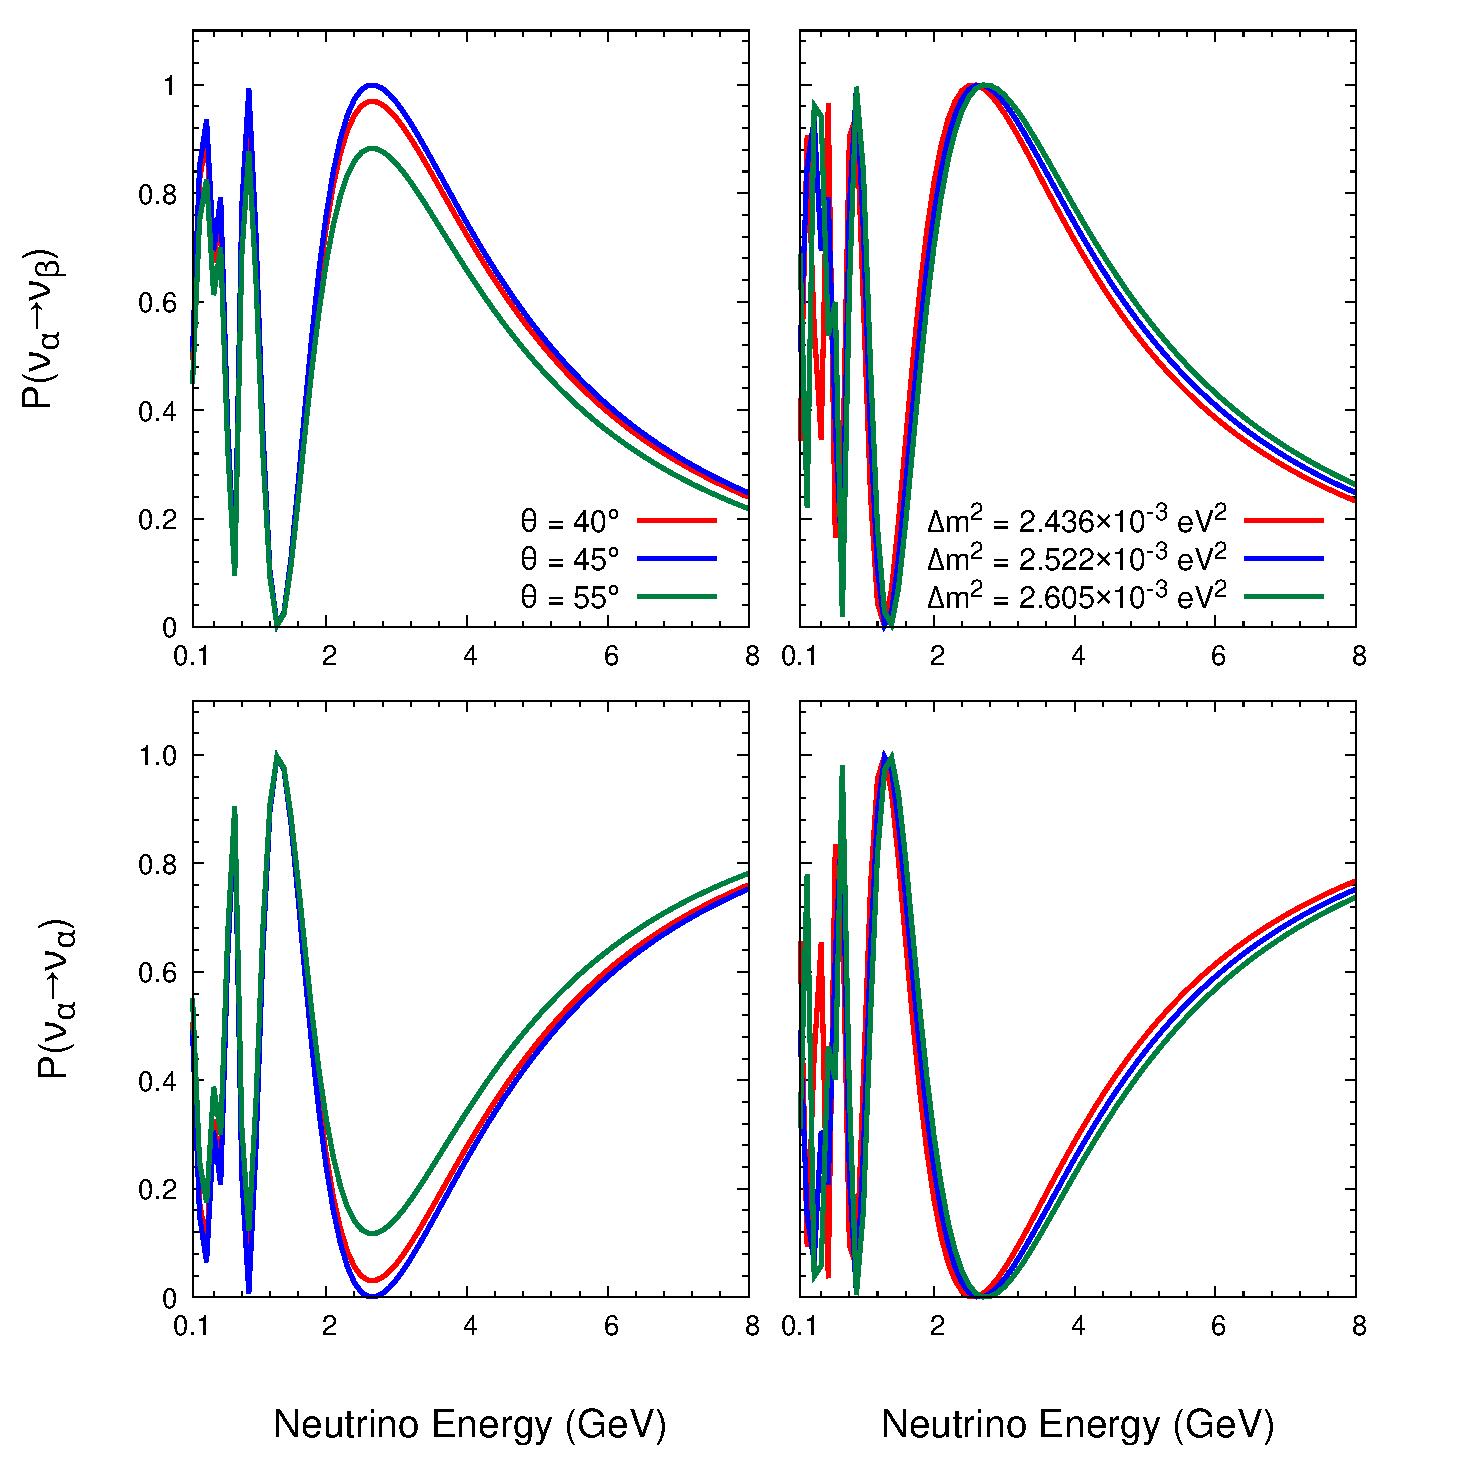
\includegraphics[width=\linewidth]{./Figures/Chapter-2/Thesis_multiplot_prob_app_disapp.pdf}	
    \caption{\footnotesize{Neutrino oscillation probability in vacuum at two flavor case as the function of true neutrino energy (in GeV) is depicted here. The upper (lower) panel represents $\nu_\alpha\rightarrow\nu_\beta$ appearance ($\nu_\alpha\rightarrow\nu_\alpha$ disappearance) probability using Equation \ref{eq:2 flavor app oscillation probability}. In the left panel, we observe the oscillation probability for three choices of mixing angle $\theta\,\,i.e.,\,\,40^\circ,\,45^\circ,\,\mathrm{and}\,\,\, 55^\circ$ (shown in red, blue, and green lines), respectively, assuming $L= 1300$ km and $\Delta m^2=+2.522\times10^{-3}$ eV$^2$. In the right panel, we compute the same but for three different choices of $\Delta m^2,\,\,i.e.,\,2.436\times10^{-3}$ eV$^2,\, 2.522\times10^{-3}$ eV$^2, \mathrm{and}\,\,\, 2.605\times10^{-3}$ eV$^2$ (shown by red, blue, and green lines), respectively, assuming a given mixing angle $\theta=45^\circ$.}}
	\label{fig:oscillation_prob_vacuum_analytical}
\end{figure} 
%------------------------------------
 \par Equation \ref{eq:2 flavor app oscillation probability} resembles with the standard oscillation formula in the acoustic medium, where the first part signifies the amplitude part (governed by the mixing angle $\theta$), whereas the second part depicts the frequency part (governed by the mass-squared difference $\Delta m^2$). If $\theta$ becomes $45^\circ$, appearance probability (\ref{eq:2 flavor app oscillation probability}) becomes maximum. Hence the value $\theta=45^\circ$ is called the maximal mixing (MM) value \cite{Xing:2015fdg}. Any other values of $\theta$ show lesser appearance probability than the maximal mixing for a given set of values of oscillation parameters. On the other hand, the shift of the frequency can be tuned to different energy and baseline lengths by controlling the value of $\Delta m^2$. 

 Figure~\ref{fig:oscillation_prob_vacuum_analytical} illustrates that the variations in the mixing angle enable precise modulation of the amplitude of the neutrino oscillation probability, while adjustments to the mass-squared difference primarily govern the phase shift of the oscillation pattern. The mixing angle $\theta$ signifies the extent of flavor mixing, with maximal mixing corresponding to the highest transition probability or the deepest suppression in survival probability. Moreover, in the oscillation frequency domain, an increase in the value of $\Delta m^2$ induces a phase shift toward higher neutrino energies, resulting in a rightward displacement of the oscillation peak.\\
 %-----------------------------------------------------
 \section{Formalism of neutrino oscillation probability in $3\nu$ paradigm}
 \label{sec:2.2}
 The discovery of the non-zero value of $\theta_{13}$ in the Daya Bay \cite{DayaBay:2012fng, DayaBay:2022orm} experiment connects the atmospheric neutrino sector and the solar neutrino sector, establishing the $3\nu$ paradigm on a strong footing. At the same time, the two-flavor neutrino oscillation delineates the values of the solar and atmospheric oscillation parameters, and the $3\nu$ paradigm with non-zero $\theta_{13}$ gives rise to the possibilities of observing CP violation in the neutrino sector. Now, we discuss the formalism of the three-flavor neutrino oscillation.
 \par Let, a neutrino of flavor $ \alpha$ is produced at $ x=0 $ with energy $E$, then the state of the neutrino at $x=0$ can be expressed as\\
 	\begin{align}
 		\ket{\nu_{\alpha}(x=0)}& =\nonumber\ket{\nu_\alpha}\\
 		&=\sum_{j=1}^{3}(U_{PMNS})^*_{\alpha j}\ket{\nu_j}.\\\nonumber
  	 	\end{align}
 At the position $x=L$, the neutrino state can be written as,\\
 \begin{align}
 	\ket{\nu_{\alpha}(x=L)}&=\nonumber\sum_{j=1}^{3}e^{ip_jL}(U_{PMNS})^*_{\alpha j}\ket{\nu_j}\\
 	&=e^{ip_kL}\sum_{j=1}^{3}e^{i(p_j-p_k)L}(U_{PMNS})^*_{\alpha j}\ket{\nu_j}.\\\nonumber
 \end{align}
   	
   	Assuming $m_j<<E$ we can approximate, \\
   	\begin{align}
   		p_j&=\nonumber\sqrt{E^2-m^2_j}\\
   		&=E-\frac{m^2_j}{2E}+...\\\nonumber.
   	\end{align}
   So,
   \begin{align}
   	p_j-p_k \approx -\frac{\Delta m^2_{jk}}{2E}\\\nonumber
   \end{align}
   where, $\Delta m^2_{jk}=m^2_j-m^2_k$ . \\
   	 %  	\newpage
   	   	Hence, we can write
   	   	\begin{align}
   	   		\ket{\nu_{\alpha}(x=L)}&=e^{ip_kL}\sum_{j=1}^{3}exp\left(-i\frac{\Delta m^2_{jk}\,L}{2E}\right)(U_{PMNS})^*_{\alpha j} \ket{\nu_j}.\\\nonumber
   	   	\end{align}
   	   	%\newpage
        \vspace{-1.5mm}
   	So, the probability amplitude of observing the neutrino flavor $\beta$ at $x=L$ is given by (neglecting the overall phase as it will be cancelled out while multiplying with its complex conjugate while obtaining the probability),   
	\begin{align}
  	\textrm{A}_{\beta\alpha}&=\nonumber\braket{{\nu_\beta}|\nu_{\alpha}(x=L)}\\\nonumber
	&=\nonumber\left[\sum_{k=1}^{3}\bra{\nu_k}(U_{PMNS})_{\beta k}\right]\left[\sum_{j=1}^{3}\exp\left(-i\frac{\Delta m^2_{jk}\,L}{2E}\right)(U_{PMNS})^*_{\alpha j}\ket{\nu_j}\right]\\\nonumber
   	&=\nonumber\sum_{j=1}^{3}(U_{PMNS})_{\beta j}\exp\left(-i\frac{\Delta m^2_{jk}\,L}{2E}\right)(U_{PMNS})^*_{\alpha j}\\
   	&=\sum_{j=1}^{3}U_{\beta j}\exp\left(-i\frac{\Delta m^2_{jk}\,L}{2E}\right)U^*_{\alpha j}.\\\nonumber
  	\end{align}	
  	So, the probability of oscillation from $\ket{\nu_\alpha}$ to $\ket{\nu_\beta}$ with true neutrino energy $E$ and baseline $L$ is given by,\\
  	\begin{align}
  		P(\nu_\alpha \rightarrow \nu_\beta)&=\nonumber|A_{\beta\alpha}|^2\\\nonumber
  		&=\nonumber|\sum_{j=1}^{3}U_{\beta j}exp\left(-i\frac{\Delta m^2_{jk}\,L}{2E}\right)U^*_{\alpha j}|^2\\\nonumber
  		&=\nonumber \left[\sum_{j=1}^{3}U_{\beta j}exp\left(-i\frac{\Delta m^2_{jk}\,L}{2E}\right)U^*_{\alpha j}\right]\times\left[\sum_{i=1}^{3}U_{\alpha i}exp\left(i\frac{\Delta m^2_{ik}\,L}{2E}\right)U^*_{\beta i}\right]\\
  		&=\sum_{j=1}^{3}\sum_{i=1}^{3}exp\left[-i\frac{\left(\Delta m^2_{jk}-\Delta m^2_{ik}\right)\,L}{2E}\right]\,U_{\beta j}U^*_{\alpha j}U_{\alpha i}U^*_{\beta i}\\\nonumber
  		\label{Equation 8}\\
  		&=\sum_{i}\sum_{j}\left(A_{ij}+iB_{ij}\right)\times\left(C_{ij}+iD_{ij}\right);    (say),\\\nonumber
  	\end{align}
   	   	where we assume, $exp\left[-i\dfrac{\left(\Delta m^2_{jk}-\Delta m^2_{ik}\right)\,L}{2E}\right]=A_{ij}+iB_{ij}$ and $U_{\beta j}U^*_{\alpha j}U_{\alpha i}U^*_{\beta i}=C_{ij}+iD_{ij}$. As the oscillation probability is a measurable quantity, so it should be real. Hence, we can drop the imaginary component of equation \ref{Equation 8}.\\
        
   	   	We break the sum of equation \ref{Equation 8} in two parts, $i.e.,$\\
   	   	\[
\sum_{i=1}^{3} \sum_{j=1}^{3} = \sum_{\substack{i=j=1}}^{3} + \sum_{\substack{i \neq j \\ i=1,\, j=1}}^{3}.
\]        
   	   	\textbf{\underline{Case - 1 :}}\\
   	   	for $i=j$,\\
   	  \begin{align}
   	  	 exp\left[-i\frac{\Delta m^2_{ii}\,L}{2E}\right]U_{\beta i}U^*_{\alpha i}U_{\alpha i}U^*_{\beta i}	&= U_{\beta i}U^*_{\alpha i}U_{\alpha i}U^*_{\beta i}.\\\nonumber
   	  \end{align}
   	   	\textbf{\underline{Case - 2 :}}\\
   	   for $i\neq j$,\\
   	   \begin{align}
   	   Re\left(exp\left[-i\frac{\Delta m^2_{ji}\,L}{2E}\right]\right)&=\nonumber \cos\left(\frac{\Delta m^2_{ji}\,L}{2E}\right)\\
   	   &=\cos(\Delta_{ji});\,\,(say, A_{ij}),\\
   	   Im\left(exp\left[-i\frac{\Delta m^2_{ji}\,L}{2E}\right]\right)&=\nonumber -\sin\left(\frac{\Delta m^2_{ji}\,L}{2E}\right)\\
   	   &=-\sin(\Delta_{ji});\,\,(say, B_{ij}).\\\nonumber
   	   \end{align}	
   	   	So, from equation \ref{Equation 8}, considering the real part only, we can write\\
   	   	\begin{align}
    P (\nu_\alpha \rightarrow \nu_\beta) &= A_{ij}C_{ij} - B_{ij}D_{ij} \nonumber \\
    &= Re (U^*_{\alpha i} U_{\beta i}U_{\alpha j}U^*_{\beta j}) 
    - 2\,Re (U^*_{\alpha i} U_{\beta i}U_{\alpha j}U^*_{\beta j}) \sin^2\left(\frac{\Delta_{ji}}{2}\right) \nonumber \\
    &\quad + Im\,(U^*_{\alpha i} U_{\beta i}U_{\alpha j}U^*_{\beta j}) \sin(\Delta_{ji}). \label{Equation12}
\end{align}
	   	Here, we have used $\cos(\Delta_{ji})=1-2\sin^2\left(\dfrac{\Delta_{ji}}{2}\right)$. So, taking case - 1 ($i.e.$, $i=j$) and case - 2 ($i\neq j$) together, we can write,
  \begin{align}
    P(\nu_\alpha \rightarrow \nu_\beta) &= \sum_{i}\sum_{j} \Big[ U_{\beta i}U^*_{\alpha i}U_{\alpha i}U^*_{\beta i} 
    + Re\,(U^*_{\alpha i} U_{\beta i}U_{\alpha j}U^*_{\beta j}) \nonumber \\
    &\quad - 2Re\,(U^*_{\alpha i} U_{\beta i}U_{\alpha j}U^*_{\beta j}) \sin^2\left(\frac{\Delta_{ji}}{2}\right) \nonumber \\
    &\quad + Im\,(U^*_{\alpha i} U_{\beta i}U_{\alpha j}U^*_{\beta j}) \sin(\Delta_{ji}) \Big]. \label{Equation}
\end{align}
  Now,
\begin{align}
    \left(\sum_{i=1}^{3}U^*_{\alpha i}U_{\beta i}\right)^2 &= 
    \left(U^*_{\alpha 1}U_{\beta 1} + U^*_{\alpha 2}U_{\beta 2} + U^*_{\alpha 3}U_{\beta 3} \right)^2 \nonumber \\
    &= \sum_{i}(U^*_{\alpha i}U_{\beta i})^2 + \sum_{i \neq j} 2(U^*_{\alpha i} U_{\beta i}U_{\alpha j}U^*_{\beta j}). \label{Equation13}
\end{align}
   So, from the equation \ref{Equation13}, we can write the final generalized form of the equation of neutrino oscillation probability in $3\nu$ framework as \\
   \begin{align}
    P(\nu_\alpha \rightarrow \nu_\beta) &= \delta_{\alpha\beta} 
    - 4\sum_{i>j} Re\,(U^*_{\alpha i} U_{\beta i}U_{\alpha j}U^*_{\beta j}) \sin^2\left(\frac{\Delta_{ji}}{2}\right) \nonumber \\
    &\quad + 2\sum_{i>j} Im\,(U^*_{\alpha i} U_{\beta i}U_{\alpha j}U^*_{\beta j}) \sin(\Delta_{ji}). \label{Equation14}
\end{align}
If $i$ and $j$ take only values from 1 to 2, the above equation reduces to the two-flavor neutrino oscillation expression. The third term of equation \ref{Equation14} represents the CP violation. The PMNS matrix can be written as,
\begin{equation}
   	  U= 
   	   \begin{pmatrix}
	1 & 0 & 0 \\
	0 & c_{23} & s_{23} \\
	0 & -s_{23} & c_{23}
\end{pmatrix} 
\begin{pmatrix}
	c_{13} & 0 & s_{13}e^{-i\delta} \\
	0 & 1 & 0 \\
	-s_{13}e^{i\delta} & 0 & c_{13}
\end{pmatrix}
\begin{pmatrix}
	c_{12} & s_{12} & 0 \\
	-s_{12} & c_{12} & 0 \\
	0 & 0 & 1
\end{pmatrix} \nonumber
   \end{equation}
   \begin{align}
   & =
   	\begin{pmatrix}
   	   {c_{12}c_{13}} & {s_{12}c_{13}} & {s_{13}e^{-i\delta}}\\
   	  {-s_{12}c_{23}-c_{12}s_{13}s_{23}e^{i\delta}} & {c_{12}c_{23}-s_{12}s_{13}s_{23}e^{i\delta}} & {c_{13}s_{23}}\\
   	   {s_{12}s_{23}-c_{12}s_{13}c_{23}e^{i\delta}} & {-c_{12}s_{23}-s_{12}s_{13}c_{23}e^{i\delta}} & {c_{13}c_{23}}
   	   \end{pmatrix}
       \label{PMNS matrix}
   \end{align}
   \begin{align}
   & \equiv
   	\begin{pmatrix}
   	U_{\alpha 1} & U_{\alpha 2} & U_{\alpha 3}\\
   	U_{\beta 1} & U_{\beta 2} & U_{\beta 3}\\
   	U_{\gamma 1} & U_{\gamma 2} & U_{\gamma 3}
   	\end{pmatrix}.
   \end{align}
 Here, $c_{ij}$ and $s_{ij}$ stand for $\cos\theta_{ij}$ and $\sin\theta_{ij}$, respectively, where $i,j= 1,2,3; \,\,i\neq j$. We are ignoring the Majorana phases here as they do not affect the neutrino oscillation probability. The advantage of considering the PMNS matrix as a suitable unitary mixing matrix connecting the flavor basis and mass basis of neutrinos is that the ratios of some matrix elements of $U$ give us the values of the oscillation parameters distinctly. For example,\\
 \begin{equation}
     \tan^2\theta_{23} = \frac{|U_{\beta3}|^2}{|U_{\gamma3}|^2}, \\\nonumber
 \end{equation}
 and,  \begin{equation}
     \tan^2\theta_{12} = \frac{|U_{\alpha2}|^2}{|U_{\alpha1}|^2} \\\nonumber.
 \end{equation}
The 1-3 element of the PMNS matrix gives us the value of $\delta_{\mathrm{CP}}$ if the value of $\theta_{13}$ is well known. The ratios of other matrix elements of $U$ also give the value of the oscillation parameters, $e.g.$, 
\ \begin{equation}
     \cos^2\theta_{12} = \frac{\left| U_{\alpha1} \right|^2}{ 1 - \left|U_{\alpha3} \right|^2} \nonumber,\,\,\sin^2\theta_{12} = \frac{\left| U_{\alpha2} \right|^2}{ 1 - \left|U_{\alpha3} \right|^2} \nonumber, \\
   \cos^2\theta_{23} = \frac{\left| U_{\gamma3} \right|^2}{ 1 - \left|U_{\alpha3} \right|^2} \nonumber,\,\,\sin^2\theta_{23} = \frac{\left| U_{\beta3} \right|^2}{ 1 - \left|U_{\alpha3} \right|^2}. \nonumber \\  
\end{equation}
Now, substituting the values of the matrix elements from equation \ref{PMNS matrix} to equation \ref{Equation14}, we get the final expression of neutrino oscillation probability in vacuum. If we focus on appearance channels only ($i.e.,\, \alpha \neq \beta$ in equation \ref{Equation14}) and keep the terms upto second order of ($\alpha\cdot\sin(2\theta_{13})$), where $\alpha=\dfrac{\Delta m^2_{21}}{\Delta m^2_{31}}$, then equation \ref{Equation14} takes the following form \cite{Akhmedov:2004ny}.\\

\begin{align}
    P(\nu_{\mu} \rightarrow \nu_{e}) \simeq 
    &\ \bm{\sin^2\theta_{23}} \sin^2(2\theta_{13}) 
    \sin^2\Delta \nonumber \\
    &+ (\alpha\Delta) \sin(2\theta_{13})\sin(2\theta_{12})\sin(2\theta_{23}) \bm{\sin (\delta_{\mathrm{CP}})} \sin^2(\Delta) \nonumber \\
    &+ (\alpha\Delta) \sin(2\theta_{13})\sin(2\theta_{12})\sin(2\theta_{23}) \bm{\cos( \delta_{\mathrm{CP}})} \cos(\Delta)\sin(\Delta) \nonumber \\
    &+ (\alpha\Delta)^2 \cos^2\theta_{23} \sin^2(2\theta_{12}).
    \label{Four_term_app_prob}
\end{align}
\par The first term in the equation \ref{Four_term_app_prob} is the leading term as it does not depend on $\alpha$ (as $\alpha<<1$) and governed by the atmospheric mixing angle $\theta_{23}$. Here, $\Delta=\dfrac{\Delta m^2_{31}\,L}{4E}$. Note that, this term depends on $\sin^2\theta_{23}$ and sensitive to the octant of $\theta_{23}$, hence the $\nu_\mu\rightarrow\nu_e$ appearance channel helps to resolve the octant of $\theta_{23}$. Although, there is a sub-leading effect of the second term, it gives the signature of CP violation as $\sin(\delta_{\mathrm{CP}})$ changes sign as $\delta_{\mathrm{CP}}$ changes its sign when we go from neutrino to antineutrino, $i.e.,$ it is a CP-odd term. Hence, the $\nu_\mu\rightarrow\nu_e$ appearance channel helps to study CP violation (Dirac $\bm{\delta_{\mathrm{CP}}}$) in the neutrino sector. The third term is the CP-even term. The last term is the solar term and depends on the solar mixing angle $\theta_{12}$. But, its contribution in the appearance channel is very much suppressed due to its $\alpha^2$ dependence.\\
\par Similarly, we can study some features of the $\nu_\mu\rightarrow\nu_\mu$ disappearance probability in vacuum by writing its expression following the previous approximations,
\begin{align}
    P(\nu_{\mu} \rightarrow \nu_{\mu}) \simeq 
    &\ 1- \bm{\sin^22\theta_{23}} \sin^2(\Delta) \nonumber \\
    &+ 4\sin^2\theta_{13}\sin^2\theta_{23}\cos(2\theta_{23})\sin^2\Delta \nonumber\\
    &+ (\alpha\Delta) \sin2\Delta [\cos^2\theta_{12}\sin^22\theta_{23}-2\sin\theta_{13}\sin2\theta_{12}\sin^2\theta_{23}\sin2\theta_{23}\bm{\cos\delta_{\mathrm{CP}}}] \nonumber \\
    &- (\alpha\Delta)^2 [\sin^22\theta_{12}\cos^2\theta_{23}+\cos^2\theta_{12}\sin^22\theta_{23}(\cos2\Delta-\sin^2\theta_{12})].
    \label{Four_term_disapp_prob}
\end{align}
The first salient feature of the above expression is that the leading term is proportional to $\sin^22\theta_{23}$ and therefore it is not sensitive to the octant of $\theta_{23}$, but its strength is larger than the $\nu_\mu\rightarrow\nu_e$ appearance probability in equation \ref{Four_term_app_prob}, which is suppressed by $\sin^2(2\theta_{13})$. Hence, the disappearance channel is rich in statistics. Furthermore, this channel is not sensitive to the CP violation as it only contains $\cos\delta_{\mathrm{CP}}$ term. The motivations behind showcasing only these two channels throughout this thesis are i) the $\nu_\mu\rightarrow\nu_e$ appearance channel \cite{Huber:2002mx, Cervera:2000kp} is sensitive to two of the most important unresolved issues in the $3\nu$ paradigm, $i.e.,$ CP violation and exclusion of the wrong octant solution of $\theta_{23}$, ii) the $\nu_\mu\rightarrow\nu_\mu$ disappearance channel ensures to bring good precision in measuring the atmospheric oscillation parameters $\theta_{23}$ and $\Delta m^2_{31}$ owing to high statistics in this channel in long-baseline (LBL) experiments (for details, see the next chapter on long-baseline experiments). For antineutrinos, the sign of $\delta_{\mathrm{CP}}$ changes its sign ($i.e., P(\nu_\alpha\rightarrow\nu_\beta;\,\delta_{\mathrm{CP}})\rightarrow P(\bar{\nu}_\alpha\rightarrow\bar{\nu}_\beta;\,-\delta_{\mathrm{CP}})$).
\par The CP-odd asymmetry in neutrino oscillation can be written as,
\begin{align}
    \Delta P_{\alpha \beta} &= P(\nu_\alpha\rightarrow\nu_\beta) - P(\bar{\nu}_\alpha\rightarrow\bar{\nu}_\beta) \nonumber\\
    &= \pm 16J\sin\left(\frac{\Delta m^2_{21}L}{4E}\right) \sin\left(\frac{\Delta m^2_{31}L}{4E}\right) \sin\left(\frac{\Delta m^2_{32}L}{4E}\right).
    \label{Delta P}
\end{align}
Here, $\Delta P_{\alpha \beta}$ denotes the amount of CP-odd asymmetry in the neutrino sector, $J$ is the Jarlskog invariant ($J\equiv Im[U_{e1}U^*_{\mu 1}U^*_{e 2}U_{\mu 2}]$) \cite{Jarlskog:1985ht, Jarlskog:1985cw}, which is a constant quantity irrespective of the choice of basis, and can be expressed under the standard PMNS parameterization as,
\begin{equation}
    J = \frac{1}{8} \cos\theta_{13} \sin (2\theta_{12}) \sin (2\theta_{13}) \sin (2\theta_{23}) \sin \delta_{\mathrm{CP}}.\\
    \label{Jarlskog invariant}
\end{equation}
Equations \ref{Delta P} and \ref{Jarlskog invariant} denote the necessary conditions for CP violation in the neutrino sector \cite{Antusch:2001ck}, $i.e.,$%
\begin{itemize}[topsep=-0.5pt, itemsep=10pt, parsep=0pt, partopsep=0pt]
    \item the mixing angles $\neq 0^\circ, \, 90^\circ,$
    \item the value of $\delta_{\mathrm{CP}} \neq 0^\circ, \pm 180^\circ$,
    \item the value of $\Delta m^2_{ij} \neq 0$.
\end{itemize}




%%%%%%%%%%%%%%%%%%%%%%%%%%%%%%%%%%%%%%%%%%%%%%%%%%%%%%%%%%%%%%%%%%%%%%%%%%%%%%%%%%%%%%%%%%%%%%%%%%%%%%%%%%%%%%%%%%%%%%%%%%%%%%%%%%%%%%%%%%%%%%%%%%%%%%%%%%%%%%%%%%%%%%%%%%%%
\section{Manifestation of matter effect in neutrino oscillation}
\label{sec:2.3}
Neutrinos interact with the ambient matter via weak interactions and it can modify the oscillation probabilities of neutrinos. The first experimental evidence of matter effects in neutrino oscillations came from the solar neutrino experiments, particularly the Sudbury Neutrino Observatory (SNO) \cite{SNO:2002hgz} and Super-Kamiokande \cite{Super-Kamiokande:2013mie}, around the early 2000s. These experiments confirmed the Mikheyev-Smirnov-Wolfenstein (MSW) effect \cite{Wolfenstein:1977ue, Mikheyev:1989dy, Mikheyev:1985zog}, which describes how the oscillation probability of neutrinos gets modified as they travel through dense matter.
\par The modified Hamiltonian incorporating the neutrino-matter interaction can be written as,
\begin{equation}
    \hat{H}_{eff} = \hat{H}_{vac}+ \hat{H}_{matt}.
    \label{eq:general hamiltonian matter effect}
\end{equation}
To have a close look at how the eigenvalues are modified under the influence of the neutrino-matter interaction, we take the help of the time-dependent Schr\"{o}dinger equation, $i.e.,$
\begin{equation}
    i \frac{d}{dt} \ket{\nu(t)} = \hat{H}_{eff} \ket{\nu(t)}.
    \label{Schrodinger eqn}
\end{equation}
This equation \ref{Schrodinger eqn} can be rewritten in the flavor eigenstate as,
\begin{equation}
    i \frac{d}{dt} \nu_{\alpha} (t) = \sum_{\beta} H_{\alpha\beta} \nu_{\beta} (t),
\end{equation}
where $\alpha,\beta$ denote the flavor indices and $H_{\alpha\beta}= \langle \nu_\alpha | H | \nu_\beta \rangle$ are the matrix elements. On the other hand, $\ket{\nu_k}$ denotes the mass eigenstate and hence the eigenstate of the free Hamiltonian $\hat{H}_{vac},\, i.e.,$
\begin{equation}
\hat{H}_{vac} \ket{\nu_k} = E_k\ket{\nu_k},
\label{vacuum equation}
\end{equation}
where, $E_k$ denotes the eigenvalue of the free Hamiltonian and can be written as $E_k=\sqrt{\vec{p}^2+m^2_k}$, $\vec{p}$ being the momentum of the mass eigenstate $\ket{\nu_k}$. Neutrinos interact with the electrons of the ordinary matter through charged-current (CC) interaction via the $W^\pm$ boson of the SM. This interaction induces a matter potential confronting which the neutrino changes its flavor while propagating through a medium. This potential can be depicted as,
\begin{align}
    V_{CC,\alpha} &= \sqrt{2} G_F N_e, \quad [\alpha = e] \\\nonumber
    &= 0, \quad [\alpha = \mu,\tau].
    \label{eq:V_cc}
\end{align}
Neutrinos mainly interact with the ambient electron of the matter while performing charged current interaction. There is another kind of interaction of neutrinos with the matter via the neutral mediator $Z^0$ boson of the SM, hence it is called neutral current (NC) interaction \cite{Linder:2005fc}, the matter potential of which can be expressed as,
\begin{align}
    V_{NC,\alpha} &= -\frac{G_F}{\sqrt{2}} N_n, \quad [\alpha = e, \mu, \tau], \\\nonumber,
\end{align}
where, $N_e$ and $N_n$ signify the electron number and neutron number densities of the matter, and $G_F$ denotes the Fermi coupling constant 
 ($G_F=1.166\times10^{-5}$ GeV$^{-2}$). Neutrinos interact with the matter via coherent and forward scattering \cite{COHERENT:2020iec}. Due to the scarcity of naturally produced muon and tau in the Earth matter, CC interaction only occurs with the electrons of the medium. Now, the CC interaction potential can be expressed in terms of some measurable parameters used in the experiments directly, $i.e.,$ line-averaged Earth matter density  $\rho_{\text{avg}}$ \cite{Kelly:2018kmb} and the above-mentioned number densities ($i.e., N_e \,\mathrm{and}\, N_n$) as the following fashion,
 \begin{equation}
     V_{CC}\approx 7.6\times\left(\frac{N_e}{N_p+N_n}\right)\times\left[\frac{\rho_{\text{avg}}}{10^{14} \,\mathrm{g/cm^{3}}}\right] \mathrm{eV}.
     \label{CC matter pot}
 \end{equation}
Considering further the medium of interaction is electrically neutral ($i.e., N_e=N_p$) and isoscaler ($i.e., N_p=N_n$), equation \ref{CC matter pot} can be rewritten as,
\begin{equation}
    V_{CC} = 7.6 \times 0.5 \times\left[\frac{\rho_{\text{avg}}}{10^{14}\, \mathrm{g/ cm^{3}}}\right] \mathrm{eV}.
\end{equation}
The total matter potential $V(\nu)_\alpha = V_{CC,\alpha}+V_{NC,\alpha}$ changes its polarity while considering antineutrinos instead of neutrinos $i.e., V(\nu)_\alpha = -V(\bar{\nu})_\alpha $. This $V_\alpha$ is the eigenvalue of the Hamiltonian $\hat{H}_{\mathrm{matt}}$ in weak basis, $i.e.,$
\begin{equation}
    \hat{H}_{\mathrm{matt}}\ket{\nu_\alpha}= V_\alpha\ket{\nu_\alpha}.
\end{equation}
 At tree level, neutral-current interactions mediated by the $Z^0$ boson are flavour universal, giving identical contributions to all active neutrinos, and hence it does not affect the oscillation probability. However, at the one-loop level, radiative corrections to the neutrino--$Z^0$ vertex involve virtual $W$ bosons and the corresponding charged lepton partner. Since these corrections depend on the charged lepton mass, the large difference between $m_\mu$ and $m_\tau$ breaks flavor universality, leading to a small but finite splitting between the effective matter potentials of $\nu_\mu$ and $\nu_\tau$~\cite{Botella:1986wy}. The difference between the matter potential confronted by $\nu_\mu$ and $\nu_\tau$ can be written as \cite{Mirizzi:2009td},
	\begin{align}
		\Delta V_{\tau\mu}=V_\tau-V_\mu=-\dfrac{3\sqrt{2}}{2\pi^2}G_Fm^2_\tau\bigg(ln \dfrac{m_W}{m_\tau} -\dfrac{1}{2}\bigg)\dfrac{N_e}{m^2_W},
		\label{eq:Higher_MSW_analysis}
	\end{align}
	where, $m_\tau$ and $m_W$ denote mass of tau and $W$ boson. For Earth matter, the relative contribution of this splitting with respect to the potential $V_{\text{CC,e}}$ is
	\begin{align}
		\dfrac{\Delta V_{\tau\mu}}{V_{\text{CC,e}}}\sim -2.5\times10^{-4}.
	\end{align}
	Although in standard interaction of active neutrinos, this effect is negligible, but from the context of dense environments like supernova, this slight difference between the interaction potentials becomes significant. It is the first non-zero splitting for the NC interaction of $\nu_\mu$ and $\nu_\tau$ (or in the 2-3 sector) which could affect neutrino oscillation in dense media.
	
 From equation \ref{vacuum equation}, it is evident that the energy of the neutrinos is the eigenvalues of the vacuum Hamiltonian in mass basis. To convert it into the physically measurable flavor basis, we need to diagonalize it through the unitary mixing matrix $U$ by the following equation
\begin{equation}
    \hat{H}^f_{vac}= U\hat{H}^m_{vac}U^\dagger.
\end{equation}. 
In the matrix form, it can be written as,
\begin{equation}
    H^f = \mathbf{U}
    \begin{bmatrix}
        E_1^m & 0 & 0 \\
        0 & E_2^m & 0 \\
        0 & 0 & E_3^m
    \end{bmatrix}
    \mathbf{U}^\dagger.
\end{equation}
After invoking the influence of the matter effect in our picture, this mixing matrix $U$ cannot diagonalize the effective Hamiltonian $\hat{H}_{eff}$, and it will not be diagonal even on the previous mass basis, considered so far. Hence, we need to construct a new type of mass basis (say, $\ket{\nu^m_i}$) where $\hat{H}_{vac}$ is diagonal. In this matter-modified mass basis $\ket{\nu^m_i}$, the diagonalized form of the effective Hamiltonian will be $\hat{H}^m=diag\, (E^m_1, E^m_2, E^m_3)= diag\, \frac{1}{2E}(\Tilde{m}^2_1, \Tilde{m}^2_2, \Tilde{m}^3_3)=\Tilde{U}\hat{H}_{eff} \Tilde{U}^\dagger$. Here, $\Tilde{U}$ is the matter-modified mixing matrix (kindly note that, $\ket{\nu^m_i}\neq\ket{\nu_i},\,\Tilde{U}^m\neq U$). Like the previous case, here also we assume equal momentum approximation ($i.e., E_1=E_2=E_3=E$) and $\Tilde{m}^2_i$ signifies the matter-modified mass squared term. So, the flavor basis can now be expressed in terms of the matter-modified mass basis through this relation $\ket{\nu_\alpha}=\Tilde{U}\ket{\nu^m_i}$. Adorned with this new mass basis and new mixing matrix, we can show the neutrino oscillation probability while neutrinos interact through matter with the two new plug-ins, $U_{\alpha i}\rightarrow \Tilde{U}^m_{\alpha i}$ and $E_i\rightarrow E^m_i$, where $E^m_i$ is the matter-modified energy eigenvalue of each mass state. Now, following the footprints of the same calculations mentioned in the section \ref{sec:2.2}, we can write down the expression of the neutrino oscillation probability under the influence of the matter effect as,
\begin{align}
    P(\nu_\alpha \rightarrow \nu_\beta) &= \delta_{\alpha\beta} 
    - 4\sum_{i>j} Re (\Tilde{U}^*_{\alpha i} \Tilde{U}_{\beta i}\Tilde{U}_{\alpha j}\Tilde{U}^*_{\beta j}) \sin^2\left(\frac{\Tilde{\Delta}_{ji}}{2}\right) \nonumber \\
    &\quad + 2\sum_{i>j} Im (\Tilde{U}^*_{\alpha i} \Tilde{U}_{\beta i}\Tilde{U}_{\alpha j}\Tilde{U}^*_{\beta j}) \sin(\Tilde{\Delta}_{ji}), \label{eq: matt modified oscillation probability}
\end{align}
where, $\Tilde{\Delta}_{ji} = \dfrac{\Delta\Tilde{m}^2_{ji}L}{4E}$ denotes the modified frequency term with two measurable quantities, baseline length ($L$ in km) and the neutrino energy ($E$ in GeV).
%---------------------------------------------------------


\subsection{Overview of the matter effect in two-flavor neutrino oscillation}
To understand the influences of the matter effect on the neutrino oscillation and the modifications of its expression, we consider the simple two-flavor oscillation first. Following the equation \ref{eq:general hamiltonian matter effect} and \ref{eq:V_cc}, we can rewrite the effective Hamiltonian in the matrix form as,
\begin{align}
\label{eq:2 flavor matter effect}
    \hat{H}_{\text{eff}} &= \mathbf{U}
    \begin{bmatrix}
         0 & 0 \\
         0 & \dfrac{\Delta m^2}{2E}
    \end{bmatrix}
    \mathbf{U}^\dagger
    + \begin{bmatrix}
         V_{CC} & 0 \\
         0 & 0
    \end{bmatrix} \\
    &= \begin{bmatrix}
         \cos\theta & \sin\theta \\
         -\sin\theta & \cos\theta
    \end{bmatrix}
    \begin{bmatrix}
         0 & 0 \\
         0 & \dfrac{\Delta m^2}{2E}
    \end{bmatrix}
    \begin{bmatrix}
         \cos\theta & -\sin\theta \\
         \sin\theta & \cos\theta
    \end{bmatrix}
    + \begin{bmatrix}
         V_{CC} & 0 \\
         0 & 0
    \end{bmatrix} \nonumber \\
    &= \dfrac{\Delta m^2}{4E}
    \begin{bmatrix}
         \left(1-\cos2\theta+\dfrac{4EV_{CC}}{\Delta m^2}\right) & \sin2\theta \\
         \sin2\theta & 1+\cos2\theta
    \end{bmatrix}. \nonumber
\end{align}
If we diagonalize the matrix mentioned in \ref{eq:2 flavor matter effect}, then the eigenvalues are,
\begin{align}
    E^m_1=\frac{V_{CC}}{2}+\frac{\Delta m^2}{4E} \left[1-\sqrt{\sin^22\theta+\left(\cos2\theta-\frac{2EV_{CC}}{\Delta m^2}\right)^2}\right]\\
   E^m_2=\frac{V_{CC}}{2}+\frac{\Delta m^2}{4E} \left[1+\sqrt{\sin^22\theta+\left(\cos2\theta-\frac{2EV_{CC}}{\Delta m^2}\right)^2}\right]\nonumber.
\end{align}
Now, we can parameterize the modified mixing matrix $\Tilde{U}^m$ with the matter-modified oscillation parameter $\theta^m$ and write the form of $\Tilde{U}^m$ as,
\begin{align}
    U^m &= 
    \begin{bmatrix}
         \cos\theta^m & \sin\theta^m \\
         -\sin\theta^m & \cos\theta^m
    \end{bmatrix}.
    \end{align}
The link between the matter-modified oscillation parameter ($\theta^m$) and the same in vacuum can be expressed as,
\begin{equation}
    \sin2\theta^m=\frac{\sin2\theta}{\sqrt{\sin^22\theta+\left[\cos2\theta-\dfrac{2EV_{CC}}{\Delta m^2}\right]^2}}.
    \label{resonance condition}
\end{equation}
If, in the denominator of the equation \ref{resonance condition}, $\cos2\theta=\dfrac{2EV_{CC}}{\Delta m^2}$ , $\theta^m$ will be $45^\circ$ (maximal mixing value). This phenomenon is called ``MSW (Mikhev-Smirnov-Wolfenstein) resonance" \cite{Smirnov:2019kto}, and the expression $\cos2\theta=\dfrac{2EV_{CC}}{\Delta m^2}$ is the criterion of this resonance. Neutrinos can show the MSW resonance if $\Delta m^2>0$, whereas antineutrinos can show it when $\Delta m^2<0$, as $V_{CC}$ changes its polarity for antineutrinos. 
\par Now, following the recipes used to derive the equation \ref{eq:2 flavor oscillation probability}, the revised expression of the probability of neutrino oscillation from a flavor $\alpha$ to a flavor $\beta$ is,
\begin{align}
P(\nu_{\alpha} \rightarrow \nu_{\beta}) &= \sin^2(2\theta^m) \sin^2\left( 1.27 \times \frac{\Delta \Tilde{m}^{2} L}{E} \right) \\
&= \sin^2(2\theta^m) \sin^2\left[\frac{\Delta m^2 L}{4E}\sqrt{\sin^22\theta+\left(\cos2\theta-\frac{2EV_{\mathrm{CC}}}{\Delta m^2}\right)^2}    \right].
\label{eq:2 flavor oscillation probability matter}
\end{align}
\par Some key takeaways from the equation \ref{eq:2 flavor oscillation probability matter} are,
\begin{itemize}
    \item If we change the polarity of $\Delta m^2$, the oscillation probability is affected due to the change of the $\theta^m$ and $\Delta \Tilde{m}^2$. So, the matter effect is a good portal to investigate the correct mass hierarchy in Nature.
    \item If we consider the extreme values of the matter potential V, then for $V=0$, the equation \ref{eq:2 flavor oscillation probability matter} reduces to the equation \ref{eq:2 flavor oscillation probability}. On the other hand, if $V\rightarrow \infty$, then the oscillation probability vanishes due to the lack of oscillation in the presence of an infinitely dense medium.
    \item Non-degenerate value of $m^2$ is crucially required for the neutrino oscillation either in vacuum or in matter.   
\end{itemize}

\subsection{The influence of matter effect in $3\nu$ framework}
By advancing our next step to the experimentally confirmed three-flavor case, we just expand the matrix form of the Hamiltonian [from equation \ref{eq:general hamiltonian matter effect}] in $3\times3$ dimension by introducing one additional mass-squared splitting, $i.e.$, atmospheric mass-splitting ($\Delta m^2_{31}$). The form of the effective Hamiltonian introducing matter effect in three flavors \cite{Agarwalla:2021zfr} is,
\begin{align}
    \hat{H}_{\text{eff}} &= \mathbf{U}
    \begin{bmatrix}
         0 & 0 & 0\\
         0 & \dfrac{\Delta m^2_{21}}{2E} & 0\\
         0 & 0 & \dfrac{\Delta m^2_{31}}{2E}
    \end{bmatrix}
    \mathbf{U}^\dagger
    + \begin{bmatrix}
         V_{CC} & 0 & 0\\
         0 & 0 & 0\\
         0 & 0 & 0\\
    \end{bmatrix}. 
    \label{eq:3 flavor matter effect}
\end{align}
Note that, here, $U$ is the ($3\times3$) unitary mixing matrix and is considered as the usual PMNS matrix for convenience. Now, we have to follow the same way we show in the previous section. But, to construct a new basis where the matter-modified Hamiltonian will be diagonalized in $3\nu$ framework is a bit tideous job. However, after diagonalizing the Hamiltonian, we land up to the following expression of matter-modified neutrino oscillation probability in $\nu_\mu\rightarrow\nu_e$ appearance channel by taking the approximation of considering only upto the 2nd order of ($\alpha\cdot\sin(2\theta_{13})$) \cite{Akhmedov:2004ny}.
\begin{align}
    P(\nu_{\mu} \rightarrow \nu_{e}) \simeq 
    &\ \bm{\sin^2\theta_{23}} \sin^2(2\theta_{13}) 
   \frac{\sin^2[(A-1)\Delta]}{(A-1)^2} \nonumber \\
    &+ \alpha \sin(2\theta_{13})\sin(2\theta_{12})\sin(2\theta_{23}) \bm{\sin (\delta_{\mathrm{CP}})} \sin(\Delta) \frac{\sin(A\Delta)}{A} \bm{\frac{\sin[(A-1)\Delta]}{(A-1)}}\nonumber \\
    &+ \alpha \sin(2\theta_{13})\sin(2\theta_{12})\sin(2\theta_{23}) \cos (\delta_{\mathrm{CP}}) \cos(\Delta) \frac{\sin(A\Delta)}{A} \frac{\sin[(A-1)\Delta]}{(A-1)} \nonumber \\
    &+ \alpha^2 \cos^2\theta_{23} \sin^2(2\theta_{12}) \frac{\sin^2(A\Delta)}{A^2},
    \label{Four_term_app_prob_matter}
\end{align}
where, $A=\pm\dfrac{2\sqrt{2}G_FN_eE}{\Delta m^2_{31}}$ stands for the dimensionless normalized matter potential [positive (negative) sign is for neutrino (antineutrino)] and $\Delta = \dfrac{\Delta m^2_{31}L}{4E}$. 
The same characteristic features of this equation through $\nu_\mu\rightarrow\nu_e$ appearance channel mentioned in \ref{Four_term_app_prob} hold good in the equation \ref{Four_term_app_prob_matter} also. Additionally, we highlight one more fact crucially contributed only by the matter effect in this channel. In the second term ($i.e.$, CP-violating term) of equation \ref{Four_term_app_prob_matter}, if we consider the interactions of antineutrinos with the matter, then the sign of the matter potential will be changed, \textit{i.e.,} $A\rightarrow -A $ and $\delta_{\mathrm{CP}}\rightarrow -\delta_{\mathrm{CP}}$. Consequently, the value of the term $\dfrac{\sin[(A-1)\Delta]}{(A-1)}$ will be changed. If the value of $\delta_{\mathrm{CP}}$ becomes zero, the matter term $\dfrac{\sin[(A-1)\Delta]}{(A-1)}$ will still affect the value of the appearance probability, producing a matter-induced (fake) CP violation. In this case, even if we do not consider the change of the sign of intrinsic $\delta_{\mathrm{CP}}$ ($i.e.,\,\sin(\delta_{\mathrm{CP}})$), the value of the last term ($i.e.,\,\dfrac{\sin[(A-1)\Delta]}{(A-1)}$) will be changed.\\ Thus, it is difficult to understand if the value of appearance probability changes due to intrinsic $\delta_{\mathrm{CP}}\,(i.e., \sin(\delta_{\mathrm{CP}}))$ term or due to the contribution of matter effect ($i.e., \dfrac{\sin[(A-1)\Delta]}{(A-1)}$). Therefore, the matter effect mimics a CP-violating signal in this channel, creating ambiguity in identifying whether the observed change in appearance probability originates from intrinsic $\delta_{\mathrm{CP}}$ or from matter-induced effects. This confusion is enhanced if the strength of the matter potential ($A$) becomes relatively high due to the higher line-averaged density of the Earth matter. Hence, we focus on an important point from the above expression. The $\nu_\mu\rightarrow\nu_e$ appearance channel is contaminated with fake CP violation \cite{deGouvea:2016pom, Agarwalla:2022xdo}. The amount of contamination increases with the increment of the value of the line-averaged Earth matter density. So, this channel solely is not a good probe to measure the intrinsic $\delta_{\mathrm{CP}}$ in Nature. 
\par Similarly for the $\nu_\mu\rightarrow\nu_\mu$ disappearance channel, we can write the oscillation probability under the influence of matter effect as,
\begin{samepage}
\begin{flalign}
     P(\nu_\mu \to \nu_\mu) \nonumber\\
    &= 1 - \sin^2 2\theta_{23} \sin^2 \Delta  - 4 s_{13}^2 s_{23}^2 \frac{\sin^2 (A-1)\Delta}{(A-1)^2}\nonumber \\
    &+ \alpha^2 \sin^2 2\theta_{12} c_{23}^2 \frac{\sin^2 A \Delta}{A^2} - (\alpha \Delta)^2 c_{12}^4 \sin^2 2\theta_{23} \cos 2\Delta  \nonumber \\
    &+ \frac{1}{2A} \alpha^2 \sin^2 2\theta_{12} \sin^2 2\theta_{23} \left( \sin \frac{\sin A \Delta}{A} \cos (A-1)\Delta - \frac{\Delta}{2} \sin 2\Delta \right) \nonumber \\
    &- \frac{2}{A-1} s_{13}^2 \sin^2 2\theta_{23} \left( \sin A \Delta \cos A \Delta \frac{\sin (A-1)\Delta}{(A-1)} - \frac{A\Delta}{2} \sin 2\Delta \right) \nonumber \\
    &- 2\alpha s_{13} \sin 2\theta_{12} \sin 2\theta_{23} \cos \delta_{\text{CP}} \cos \Delta \frac{\sin A \Delta}{A} \frac{\sin (A-1)\Delta}{(A-1)} \nonumber \\
    &+ \frac{1}{A-1} \alpha s_{13} \sin 2\theta_{12} \sin 4\theta_{23}\bm{\cos \delta_{\text{CP}}} \sin \Delta\left[A \sin \Delta - \frac{\sin A \Delta}{A} \cos (A-1)\Delta)\right], &&
    \label{eq:disapp oscillation prob matter}
\end{flalign}
\end{samepage}
where, $c_{ij}\, (s_{ij})$ stands for $\cos\theta_{ij}\,(\sin\theta_{ij})$. The polarities of $A$ and intrinsic $\delta_{\mathrm{CP}}$ are changed if we switch from neutrino to antineutrino. Similarly, considering neutrinos also, if we shift from the normal mass ordering (NMO, \textit{i.e.,} $\Delta m^2_{31}>0$) to the inverted mass ordering (IMO, \textit{i.e.,} $\Delta m^2_{31}<0$), there will be a sign flip of $A$ as it depends on the atmospheric mass-splitting. From equation \ref{eq:disapp oscillation prob matter}, it is evident that, $\nu_\mu\rightarrow\nu_\mu$ disappearance channel is statistically enriched, and hence is utilized to investigate any phenomenology demanding the statistical dominance (e.g., bringing improved precision on measuring the oscillation parameters by reducing their uncertainties). The cons of this channel are that the probability is not free from the degeneracy of $\theta_{23}$ and hence is not helpful to exclude the $\theta_{23}$ octant. It is also not helpful to probe intrinsic $\delta_{\mathrm{CP}}$ in Nature due to containing even terms of $\delta_{\mathrm{CP}}$.

%%%%%%%%%%%%%%%%%%%%%%%%%%%%%%%%%%%%%%%%%%%%%%%%%%%%%%%%%%%%%%%%%%%%%%%%%%%%%%%%%%%%%%%%%%%%%%%%%%%%%%%%%%%%%%%%%%%%%%%%%%%%%%%%%%%%%%%%%%%%%%%%%%%%%%%%%%%%%%%%%%%%%%%%%%%%
\section{A keen insight into different neutrino oscillation parameters, their current status, the eight-fold degeneracy, and some pending puzzles in $3\nu$ framework}
\label{sec:2.4}
The cornerstone of three-flavor oscillation was laid by the LEP experiment \cite{ALEPH:2005ab} in 1990 through the invisible decay of $Z$ boson and is firmly established by the discovery of non-zero $\theta_{13}$ in the Daya Bay experiment in 2012 \cite{DayaBay:2012fng, DayaBay:2022orm} with adequate statistical significance. Throughout this thesis, we maintain the unitarity property of the mixing matrix between flavor basis and mass basis. For a $N\times N$ unitary mixing matrix, there should be $N(N-1)$ independent parameters; $i.e., \dfrac{N(N-1)}{2}$ number of mixing angles, $\dfrac{(N-1)(N-2)}{2}$ number of Dirac CP-phases, and $(N-1)$ number of Majorana CP-phases. After standing on the ground of $3\nu$ landscape ($i.e., N=3$),  there should be three mixing angles ($\theta_{12}, \theta_{13}$, and $\theta_{23}$), one Dirac $\delta_{\mathrm{CP}}$ phase, and two Majorana CP-phases \cite{Zhukovsky:2016bee}. As Majorana phases do not affect the neutrino oscillation probability, we do not consider them in our discussion. We see that non-degenerate mass states \cite{Raychaudhuri:2000zn} are pivotal for the mass-induced neutrino oscillation. Hence, two more oscillation parameters are important to consider, solar mass-splitting ($\Delta m^2_{21}$) and atmospheric mass-splitting ($\Delta m^2_{31}$). These six independent neutrino oscillation parameters construct the backbone of the oscillation perspective of active neutrinos in the three-flavor framework. In this section, we give an overview on these neutrino oscillation parameters along with their experimental confirmations. Unlike the precisely measured values of the oscillation parameters in the quark oscillations, neutrino oscillation parameters bear a wide range of uncertainties. The most uncertain neutrino oscillation parameter is Dirac $\delta_{\mathrm{CP}}$ followed by $\theta_{23}$ \cite{Capozzi:2021fjo}. However, due to the advancement of several present and future experimental setups, it becomes possible to reduce this uncertainty significantly, and hence oscillation phenomenology has stood in the domain of the precision era \cite{Abada:2025jpk}. There are some remaining puzzles in the three-flavor landscape. We still do not know, in Nature, whether lower octant (LO) or higher octant (HO) of $\theta_{23}$ reigns; this is called ``octant ambiguity" \cite{Agarwalla:2013ju}. We also do not know precisely, if the mass states of the active neutrinos are ordered according to the normal mass ordering or the inverted mass ordering; this is called ``mass hierarchy ambiguity" \cite{Petcov:2005rv, Blennow:2013oma}. We still do not know about the existence of CP violation in Nature, to establish the matter-antimatter asymmetry in the leptonic sector \cite{Branco:2011zb, Singh:2024nvt}. 
\par Although the six neutrino oscillation parameters ($i.e., \theta_{12}, \theta_{13}, \theta_{23}, \Delta m^2_{21}, \Delta m^2_{31}, \delta_{\mathrm{CP}}$) are independent quantities, they are however correlated among each other. The expression of oscillation probabilities ($i.e.,$ equation \ref{Four_term_app_prob_matter} and \ref{eq:disapp oscillation prob matter}) reflect that for some sets of the values of some specific oscillation parameters ($i.e., \theta_{23}, \delta_{\mathrm{CP}}$, and the sign of $\Delta m^2_{31}$) represent the same oscillation probability, which is called $degeneracy$ \cite{Kajita:2006bt}. The first discussion of degeneracies in neutrino oscillations dates back to the late 1990s and early 2000s when long-baseline experiments such as K2K, MINOS, and T2K started probing the $\nu_\mu\rightarrow\nu_e$ appearance. Barger \cite{Barger:2001yr}, Giunti, and Marfatia (2001) demonstrated that the neutrino oscillation probability exhibits intrinsic degeneracy, wherein distinct sets of values for the CP-violating phase ($\delta_{\mathrm{CP}}$) and the reactor mixing angle $\theta_{13}$ yield nearly identical transition probabilities, making their independent determination ambiguous. This is called \textit{intrinsic degeneracy}, and it is two-fold. However, after the remarkable precision measurement of $\theta_{13}$ by Daya Bay \cite{DayaBay:2012fng, DayaBay:2022orm}, this degeneracy is resolved \cite{Kajita:2006bt}. Burguet-Castell et al. (2002) extended this analysis by examining the effects of \textit{mass hierarchy degeneracy} \cite{Burguet-Castell:2002ald}. They showed that oscillation probabilities remain symmetric when the sign of $\Delta m^2_{31}$ is reversed, leading to a two-fold degeneracy between the normal mass ordering (NMO) and the inverted mass ordering (IMO). Minakata and Nunokawa (2003) proposed the idea of another two-fold $octant\, degeneracy$ \cite{Nunokawa:2006mc}, pointing out that since oscillation probabilities depend on \(\sin^2\theta_{23}\), they cannot differentiate between the lower octant (LO: \(\theta_{23} < 45^\circ\)) and the higher octant (HO: \(\theta_{23} > 45^\circ\)). So, there exists a total $2\times2\times2=8$ fold degeneracies as all three degeneracies mentioned are independent of each other. Phenomenological studies of any parameters mentioned here affect to the uncertainty of the other conjugate parameters through these degeneracies. Hence, a degeneracy-free study is one of the main goals of oscillation phenomenology through different methodologies. Due to the different interactions of neutrinos and antineutrinos with matter, long-baseline experiments like NO$\nu$A, T2K, and DUNE leverage this asymmetry to determine the true mass hierarchy. Exceptional measurement of the value of $\theta_{13}$ by Daya Bay \cite{DayaBay:2012fng, DayaBay:2022orm} helps to break the intrinsic $(\theta_{13}-\delta_{\mathrm{CP}})$ degeneracy. The spectral analysis also opens an avenue to tackle several degeneracies in the upcoming long-baseline experiments like DUNE due to its enriched energy resolutions \cite{Agarwalla:2021bzs}. The synergistic approach of different experiments also helps to reduce these degeneracies \cite{Agarwalla:2024kti}.
\subsection{Oscillation parameters in solar (1-2) sector} 
Photons coming out of the Sun's outer surface undergo multiple scattering while coming from the center to the surface of the Sun. On the other hand, neutrinos can penetrate all the inner layers of the Sun and come to the Sun's surface almost confronting no interactions. Hence, solar neutrinos are important as a very fast messenger of the information at Sun's core. Solar neutrinos ($i.e., \nu_e$) is generated in the Sun's core through the fusion process, called pp-chain \cite{Redchuk:2020hjv} and CNO cycle \cite{Bahcall:1964gx}.
The main reaction of pp-chain helping to neutrino synthesis is,\\
\begin{equation}
p + p \rightarrow {}^2\text{H} + e^+ + \nu_e.
\end{equation}
This reaction predominantly contributes to the production of solar neutrinos, with a branching ratio of approximately 0.86, yielding a high flux of \(10^{10} \, \text{cm}^{-2} \text{s}^{-1}\) and neutrino energies extending up to 420 keV. Neutrinos originating from other nuclear reactions within the Sun typically exhibit energies ranging from a few keV to several MeV. The first indication of neutrino mixing emerged from the solar neutrino anomaly, a discrepancy revealed by experiments specifically designed to detect solar neutrinos. The Homestake Experiment (1968) \cite{Cleveland:1998nv, Davis:1968cp}, led by Ray Davis et al., utilized chlorine-based detectors to measure the flux of solar electron neutrinos (\(\nu_e\)). Remarkably, the observed flux was only 30\% of the expected value predicted by the Standard Solar Model (SSM) \cite{10.1007/978-94-009-0541-2_3}, highlighting a significant anomaly in solar neutrino detection. In the 1980s, the Super-Kamiokande experiment confirmed this neutrino deficit using a water Cherenkov detector, while in the 1990s, gallium-based detectors further substantiated the discrepancy. A major breakthrough occurred in 2001 when the Sudbury Neutrino Observatory (SNO) observed that the electron neutrino flux measured via charged-current interactions was notably lower than the SSM prediction \cite{Aharmim:2009gd, Aharmim:2008kc}. SNO provided the first direct evidence that this deficit could be explained by flavor oscillations, where \(\nu_e\) undergoes oscillation into \(\nu_\mu\) and \(\nu_\tau\). The Super-Kamiokande experiment \cite{Hu:2022ufh} subsequently determined the first precise value of the solar mixing angle as \(\sin^2\theta_{12} \approx 0.3\). Additionally, the KamLAND reactor neutrino experiment \cite{KamLAND:2002uet} provided an independent measurement of the mixing parameters, yielding \(\theta_{12} \approx 34^\circ\) and \(\Delta m^2_{21} \approx 7.5 \times 10^{-5} \,\, \text{eV}^2\). Future experiments JUNO (Jiangmen Underground Neutrino Observatory) \cite{JUNO:2023ete} and Hyper-Kamiokande (HK) \cite{Martinez-Mirave:2021cvh} have the prospect to bring more precision on the measurements of $\theta_{12}$ and $\Delta m^2_{21}$.

\subsection{Overview of atmospheric oscillation parameters (2-3 sector)}
The prime source of the atmospheric neutrinos ($\nu_\mu$) is the decay of the short-lived pions ($\sim 10^{-8}$ sec) generated through the interactions between primary cosmic showers and the atmospheric air \cite{Hamilton:1943dne, Reines:1965qk}. These kaons and short-lived pions further decay to produce atmospheric neutrinos via the following process.
\begin{equation}
\begin{aligned}
    \pi^+, K^+ &\rightarrow \nu_{\mu} \mu^+ \rightarrow \nu_{\mu} e^+ \nu_e \bar{\nu}_{\mu}, \\
    \pi^-, K^- &\rightarrow \bar{\nu}_{\mu} \mu^- \rightarrow \bar{\nu}_{\mu} e^- \bar{\nu}_e {\nu}_{\mu}.
\end{aligned}
\end{equation}
Since each charged pion decay produces one $\nu_\mu$ and each muon decay produces one $\nu_e$, the naive expectation for the flux ratio is:
\begin{equation}
\dfrac{\nu_\mu+\bar{\nu}_\mu}{\nu_e+\bar{\nu}_e}\approx2.
\end{equation}
The \textit{Super-Kamiokande} experiment \cite{Super-Kamiokande:2015qek} observed a significant deficit in the flux of \textit{upward-going muon neutrinos} — those traversing long distances through the Earth — compared to theoretical expectations, while the \textit{electron neutrino flux} remained consistent with predictions. This discrepancy, known as the \textit{atmospheric neutrino anomaly}, provided the first strong indication of neutrino oscillations \cite{Kajita:2010zz}. The \textit{branching ratio} for kaon decays producing $\nu_\mu$ is lower ($\sim 64\%$) than that of pion decays since a substantial fraction of kaons undergo hadronic decays that do not yield neutrinos ($\sim 99\%$). At \textit{low and moderate energies} ($< 100$ GeV), pions dominate the atmospheric neutrino flux due to their \textit{greater abundance and shorter lifetime}, leading to rapid decay. However, at \textit{higher energies} ($> 100$ GeV), kaons contribute more significantly, as their longer decay length allows them to decay before interacting with the atmosphere. Consequently, pion decays play the dominant role in atmospheric neutrino production. In \textit{1998}, Super-Kamiokande provided a breakthrough by resolving the anomaly through neutrino oscillations \cite{Super-Kamiokande:1998kpq}, demonstrating that \textit{approximately 50\% of $\nu_\mu$} traveling over distances comparable to Earth's diameter \textit{undergo flavor conversion into $\nu_\tau$}. At that time, they gave their best-fit of atmospheric mass-squared splitting as $\Delta m^2_{31} = 2.2 \times 10^{-3}$ eV$^2$ inside the physical region $0<\sin^22\theta<1$, marking a major milestone in neutrino physics.\\
The dominant oscillation channels for atmospheric neutrinos are 
$\nu_\mu \to \nu_\mu$ (survival) and $\nu_\mu \to \nu_\tau$ (transition). However, due to the significantly larger rest-mass energy of the tau lepton, detecting $\nu_\tau$ remains challenging. The typical detectable energy range of atmospheric neutrinos spans $0.1$–$100$ GeV, while high-energy neutrino telescopes such as \textit{IceCube} \cite{IceCube:2019cia} extend sensitivity to the $10$–$1000$ GeV range. The distance traveled by these neutrinos is determined by the \textit{zenith angle}, which depends on the relative positioning of the detector and the source of neutrinos. Thus, \textit{energy and zenith angle} serve as the two primary control parameters in this sector. The propagation length varies from $\sim10$ km for downward-going neutrinos to $\sim12,700$ km for those traversing the Earth's diameter. As they travel through matter over long distances, atmospheric neutrinos provide a unique opportunity to probe \textit{oscillation parameters} such as $\theta_{23}$ and $\Delta m^2_{31}$ with high precision. In India, the \textit{Kolar Gold Field (KGF)} experiment \cite{Krishnaswamy:1971be} was among the earliest efforts to detect atmospheric neutrinos, while the \textit{Indian Neutrino Observatory (INO)} \cite{ICAL:2015stm} has future plans to contribute significantly to studying their properties. On the international front, the \textit{KM3NeT/ORCA} experiment \cite{Drakopoulou:2023nkh}, located in the Mediterranean Sea, is advancing research on the \textit{neutrino mass hierarchy} and improving the precision of atmospheric mass-splitting measurements. Their latest analysis, based on $355$ days of data, provides updated constraints on $\sin^2\theta_{23}$ and $\Delta m^2_{31}$ \cite{Schumann:2023kil}.

\subsection{Reactor Neutrinos (1-3 sector): the bridge connecting the other two oscillation sectors as a hallmark of $3\nu$ paradigm}
The 1-3 (reactor) sector of the PMNS matrix is crucially pivotal in giving the first signature of the three flavor framework connecting the solar sector and the atmospheric sector. Not only that, reactor antineutrinos ($\bar{\nu_e}$) were detected first in the history of the discovery of the ``neutrinos" in 1956 by Clyde Cowan and Frederick Reines \cite{Cowan:1956rrn} at the Savannah River Plant (nuclear reactor) in South Carolina, USA, where the reactor produced a high flux of electron antineutrinos from beta decay of fission products. The electron antineutrinos produced there via the inverse beta decay (IBD) process,
\begin{equation}
\bar{\nu}_e + p \rightarrow e^+ + n.
\end{equation}
The typical energy of the reactor antineutrinos are of 10 MeV, while the energy of antineutrinos taking part in the IBD is $\sim 2$ MeV \cite{Kopeikin:2004cn, Ma:2012bm}. Most of the energy is occupied by the positron and the neutron gets captured by the H or other doping nucleus of the scintillator. This neutron capturing ensures a delayed signal signifying an event in the reactor. The main oscillation channel investigated in the reactor sector is $\bar{\nu}_e\rightarrow\bar{\nu}_e$ disappearance.\\ 
\par \textbf{KamLAND} (Kamioka Liquid Scintillator Antineutrino Detector) \cite{KamLAND:2002uet} \cite{KamLAND:2004mhv} was the first experiment to establish an upper limit on the mixing angle $\theta_{13}$ in 2010, constraining it to $\sin^2 2\theta_{13} < 0.2$ at a 90\% confidence level. From 2011 to 2013, KamLAND provided evidence for a non-zero $\theta_{13}$ \cite{KamLAND:2013rgu} and improved its precision, thereby reducing the uncertainty in its measurement. Additionally, the combined analysis of KamLAND and SNO data \cite{Balantekin:2004hi} significantly refined the determination of the solar neutrino oscillation parameters, yielding $\tan^2\theta_{12} = 0.47^{+0.06}_{-0.05}$ and $\Delta m^2_{21} = 7.59^{+0.21}_{-0.21} \times 10^{-5} \text{ eV}^2$. KamLAND, located at an average baseline of 80 km, observes reactor antineutrinos from 55 nuclear reactors in Japan, making it a pivotal long-baseline reactor neutrino experiment. It also achieved a groundbreaking milestone as the first experiment to detect geo-neutrinos, providing direct evidence of antineutrinos from radioactive decays within the Earth's crust and mantle. Its extension, KamLAND-Zen (operational since 2011) \cite{KamLAND-Zen:2024eml, Ozaki:2019uyd}, is dedicated to the search for neutrinoless double-beta decay ($0\nu\beta\beta$), aiming to probe the majorana nature of neutrinos and the possible violation of lepton number conservation.\\
\par During the early 2010s, three additional experiments among the eight originally proposed began data collection: Double Chooz \cite{DoubleChooz:2019qbj}, Daya Bay \cite{DayaBay:2012fng}, and RENO \cite{Kim:2013sza}. Double Chooz (France) is an extension of the original Chooz experiment, while RENO (Reactor Experiment for Neutrino Oscillation) in South Korea and Double Chooz both employ liquid scintillator detectors for reactor antineutrino detection. RENO consists of two detector modules, whereas Daya Bay features a more extensive setup with eight detector modules strategically placed around six nuclear reactors at a baseline of 1.9 km. The first indication of a nonzero $\theta_{13}$ came from Double Chooz, while Daya Bay provided the first definitive measurement in 2012 with a statistical significance of $5.2\sigma$ C.L., firmly establishing the three-flavor neutrino oscillation framework. The Daya Bay result marked a major milestone in neutrino physics, as it confirmed that $\theta_{13}$ is not only non-zero but also relatively large. This discovery was pivotal, as it enabled the experimental study of CP violation in the lepton sector, with profound implications for understanding the matter-antimatter asymmetry of the Universe.\\
\par \textbf{JUNO} (Jiangmen Underground Neutrino Observatory) \cite{JUNO:2024jaw} is a next-generation medium-baseline reactor neutrino experiment under construction in China. The central detector consists of 20 kilotons of linear alkylbenzene-based liquid scintillator, making it one of the largest scintillator-based neutrino detectors in the world. Located at a baseline of $\sim 53$ km from the Yangjiang and Taishan nuclear power plants, it will observe an intense flux of electron antineutrinos ($\bar{\nu}_e$). A distinctive feature of JUNO is its excellent energy resolution ($3\%$ at 1 MeV), which is crucial for resolving the neutrino mass ordering. Additionally, its medium-baseline distance allows for significant matter effects in neutrino oscillations. JUNO is expected to provide precise constraints on the solar mixing parameters ($\theta_{12}, \Delta m^2_{21}$) and the atmospheric mass-squared splitting ($\Delta m^2_{31}$), though, like all reactor neutrino experiments, it is not sensitive to the atmospheric mixing angle ($\theta_{23}$), as reactor $\bar{\nu}_e$ do not participate in $\nu_\mu \rightarrow \nu_\tau$ oscillations.\\
\section{Summary}
\label{sec:2.5}
Several key sources of neutrinos have been discussed above, providing an overview of the discovery of the four neutrino oscillation parameters of the PMNS matrix ($\theta_{12}, \theta_{13}, \theta_{23},$ and $\delta_{\mathrm{CP}}$). In addition to these well-known sources, there exist other fundamental neutrino sources that play a crucial role in advancing the frontiers of neutrino physics.\\
\textbf{Astrophysical neutrinos} serve as a powerful probe for addressing several fundamental open questions in physics and cosmology, such as the nature of dark matter, the flavor composition of neutrinos, neutrino interactions at ultra-high energies, the internal structure of the Sun, and the matter-antimatter asymmetry of the Universe. These neutrinos span a wide energy range, from a few MeV to several TeV. Some of the leading neutrino telescopes dedicated to detecting astrophysical neutrinos include IceCube \cite{IceCube:2013low}, Baikal-GVD \cite{Baikal-GVD:2020xgh}, KM3NeT/ARCA \cite{KM3Net:2016zxf, KM3NeT:2024paj}, and P-ONE \cite{Henningsen:2024nmb}.\\
\textbf{Geo-neutrinos} are primarily electron antineutrinos ($\bar{\nu}_e$) produced by the natural radioactive decays occurring within Earth's interior \cite{Fiorentini:2007te, Mantovani:2003yd}, predominantly in the crust and mantle. These neutrinos originate from beta decays of long-lived radioactive isotopes, such as $^{238}\mathrm{U}$, $^{232}\mathrm{Th}$, and $^{40}\mathrm{K}$. KamLAND \cite{Bellini:2021sow} was the first experiment to detect geo-neutrinos, and leading detectors such as Borexino \cite{Borexino:2019gps}, SNO$^+$ \cite{Semenec:2023mjj}, and JUNO continue to advance geo-neutrino observations. Their measurements, when combined with seismic wave studies, provide valuable insights into Earth's internal structure and its radiogenic heat contribution.\\
Among the diverse sources of neutrinos, artificially produced neutrinos offer a unique advantage—their energy and propagation distance can be precisely controlled. This capability is harnessed in \textbf{Long-Baseline (LBL) experiments} \cite{Agarwalla:2014fva}, which play a pivotal role in the precision era of neutrino oscillation physics. Leading LBL experiments such as T2K \cite{T2K:2011qtm}, NO$\nu$A \cite{NOvA:2004blv}, and MINOS \cite{MINOS:2011amj} have significantly contributed to our understanding of neutrino phenomenology. Looking ahead, next-generation high-precision experiments like DUNE \cite{DUNE:2021tad} and T2HK \cite{Hyper-Kamiokande:2018ofw} hold immense potential to unravel the remaining puzzles in the $3\nu$ paradigm. The next chapter is dedicated to the long-baseline experiments completely, which is one of the main content of this thesis.\\ 
To get a quick overview of the experiments contributed in measuring the specific neutrino oscillation parameter, the following chart may be useful.
\begin{itemize}
    \item \textbf{Solar Parameters:}
    \begin{itemize}
        \item $\Delta m^2_{21}$: Strongest constraint from \textbf{KamLAND}, also constrained by other Solar experiments, e.g.- \textbf{GALLEX}.
        \item $\theta_{12}$: Best measured by \textbf{Solar experiments}, with additional input from \textbf{KamLAND}.
    \end{itemize}
    
    \item \textbf{Atmospheric and Long-Baseline Parameters:}
    \begin{itemize}
        \item $|\Delta m^2_{31}|$: Best constrained by \textbf{Long-Baseline (LBL) experiments}, with additional input from \textbf{Atmospheric + Reactor experiments}.
        \item $\theta_{23}$: Primarily determined by \textbf{Atmospheric + LBL experiments}.
    \end{itemize}
    
    \item \textbf{Reactor and Long-Baseline Constraints:}
    \begin{itemize}
        \item $\theta_{13}$: Most precisely measured by \textbf{Reactor experiments}, with additional constraints from \textbf{Solar + KamLAND} and \textbf{Atmospheric + LBL} experiments.
        \item $\delta_{\mathrm{CP}}$: Constrained mainly by \textbf{LBL experiments}, with additional input from \textbf{Atmospheric experiments}.
        \item Reactor experiments are blind in measuring $\theta_{23}$.
    \end{itemize}
    
    \item \textbf{Mass Ordering:}
    \begin{itemize}
        \item Determined through a combination of \textbf{LBL + Reactor} and \textbf{Atmospheric} experiments.
        \item Complementary constraints come from \textbf{Cosmology} and \textbf{Neutrinoless Double Beta Decay ($0\nu\beta\beta$)}.
    \end{itemize}
\end{itemize}









%%%%%%%%%%%%%%%%%%%%%%%%%%%%%%%%%%%%%%%%%%%%%%%
%%%%%%%%%%%%%%%%%%%%%%%%%%%%%%%%%%%%%%%%%%%%%%%%












%%%%%%%
%%%%%%%
%%%%%%%
%%%%%%%
%\blankpage
% %%%%%%%%%%%%%%%%%%%%%%%%%% Chapter-3 %%%%%%%%%%%%%%%%%%%%%%%%%%%%%%
%%%%%%%%%%%%%%%%%%%%%%% CHAPTER - 3 %%%%%%%%%%%%%%%%%%%%%%%%%%
\chapter{A Review on Long-baseline Neutrino Oscillation Experiments}
\label{C3} 
%%%%%%%%%%%%%%%%%%%%%%%%%%%%%%%%%%%%%%%%%%%%%%%%%%%%%%%%%%%%%%
%%%%%%%%%%%%%%%%%%%%%%%%%%%%
Neutrinos, originating from various sources, differ not only in type but also in energy and the distance that they travel. As mentioned earlier, they are observed across an energy spectrum ranging from eV to PeV, depending on their sources and production mechanisms. For certain sources, both the energy of neutrinos and their propagation distance span a wide range (e.g., atmospheric and astrophysical neutrinos). Due to matter effects, neutrino mass-mixing parameters get evolved and the oscillation probabilities get modified in a non-trivial fashion as a function of energy and path length. Since these oscillation parameters $L$ and $E$ are inherently correlated, achieving high precision for a single parameter is challenging without addressing the uncertainties in the others. Therefore, a well-controlled, high-precision neutrino beam can be useful to tackle the uncertainties in neutrino energy and flux. This motivated the development of artificial setups designed to generate approximately mono-energetic neutrino beams, with a well-determined path from the source to the detector \cite{Agarwalla:2014fva}. \\
\par In 1960, Melvin Schwartz \cite{Schwartz:1960hg} proposed that an intense neutrino beam could be created using an accelerator, which would allow controlled laboratory-based studies of neutrino interactions. This idea was realized in the famous Brookhaven Neutrino Experiment (BNL E-734, 1962-1963) at the Alternating Gradient Synchrotron (AGS) \cite{Shiltsev:2019rfl}. The concept of producing a neutrino beam using accelerated protons became the foundation for modern long-baseline neutrino experiments. The experiment at BNL successfully demonstrated the existence of muon neutrino ($\nu_\mu$) as distinct from the electron neutrino ($\nu_e$). High-energy protons were directed onto a beryllium target, producing a shower of secondary particles, mainly pions and some kaons ($\pi^\pm$ and $K^\pm$). The pions and kaons decayed in a 200-meter-long decay tunnel, producing a beam of neutrinos via the decay process,
\begin{align}
    \pi^+ \rightarrow \mu^++\nu_\mu,\nonumber\\
    K^+ \rightarrow \mu^++\nu_\mu.
\end{align}
Since neutrinos feebly interact with matter, they pass through a thick steel shield ($\sim$13.5 m of steel), which absorbs all remaining hadrons and muons, leaving only a pure beam of muon neutrinos. A 10-ton aluminum spark chamber detector was placed 21 meters from the target to observe neutrino interactions. The neutrinos were expected to interact with nuclei in the aluminum via charged-current interaction,
\begin{align}
    \nu_\mu+n \rightarrow \mu^-+p.
\end{align}
The experiment only observed muons, proving that the beam contained a new neutrino species — the muon neutrino ($\nu_\mu$), distinct from the electron neutrino ($\nu_e$). This discovery was crucial in establishing the two-neutrino model, and in 1988, the Nobel Prize was awarded to Leon Lederman, Melvin Schwartz, and Jack Steinberger for this work \cite{Nobel1988}. In this chapter, we explore the key features of long-baseline experiments, outlining their general setups, primary objectives in advancing neutrino oscillation research, and significant contributions from past, present, and future \cite{Agarwalla:2024aee} LBL experiments worldwide.\\
%%%%%%%%%%%%%%%%%%%%%%%%%%%%%%%%%%%%%%%%%%%%%%%%%%%%%%%%%%%%%%%%%%%%%%%%%%%%%%%%%%%%%%%%%%%%%%%%%%%%%%%%%%%%%%%%%%%%%%%%%%%%%%%%%%%%%%%%%%%%%%%%%%%%%%%%%%%%%%%%%%%%%%%%%%%%
\section{General setup of LBL experiments and their beam specifications}
In long-baseline experiments, neutrino beams are produced with well-defined energies and a minimal uncertainty in neutrino flux. These beams typically span from a few hundred MeV to a few GeV, while neutrinos traverse hundreds of kilometers from their source to the detector. The process begins with the production and acceleration of high-energy proton beams, reaching tens to hundreds of GeV, which are then directed onto a solid graphite target. As these energetic protons strike the target, they come to a halt, triggering a cascade of pions and kaons, which play a crucial role in neutrino production \cite{Feldman:2012jdx, Diwan:2003bp}.
\par Before decaying, pions ($\pi^\pm$) and kaons ($K^\pm$) pass through magnetic horns (conductors carrying strong pulsed electric currents) \cite{Ichikawa:2012ey, Kahn:2003zz, Baussan:2011yg}. These horns use the Lorentz force, generated by both electric and magnetic fields, to selectively focus either positively or negatively charged particles into a well-defined beam, while deflecting the unwanted ones. For example, when $\pi^+$ and $K^+$ are focused, they produce neutrinos, whereas focusing $\pi^-$ and $K^-$ results in antineutrinos. While the selected particles move forward, others are steered away by the electromagnetic force (Lorentz force) inside the horn. Finally, the focused particles (mostly $\sim99\%$ pions) enter into a decay pipe — an evacuated tunnel about 50 to 200 meters long — where they undergo further decay as per the following decay channels.
\begin{align}
    \pi^+ \rightarrow \mu^++\nu_\mu,\nonumber\\
   \pi^- \rightarrow \mu^-+\bar{\nu}_\mu.
   \label{eq:nu_production_LBL}
\end{align}
The branching ratio of pions decaying into muons is $>99\%$. While pions can also decay through other channels, such as $\pi^+ \rightarrow e^+ + \nu_e$, these occur with a negligible branching ratio of about $10^{-4}$. The low branching ratio for the decay channel of $\pi^+ \rightarrow e^+ + \nu_e$ is due to the helicity suppression. To ensure a pure, nearly mono-energetic neutrino ($\nu_\mu$) beam, a beam dump is used to absorb any remaining particles, including muons, as well as leftover pions and kaons.\\
\subsection{Concept of near detector and far detector in LBL setup}
Long-baseline neutrino oscillation experiments investigate how neutrinos change their flavors as they propagate over distances of hundreds to thousands of kilometers. Because neutrino oscillation probabilities depend on both energy and baseline, these experiments utilize two detectors: a near detector (ND) situated close to the neutrino source and a far detector (FD) placed at a distant location. Comparing measurements from these near and far detectors enables us to determine the fundamental neutrino oscillation parameters while mitigating the systematic uncertainties.\\
\par \textbf{Near detectors} (ND) are kept close to the source of the neutrinos ($\sim$ few hundred meters). Sometimes it consists of several detector components to study different types of neutrino interactions. Near detectors (NDs) \cite{DUNE:2021tad, Emberger:2018pgr, Burgman:2021csn} play a crucial role in characterizing the neutrino beam before oscillations occur. These detectors are designed with specific features to measure the neutrino flux, energy spectra, and interaction cross-sections as precisely as possible. It is smaller in size than far detectors, but large enough to collect significant event statistics. The energy resolution of the near detector is very high ($<100$ MeV), reducing the uncertainty in the measured neutrino spectra. It is also enriched with fine-grained tracking to reconstruct interaction vertices and outgoing particles. It also utilizes shielding and timing cuts to eliminate the beam-induced backgrounds. For T2K, there are two near detectors: ND280 (off-axis, plastic scintillator, magnetized) \cite{Yevarouskaya:2023yth, T2K:2022atj} and INGRID (on-axis, iron scintillator, non-magnetized) \cite{Abe:2011xv}. ND280 measures the neutrino flux and cross-section at the same off-axis angle as Super-Kamiokande, whereas INGRID monitors the neutrino beam direction and intensity. For NO$\nu$A, there is a 300-ton liquid scintillator kept at around 1 km away from the neutrino source as a near detector \cite{ NOvA:2024rov} with good energy resolution and particle-tracking capability. In MINOS, at a distance of 1 km away from the source, a 980-ton magnetized ($\sim$ 0.5 Tesla) iron-scintillator tracking calorimeter was placed as a near detector \cite{MINOS:2008hdf}. In DUNE, there will be a near detector (575 m away from the source) having multiple specifications \cite{DUNE:2021tad}. The DUNE ND system is planned to consist of three major sub-detectors: ND-LAr (Liquid Argon Time Projection Chamber - LArTPC), ND-GAr (High-Pressure Gaseous Argon TPC - HPgTPC, also called ``SAND (System for on-Axis Neutrino Detection)", magnetized), and ND-LAr Off-Axis System (associated with DUNE PRISM (Precision Reaction Independent Spectrum Measurement)) \cite{Hasnip:2023ygr, Hasnip:2025gyi}. It is one of the most advanced near detectors. The ND-LAr Off-Axis System will be able to move off-axis up to $\pm~30$ meters to sample different neutrino fluxes and also can move sideways relative to the beam. It will measure neutrino interactions at different beam angles, providing a way to study the neutrino flux in different energy regions. It will also help to constrain systematic uncertainties in flux modeling. \\
\par \textbf{Far detectors} (FDs) are pivotal in long-baseline neutrino oscillation experiments, positioned hundreds to thousands of kilometers away from the neutrino source, typically an accelerator-based beamline. Their primary aim is to observe the beam neutrinos after oscillation, providing key insights into measuring neutrino mixing parameters, mass ordering, and CP violation. To enhance the interaction rates, far detectors are significantly larger (on the kiloton scale) than near detectors, as neutrinos interact weakly with matter. They are placed deep underground to reduce cosmic background interference, ensuring cleaner signal detection. Additionally, their design enables precise identification of different neutrino flavors, key to identify neutrino oscillation. We elaborate the specifications of far detectors of some past, present, and future long-baseline experiments in the upcoming subsections with more details.\\
\subsection{Beam specifications of LBL experiments}
Neutrino beams are categorized as wide-band beams (WBB) or narrow-band beams (NBB) based on their energy spectra, which are intrinsically linked to the focusing and subsequent decay of secondary pions and kaons generated within the target. Likewise, their classification as on-axis or off-axis beams pertains to the trajectory of the neutrinos relative to the decay pipe's alignment.\\
\par A \textbf{wide-band neutrino beam} exhibits a broad and continuous energy distribution shaped by the momentum spectra of secondary pions and kaons \cite{Barger:2006vy, Papadimitriou:2016ksv}. The peak energy of such a beam is experiment-dependent, but generally falls within a few GeV to approximately 10 GeV. This broad energy spectrum facilitates the detection of multiple oscillation peaks (or a range of \( L/E \) values), enhancing sensitivity to important searches in neutrino oscillation frontiers such as the neutrino mass ordering and CP violation. Additionally, the statistical uncertainty in the beam is comparatively lower. The DUNE experiment plans to utilize a wide-band neutrino beam spanning in the range of 0.1 to 10 GeV, with a peak energy around 2.5 GeV. Similarly, the MINOS experiment utilized a wide-band neutrino beam with a peak energy around 3 GeV.\\
\par A \textbf{narrow-Band neutrino beam} is a beam characterized by a narrow energy range, achieved by selecting pions and kaons within a specific momentum range before they undergo decay into neutrinos. This selection results in a beam where most neutrinos possess similar energies, thereby reducing the uncertainties associated with the energy-dependent effects in neutrino interactions, as it effectively probes a fixed \( L/E \) ratio. Such a beam minimizes the background from deep-inelastic neutrino scatterings, thereby enhancing signal purity in oscillation and cross-section measurements \cite{Steinberger:1988zd, NuTeV:1998aks}. Additionally, it significantly mitigates the energy-smearing effects in cross-section measurements. A narrow-band neutrino beam is generated by precisely controlling the momentum of the parent hadrons (primarily pions and kaons) before they decay into neutrinos. A magnetic horn system is employed to select hadrons within a definite momentum window (e.g., 4–6 GeV/c for a \(\sim\) 2 GeV neutrino beam). Further refinement is achieved through hadron spectrometers and collimators, ensuring that only hadrons with the desired momentum reach the decay pipe. As a result, the produced neutrino spectrum remains narrow and well-defined, peaking at a specific energy. The energy of the neutrino beam and that of the parent pions (for both wide-band and narrow-band beams) are related as follows,
\begin{align}
    E_\nu \approx \frac{0.43\times p_\pi}{1+\gamma^2\theta^2},
    \label{eqn:3.4}
\end{align}
where \( p_\pi \) denotes the momentum of the pion, \( \gamma \) represents its Lorentz boost factor, and \( \theta \) denotes the angle between the trajectory of the emitted neutrino and the decay pipe (or the direction of the parent pion). The energy spread in a narrow-band beam is relatively low (\(\sim 10\text{–}20\%\)), but the statistics is significantly low. The currently running LBL experiments T2K and NO$\nu$A utilize this type of neutrino beam and the upcoming Hyper-Kamiokande experiment will also use this kind of neutrino beam from accelerators.\\
\par Neutrino experiments often use high-intensity neutrino beams produced at accelerator facilities. These beams are categorized into on-axis and off-axis configurations depending on the angle at which the neutrinos travel relative to the center of the beamline. The distinction between these two configurations has significant implications for neutrino physics, particularly in long-baseline neutrino oscillation experiments. \\
\par An \textbf{on-axis neutrino beam} consists of neutrinos propagating along the central axis of the hadron decay pipe, meaning their trajectories are collinear with those of the parent mesons \cite{Angelico:2019gyi}. The resulting neutrino energy spectrum is broad, exhibiting a substantial high-energy tail. Since neutrinos originate from the full phase space of the decaying mesons, the neutrino flux is maximized. It is helpful for experiments studying a wide range of neutrino energies, such as cross-section measurements. DUNE and MINOS experiment use the on-axis neutrino beam.\\
\par An \textbf{off-axis neutrino beam} consists of neutrinos that emerge at a small angle \( \theta \) relative to the central axis of the decay pipe \cite{McDonald:2001mc, Karpova:2025lvb}. This is achieved by positioning the detector slightly off (non-collinear) the beam axis. Compared to an on-axis beam, the neutrino energy spectrum is narrower and peaks at a lower energy. Additionally, the suppression of the high-energy tail reduces backgrounds from deep inelastic scattering. The mean neutrino energy is determined by the energy of the parent mesons and their decay kinematics, following the relation in equation \ref{eqn:3.4}. This beam configuration allows for better control over systematic uncertainties in oscillation experiments and helps mitigate backgrounds from neutral-current interactions. Off-axis beams are particularly advantageous in long-baseline neutrino oscillation experiments, as they concentrate the neutrino flux within a narrow energy range where the oscillation probability is maximized, thereby reducing unwanted backgrounds. Most modern long-baseline oscillation experiments, such as T2K (with an off-axis angle of \(2.5^\circ\)) \cite{T2K:2012qoq} and NO$\nu$A (with an off-axis angle of \(0.8^\circ\)) \cite{Lackey:2019niq}, employ an off-axis configuration to enhance the signal over background ratio. By utilizing an off-axis beam, experiments can fine-tune the neutrino energy spectrum to enhance the flux and maximize the oscillation probability.\\
%%%%%%%%%%%%%%%%%%%%%%%%%%%%%%%%%%%%%%%%%%%%%%%%%%%%%%%%
%%%%%%%%%%%%%%%%%%%%%%%%%%%%%%%%%%%%%%%%%%%%%%%%%%%%%%%
\section{A Panorama of LBL Neutrino Experiments}
\subsection{K2K (KEK to Kamioka) [1999 - 2004]}
The K2K (KEK to Kamioka) experiment \cite{K2K:2004iot} was the first long-baseline neutrino oscillation experiment, conducted between 1999 and 2004, aimed at verifying the atmospheric neutrino oscillation results observed by Super-Kamiokande (Super-K) using a controlled neutrino beam. With a 250 km baseline \cite{K2K:2002icj}, K2K employed the 12 GeV Proton Synchrotron (PS) at KEK in Tsukuba, Japan, as its neutrino source. The experimental setup comprised of a near detector at KEK and a far detector at Super-Kamiokande in Kamioka, Japan. A wide-band neutrino beam peaking at 1.3 GeV was generated by bombarding an aluminum target with $6.0\times10^{12}$ protons per ejection, producing pions and kaons, which subsequently decayed into neutrinos. The far detector, a 50 kt water Cherenkov detector, recorded neutrino interactions, while the near detector, with a 1 kt volume, characterized the initial neutrino flux. K2K \cite{Nishikawa:2004qy} successfully observed the disappearance of muon neutrinos, reinforcing the evidence for neutrino oscillations, and measured the mass-squared difference as $\Delta m^2_{32} = (2.8 \pm 0.3) \times 10^{-3}$ eV², while establishing a lower bound on the atmospheric mixing angle, $\sin^2 2\theta_{23} > 0.9$.\\
\subsection{MINOS (Main Injector Neutrino Oscillation Search) [2005 - 2012]/ MINOS+ [2013 - 2016]}
MINOS was a pioneering long-baseline neutrino oscillation experiment with a baseline of 735 km, linking Fermilab in Illinois to the Soudan Mine in Minnesota \cite{MINOS:2014rjg}. It harnessed the high-intensity NuMI (Neutrinos at the Main Injector) beam, a formidable muon neutrino source generated at Fermilab \cite{MINOS:2020llm}. In this setup, 120 GeV protons from the Main Injector bombarded on a graphite target, initiating the production of pions and kaons, which subsequently decayed mostly into muon neutrinos. The experiment’s 5.4 kt far detector, positioned 710 m underground, was meticulously engineered with alternating layers of 2.54 cm thick steel plates and 1 cm thick plastic scintillator strips, enabling precise tracking of neutrino interactions and flavor transitions. MINOS played a pivotal role in refining the atmospheric oscillation parameters and established a stringent lower bound of $\sin^2(2\theta_{23}) > 0.95$.  Over its operational tenure, it collected $1.07 \times 10^{21}$ protons on target (P.O.T) in $\nu_{\mu}$ mode and $0.33 \times 10^{21}$ P.O.T in $\bar{\nu}_{\mu}$ mode. In 2013, MINOS evolved into its successor, MINOS+, which leveraged an upgraded proton beam, accumulating $0.58 \times 10^{21}$ POT in $\nu_{\mu}$ mode within its first two years of operation \cite{Evans:2017brt}. Beyond its precision measurements of atmospheric oscillation parameters, MINOS also offered compelling evidence supporting the non-zero value of $\theta_{13}$ \cite{MINOS:2011amj}.\\
\subsection{OPERA (Oscillation Project with Emulsion-tRacking Apparatus) [2006 - 2018]}
The OPERA experiment \cite{OPERA:2015wbl} was one of the first generation long-baseline neutrino experiments designed to detect the third-generation neutrino, $\nu_\tau$, within a $\nu_\mu$ beam, making $\nu_\mu \rightarrow \nu_\tau$ its primary oscillation channel. Due to its relatively large rest mass energy ($\sim$ 1.7 GeV), the tau lepton ($\tau$) - and consequently $\nu_\tau$ - is challenging to observe in most of the neutrino experiments. Unlike some long-baseline experiments such as MINOS or NO$\nu$A, OPERA primarily relied on a far detector at LNGS without a dedicated near detector \cite{OPERA:2018nar}. However, the CERN Neutrinos to Gran Sasso (CNGS) beamline included monitoring systems to characterize the neutrino beam at its source, effectively serving as a near-detector substitute by analyzing the extracted 400 GeV proton beam from the CERN Super Proton Synchrotron (SPS) before its journey to Gran Sasso. The far detector, located deep underground at the Gran Sasso National Laboratory (LNGS) in Italy, was a hybrid setup combining electronic trackers with emulsion film technology to precisely identify $\nu_\tau$ interactions. With a 730 km baseline and a far detector with a 1.25 kt volume, OPERA employed scintillator strips for event localization. A key component of the detector was the Emulsion Cloud Chamber bricks, which consisted of stacked lead plates interleaved with nuclear emulsion films, enabling high-precision vertex reconstruction. Additionally, resistive plate chambers (RPCs) provided crucial information on tracking and time-of-flight measurements. OPERA utilized a $\sim$17 GeV neutrino beam to effectively detect tau neutrinos, making it a significant contribution in neutrino physics.\\
\subsection{T2K (Tokai-to-Kamioka) [2010 - till date]}
T2K is one of the pioneering second-generation long-baseline experiments featuring both near and far detectors. It employs two near detectors positioned at 280 meters from the neutrino production target at J-PARC: ND280 \cite{Yevarouskaya:2023yth, T2K:2022atj}, which is $2.5^\circ$ off-axis, and INGRID (Interactive Neutrino GRID) \cite{Abe:2011xv}, which is aligned on-axis. ND280 comprises of multiple sub-systems designed for various measurements, including neutral current background identification, high-precision momentum determination, and particle identification using energy loss gradients (dE/dX) through time projection chambers (TPCs). Additionally, it incorporates a fine-grained detector made of polystyrene scintillator bars serving as an active neutrino interaction target and electromagnetic calorimeters for detecting electrons and photons. On the other hand, INGRID consists of 16 iron-scintillator modules arranged in a cross-shaped configuration, facilitating monitoring of beam stability, direction, and intensity. There are ongoing plans to reduce INGRID's energy threshold from 450 MeV/c to 300 MeV/c \cite{Roth:2024mwe}, which would enhance neutron resolution to $(15 - 30)\%$ \cite{Munteanu:2019llq}. T2K utilizes a beam of muon neutrinos (or antineutrinos) generated at the Japan Proton Accelerator Research Complex (J-PARC) in Tokai and detected at the Super-Kamiokande detector, situated 295 km away in Kamioka. A 515 kW beam of 30 GeV protons is directed onto a graphite target, resulting in the production of charged mesons, which subsequently decay in flight, yielding neutrinos. This process produces a narrow-band neutrino flux with a peak energy around 0.6 GeV. The focusing horns can be tuned to select positively or negatively charged particles, thereby determining whether the far detector receives a neutrino-dominant or antineutrino-dominant beam. Then the beam traverses 295 km baseline to reach Super-Kamiokande. Super-Kamiokande, the far detector of T2K, is a massive water Cherenkov detector located 1,000 meters underground in the Mozumi Mine. It consists of a 50 kt volume of ultra-pure water enclosed within a cylindrical stainless-steel tank measuring 39.3 m in diameter and 41.4 m in height (fiducial volume is 22.5 kt). Inside, 13,000 photomultiplier tubes capture Cherenkov radiation emitted when charged particles exceed the speed of light in water. The resulting Cherenkov ring patterns, which differ for various particle types such as muons and electrons, enable particle identification. The T2K experiment primarily investigates the $\nu_\mu\rightarrow\nu_e$ appearance and $\nu_\mu\rightarrow\nu_\mu$ disappearance channels to explore CP violation in the neutrino sector, resolve the $\theta_{23}$ octant degeneracy, and achieve precise measurements of the 2-3 oscillation parameters. Since its commencement in 2010, T2K has accumulated a total exposure of $3.6\times 10^{21}$ protons-on-target (P.O.T.) by 2020, with (1.97 and $1.63) \times 10^{21}$ P.O.T. recorded in antineutrino and neutrino modes, respectively, at the far detector. Future projections estimate a total exposure of $7.8 \times 10^{21}$ P.O.T. with a 750 kW beam power, evenly distributed between neutrino and antineutrino modes, in accordance with ref. \cite{T2K:2014xyt}. For both appearance and disappearance channels, we consider an uncorrelated $5\%$ systematic uncertainty for signal events and $10\%$ for the background events. For both appearance and disappearance channels, we consider $5\%\,(10\%)$ systematic uncertainty for the signal (background) events. The latest results of T2K can be found in ref. \cite{T2K:2023mcm}.\\
\subsection{NO$\nu$A (NuMI Off-Axis $\nu_e$ Appearance) [2014 - till date]}
NO$\nu$A is a prominent second-generation long-baseline neutrino experiment currently operating in the U.S. It utilizes the neutrino beam from the NuMI (Neutrinos at the Main Injector) \cite{Adamson:2015dkw, NOvA:2004blv, NOvA:2019cyt} facility at Fermilab, which runs at a beam power of 700 kW. The experiment's far detector is positioned at 810 km from the source (in Ash River, Minnesota) at an off-axis angle of $0.8^\circ$, with the neutrino beam having an average energy of approximately 2 GeV. The far detector is a 14 kt fiducial mass tracking calorimeter filled with the liquid scintillator. Additionally, NO$\nu$A features a near detector located at 1 km from the source, sharing the same off-axis angle as the far detector. The primary oscillation channels under investigation in this experiment include $\nu_\mu\rightarrow\nu_e$ and $\bar{\nu}_\mu\rightarrow\bar{\nu}_e$. Like T2K, one of NO$\nu$A’s key objectives is to explore CP violation in the neutrino sector and determine the neutrino mass ordering. Furthermore, it plays a crucial role in improving the precision of neutrino oscillation parameter measurements \cite{NOvA:2021nfi}. In our analysis, we take into account the full projected exposure of NO$\nu$A, totaling $3.6\times10^{21}$ P.O.T, distributed equally between neutrino and antineutrino modes, as outlined in ref. \cite{NOvA:2007rmc}. For both appearance and disappearance channels, we assume systematic uncertainties of $5\%$ for signal events and $10\%$ for the background events.\\
\subsection{T2HK (Tokai-to-Hyper-Kamiokande) experiment in \\JAPAN}
T2HK is an upcoming third-generation long-baseline neutrino experiment designed to advance our understanding of neutrino oscillation parameters. This experiment features a 187 kt water Cherenkov far detector (Hyper-Kamiokande) and will receive beam from the J-PARC facility in Tokai covering a baseline of 295 km. T2HK will employ two near detectors: ND280 (Near Detector 280) and IWCD (Intermediate Water Cherenkov Detector). ND280, positioned approximately 280 m from the beam source, is responsible for measuring the initial neutrino flux and energy spectra before oscillation. It includes improved tracking and calorimetry compared to T2K’s ND280, which helps in reducing systematic uncertainties. IWCD \cite{Akutsu2021IWCD, IWCD_TDR_2022}, a 1 kt detector located at 1 km from the source, enables neutrino flux measurements at varying off-axis angles. The experiment utilizes a 30 GeV proton beam with a beam power of 1.3 MW directed onto a graphite target, generating an artificial, narrow-band neutrino beam with a $2.5^\circ$ off-axis angle. The neutrino beam will achieve its first oscillation maximum at 0.6 GeV and will have an energy range of 100 MeV to 3 GeV.
Unlike DUNE, T2HK operates with an asymmetric runtime distribution: 2.5 years in neutrino mode and 7.5 years in antineutrino mode. This corresponds to the total exposure of $2.7\times10^{22}$ protons-on-target, leading to a total of 2431 kt$\cdot$MW$\cdot$year. The experiment primarily investigates four oscillation processes: $\nu_\mu\rightarrow\nu_e$ appearance, $\bar{\nu}_\mu\rightarrow\bar{\nu}_e$ appearance, $\nu_\mu\rightarrow\nu_\mu$ disappearance, and $\bar{\nu}_\mu\rightarrow\bar{\nu}_\mu$ disappearance. It assumes systematic uncertainties of $5\%$ for appearance channels (with an improved uncertainty of $2.7\%$) and $3.5\%$ for disappearance channels \cite{Hyper-Kamiokande:2018ofw}. T2HK is expected to provide a robust signal of CP violation, resolve the octant degeneracy of $\theta_{23}$.\\

\par The T2HKK (Tokai-to-Hyper-Kamiokande to Korea) experimental setup comprises of two far detectors: one situated in Japan, termed as the Japanese Detector (JD), and the other proposed in Korea, referred to as the Korean Detector (KD). The KD is designed to receive the same neutrino beam as JD, but at an extended baseline of 1100 km, optimizing its sensitivity at the second oscillation maximum. Like JD, the proposed KD will also be a 187 kt water Cherenkov detector, ensuring sufficient statistics at the second oscillation maximum. The expected systematic uncertainties for the JD+KD setup are 5\% for the appearance channel and 3.5\% for the disappearance channel \cite{Panda:2022vdw}.\\
\subsection{DUNE (Deep Underground Neutrino Experiment) in U.S.A}
The upcoming international DUNE project hosted by Fermilab represents a major step forward in the roadmap of neutrino physics. It is another important next-generation long-baseline experiment planned to begin data collection around 2030. One of its main goals is to study CP violation in the neutrino sector, which could help to explain why the Universe has more matter than antimatter. DUNE is expected to resolve the octant ambiguity of $\theta_{23}$ and determine the correct order of neutrino masses due to significant Earth's matter effect that neutrinos feel while traveling from Fermilab to Homestake. The experiment \cite{DUNE:2018tke} has a long 1285 km baseline, stretching from Fermilab to the Sanford Underground Research Facility (SURF) in South Dakota. The far detector is a 40 kt liquid argon time projection chamber (LArTPC). The experiment is planned to be upgraded gradually over time. The neutrino beam is produced by the Main Injector at the Long-Baseline Neutrino Facility (LBNF), where a 1.2 MW, 120 GeV proton beam strikes a graphite target, creating charged mesons that decay into neutrinos. This results in a wide-band neutrino flux, spanning from a few hundred MeV to tens of GeV, peaking at around 2.5 GeV, with most of the neutrinos in the 1 to 5 GeV range. The near detector complex consists of three main parts: ND-LAr (Liquid Argon Near Detector) – ArgonCube, ND-GAr (Gaseous Argon Detector) – High-Pressure Gaseous TPC, and SAND (System for on-Axis Neutrino Detection). These components help in calibrating the neutrino flux, reducing uncertainties in cross-section measurements, and checking the stability of the beam over the time. According to the DUNE Technical Design Report \cite{DUNE:2020jqi}, the experiment will run for a total of 10 years, with equal time spent in neutrino and antineutrino modes (5 years each). This corresponds to an annual exposure of $1.1\times10^{21}$ P.O.T, leading to a total exposure of 480 kt$\cdot$MW$\cdot$year. DUNE will mainly study four key neutrino oscillation channels: $\nu_\mu\rightarrow\nu_e$ appearance, $\bar{\nu}_\mu\rightarrow\bar{\nu}_e$ appearance, $\nu_\mu\rightarrow\nu_\mu$ disappearance, and $\bar{\nu}_\mu\rightarrow\bar{\nu}_\mu$ disappearance, assuming systematic uncertainties of $2\%$ for appearance channels and $5\%$ for disappearance channels.











 
 

















































%%%%%%%%%%%%%%%%%%%%%%%%%%%%%%%%%%%%%%%%%%%%%%%%%%%%%%%%%
%%%%%%%%%%%%%%%%%%%%%%%%%%%%%%%%%%%%%%%%%%%%%%%%%%%%%%%








%%%%%%%%%%%%%%%%%%%%%%%%%%%%%%%%%%%%%%%%%%%%%%%%%%%%%%%%%%%%%
%\blankpage 
% %%%%%%%%%%%%%%%%%%%%%%%%%% Chapter-4 %%%%%%%%%%%%%%%%%%%%%%%%%%%%%%
%%%%%%%%%%%%%%%%%%%%%%% CHAPTER - 4 %%%%%%%%%%%%%%%%%%%%%%%%%%
\chapter{A close look on the departure of 2-3 mixing angle from maximal mixing with DUNE in the perspective of present neutrino oscillation data}
\label{C4} 
%%%%%%%%%%%%%%%%%%%%%%%%%%%%%%%%%%%%%%%%%%%%%%%%%%%%%%%%%%%%%%%
Recent global fit analyses of 3$\nu$ oscillation data show a preference for normal mass ordering (NMO) at 2.5$\sigma$ 
and provide 1.6$\sigma$ indications for lower $\theta_{23}$ octant 
($\sin^2\theta_{23} < 0.5$) and leptonic CP violation ($\sin\delta_{\mathrm{CP}} < 0$). In this work, we study in detail the capabilities of DUNE to establish the deviation from maximal $\theta_{23}$ and to resolve its octant in light of the 
current data. Introducing for the first time, a bi-events plot in the plane of total $\nu$ and $\bar\nu$ disappearance events, we discuss the impact of $\sin^2\theta_{23}$ - $\Delta m^2_{31}$ degeneracy in establishing non-maximal $\theta_{23}$ and show how this degeneracy can be resolved with the help of spectral analysis. A 3$\sigma$ (5$\sigma$) determination of non-maximal $\theta_{23}$ is possible in DUNE with an exposure of 336 kt$\cdot$MW$\cdot$years if the true value of $\sin^2\theta_{23} \lesssim 0.465~(0.450)$ or $\sin^2\theta_{23} \gtrsim 0.554~(0.572)$. We study the role of appearance and disappearance channels, systematic uncertainties, marginalization over oscillation parameters, and the importance of spectral analysis in establishing non-maximal $\theta_{23}$. We observe that both $\nu$ and $\bar\nu$ data are essential to settle the $\theta_{23}$ octant at a high confidence level. DUNE can resolve the octant of $\theta_{23}$ at 4.2$\sigma$ (5$\sigma$) using 336 (480) kt$\cdot$MW$\cdot$years of exposure for the present best-fit values of oscillation parameters. DUNE can improve the current relative 1$\sigma$ precision on $\sin^2\theta_{23}$ ($\Delta m^2_{31}$) by a factor of  4.4 (2.8) using 336 kt$\cdot$MW$\cdot$years of exposure.\\
\par A deeply-relevant and much-awaited result concerning neutrinos in recent times is the {\it hint} for violation of the CP symmetry in the leptonic sector. The T2K collaboration~\cite{T2K:2011qtm} in their 2019 results~\cite{T2K:2019bcf} have shown that their neutrino and antineutrino appearance data point towards CP being near-maximally violated $i.e.$ $\vert\sin\delta_{\rm CP}\vert$ is close to 1. They obtain a best-fit value of $\delta_{\rm CP}$ at $252^\circ$ while the CP-conserving values of $\delta_{\rm CP} = 0^\circ\,, \,\pm\, 180^\circ$ are ruled out at $95\%$ confidence level (C.L.). They also report a preference for the normal mass ordering over the inverted mass ordering at nearly $68\%$ confidence level. NMO and $\delta_{\rm CP} = 270^\circ$ is in fact one of the most favorable parameter combinations for which early hints regarding mass ordering and CP violation can be expected from the currently running long-baseline accelerator experiments~\cite{Prakash:2012az, Agarwalla:2012bv}. The same set of measurements are also being carried out by the NO$\nu$A experiment~\cite{NOvA:2007rmc, Ayres:2002ws, NOvA:2004blv} which operates at a longer baseline with more energetic neutrinos. The recent results from NO$\nu$A~\cite{NOvA:2021nfi} also show a preference for NMO, but their best-fit to $\delta_{\rm CP}$ is not in conjunction with T2K. NO$\nu$A's $\delta_{\rm CP}$ best-fit value of $148^\circ$ is $2.5\sigma$ away from T2K's best-fit. However, the two experiments agree on $\delta_{\rm CP}$ measurements when they assume IMO to be true -- each reporting a best-fit value around $270^\circ$. The tension between these two data sets is not yet at a statistically significant level and we need to wait for further data from T2K and NO$\nu$A to see if this tension persists. In any case, a $5\sigma$ {\it discovery} of any of the current unknowns in neutrino oscillation physics does not seem to be within the reach of either of these experiments~\cite{Agarwalla:2012bv}. Nonetheless, these results are quite important and play an important role in the global fit studies.

%------------------------------------
\begin{figure}[htb!]
	\centering
	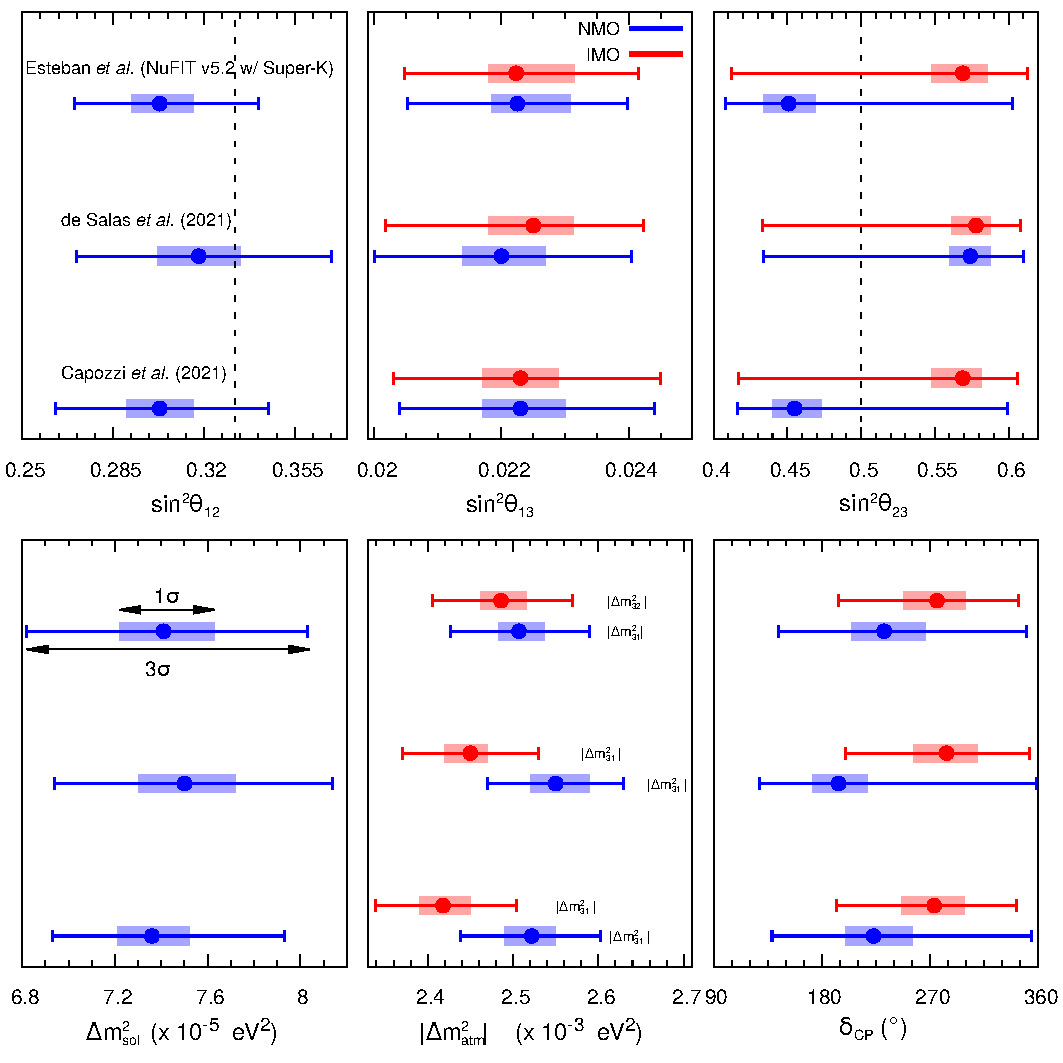
\includegraphics[width=\linewidth]{./Figures/Chapter-4/multi_fit_params_edited.pdf}
	\caption{\footnotesize{Current $1\sigma$ (see rectangular boxes)  and $3\sigma$ (see horizontal lines) allowed ranges of the neutrino oscillation parameters obtained from the global fit studies performed by Esteban $et~ al.$~\cite{NuFIT}, de Salas $et~ al.$~\cite{deSalas:2020pgw}, and Capozzi $et~ al.$~\cite{Capozzi:2021fjo}. The blue (red) lines and boxes represent the values for NMO (IMO). In each panel, the best-fit value of the respective oscillation parameter is shown by blue (red) dots for NMO (IMO).
Vertical black dashed lines in the panels related to $\sin^2\theta_{12}$ and $\sin^2\theta_{23}$ show their corresponding values in the tri-bimaximal mixing scheme. Note that the measurements of $\sin^{2}\theta_{12}$ and $\Delta m^{2}_{\mathrm{sol}}\, (\equiv \Delta m^{2}_{21})$ are not sensitive to the choice of mass ordering. }}
	\label{fig:1}
\end{figure}
%----------------------------------------

Fig.~\ref{fig:1} summarizes our current understanding of the six neutrino oscillation parameters in the standard three-neutrino framework. It confirms that we have already attained a remarkable precision on solar oscillation parameters ($\Delta m^2_{21}$ and $\sin^2\theta_{12}$), atmospheric mass-splitting ($\Delta m^2_{31}$), and reactor mixing angle ($\theta_{13}$). In this figure, we compare the $1\sigma$ (shown with colored rectangular blocks) and $3\sigma$ allowed (shown with horizontal lines) regions of the oscillation parameters that have been calculated by doing a combined analyses of the existing global oscillation data~\cite{NuFIT,deSalas:2020pgw, Capozzi:2021fjo, Esteban:2020cvm}. These works take into account the data from the Solar (Gallex and GNO~\cite{Cleveland_1998}, SAGE~\cite{SAGE:2009eeu}, the four phases of Super-K (SK I-IV)~\cite{Super-Kamiokande:2005wtt, Super-Kamiokande:2008ecj, Super-Kamiokande:2010tar}, SNO~\cite{SNO:2011hxd}, and Borexino I-III~\cite{Bellini:2011rx, Borexino:2008fkj, BOREXINO:2014pcl}), atmospheric (IceCube/DeepCore~\cite{IceCube:2014flw, IceCube} and the four phases of Super-K (SK I-IV)~\cite{Super-Kamiokande:2017yvm, data-superk}), reactor (KamLAND~\cite{KamLAND:2013rgu}, Daya Bay~\cite{DayaBay:2018yms}, and RENO~\cite{RENO:2018dro, reno}), and the accelerator experiments (MINOS~\cite{MINOS:2013utc, MINOS:2013xrl}, T2K~\cite{t2k}, and NO$\nu$A~\cite{nova}). All the three studies find that the earlier tension between Solar and KamLAND data has been reduced considerably after incorporating the recent results from Super-K Phase IV 2970 days of solar data (energy spectra and day-night asymmetry)~\cite{sk}. Additionally, both Esteban $et~ al.$~\cite{Esteban:2020cvm, NuFIT} and Capozzi $et ~al.$~\cite{Capozzi:2021fjo} also consider the recent Super-K Phase IV atmospheric data~\cite{sk}.

In Fig.~\ref{fig:1}, the blue (red) regions are obtained assuming NMO (IMO). Note that in the case of the solar oscillation parameters $i.e.$ $\sin^2\theta_{12}$ and $\Delta m^2_{21}$, the IMO and NMO regions are identical. Vertical black dashed lines in the panels related to $\sin^2\theta_{12}$ and $\sin^2\theta_{23}$ depict their corresponding values in the tri-bimaximal mixing scheme~\cite{Harrison:2002er,Harrison:2002kp,King:2014nza}. 
Note that while Esteban $et~ al.$ and de Salas $et~ al.$ quote the values of atmospheric mass-splitting in terms of $\Delta m^{2}_{31}$, Capozzi $et~ al.$ express it in terms of $\Delta m^{2} = m^{2}_{3}- (m^{2}_{1} + m_{2}^{2})/2$, where $\Delta m^{2}_{31}$ = $\Delta m^{2} + \Delta m^{2}_{21}/2$ for both NMO and IMO.


A novel aspect of Fig.~\ref{fig:1} is that all three global fits now rule out $\delta_{\rm CP} \in \left[ 0, \sim135^\circ \right]$ at $3\sigma$ confidence level and $\delta_{\rm CP} \in \left[ 0, \sim180^\circ \right]$ at $1\sigma$ confidence level, while predicting the best-fit value to lie somewhere in the range $\left[ 200^\circ,~230^\circ \right]$. The constraint in $\delta_{\rm CP}$ is  essentially due to the data from T2K and NO$\nu$A as discussed earlier. As far as the neutrino mass ordering is concerned, all three global fits show preference for NMO, ruling out IMO at close to $2.5\sigma$~\cite{Esteban:2020cvm,NuFIT,Capozzi:2021fjo,deSalas:2020pgw}. Therefore, for the sake of simplicity, in this work, we show our results assuming NMO both in data and fit. We observe that the results do not change much for IMO.

Another important feature that emerges from Fig.~\ref{fig:1} is that the current $3\sigma$ allowed range in $\sin^2\theta_{23}$ is $\sim 0.4~ \rm{to}~ 0.6$. This range is still relatively large as compared to the current uncertainties on $\theta_{12}$ and $\theta_{13}$ and it spans on either sides of $\sin^2\theta_{23}  = 0.5$. The value $\sin^2\theta_{23}  = 0.5$ (or equivalently $\sin^22\theta_{23}  = 1$) corresponds to the case of maximal mixing (henceforth, referred to as {\it maximality}) between the $\nu_{2}, \, \nu_{3}$ and $\nu_{\mu}, \, \nu_{\tau}$ eigenstates, which can in principle allows for a complete flavor transition between $\nu_{\mu}$ and $\nu_{\tau}$. However, the recent global fit studies suggest that $\sin^2\theta_{23}$ $\neq$ 0.5 (see Fig.~\ref{fig:1}) or $\sin^22\theta_{23}  \neq 1$. This leads to the so-called octant degeneracy of $\theta_{23}$ $i.e.$ a lack of knowledge regarding whether $\theta_{23}$ is less than $45^\circ$ (denoted as lower octant, LO) or greater than $45^\circ$ (labelled as higher octant, HO)~\cite{Fogli:1996pv, Barger:2001yr, Minakata:2002qi, Minakata:2004pg, Hiraide:2006vh}. But before the question of octant of $\theta_{23}$ arises, it is vital to establish the exclusion of maximality at a high significance, which is the main thrust of this work. In Ref.~\cite{Capozzi:2021fjo}, the authors find a preference at 1.6$\sigma$ for $\theta_{23}$ in the LO with respect to the secondary best-fit in HO. They obtain a best-fit value of $\sin^{2}\theta_{23}$ = 0.455 in the LO assuming NMO and disfavor maximal $\theta_{23}$ mixing at $\sim$1.8$\sigma$. However, there is a slight disagreement between the three global fit studies as far as the measurement of $\theta_{23}$ is concerned (see top right panel in Fig.~\ref{fig:1}). In Ref. \cite{deSalas:2020pgw}, de Salas $et~ al.$ find a best-fit in the HO around $\sin^2\theta_{23} \sim 0.57$ assuming NMO, while Capozzi $et~ al.$~\cite{Capozzi:2021fjo} and Esteban $et~ al.$~\cite{Esteban:2020cvm} obtain the best-fit around $\sin^{2}\theta_{23} \sim 0.45$ in the LO. This difference in the best-fit value of $\sin^2\theta_{23}$ is probably due to the recent Super-K Phase I-IV 364.8 kt$\cdot$yrs of atmospheric data~\cite{sk} that only Capozzi $et~ al.$ and Esteban $et~ al.$ consider in their latest analyses.\\
\par The issue of non-maximal $\theta_{23}$ and the resolution of its octant (if $\sin^{2}2\theta_{23} \neq 1$) have far-reaching consequences as far as the models explaining neutrino masses and mixings are concerned~\cite{Mohapatra:2006gs, Albright:2006cw, Albright:2010ap, King:2013eh, King:2014nza}. Some examples of such models are quark-lepton complementarity~\cite{Raidal:2004iw, Minakata:2004xt,Ferrandis:2004vp, Antusch:2005ca}, $A_{4}$ flavor symmetry~\cite{Ma:2002ge,Ma:2001dn, Babu:2002dz,Grimus:2005mu, Ma:2005mw}, and $\mu$-$\tau$ permutation symmetry~\cite{Fukuyama:1997ky, Mohapatra:1998ka,Lam:2001fb, Harrison:2002et, Kitabayashi:2002jd, Grimus:2003kq, Ghosal:2003mq,Koide:2003rx, Mohapatra:2005yu}. The $\mu$-$\tau$ permutation symmetry is of particular interest since the current oscillation data strongly indicates that this symmetry is not exact in Nature. A high-precision measurement of 2-3 mixing angle and the measurement of its octant are inevitable to disclose the pattern of deviations from the above-mentioned symmetries, which in turn will help us to explain tiny neutrino masses and one small and two large mixing angles in the lepton sector~\cite{Xing:2014zka, Xing:2015fdg}. It has also been shown that without an accurate measurement of $\theta_{23}$, a precise measurement of $\delta_{\rm CP}$ will not be possible~\cite{Minakata:2013eoa}.

There are several studies in the literature addressing the issues related to the 2-3 mixing angle in the context of various neutrino oscillation experiments. For example, see Refs.~\cite{Antusch:2004yx, Minakata:2004pg, GonzalezGarcia:2004cu, Choudhury:2004sv, Choubey:2005zy, Indumathi:2006gr, Kajita:2006bt, Hagiwara:2006nn, Samanta:2010xm, Agarwalla:2013hma, Minakata:2013eoa, Ge:2013zua, Ge:2013ffa, Chatterjee:2013qus, Choubey:2013xqa, Bass:2013vcg, Coloma:2014kca, Bora:2014zwa, Das:2014fja,Nath:2015kjg, Ghosh:2015ena, Agarwalla:2016xlg, Ballett:2016daj}. In this work, we analyze in detail the sensitivities of the next generation, high-precision long-baseline neutrino oscillation experiment DUNE (Deep Underground Neutrino Experiment)~\cite{DUNE:2015lol, DUNE:2020lwj, DUNE:2020ypp, DUNE:2020jqi, DUNE:2021cuw, DUNE:2021mtg} to establish the deviation from maximal $\theta_{23}$ and to resolve its octant at high confidence level in light of the current neutrino oscillation data. While estimating DUNE's capability for the discovery of non-maximal $\theta_{23}$, we shed light on some relevant issues such as: (i) the individual contributions from appearance and disappearance channels, (ii) the impact of systematic uncertainties and marginalization over oscillation parameters, and (iii) importance of spectral analysis and data from both neutrino and antineutrino runs. We also study how much improvement DUNE can offer in the precision measurements of $\sin^{2}\theta_{23}$ and $\Delta m^2_{31}$ as compared to their current precision. While estimating the achievable precision on these parameters in DUNE, we also quantify the contribution from individual appearance and disappearance channels and demonstrate the importance of having both neutrino and antineutrino data.

The layout of this chapter is as follows. In Sec.~\ref{probability}, we discuss the potential of DUNE's baseline and energy in establishing deviation from maximal $\theta_{23}$ at the level of probabilities. Next, in Sec.~\ref{events}, we describe the key features of DUNE which are relevant for our numerical simulation and discuss the impact of possible correlations and degeneracies among $\sin^{2}\theta_{23}$, $\Delta m^{2}_{31}$, and $\delta_{\mathrm{CP}}$ at the level of total event rates, bi-events, and event spectra. In Sec.~\ref{results}, we quantify the performance of DUNE to establish non-maximal $\theta_{23}$. We also address several issues which are relevant to achieve the above-mentioned goals. In Sec.~\ref{conclusion}, we summarize our findings and make concluding remarks.\\
%%%%%%%%%%%%%%%%%%%%%%%%%%%%%%%%%%%%%%%%%%%%%
\section{Discussion at the level of probabilities}
\label{probability}
%%%%%%%%%%%%%%%%%%%%%%%%%%%%%%%%%%%%%%%%%%%%%%

%----------------------------------------------
\begin{table}[htb!]
		\label{tableprecision}

		\centering
		\resizebox{\columnwidth}{!}{%
			\begin{tabular}{|c|c|c|c|c|c|}
				\hline \hline
				\multirow{2}{*}{\textbf{Parameter}} & \multirow{2}{*}{\textbf{Best-fit}} & \multirow{2}{*}{\textbf{1$\sigma$ range}} & \multirow{2}{*}{\textbf{2$\sigma$ range}} & \multirow{2}{*}{\textbf{3$\sigma$ range}} & \textbf{Relative 1$\sigma$}\\
				& & & & &\textbf{Precision (\%)}\\
				\hline \hline
				$\Delta m^2_{21}/10^{-5}$ $\mathrm{eV^{2}}$ & 7.36 & 7.21 - 7.52 & 7.06 - 7.71 & 6.93 - 7.93 & 2.3\\
				\hline
				$\sin^{2}\theta_{12}/10^{-1}$ & 3.03 & 2.90 - 3.16 & 2.77 - 3.30 & 2.63 - 3.45 & 4.5\\
				\hline
				$\sin^{2}\theta_{13}/10^{-2}$ & 2.23 & 2.17 - 2.30 & 2.11 - 2.37 & 2.04 - 2.44 &  3.0\\
				\hline
				$\sin^2\theta_{23}/10^{-1}$ & 4.55 & 4.40 - 4.73 & 4.27 - 5.81 & 4.16 - 5.99 & 6.7 \\
				\hline
				$\Delta m^2_{31}/10^{-3}$ $\mathrm{eV^2}$ & 2.522 & 2.490 - 2.545 & 2.462 - 2.575 & 2.436 - 2.605 & 1.1\\
				\hline
				$\delta_{\text{CP}}$/$^\circ$ & 223  & 200 - 256 & 169 - 313 & 139 - 355 & 16\\
				\hline \hline
			\end{tabular}
			}
			\caption{\footnotesize{The benchmark values of the oscilation parameters and their corresponding ranges that we consider in our study assuming NMO. In second column, we mention the best-fit values as given in Ref.~\cite{Capozzi:2021fjo}. The third, fourth, and fifth columns depict the current 1$\sigma$, 2$\sigma$, and 3$\sigma$ allowed ranges, respectively under NMO scheme. The sixth column depicts the present relative 1$\sigma$ precision on various oscillation parameters as given in Ref.~\cite{Capozzi:2021fjo}.}}
			\label{table:one}
	\end{table}
%----------------------------------------

In the three-neutrino framework, the flavor eigenstates $\vert \nu_{\alpha}\rangle~\left(\alpha = e, \mu, \tau \right)$ and the mass eigenstates $\vert \nu_{i} \rangle ~\left(i=1,2,3\right)$ are connected by the $3\times3$ unitary Pontecorvo-Maki-Nakagawa-Sakata (PMNS) matrix $U$:
%-------------------------------------
\begin{equation}
\vert \nu_{\alpha}\rangle  = \sum_{i} U^\ast_{\alpha i}\vert\nu_{i} \rangle ~~~ {\rm and} ~~~
\vert \bar{\nu}_{\alpha} \rangle = \sum_{i} U_{\alpha i}\vert \bar{\nu}_{i} \rangle\, .
\end{equation}
%----------------------------------------
Following the standard Particle Data Group convention~\cite{Zyla:2020zbs}, the vacuum PMNS matrix $U$ is parametrized in terms of the three mixing angles ($\theta_{23}$, $\theta_{13}$, $\theta_{12}$) and one Dirac-type CP phase ($\delta_{\mathrm{CP}}$). The probability that a neutrino, with flavor $\alpha$ and energy $E$, after traveling a distance $L$, can be detected as a neutrino with flavor $\beta$ is given by
%-----------------------------
\begin{equation}
P_{\alpha\beta} = \delta_{\alpha\beta} - 4 \sum_{j>i} \mathcal{R} \left( U^\ast_{\alpha j}U_{\beta j} U_{\alpha i} U^\ast_{\beta i}\right)\sin^2\frac{\Delta m^2_{ji} L}{4E} + 2 \sum_{j>i} \mathcal{I} \left( U^\ast_{\alpha j}U_{\beta j} U_{\alpha i} U^\ast_{\beta i}\right)\sin\frac{\Delta m^2_{ji} L}{2E}\, ,
\end{equation}
%----------------------------
where, $\Delta m^2_{ji} = m^2_{j} - m^2_{i}$.
Approximate analytical expressions for oscillation probabilities including matter effect have been derived in Ref.~\cite{Akhmedov:2004ny}, retaining terms only up to second order in the small parameters $\sin^2\theta_{13}$ and $\alpha \left(\equiv \Delta m^2_{21}/\Delta m^2_{31}\right)$. The analytical expression for muon neutrino survival probability ($P_{\mu \mu}$) under the constant matter density approximation is given in Eq. 33 of Ref.~\cite{Akhmedov:2004ny}. Considering the current best-fit values of oscillation parameters (see second column in Table~\ref{table:one}), we have $\sin^2\theta_{13}\approx 0.02$, $\alpha \approx 0.03$, $\alpha\sin\theta_{13}\approx 0.004$, and $\alpha^2\approx 0.0008$. Therefore, ignoring the sub-leading terms which are of the order $\alpha^2$ and approximating $\cos \theta_{13}$ equal to 1, Eq. 33 of Ref. \cite{Akhmedov:2004ny} simplifies to
%---------------------------
\begin{eqnarray}
\label{pmumushort} 
  P_{\mu\mu} &\approx & 1 - M \sin^22\theta_{23} - N \sin^2\theta_{23} - R \sin 2\theta_{23} + T \sin 4\theta_{23} \, ,
\end{eqnarray}
%
\newpage
where,
\begin{align}
	\label{eqM}
	M =\;& \sin^2\Delta 
	- \alpha \cos^2\theta_{12}\,\Delta\sin2\Delta \nonumber\\
	&+ \frac{2}{\hat A -1}\sin^2\theta_{13}
	\bigg(
	\sin\Delta\,\cos(\hat A\Delta)\,
	\frac{\sin[(\hat A - 1)\Delta]}{\hat A - 1}
	- \frac{\hat A}{2}\,\Delta\sin2\Delta
	\bigg)\,,
\end{align}

%
%and
\begin{equation}
\label{eqN}
N = 4\sin^2\theta_{13}\frac{\sin^2(\hat A - 1) \Delta}{(\hat A-1)^2}\, ,
\end{equation}
%
\begin{equation}
\label{eqR}
R = 2\alpha\sin\theta_{13}\sin2\theta_{12}\cos\delta_{\rm CP} \cos\Delta\frac{\sin\hat A \Delta}{\hat A}\frac{\sin(\hat A - 1)\Delta}{\hat A - 1}\, ,
\end{equation}

and
\begin{equation}
\label{eqT}
T = \frac{1}{\hat{A}-1}\alpha\sin\theta_{13}\sin2\theta_{12}\cos\delta_{\rm CP}\sin\Delta\bigg(\hat A \sin\Delta - \frac{\sin \hat A \Delta}{\hat A}\cos(\hat A - 1)\Delta \bigg)\, .
\end{equation}
%----------------------
In the above equations, $\Delta \equiv \Delta m^{2}_{31}L/4E$ and $\hat{A} \equiv A/\Delta m^{2}_{31}$. The Wolfenstein matter term, $A = 2\sqrt{2}G_{F}N_{e}E = 7.6\times10^{-5} \times \rho~(\mathrm{g/cm^{3}}) \times E$ (GeV), where $G_{F}$ is the Fermi coupling constant, $N_{e}$ is the ambient electron density, $E$ is the energy of neutrino, and $\rho$ is the constant matter density through which neutrino propagates. In Eq.~\ref{pmumushort}, all the terms containing $\theta_{23}$ (see Eqs.~\ref{eqM} to~\ref{eqT}) provide crucial information to establish non-maximal $\theta_{23}$ and contribute towards the precision measurement of $\theta_{23}$, which are the focus of this work. The first term in Eq.~\ref{eqM}, which is proportional to $\sin^{2} {\Delta}$, is the leading term in muon neutrino survival channel and contributes the most to address the above-mentioned physics issues. The term in Eq.~\ref{eqN}, which is the leading term in $\nu_{\mu} \rightarrow \nu_{e}$ appearance channel, is suppressed by the small quantity $\sin^{2}\theta_{13}$, and the terms in Eqs.~\ref{eqR} and~\ref{eqT} are proportional to the quantitity $\alpha \sin \theta_{13}$ which is around $\sim 0.004$. Therefore, these terms provide sub-leading contributions towards establishing deviation from maximal mixing and to precisely measure the value of $\theta_{23}$. Note that the terms in Eqs.~\ref{eqR} and~\ref{eqT} are proportional to $\cos \delta_{\mathrm{CP}}$. These terms may help to measure the value of $\delta_{\mathrm{CP}}$, but they are blind to CP asymmetry. On the other hand, the terms in Eq.~\ref{eqN} and~\ref{eqT}, which are proportional to $\sin^{2}\theta_{23}$ and $\sin 4\theta_{23}$, respectively provide information on the octant of $\theta_{23}$. 

The main sensitivity to settle the octant of $\theta_{23}$ stems from $\nu_{\mu} \rightarrow \nu_{e}$ appearance channel ($P_{\mu e}$), which when expressed up to first order in $\alpha\sin\theta_{13}$ is given by (ignoring the term $\propto$ $\alpha^{2}$ and $\cos\theta_{13}\approx 1$)
%------------------------------------
\begin{equation}
\label{eqpmue}
P_{\mu e} \approx N \sin^2\theta_{23} + O \sin2\theta_{23}\cos\left(\Delta + \delta_{\mathrm {CP}}\right)\, ,
\end{equation}
%
where, 
\begin{equation}
\label{eqO}
O = 2\alpha\sin\theta_{13}\sin2\theta_{12}\frac{\sin\hat A \Delta }{\hat A}\frac{\sin(\hat A -1)\Delta }{\hat A-1}\, .
\end{equation}
%---------------------------------------
%
Note that the first term in Eq.~\ref{eqpmue} is sensitive to octant of $\theta_{23}$, while the second term is sensitive to CP phase $\delta_{\mathrm {CP}}$. This leads to an octant\,-\,$\delta_{\mathrm {CP}}$ degeneracy in the measurements made via appearance channel. However, this degeneracy can be resolved with the help of balanced neutrino and antineutrino data in appearance mode as discussed for the first time in Ref.~\cite{Agarwalla:2013ju}. Since, both the terms in $P_{\mu e}$ contain information on $\theta_{23}$ (see Eq.~\ref{eqpmue}), they contribute towards establishing deviation from maximal $\theta_{23}$ (see discussion in Sec.~\ref{appdisapp} and Fig.~\ref{fig:7}) and to precisely measure the value of $\sin^{2}\theta_{23}$. 

%----------------------------------
	\begin{figure}[htb!]
	\centering
	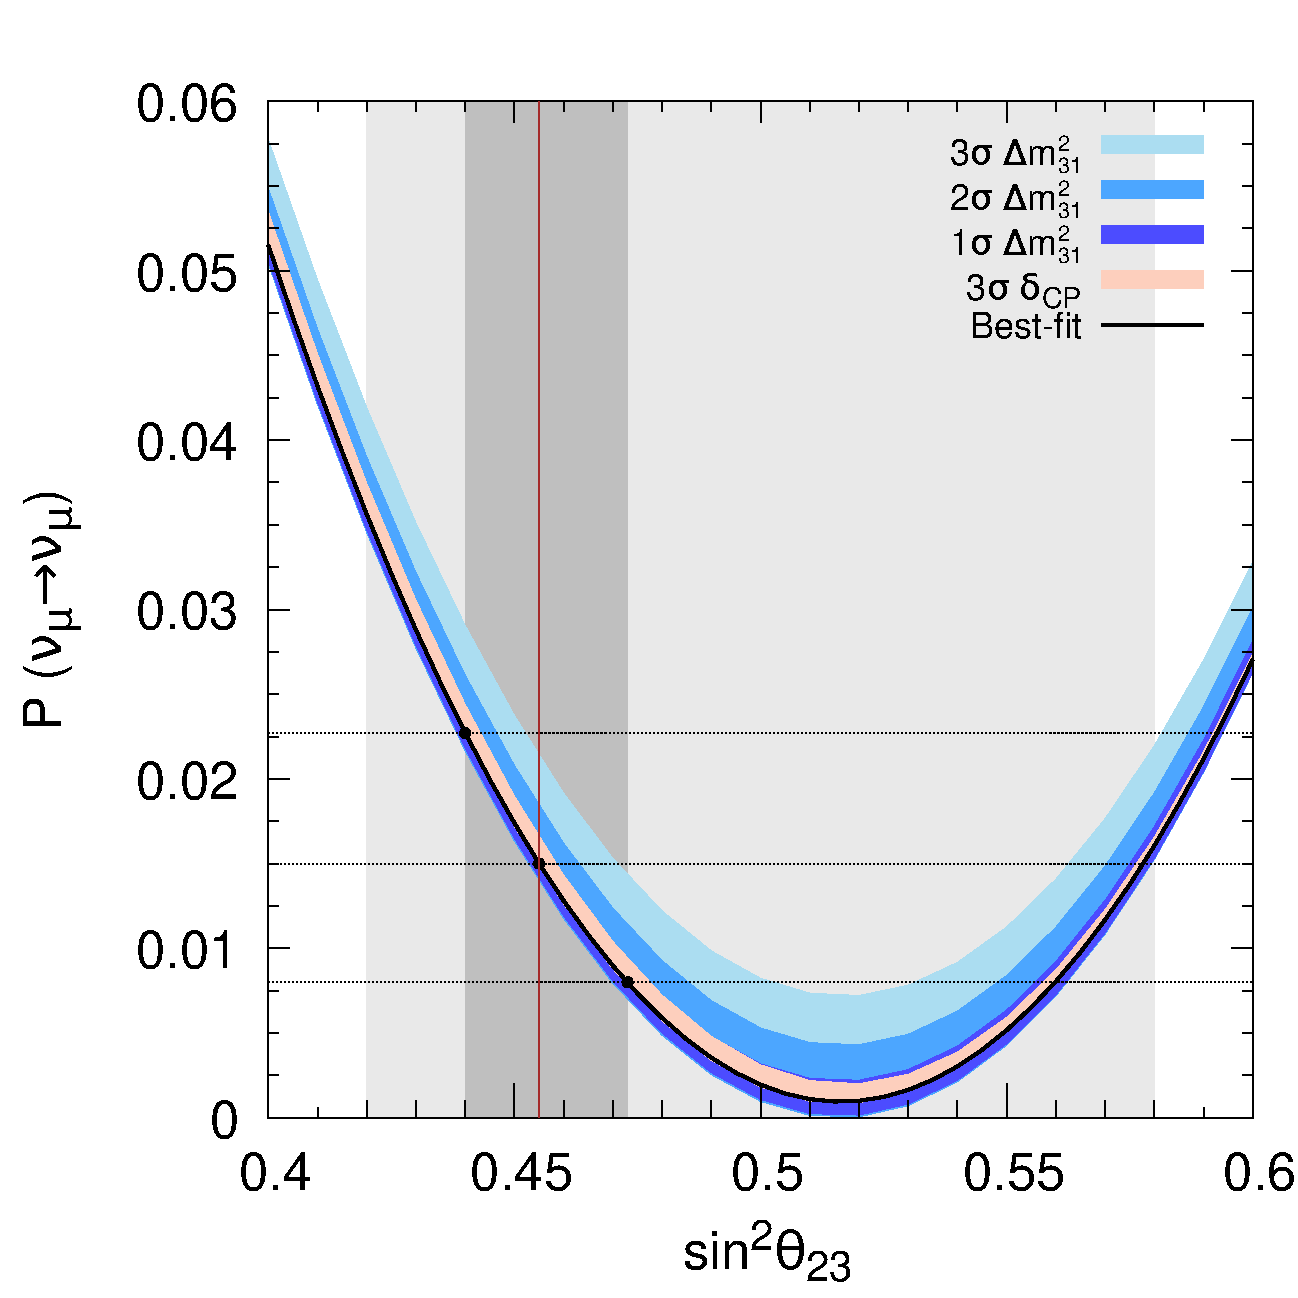
\includegraphics[width=0.49\linewidth]{./Figures/Chapter-4/Disappearance_nu_Bari_DUNE_NH.pdf}
	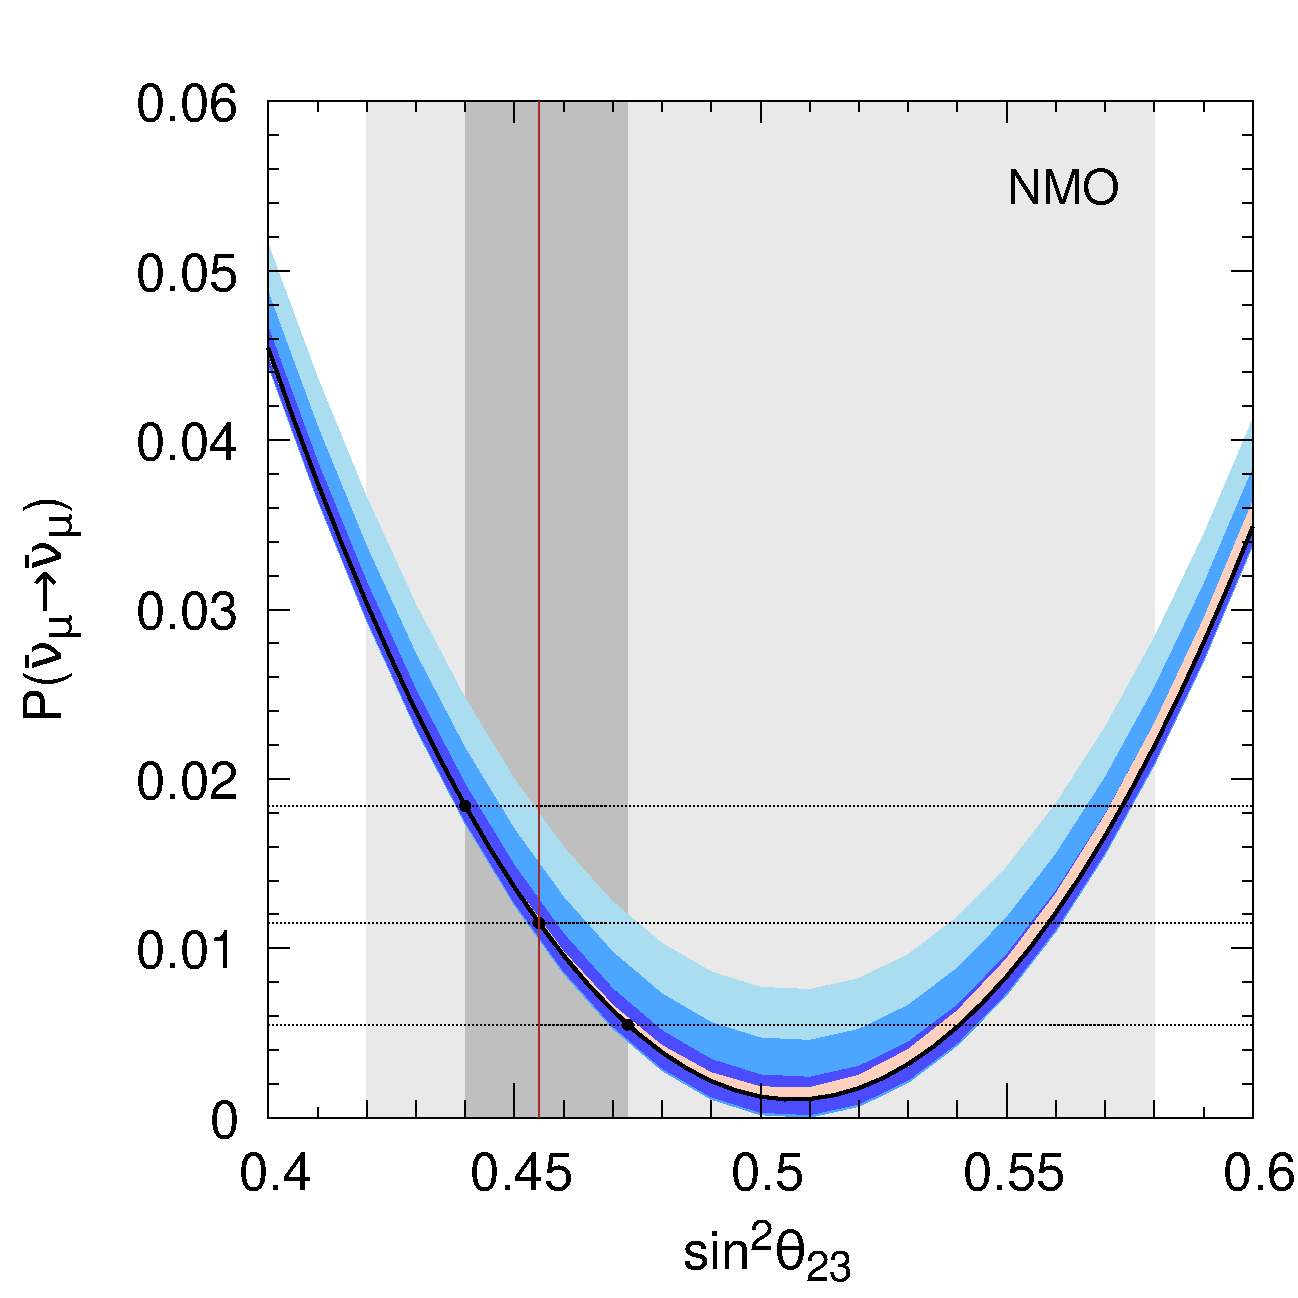
\includegraphics[width=0.49\linewidth]{./Figures/Chapter-4/Disappearance_anti_Bari_DUNE_NH.pdf}
	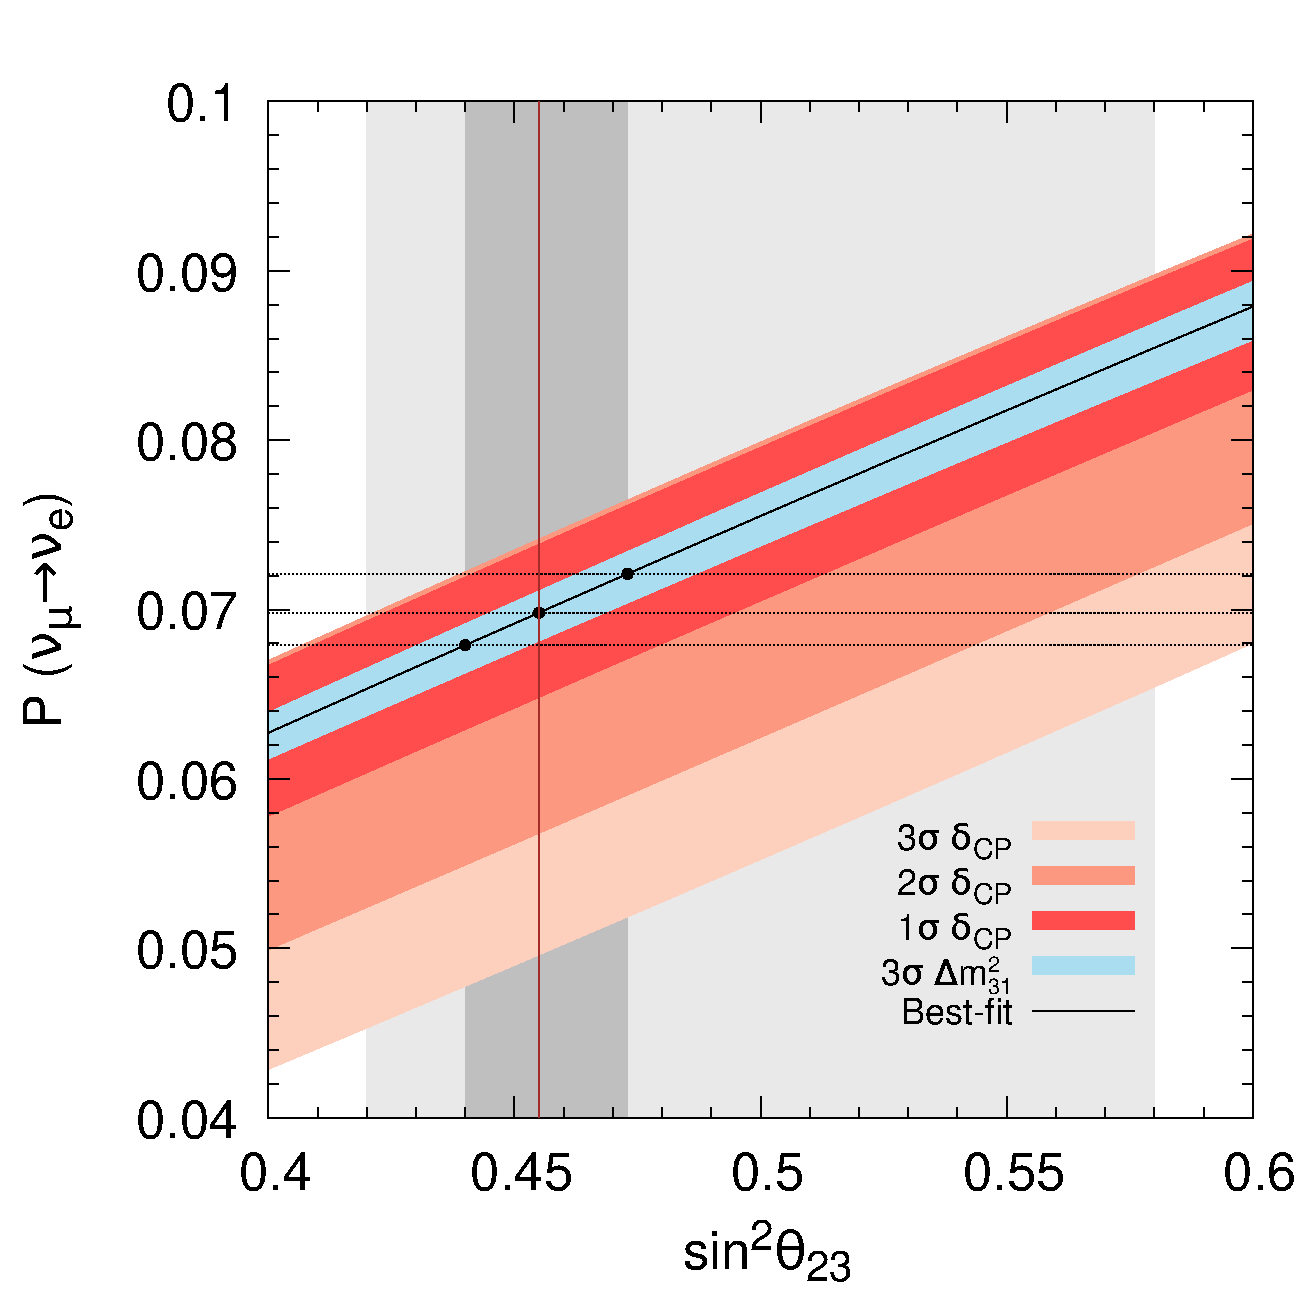
\includegraphics[width=0.49\linewidth]{./Figures/Chapter-4/Appearance_nu_Bari_DUNE_NH.pdf}
	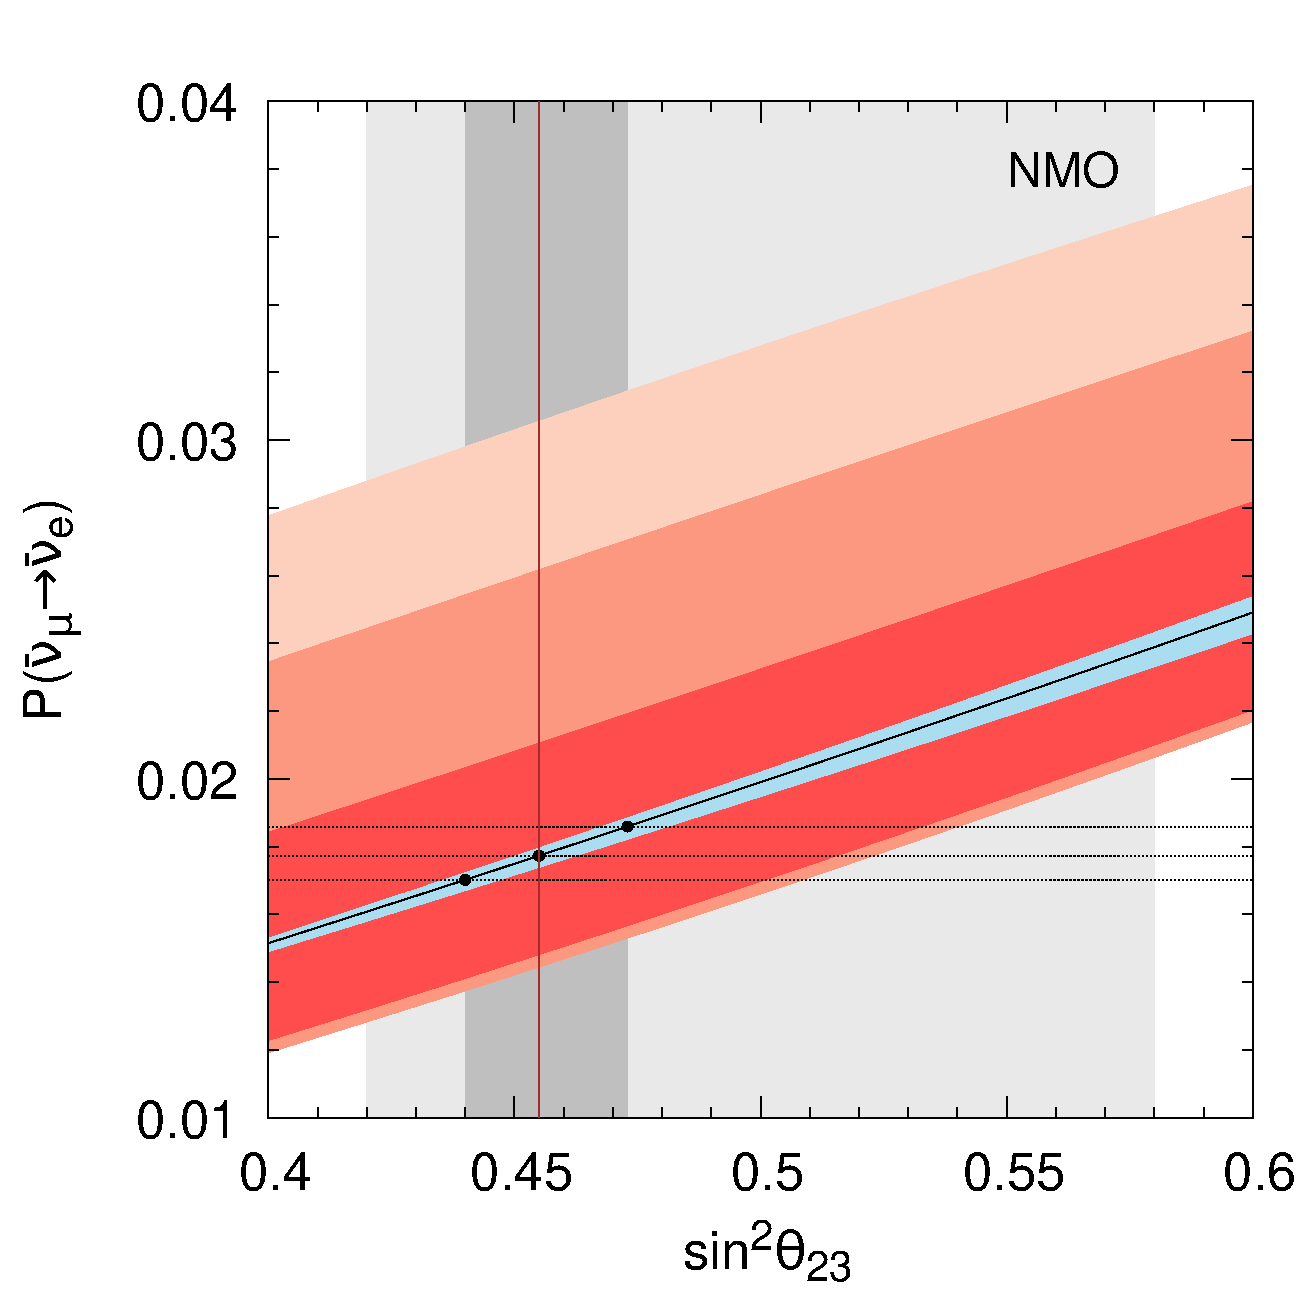
\includegraphics[width=0.49\linewidth]{./Figures/Chapter-4/Appearance_anti_Bari_DUNE_NH.pdf}
	\caption{\footnotesize{Probability as a function of $\sin^2\theta_{23}$ for $E = 2.5$ GeV, $ L=1284.9$ km, and $\rho=2.848~ \rm{g/cm}^{3}$ assuming NMO. The top (bottom) panels are for the disappearance (appearance) channel. The left (right) panels are for neutrino (antineutrino). The black solid curves show the probability considering the best-fit values of oscillation parameters as given in Table~\ref{table:one}. The three shaded blue (red) regions depict the variations in probability due to the present $1\sigma,~2\sigma,~\rm{and}~3\sigma$ allowed ranges in $\Delta m^2_{31}$ ($\delta_{\rm CP}$). The dark (light)-shaded grey area shows the currently allowed $1\sigma~ (2\sigma)$ region in $\sin^{2}\theta_{23}$ with the best-fit value of $\sin^{2}\theta_{23} = 0.455$ as shown by the vertical brown line. See Table~\ref{table:one} for details. Note that y-ranges are different in the bottom two panels.}}
	\label{fig:2}
\end{figure} 
%------------------------------------
To understand the role of oscillation channels $P_{\mu \mu}$ and $P_{\mu e}$ in distinguishing a non-maximal $\sin^{2}\theta_{23}$ from maximal mixing $i.e.$ $\sin^{2}\theta_{23} = 0.5$, we draw Fig.~\ref{fig:2}. In this figure, we show oscillation probabilities as a function of $\sin^2\theta_{23}$. To generate this figure, we use our benchmark values of the oscillation parameters and their corresponding ranges from Table~\ref{table:one}. The top panels are for $P_{\mu\mu}$ while the bottom panels are for $P_{\mu e}$. In the left (right) panels, we show the probabilities for neutrino (antineutrino).\\
The solid black curves in each of these figures show the probability corresponding to the best-fit values of $\Delta m^2_{31}$ and $\delta_{\rm CP}$ for each $\sin^2\theta_{23}$ whereas the different shades of blue and red bands correspond to the variation in probability due to $1,~2,$ and $3\sigma$ variations in $\Delta m^2_{31}$ and $\delta_{\rm CP}$, respectively. To generate these probabilities, we choose $ E = 2.5~\rm GeV$ and $ L=1284.9$ km which correspond to the DUNE's baseline and peak-energy fluxes. $E \sim 2.5~\rm GeV$ also corresponds to the first oscillation maximum (minimum) in $P_{\mu e}$ ($P_{\mu\mu}$). From Fig.~\ref{fig:2}, we make the following observations.\\
\begin{itemize}
\item 
$P_{\mu\mu}$ varies a lot as $\Delta m^2_{31}$ is varied while it changes only marginally with respect to $\delta_{\rm CP}$\footnote{$P_{\mu\mu}$ depends only on $\cos\delta_{\rm CP}$ at the sub-leading interference term proportional to $\alpha\sin^2\theta_{13}$. See Eq. 33 of Ref. \cite{Akhmedov:2004ny}.}.
%
The opposite behavior is seen in the case of $P_{\mu e}$ \cite{Coloma:2014kca, Minakata:2013eoa}. Therefore, we see significant degeneracies among the oscillation parameters $\Delta m^2_{31}$ and $\sin^2\theta_{23}$ in $P_{\mu\mu}$ channel. For $P_{\mu e}$ channel, the degeneracies are observed among $\delta_{\rm CP}$ and $\sin^2\theta_{23}$. 
%
\item 
For values of $\sin^2\theta_{23}$ in the HO which are very close to $\sin^2\theta_{23}=0.5$ $i.e.$ $\sin^2\theta_{23} \in [0.5, 0.53]$, $P_{\mu\mu}$ shows a flat behavior, which means that the slope of $P_{\mu\mu}$ is nearly 0. Also, note that the minimum of $P_{\mu\mu}$ occurs in HO, slightly away from $\sin^2\theta_{23} = 0.5$. It happens due to finite $\theta_{13}$ corrections~\cite{Raut:2012dm}. At the same time, for values of $\sin^2\theta_{23}$ in the LO which are very close to $\sin^2\theta_{23}=0.5$, $P_{\mu\mu}$ is steep. However, for values of $\sin^2\theta_{23}$ which are adequately far from $\sin^2\theta_{23}=0.5$, $P_{\mu\mu}$ is very steep in both LO and HO. We observe these features in both neutrino and antineutrino probabilities.

We can understand the above mentioned features in the following fashion. Let us consider only the first three terms on the R.H.S in Eq.~\ref{pmumushort}, neglecting the last two terms which are $\alpha \sin \theta_{13}$ suppressed. Now, it is easy to show that 

\begin{equation}
\frac{dP_{\mu\mu}}{d\sin^2\theta_{23}} \approx -\,4M\left(1-2\sin^2\theta_{23}\right) - N\, . 
\end{equation} 

Thus, $dP_{\mu\mu}/d\sin^2\theta_{23} \propto 1-2\sin^2\theta_{23}$ and therefore, $P_{\mu\mu}$ is steep when $\sin^2\theta_{23}$ is far from 0.5 and $P_{\mu\mu}$ is expected to be flat when $\sin^2\theta_{23}$ is close to 0.5. However, the minimum of $P_{\mu\mu}$ occurs when $dP_{\mu\mu}/d\sin^2\theta_{23} = 0 $, $i.e.$ at

\begin{equation}
\sin^2\theta_{23} \approx \frac{1}{2}\left(1+\frac{N}{4M}\right) \, . 
\end{equation}

Given that N and M are positive quantities, the minimum of $P_{\mu\mu}$ occurs in HO at a value larger than $\sin^2\theta_{23}$ = 0.5, but not at $\sin^2\theta_{23}$ = 0.5. This shift in the location of minimium of $P_{\mu\mu}$ is mainly governed by the N term, which is proportional to $\sin^{2}\theta_{13}$~\cite{Raut:2012dm}. Therefore, we observe a flat behavior in $P_{\mu\mu}$ around this shifted minimum in HO.

\item 
$P_{\mu e}$ shows a monotonic increase with respect to $\sin^2\theta_{23}$. This is true for both LO and HO, and in case of both neutrinos and antineutrinos. 
\end{itemize} 

Thus, based on the observations made above, we expect the results to have the following features: 
\begin{itemize}
%
\item Since, we expect the combination of $P_{\mu\mu}$ and $P_{\mu e}$ channels to resolve the degeneracies that are present in each of them individually, we do not expect the sensitivity to exclude non-maximal $\theta_{23}$, be too much affected by the choice of $\Delta m^2_{31}$ and $\delta_{\rm CP}$ within the given $3\sigma$ range. 
% 
\item For values of $\sin^2\theta_{23}$ in the HO and very close to 0.5, we expect that the sensitivity to establish deviation from maximality will come mainly from the appearance channel. However, for $\sin^2\theta_{23}$ values farther away from 0.5, the disappearance channel will contribute significantly. In the LO, we expect the main sensitivity to come from the disappearance channel even for $\sin^2\theta_{23}$ values very close to 0.5. 
%
\end{itemize} 
While the above arguments have been made using the probabilities calculated with a particular choice of $E = 2.5~\rm GeV$, we will see in the results section that these features hold in general.   

%%%%%%%%%%%%%%%%%%%%%%%%%%%%%%%%%%%%%%%%%%
\section{Discussion at the level of events}
\label{events} 
%%%%%%%%%%%%%%%%%%%%%%%%%%%%%%%%%%%%%%%%%%

We start this section by mentioning the salient features of DUNE which are crucial for our numerical simulations. Then, we show the total appearance and disappearance event rates in neutrino and antineutrino modes as a function of $\sin^{2}\theta_{23}$, $\Delta m^{2}_{31}$, and $\delta_{\mathrm{CP}}$ to establish some physics issues which are necessary to understand our main results. We also exhibit the bi-events plot in the plane of neutrino - antineutrino disappearance events and display their event spectra.

%---------------------------------------
\subsection{Salient features of DUNE}
\label{experiment}
%---------------------------------------

In order to calculate the expected event rates in DUNE and to estimate its sensitivity towards various physics issues, we use the publicaly available software GLoBES (General Long Baseline Experiment Simulator)~\cite{Huber:2004ka, Huber:2007ji}. We consider the simulation details as described in Ref.~\cite{DUNE:2021cuw}. DUNE will look for $\nu_{\mu}\rightarrow \nu_{\mu}$ (disappearance) and $\nu_{\mu}\rightarrow \nu_{e}$ (appearance) oscillations in both neutrino and antineutrino modes. Neutrinos are produced at the LBNF's Main Injector in Fermilab, Illinois, Chicago where protons of energy 120 GeV and power 1.2 MW are bombarded on a graphite target. This leads to the production of charged mesons which then decay in flight producing the neutrinos. Using the desired polarity in the horn-focusing system, neutrino or antineutrino mode can be selected. The neutrino flux at DUNE is wide-band with energies ranging from few hundreds of MeV to few tens of GeV, but the flux peaks at around $~$2.5 GeV with the majority of the flux lying in $1$ GeV to $5$ GeV region. 
%
These neutrinos first see a near detector (ND) placed 574 m downstream from the source and a far detector (FD) located roughly 5000 ft below the Earth's surface at the Sanford Underground Research Facility (SURF) in Lead, South Dakota, USA. The main purpose of ND is to precisely measure the unoscillated neutrino flux so as to reduce the systematic uncertainties related to fluxes. The distance between the source of production of neutrinos in Fermilab and the FD is 1284.9 km and the neutrinos traverse through Earth matter of roughly constant density of around $2.848~\rm g/cm ^{3}$. The FD is a 40 kt liquid argon time projection chamber (LArTPC) and is placed underground in order to minimize cosmogenic and atmospheric backgrounds. 
%
We consider a total run-time of 7 years equally divided in neutrino and antineutrino modes with a total of 1.1$ \times$ 10$^{21}$ protons on target (P.O.T.). This corresponds to a total exposure of 336 kt$\cdot$MW$\cdot$years equally shared in neutrino and antineutrino modes. 
The energy resolution of the FD in $\left(0.5 - 5\right)$ GeV range is around $\left(15 - 20\right)\%$. 
%
Our assumptions on systematic uncertainties are based on the material provided in Ref.~\cite{DUNE:2021cuw}. The errors are bin-to-bin correlated and are same for both neutrinos and antineutrinos. In the appearance channel $i.e.$ for the electron events, the normalization error is $2\%$ while for the disappearance channel $i.e.$ for the muon events, the normalization error is $5\%$. For the background events, the error varies from $5\%$ to $20\%$. 

%----------------------------------------
\subsection{Appearance and disappearance event rates as a function of $\sin^{2}\theta_{23},\ \Delta m^{2}_{31},$ and $\delta_{\rm CP}$}
%-----------------------------------------

In Table~\ref{table:two}, we show the total neutrino and antineutrino event rates for DUNE as a function of the oscillation parameters for both disappearance and appearance channels. The three columns correspond to LO ($\sin^2\theta_{23} = 0.455$) on the left, MM ($\sin^2\theta_{23} = 0.5$) in the center and HO ($\sin^2\theta_{23} = 0.599$) on the right. The central number in each cell, shown in boldface corresponds to the total number of events for the best-fit values of $\delta_{\rm CP} = 223^\circ$ and $\Delta m^2_{31} = 2.522\times 10^{-3}~\rm eV^2$, while considering $\sin^2\theta_{23}$ in LO, MM, and HO in second, third, and fourth columns, respectively. Rest of the oscillation parameters are kept at their respective best-fit values (see Table~\ref{table:one} for details). We determine other two numbers in the left and right (top and bottom) of central value by varying $\delta_{\rm CP}$ ($\Delta m^2_{31}$) from its central best-fit value to $3\sigma$ lower and upper bounds, respectively (as explained in the schematic diagram above Table~\ref{table:two}).

%----------------------------------------------
\begin{table}[htb!]
	\begin{center}
		\begin{small}
			\begin{tabular}{||c|c|c|c|c||}
			\hline \hline
			    \multicolumn{5}{||c||}{} \\
			    \multicolumn{5}{||c||}{$\mathcal{N}\left(223, 2.436\right)$} \\
			    \multicolumn{5}{||c||}{$\uparrow$} \\
			    \multicolumn{5}{||c||}{$\mathcal{N}\left(139, 2.522\right) \leftarrow \mathcal{N}\left(223, 2.522\right) \rightarrow \mathcal{N}\left(355, 2.522\right)$} \\
			    \multicolumn{5}{||c||}{$\downarrow$} \\
			    \multicolumn{5}{||c||}{$\mathcal{N}\left(223, 2.605\right)$} \\
			    \multicolumn{5}{||c||}{} \\
			    \multicolumn{5}{||c||}{$\mathcal{N}\left(x, y\right)$ where  $\mathcal{N}$: total number of events, $x$: $\delta_{\rm CP}$ in degrees, $y$: $\Delta m^2_{31}$ in $10^{-3}~\rm eV^2$ }\\
			    \multicolumn{5}{||c||}{} \\
			    \hline \hline
			    \multicolumn{5}{c}{} \\
%			    \multicolumn{5}{c}{} \\
			
				\hline\hline
				\multicolumn{2}{||c|}{Channel} & \text{LO}  & \text{MM} & \text{HO} \\
				\hline
				 &  & 1104  & 1193 & 1383 \\
				
				& & \boldsymbol{$\uparrow$} & \boldsymbol{$\uparrow$} & \boldsymbol{$\uparrow$}\\
				
			\multirow{5}{*}{\rotatebox[origin=c]{90}{Appearance}}& \text{$\nu$} &
				{820 $\leftarrow$$\boldsymbol{1121}$$\rightarrow$ 969}  & 				{908 $\leftarrow$$\boldsymbol{1211}$$\rightarrow$ 1058}  & 
								{1107 $\leftarrow$$\boldsymbol{1403}$$\rightarrow$ 1254}   \\
				
				& & \boldsymbol{$\downarrow$}& \boldsymbol{$\downarrow$}&\boldsymbol{$\downarrow$}\\
				
				& & 1135  & 1226 &
				1421 \\
				\cline{2-5}
				&  & 206  & 227 & 277 \\
				
				& & \boldsymbol{$\uparrow$}& \boldsymbol{$\uparrow$}&\boldsymbol{$\uparrow$}\\
				
				
				& \text{$\bar\nu$} & {267 $\leftarrow$$\boldsymbol{208}$$\rightarrow$ 258}  & {289 $\leftarrow$$\boldsymbol{230}$$\rightarrow$ 280}  & {338 $\leftarrow$$\boldsymbol{279}$$\rightarrow$ 329}   \\
				
				& & \boldsymbol{$\downarrow$}&\boldsymbol{$\downarrow$}&\boldsymbol{$\downarrow$}\\
				
				
				& & 210  & 232 & 281 \\
				\hline \hline
				 &  & 11018  & 10797 & 11249 \\
				
				& & \boldsymbol{$\uparrow$}& \boldsymbol{$\uparrow$}& \boldsymbol{$\uparrow$}\\
				
				\multirow{5}{*}{\rotatebox[origin=c]{90}{Disappearance}} & \text{$\nu$} & {10870 $\leftarrow$$\boldsymbol{10870}$$\rightarrow$ 10896}  & {10646 $\leftarrow$$\boldsymbol{10646}$$\rightarrow$ 10663}  & {11100 $\leftarrow$$\boldsymbol{11100}$$\rightarrow$ 11095} \\
				
				& & \boldsymbol{$\downarrow$}& \boldsymbol{$\downarrow$}&\boldsymbol{$\downarrow$}\\
				
				
				& & 10758  & 10532 & 10986 \\
				\cline{2-5}
				&  & 6397  & 6310 & 6565 \\
				
				& & \boldsymbol{$\uparrow$}&\boldsymbol{$\uparrow$}&\boldsymbol{$\uparrow$}\\
				
				
				&\text{$\bar\nu$} & {6306 $\leftarrow$$\boldsymbol{6306}$$\rightarrow$ 6280}  & {6219 $\leftarrow$$\boldsymbol{6219}$$\rightarrow$ 6193}  & {6477 $\leftarrow$$\boldsymbol{6477}$$\rightarrow$ 6452} \\
				
				& & \boldsymbol{$\downarrow$}&\boldsymbol{$\downarrow$}&\boldsymbol{$\downarrow$}\\
				
				
				
				& & 6234  & 6146 & 6406 \\
				\hline\hline
				
			\end{tabular}
		\end{small}
	\end{center}
	\caption{\footnotesize{Total appearance and diappearance event rates in $\nu$ and $\bar{\nu}$ mode. We assume 3.5 years of $\nu$ run and 3.5 years of $\bar{\nu}$ run and estimate the event rates for three different choices of $\sin^{2}\theta_{23}$: 0.455 (LO), 0.5 (MM), and 0.599 (HO). The central number in each cell corresponds to the current best-fit values of $\delta_{\rm CP}$ = 223$^{\circ}$ and $\Delta m^2_{31}$ = 2.522 $\times$ 10$^{-3}$ eV$^{2}$ assuming NMO. The other four numbers in each cell show the number of events corresponding to the present $3\sigma$ lower and upper bounds in $\Delta m^2_{31}$ (up and down arrows) and $\delta_{\rm CP}$ (left and right arrows). For clarity, see the schematic diagram given above this table.}}
	\label{table:two}
\end{table}
%----------------------------------------------

%----------------------------------------------------
\begin{figure}[htb!]
	\centering
	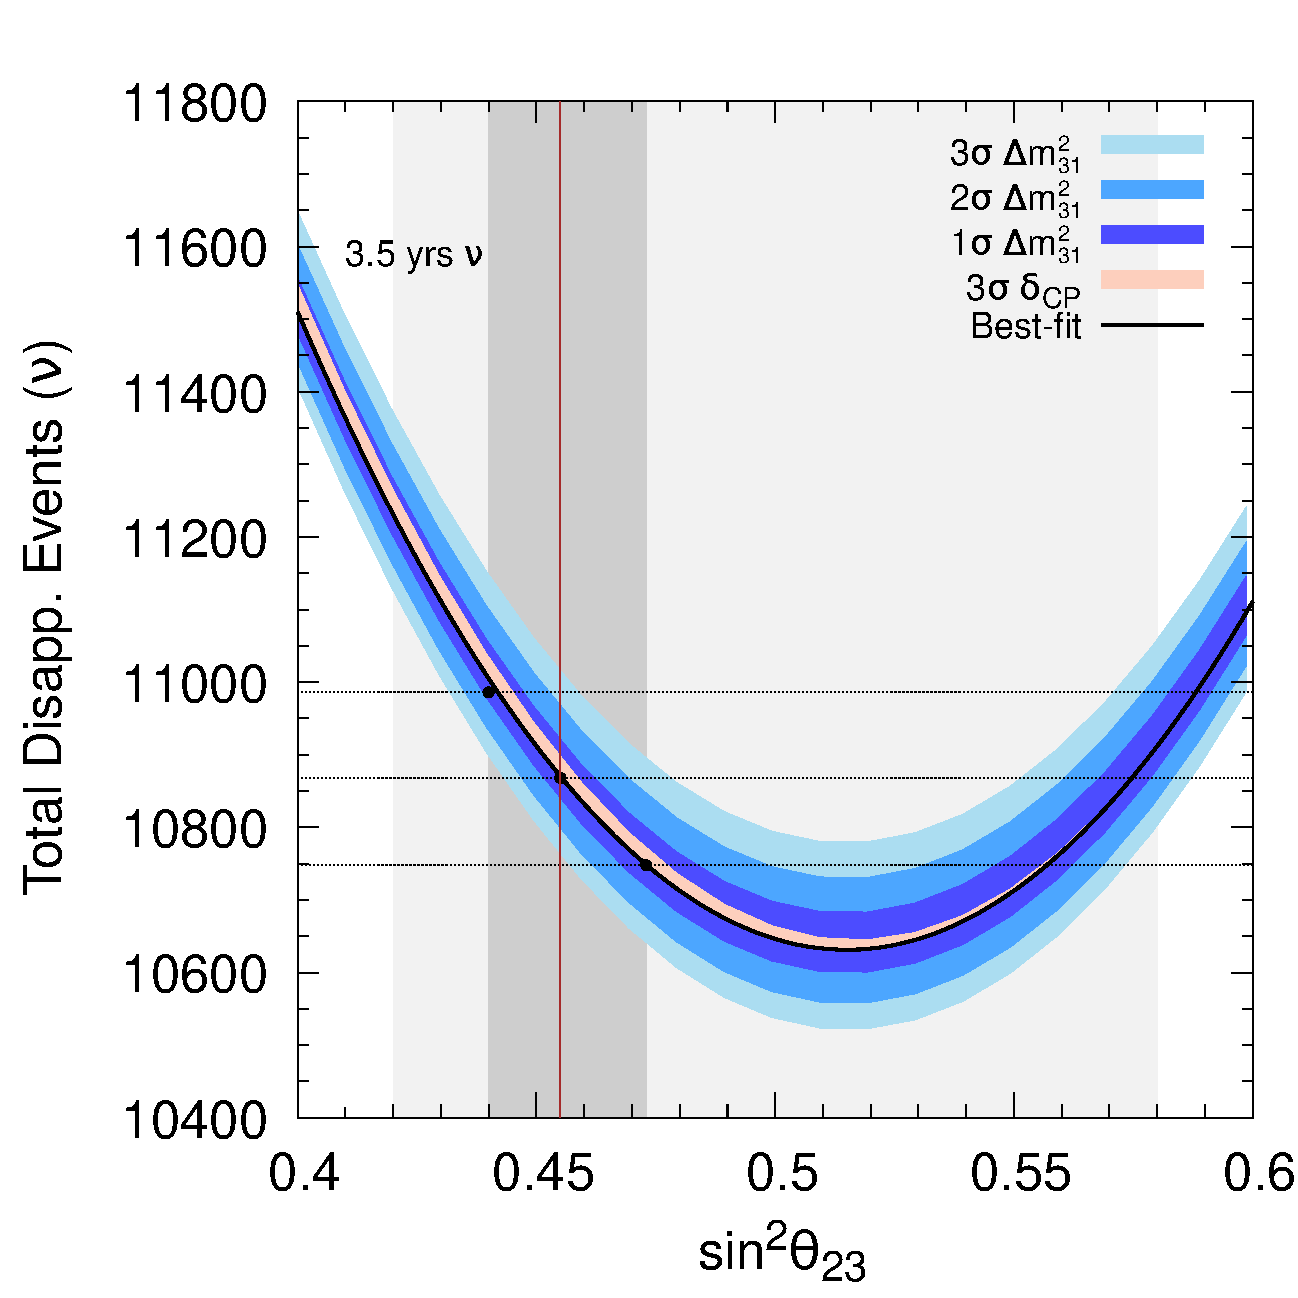
\includegraphics[width=0.49\linewidth]{./Figures/Chapter-4/Total_events_theta23_ldm_dcp_variation_NH_surv_nu}
	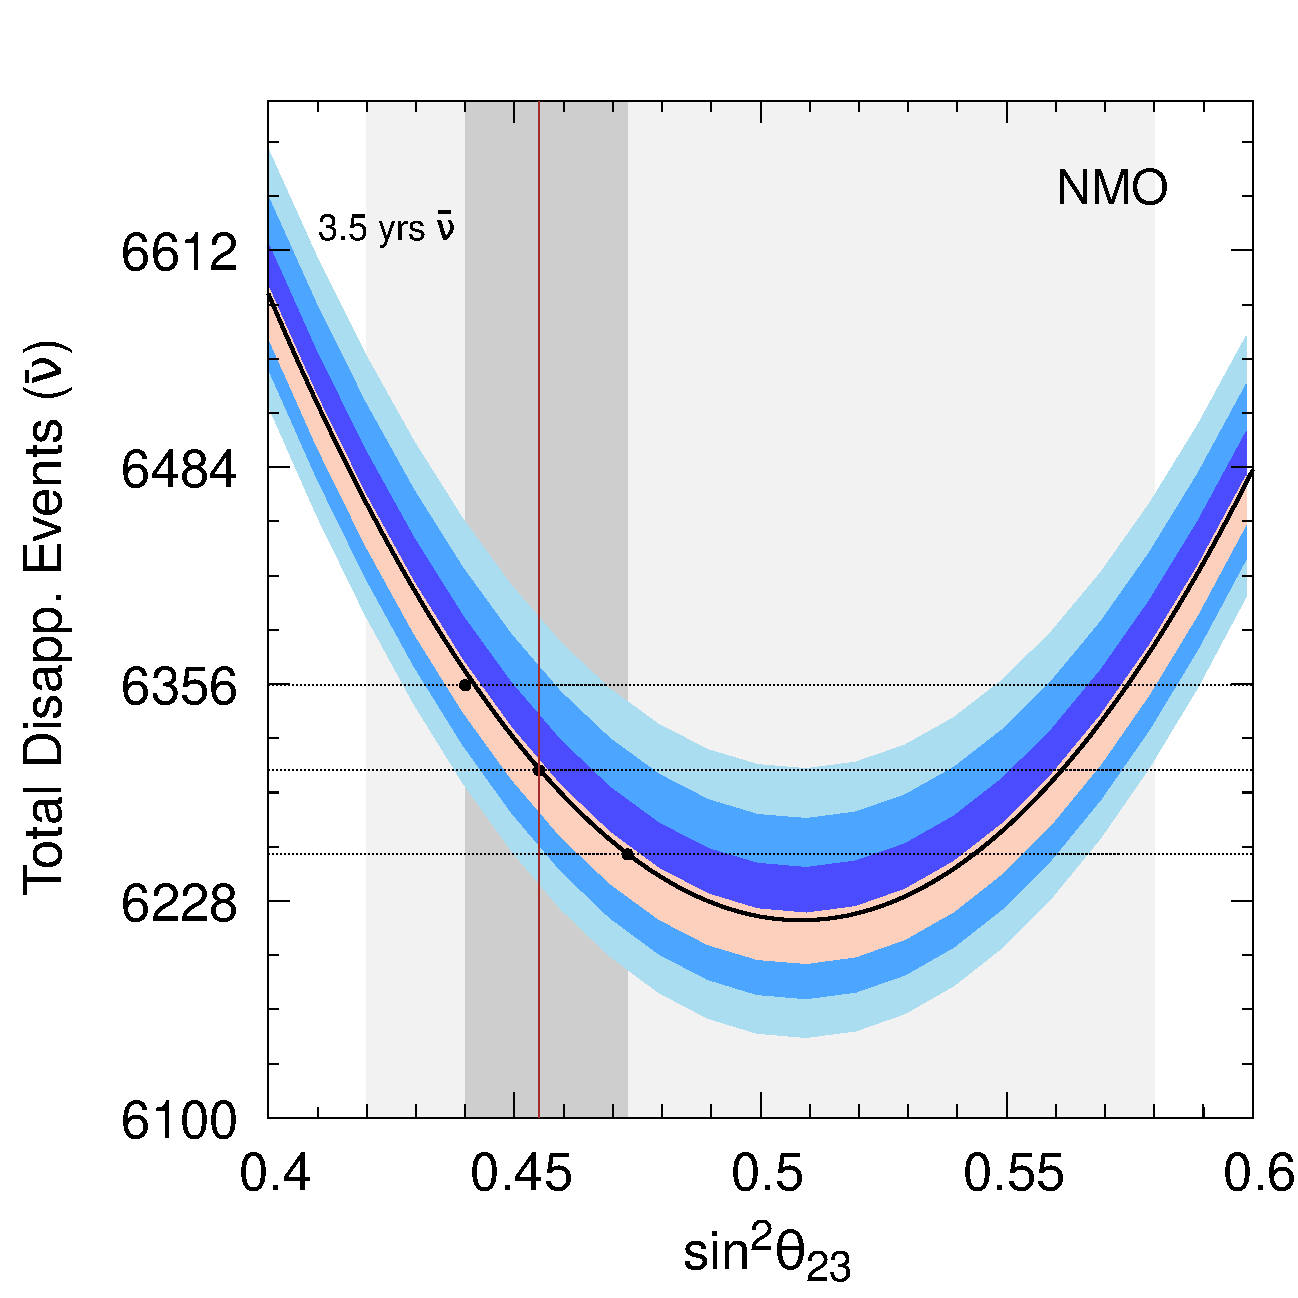
\includegraphics[width=0.49\linewidth]{./Figures/Chapter-4/Total_events_theta23_ldm_dcp_variation_NH_surv_anti}
	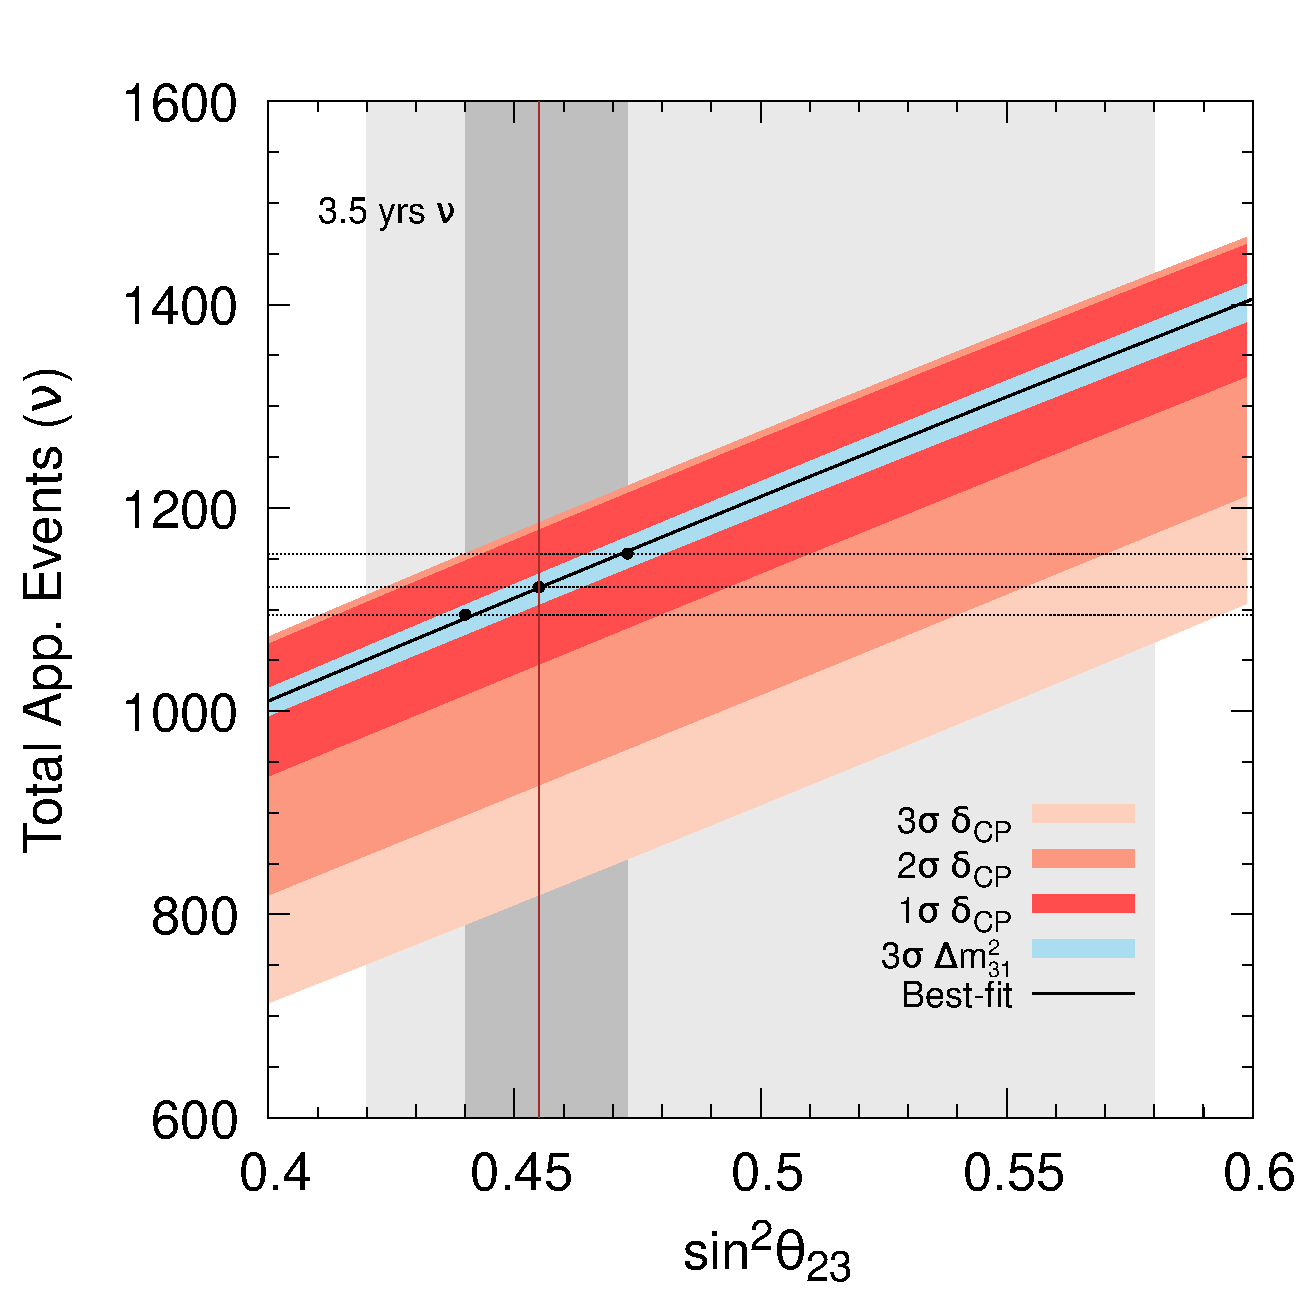
\includegraphics[width=0.49\linewidth]{./Figures/Chapter-4/Total_events_theta23_ldm_dcp_variation_NH_app_nu}
	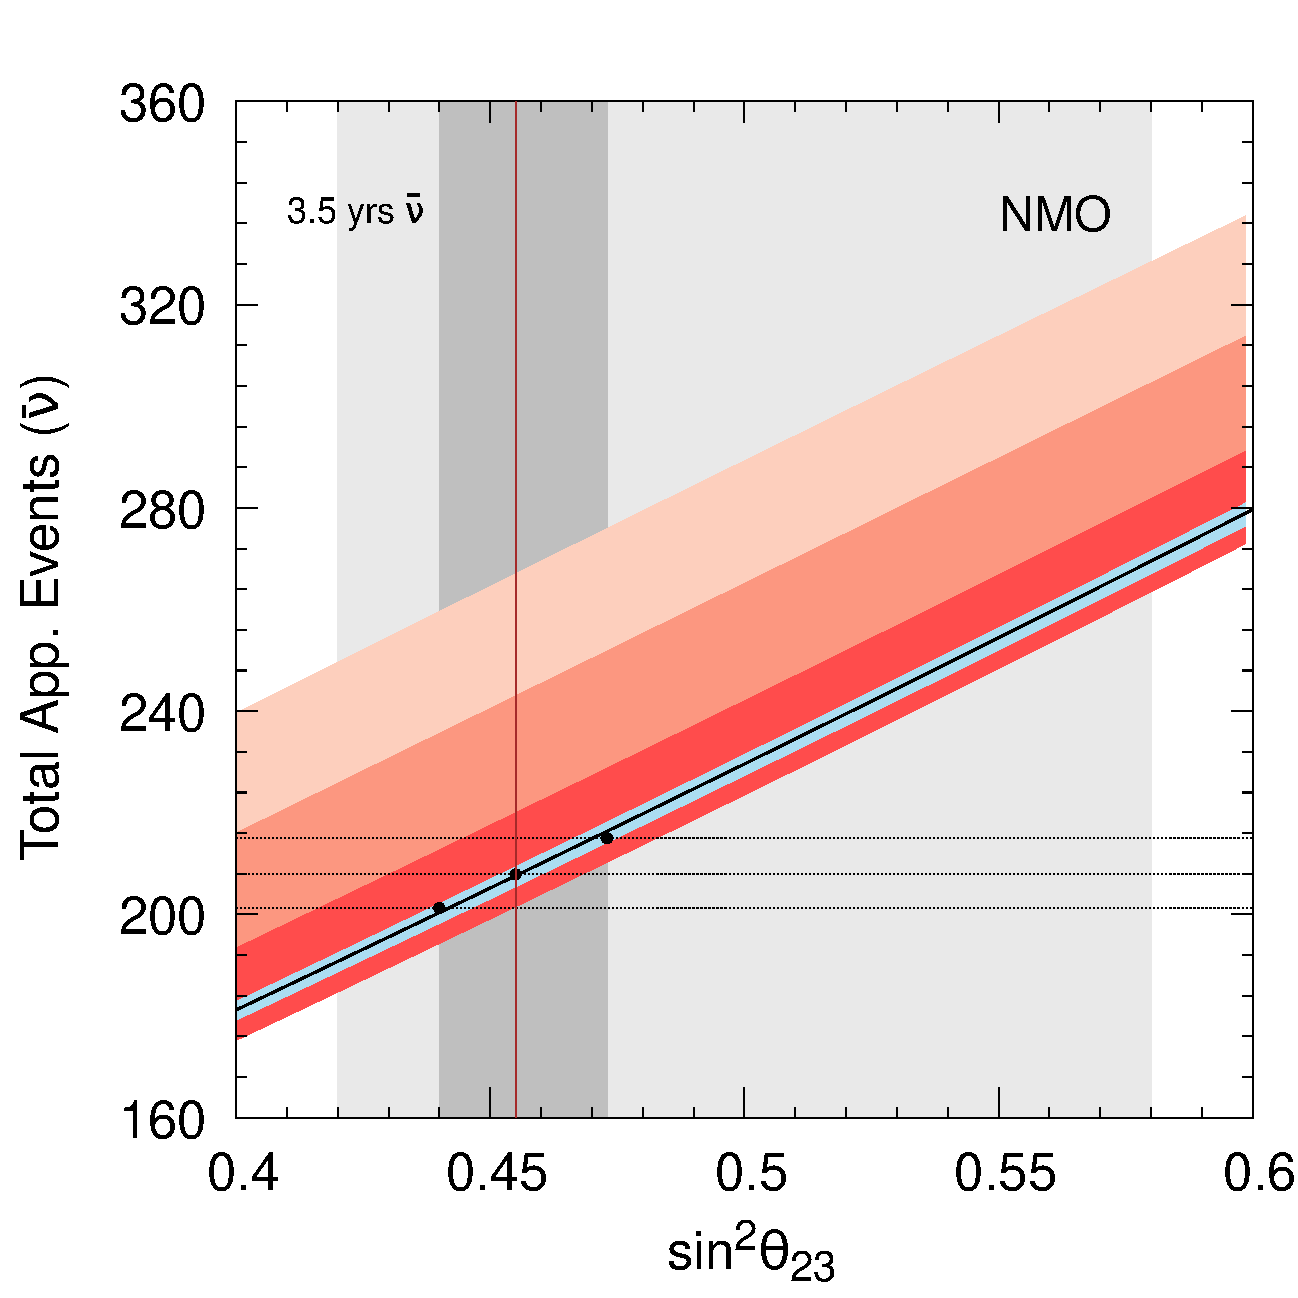
\includegraphics[width=0.49\linewidth]{./Figures/Chapter-4/Total_events_theta23_ldm_dcp_variation_NH_app_anti}
	\caption{\footnotesize{Total event rates as a function of $\sin^2\theta_{23}$ for DUNE assuming NMO. The top (bottom) panels are for disappearance (appearance) channel. The left (right) panels are for neutrino (antineutrino) assuming 3.5 years of run. The black solid curves show the event rates considering the best-fit values of oscillation parameters as given in Table~\ref{table:one}. The three shaded blue (red) regions show the variations in events due to present $1\sigma,~2\sigma,~ \rm{and}~3\sigma$ allowed ranges in $\Delta m^2_{31}$ ($\delta_{\rm CP}$). The dark (light)-shaded grey area shows the currently allowed $1\sigma~ (2\sigma)$ region in $\sin^{2}\theta_{23}$ with the best-fit value of $\sin^{2}\theta_{23} = 0.455$ as shown by the vertical brown line. See Table~\ref{table:one} and related text for details. Note that y-ranges are different in all the four panels. }}
	\label{fig:3}
\end{figure}
%----------------------------------------------------
From Table~\ref{table:two}, we note the following: 
\begin{itemize}
\item The appearance events change by a lot when $\sin^2\theta_{23}$ or $\delta_{\rm CP}$ is varied. This is observed in the case of both neutrino and antineutrino events. Thus, there are distinct $\theta_{23}$ - $\delta_{\rm CP}$ pairs which give same number of total events.  
\item The change in appearance events due to variation in $\Delta m^2_{31}$ is very small and the number of events in the three cases (best-fit, $3\sigma$ upper bounds, and 3$\sigma$ lower bounds) are almost degenerate. 
\item In the case of disappearance events, the central number for LO and HO are close to one another, but they are different from MM. The numbers also change significantly with respect to $\Delta m^2_{31}$. As far as $\delta_{\rm CP}$ variation is concerned, the event numbers show almost no change. Thus, in the case of disappearance events, there appears a $\sin^2\theta_{23}$ - $\Delta m^2_{31}$ degeneracy at the level of total rates.
\end{itemize} 
The observations made above are in line with the physics discussion done before in Sec.~\ref{probability} based on probabilities. As an example, we note that for 
$\nu$ appearance events, the numbers can vary between 820 to 969 for LO and 908 to 1058 for MM as $\delta_{\rm CP}$ is varied in the current $3\sigma$ range. Thus, there is a significant overlap in $\nu$ appearance events for LO and MM due to unknown $\delta_{\mathrm{CP}}$. However, for $\nu$ disappearance channel, the same oscillation parameter sets give number of events in the range 10870 to 10896 and 10646 to 10663, respectively, which may help to reduce the degenearcy as observed in appearance channel. The reverse argument can also be made where, for $\nu$ disappearance events, the numbers vary between 10758 to 11018 for LO and 10532 to 10797 for MM as $\Delta m^2_{31}$ is varied in its current $3\sigma$ range. But in the case of neutrino appearance channel, the corresponding events are lie in the range of 1104 to 1135 for LO and 1193 to 1226 for MM. Thus, the degeneracy that exists in the disappearance channel is partially resolved through the measurements made using appearance channel.

In Fig.~\ref{fig:3}, we show the disappearance (top panels) and appearance (bottom panels) event rates for various choices of $\sin^2\theta_{23}$ in the range $[0.4, 0.6]$. To generate this figure, we use the benchmark values of the oscillation parameters and their corresponding ranges as given in Table~\ref{table:one}. We see that the total event rates follow the same behavior as previously seen in Fig.~\ref{fig:2}, where we show $P_{\mu\mu}$ and $P_{\mu e}$ as a function of $\sin^2\theta_{23}$ assuming $E= 2.5~\rm GeV$. Note that though in Sec.~\ref{probability}, we discuss the main physics issues assuming a particular value of $E=2.5$ GeV, similar features are retained at the total event rates level as well in Fig.~\ref{fig:3}.


%----------------------------------------------------
\begin{figure}[htb!]
\centering
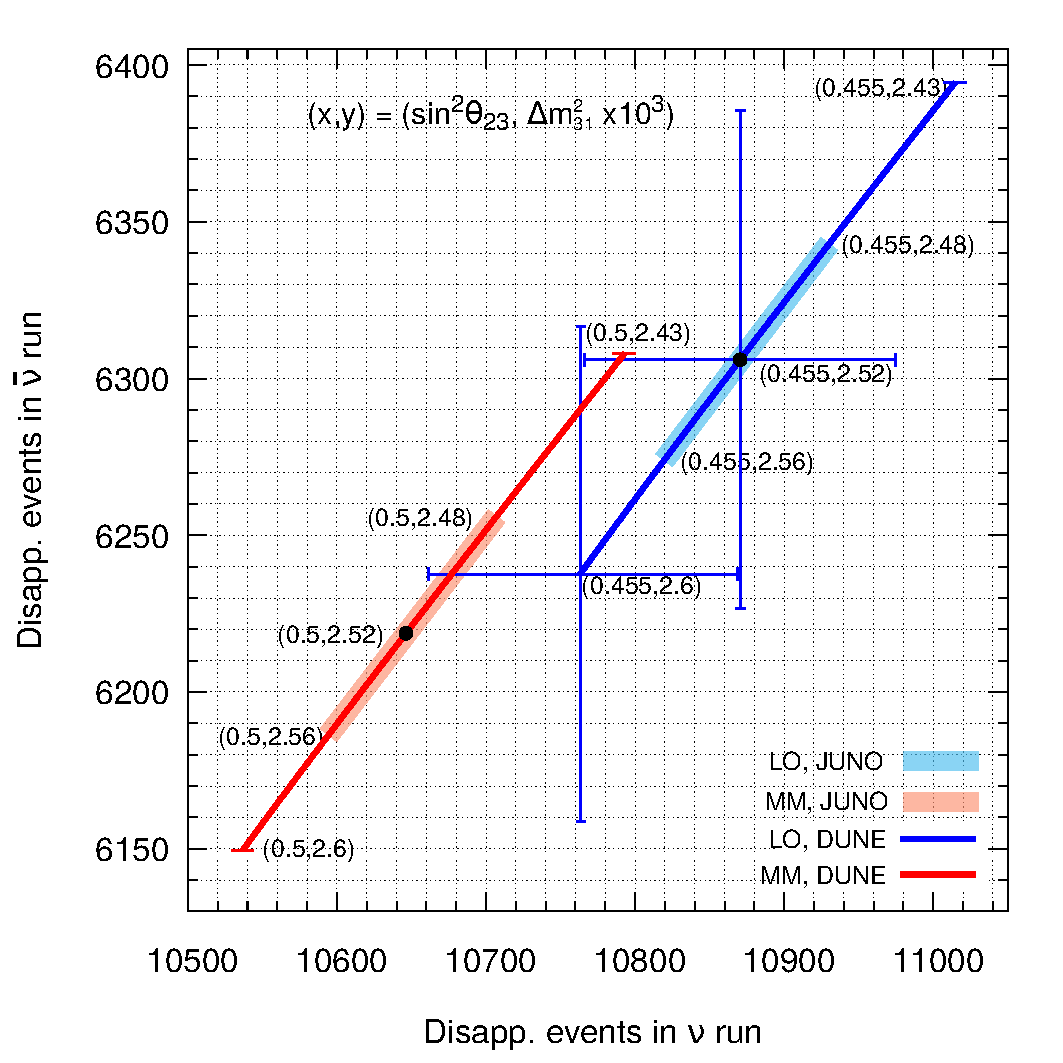
\includegraphics[width=0.63\linewidth]{./Figures/Chapter-4/bievent.pdf}
\caption{\footnotesize{Bi-events plot for DUNE in the plane of neutrino - antineutrino disappearance events assuming 336 kt$\cdot$MW$\cdot$years of exposure equally divided in neutrino and antineutrino modes. The blue line is obtained by varying $\Delta m^{2}_{31}$ in its 3$\sigma$ range of $[2.43 : 2.6] \times 10^{-3}~\rm{eV}^{2}$ with $\sin^2\theta_{23}=0.455$ (LO). The red line depicts the same with $\sin^2\theta_{23}=0.5$ (MM). The black dot on each line shows the disappearance events corresponding to the best-fit value of $\Delta m^2_{31} = 2.52 \times 10^{-3}$ eV$^{2}$. The values of other oscillation parameters are taken from Table~\ref{table:one} assuming NMO. The blue (red) rectangular region on blue (red) line portrays the variation in event rates due to 3$\sigma$ range in $\Delta m^{2}_{31}$ expected from JUNO~\cite{EPS-HEP-Conference2021, JUNO:2015zny}. The horizontal (vertical) error bars for the points [($\sin^{2}\theta_{23} = 0.455, \Delta m^{2}_{31} = 2.52 \times 10^{-3} \rm{eV}^{2}$) and ($\sin^{2}\theta_{23} = 0.455, \Delta m^{2}_{31} = 2.6 \times 10^{-3} \rm{eV}^{2}$)] show the 1$\sigma$ statistical uncertainties which are obtained by taking the square root of the $\nu \,(\bar{\nu})$ disappearance events.}} 
\label{fig:4}
\end{figure}
%----------------------------------------------------

In Fig.~\ref{fig:4}, we show the dependence of disappearance events on the oscillation parameters $\Delta m^2_{31}$ and $\sin^2\theta_{23}$ through the bi-events plot where we display the total neutrino (antineutrino) disappearance events on the x-axis (y-axis) assuming 3.5 years of run. We obtain blue curve by varying $\Delta m^{2}_{31}$ in its current 3$\sigma$ range of $[2.43 : 2.6] \times 10^{-3}~\rm{eV}^{2}$ assuming the current best-fit of $\sin^2\theta_{23}=0.455$ (see LO in legends). The red curve portrays the same with $\sin^2\theta_{23}=0.5$ (see MM in legends). The black dot on each line shows the disappearance events corresponding to the best-fit value of $\Delta m^2_{31} = 2.52 \times 10^{-3}$ eV$^{2}$. The values of other oscillation parameters are taken from Table~\ref{table:one} assuming NMO and $\delta_{\rm CP}$ = 223$^{\circ}$. The blue (red) rectangular region on blue (red) curve shows the variation in event rates due to allowed 3$\sigma$ range in $\Delta m^{2}_{31}$ as expected from JUNO~\cite{EPS-HEP-Conference2021, JUNO:2015zny}. The horizontal (vertical) error bars for the points [($\sin^{2}\theta_{23} = 0.455, \, \Delta m^{2}_{31} = 2.52 \times 10^{-3} \rm{eV}^{2}$) and ($\sin^{2}\theta_{23} = 0.455, \, \Delta m^{2}_{31} = 2.6 \times 10^{-3} \rm{eV}^{2}$)] show the 1$\sigma$ statistical uncertainties which are obtained by taking the square root of the neutrino (antineutrino) disappearance events.

The 1$\sigma$ statistical uncertainty in neutrino disappearance events corresponding to the benchmark oscillation parameters $\sin^2\theta_{23} = 0.455$ and $\Delta m^2_{31} = 2.522 \times 10^{-3}~\rm eV^2$ (see horizontal error bar around the black dot on blue line) has some overlap with the neutrino events on the red line. The same is true for antineutrino disappearance events (see the vertical error bar around the black dot on blue line). These overlapping regions due to 1$\sigma$ statistical fluctuations get reduced when we consider the variation in event rates for the allowed 3$\sigma$ range in $\Delta m^{2}_{31}$  (2.48 $\times$ 10$^{-3}$ eV$^2$ to 2.56$ \times$ 10$^{-3}$ eV$^2$, see rectangular red region) as expected from JUNO~\cite{EPS-HEP-Conference2021, JUNO:2015zny}. Therefore, we can conclude that based on only total event rates, a definitive exclusion of MM is not possible at high confidence level for the current best-fit values of oscillation parameters. We demonstrate later that the $\sin^2\theta_{23}$ - $\Delta m^2_{31}$ degeneracy that is present at the total event rates level can be resolved by including the spectral shape information along with total event rates and we can establish the deviation from maximal $\theta_{23}$ at high confidence level in DUNE. If we consider the event rates and their 1$\sigma$ statistical uncertainties corresponding to the oscillation parameters $\sin^2\theta_{23} = 0.455$ (current best-fit) and $\Delta m^2_{31} = 2.6 \times 10^{-3}~\rm eV^2$ (current 1$\sigma$ upper bound) on the blue line then we see more overlap with the event rates on the red line corresponding to MM solution. The overlap is less for the benchmark oscillation parameters $\sin^2\theta_{23} = 0.455$ (current best-fit) and $\Delta m^2_{31} = 2.43 \times 10^{-3}~\rm eV^2$ (current 1$\sigma$ lower bound) on the blue line.

%----------------------------------------------------
\subsection{Disappearance event spectra to resolve $\sin^{2} \theta_{23}-\Delta m^{2}_{31}$ degeneracy}
%----------------------------------------------------

%----------------------------------------------------
\begin{figure}[htb!]
	\centering
	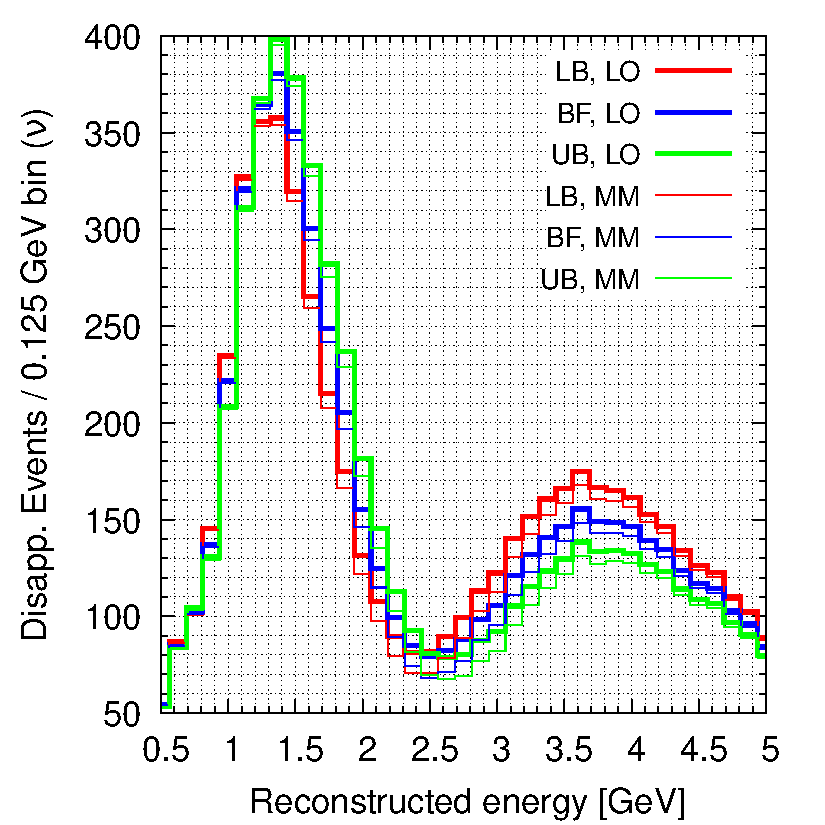
\includegraphics[width=0.49\linewidth]{./Figures/Chapter-4/New_MM_Events_NH_Hierarchies_surv_nu.pdf}
	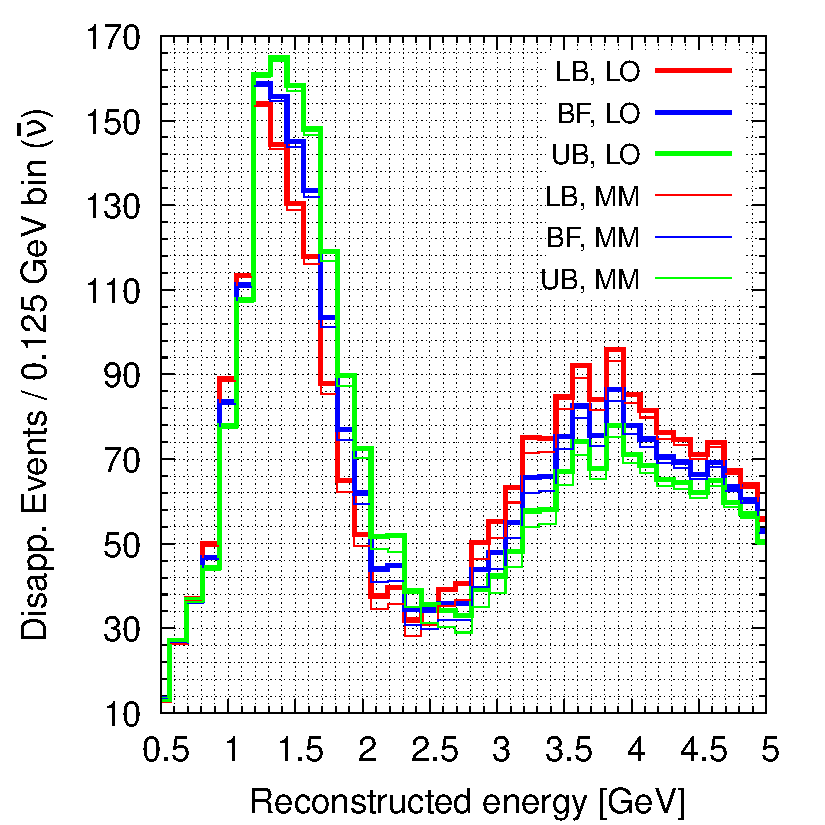
\includegraphics[width=0.49\linewidth]{./Figures/Chapter-4/New_MM_Events_NH_Hierarchies_surv_anti.pdf}
	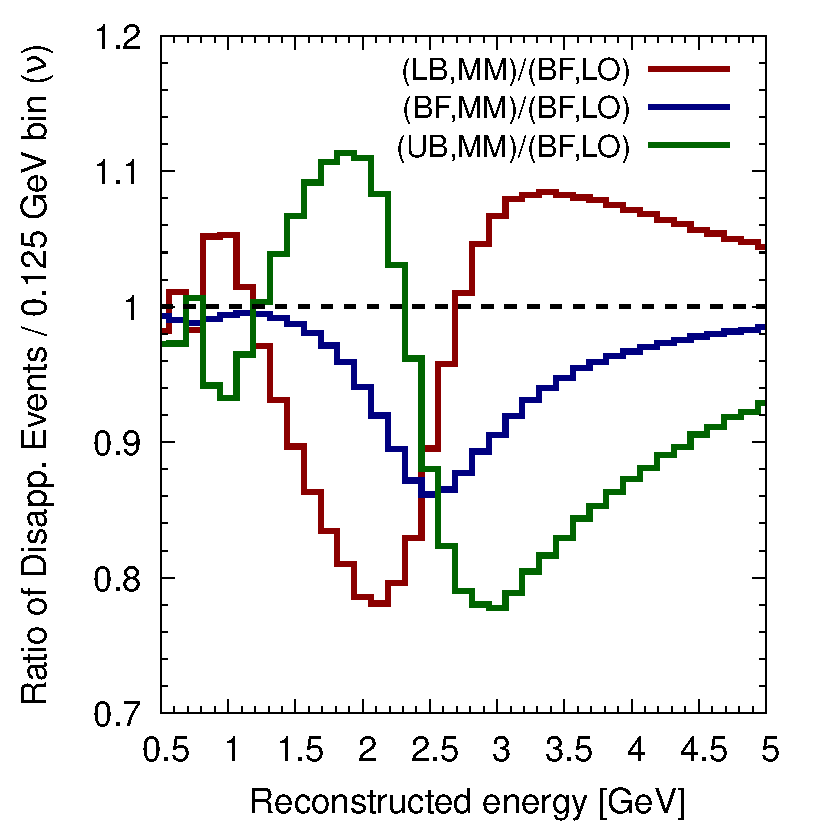
\includegraphics[width=0.49\linewidth]{./Figures/Chapter-4/Updated_Ratio_New_MM_Events_NH_Hierarchies_surv_nu.pdf}
	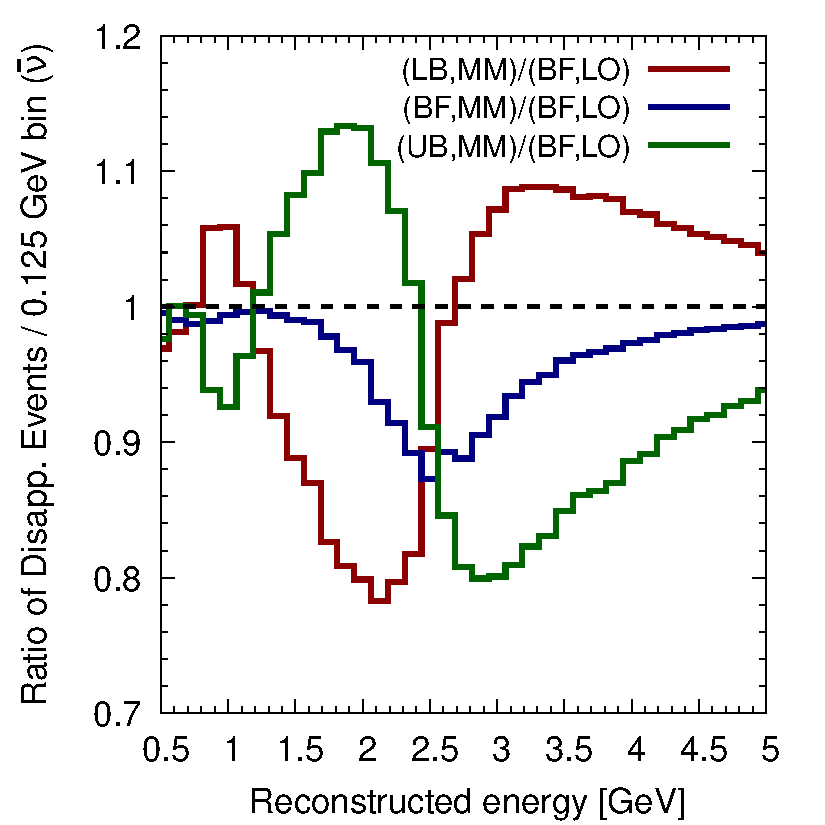
\includegraphics[width=0.49\linewidth]{./Figures/Chapter-4/Updated_Ratio_New_MM_Events_NH_Hierarchies_surv_anti.pdf}
	\caption{\footnotesize{In the top left (right) panel, we show the expected neutrino (antineutrino) disappearance event spectra as a function of reconstructed neutrino (antineutrino) energy assuming 3.5 years of $\nu$ ($\bar{\nu}$) run. The thick (thin) colored histograms correspond to a LO (MM) value of $\sin^{2}\theta_{23}$ = 0.455 (0.5). For a given value of $\sin^{2}\theta_{23}$, we depict the event spectra for three different choices of $\Delta m^2_{31}$: 2.522$\times 10^{-3}$ eV$^2$ [current best-fit (BF), blue lines], 2.436$\times 10^{-3}$ eV$^2$ [current 3$\sigma$ lower bound (LB), red lines], and 2.605$\times 10^{-3}$ eV$^2$ [current 3$\sigma$ upper bound (UB), green lines]. In the bottom left panel, we show the ratio of neutrino disappearance events in each energy bin as a function of reconstructed neutrino energy assuming 3.5 years of $\nu$ run. We present the same for antineutrino in the bottom right panel. The brown, blue, and green curves show the ratio of $N_{1}/{N}$, $N_{2}/{N}$, and $N_{3}/{N}$, respectively, where $N$: events in a given energy bin for $\left(\Delta m^2_{31} = 2.522\times 10^{-3}~\rm eV^2, \sin^2\theta_{23}=0.455\right)$, $N_{1}$: events in a given energy bin for $\left(\Delta m^2_{31} = 2.436\times 10^{-3}~\rm eV^2, \sin^2\theta_{23}=0.5\right)$, $N_{2}$: events in a given energy bin for $\left(\Delta m^2_{31} = 2.522\times 10^{-3}~\rm eV^2, \sin^2\theta_{23}=0.5\right)$, and $N_{3}$: events in a given energy bin for $\left(\Delta m^2_{31} = 2.605\times 10^{-3}~\rm eV^2, \sin^2\theta_{23}=0.5\right)$.
}}
	\label{fig:5}
\end{figure}
%--------------------------------------------------------

In Fig.~\ref{fig:5}, we show the event spectra for $\nu_{\mu}\rightarrow\nu_{\mu}$ disappearance channel as a function of the reconstructed neutrino energy. The top left (top right) panel is for neutrino (antineutrino) disappearance events. In the top panel, the thick and thin colored histograms correspond to a LO and MM value of $\sin^{2}\theta_{23}$, respectively. For a given value of $\sin^{2}\theta_{23}$, we exhibit the event spectra for three different choices of $\Delta m^2_{31}$: 2.522 $\times 10^{-3}$ eV$^2$ (BF, see blue lines), 2.436 $\times 10^{-3}$ eV$^2$ (LB, see red lines), and 2.605 $\times 10^{-3}$ eV$^2$ (UB, see green lines). Looking at Fig.~\ref{fig:5}, it seems that there is significant degeneracy between LO and MM when a full $3\sigma$ variation in $\Delta m^2_{31}$ is considered. However, on observing closely, it can be seen that the events for energy bins on either side of the oscillation minimum (maximum in the case of $P_{\mu e}$) at $ E = 2.5~GeV$ behave oppositely when $\Delta m^2_{31}$ is varied. This is made more evident in the lower panel of Fig.~\ref{fig:5} where the left (right) figure corresponds to neutrino (antineutrino). The three set of curves correspond to ratio of events in each reconstructed energy bin - $N_{i}/N$ (for $i =1,2,3$) where N is the number of events when $\sin^2\theta_{23} = 0.455$ and $\Delta m^2_{31} = 2.522 \, \times  10^{-3}~\rm eV^2$. In the ratio, $N_{1}, N_{2}, N_{3}$ are number of events when $\sin^2\theta_{23} = 0.5$ and $\Delta m^2_{31} = 2.438 \, \times 10^{-3}~\rm eV^2$, $2.522 \times 10^{-3}~\rm eV^2$, and $2.602 \times 10^{-3}~\rm eV^2$, respectively. It can be seen from the lower panels in Fig.~\ref{fig:5}, that the ratio of events approach 1 (reduction in sensitivity towards exclusion of maximality) on one side of the oscillation minimum while moving farther away from 1 compared to the blue line on the other side of the oscillation minimum. This explains that, while some of the energy bins decrease the sensitivity in deviation from the maximal choice of $\theta_{23}$, the other energy bins help to increase.  Therefore, we conclude that doing a spectral analysis further breaks the $\sin^2\theta_{23}$ - $\Delta m^2_{31}$ degeneracy seen in total event rates and therefore current 3$\sigma$ uncertainty in $\Delta m^2_{31}$ will not affect the sensitivity of DUNE in establishing non-maximal mixing of $\theta_{23}$. 


%%%%%%%%%%%%%%%%%%%%%%%%%%%%%%%%%%%%%%%%%%%%%%%%%
\section{Our findings}
\label{results}
%%%%%%%%%%%%%%%%%%%%%%%%%%%%%%%%%%%%%%%%%%%%%%%%%%

In this section, we demonstrate the capability of DUNE to address three important issues related to atmospheric oscillation parameter: (i) possible deviation of $\theta_{23}$ from maximal mixing (45$^{\circ}$), (ii) the correct octant of $\theta_{23}$ if it turns out to be non-maximal in Nature, and (iii) the achievable precision on the atmospheric oscillation parameters $\sin^2\theta_{23}$ and $\Delta m^2_{31}$ in light of current neutrino oscillation data. To estimate the median sensitivities in the frequentist approach~\cite{Blennow:2013oma}, we use the following definition of Poissonian $\chi^2$

\begin{equation}
\chi^2 (\vec{\omega}, \, \kappa_{s}, \, \kappa_{b})= \underset{( \vec{\lambda}, \, \kappa_{s}, \,\kappa_{b})}{\mathrm{min}}\left\{  2\sum_{i=1}^{n}(\tilde{y_i}-x_i-x_i\mathrm{ln}\frac{\tilde{y_i}}{x_i})+\kappa^2_{s}+ \kappa^2_{b}\right\}\, , 
\label{chi2} 
\end{equation}

where, n is the total number of reconstructed energy bins and 

\begin{equation}
\tilde{y_i}\,(\vec{\omega},\{\kappa_{s},\kappa_{b}\}) = N^{th}_i(\vec{\omega})[1+\pi^s\kappa_{s}]+N^b_i(\vec{\omega})[1+\pi^b\kappa_{b}]\, .
\label{chi}
\end{equation}
In the above equation, $N^{th}_i\,(\vec{\omega})$ denotes the predicted number of signal events in the $i$-th energy bin for a set of oscillation parameters $\vec{\omega} = \left\lbrace \theta_{23},\theta_{13},\theta_{12},\Delta \mathrm{m}^{2}_{21}, \Delta \mathrm{m}^{2}_{31},\delta_{\mathrm{CP}}\right\rbrace$ and $\vec{\lambda}$ is the set of oscillation parameters which we have marginalized in the fit. For an instance, when we address the issue of deviation from maximality, $\vec{\lambda} = \{\Delta m_{31}^2,~\delta_{\mathrm{CP}}\}$. $N^{b}_i\,(\vec{\omega})$ represents the number of background events in the $i$-th energy bin where the neutral (charged) current backgrounds are independent (dependent) on $\vec{\omega}$. The quantity $\pi^s$ ($\pi^b$) is the normalization uncertainty on signal (background). The quantities $\kappa_{s}$ and $\kappa_{b}$ are the systematic pulls~\cite{Huber:2002mx,Fogli:2002pt,Gonzalez-Garcia:2004pka} on signal and background, respectively. We incorporate the prospective data in Eq.~\ref{chi2} using the variable $x_{i}= N^{ex}_i\, +\, N^b_i$, where $N^{ex}_i$ denotes the observed charged current signal events in the $i$-th energy bin and $N^b_i$  represents the background as mentioned earlier.


%----------------------------------------------------
\subsection{Deviation from maximal $\theta_{23}$}
%----------------------------------------------------

As discussed previously in Fig.~\ref{fig:1}, the three global analyses of the oscillation data do not agree on the octant in which the best-fit value of $\theta_{23}$ lies. Further, they all find $\sin^2\theta_{23}=0.5$ to be allowed at $3\sigma$ confidence level.
Therefore, before we address the issue of resolving the octant of $\theta_{23}$, it is imperative to question at what confidence level maximal 2-3 mixing can be ruled out. We define $\Delta\chi^2$ for deviation from maximal $\theta_{23}$ as follows: 
\begin{equation}
\Delta \chi^2_{\rm DM}= \underset{(\vec{\lambda},~ \kappa_{s},\kappa_{b})}{\mathrm{min}}\left\{ \chi^2\left(\sin^2\theta_{23}^{\mathrm{true}} \in [0.4,0.6]\right) - \chi^2\left(\sin^2\theta_{23}^{\mathrm{test}} = 0.5\right)\right\},  
\end{equation} 
Here, $\vec{\lambda} = \{\delta_{\mathrm{CP}}, \, \Delta m^{2}_{31}\}$ are the oscillation parameters over which the $\Delta\chi^2$ has been marginalized, while $\kappa_{s}~\text{and}~ \kappa_{b}$ are the systematic pulls on signal and background, respectively.

%----------------------------------------------------
\begin{figure}[htb!]
	\centering
	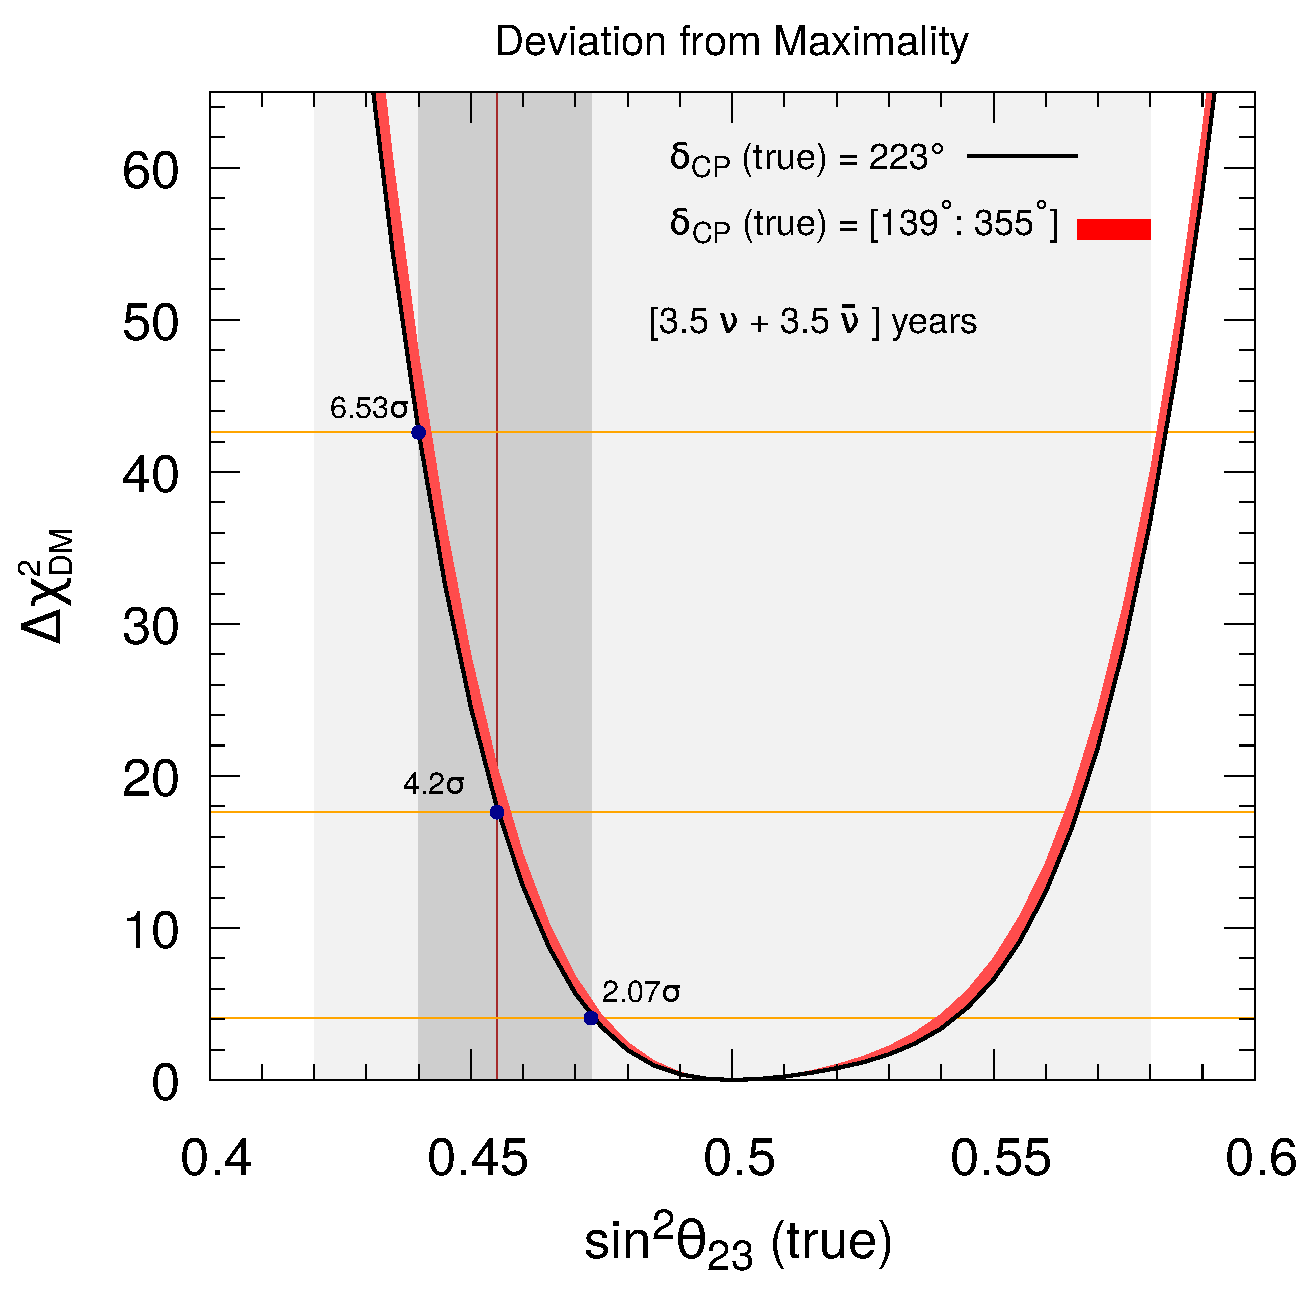
\includegraphics[width=0.49\linewidth]{./Figures/Chapter-4/All_channels_7yrs_octant_deviation_marg_223}
	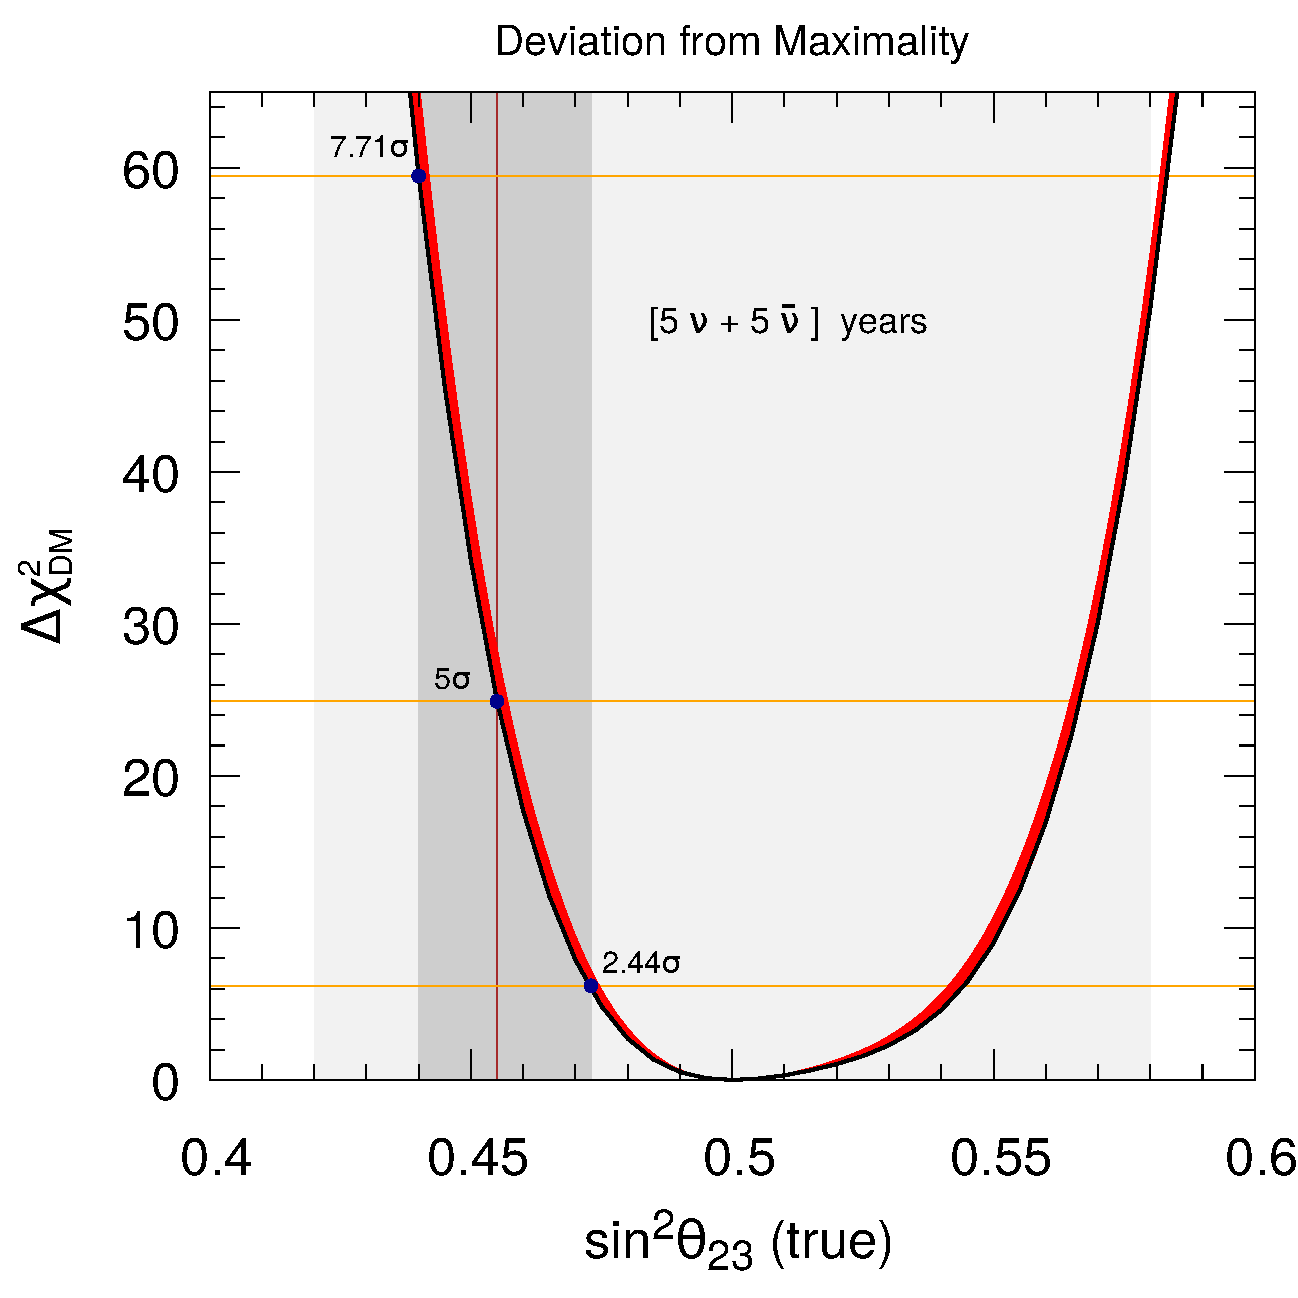
\includegraphics[width=0.49\linewidth]{./Figures/Chapter-4/All_channels_10yrs_octant_deviation_marg_223.pdf}
	\caption{\footnotesize{The black curve in the left (right) panel shows the potential of DUNE to establish the deviation from maximal $\theta_{23}$ as a function of true $\sin^2\theta_{23}$ assuming true NMO and $\delta_{\mathrm{CP}}$ (true) = 223$^{\circ}$ with 7 (10) years of total exposure equally divided in $\nu$ and $\bar{\nu}$ modes. The red bands portray the same for true $\delta_{\mathrm{CP}}$ in the range of 139$^{\circ}$ to 355$^{\circ}$. In the fit, we marginalize over the current 3$\sigma$ range of $\Delta m^{2}_{31} $ and $\delta_{\rm CP}$, while keeping rest of the oscillation parameters fixed at their present best-fit values as shown in Table~\ref{table:one}. The dark (light)-shaded grey area shows the currently allowed $1\sigma$ $(2\sigma)$ region in $\sin^{2}\theta_{23}$ as obtained in the global fit study~\cite{Capozzi:2021fjo} with the best-fit value of $\sin^{2}\theta_{23} = 0.455$ as shown by vertical brown line. The horizontal orange lines show the sensitivity (experessed in $\sigma = \sqrt{\Delta\chi^2_{\rm DM}}$) for the current best-fit and 1$\sigma$ upper and lower bounds of $\sin^2\theta_{23}$.}}
	\label{fig:6}
\end{figure}
%----------------------------------------------------

In Fig.~\ref{fig:6}, we show the potential of DUNE to establish deviation from maximal $\theta_{23}$ as a function of the true $\sin^2\theta_{23}$ in the range of 0.4 to 0.6. The black lines in both left and right panels display the ability of DUNE in establishing deviation from maximal $\theta_{23}$ assuming true NMO and $\delta_{\rm CP}$ (true) = 223$^{\circ}$. In the left panel, we show the results with nominal neutrino and antineutrino runs of 3.5 years each, while in the right panel we show results with 5 years of running in each mode. The red bands in Fig.~\ref{fig:6} portray the variation in $\Delta \chi^2_{\rm DM}$ for true $\delta_{\rm CP}$  in its current 3$\sigma$ allowed range of 139$^{\circ}$ to 355$^{\circ}$ (see Table~\ref{table:one}). Left panel reveals that for $\sin^2\theta_{23}$ (true) = 0.47 (current 1$\sigma$ upper bound), 0.455 (current best-fit), and 0.44 (current 1$\sigma$ lower bound), DUNE can exclude maximal mixing solution at 2.07$\sigma$, 4.2$\sigma$, and 6.5$\sigma$, respectively assuming true NMO and with a total 7 years of run (corresponds to a total exposure of 336 kt$\cdot$MW$\cdot$years) equally divided in neutrino and antineutrino modes. For a total 10 years of run (corresponds to a total exposure of 480 kt$\cdot$MW$\cdot$years), the above sensitivities get enhanced to 2.44$\sigma$, 5$\sigma$, and 7.71$\sigma$, respectively (see right panel). We observe that a 3$\sigma$ (5$\sigma$) determination of non-maximal $\theta_{23}$ is possible in DUNE with a total exposure of 7 years if the true value of $\sin^2\theta_{23} \lesssim 0.465~(0.450)$ or $\sin^2\theta_{23} \gtrsim 0.554~(0.572)$ for any value of true $\delta_{\mathrm{CP}}$ in its present 3$\sigma$ range and true NMO (see left panel). When we increase the total exposure from 7 years to 10 years, we see a marginal enhancement in the sensitivity (see right panel).

 %----------------------------------------------------
\subsubsection{Contributions from appearance and disappearance channels and role of systematics}
\label{appdisapp}
%----------------------------------------------------

%----------------------------------------------------
\begin{figure}[htb!]
	\centering
	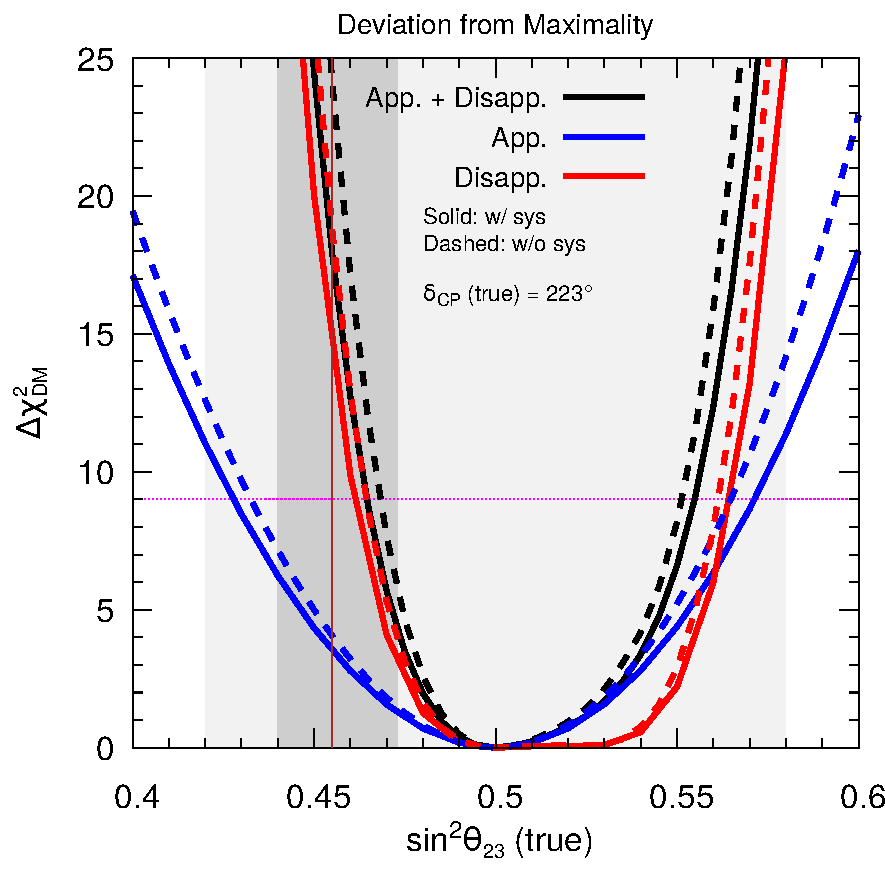
\includegraphics[width=0.65\linewidth]{./Figures/Chapter-4/Systematics_variation_All_channels_octant_deviation_marg_223.pdf}
	\caption{\footnotesize{Performance of DUNE to establish deviation from maximality as a function of true $\sin^2\theta_{23}$ assuming true NMO and $\delta_{\rm CP}$ (true) = 223$^\circ$ with 7 years of exposure equally divided in $\nu$ and $\bar{\nu}$ modes. Red, blue, and black curves show the sensitivity obtained using disappearance channel, appearance channel and their combinations, respectively. The solid (dashed) lines depict the results with (without) systematic uncertainties. In the fit, we marginalize over the current 3$\sigma$ range of $\Delta m^{2}_{31} $ and $\delta_{\rm CP}$, while keeping rest of the oscillation parameters fixed at their present best-fit values as shown in Table~\ref{table:one}. The dark (light)-shaded grey area shows the currently allowed $1\sigma$ $(2\sigma)$ region in $\sin^{2}\theta_{23}$ as obtained in the global fit study~\cite{Capozzi:2021fjo} assuming NMO with the best-fit value of $\sin^{2}\theta_{23} = 0.455$ as shown by vertical brown line. The capability of DUNE to establish non-maximal $\theta_{23}$ at 3$\sigma$ ($\Delta \chi^{2}_{\mathrm{DM}} = 9$) confidence level is shown by horizontal pink dotted line.}}
	\label{fig:7}
\end{figure}
%----------------------------------------------------

We now explore how the appearance and disappearance channels individually contribute towards the exclusion of MM. In Fig.~\ref{fig:7}, we show the $\Delta \chi^2_{\rm DM}$ as a function of true $\sin^2\theta_{23}$ for appearance (in solid blue), disappearance (in solid red) and combined (in solid black). It is interesting to note that for true  values of $\sin^2\theta_{23}$ in HO that are very close to MM, the appearance channel provides better sensitivity towards the exclusion of MM. However, for $\sin^2\theta_{23} \gtrsim 0.56$, the $\Delta \chi^2$ increases very rapidly. In the case of LO, we see that it is mainly the disappearance channel that contributes to the exclusion of MM.  
In order to understand such a behavior, we refer to Section~\ref{probability}, where we discuss that, for $\sin^2\theta_{23} \gtrsim 0.5$, $P_{\mu\mu}$ shows a flat behavior while $P_{\mu e}$ increases linearly. It is only when $\sin^2\theta_{23}$ is a little away from $0.5$ that $P_{\mu\mu}$ increases steeply. On the other hand, in LO, $P_{\mu\mu}$ is very steep even for values which are close to $0.5$. In this figure, we also discuss the role that systematic uncertainties play in deteriorating the sensitivity of DUNE towards exclusion of MM. We consider two scenarios here which are shown in Fig.~\ref{fig:7}. In the first case, we consider an ideal experimental setup with no systematic uncertainties (shown with dashed curves in Fig.~\ref{fig:7}). In the second case, we consider the DUNE's nominal systematic uncertainties (shown by solid curves in Fig.~\ref{fig:7}) described in Ref. \cite{DUNE:2021cuw}. Looking at Fig.~\ref{fig:7}, it appears that both appearance and disappearance channels are affected by the systematics especially when going from a no systematics ideal experimental setup to the realistic situation. For example, at true $\sin^2\theta_{23} = 0.455$, systematic uncertainties deteriorate the MM-exclusion from $\Delta\chi^2_{\rm DM} = 25$ to $\Delta\chi^2 = 20$. In order to explore this point further, we generate results for three more choices of systematic uncertainties. The results are shown in Table~\ref{table:three}.

%----------------------------------------------------
\begin{table}[htb!]
	\begin{center}
		\begin{small}
			\begin{tabular}{|c|c|c|c|c|c|c|}
				\hline\hline
				%{True $\sin^2\theta_{23}$} & Channels & \text{Config. 1} & \text{Config. 2}  & \text{Config. 3} & \text{Config. 4} & \text{Config. 5}\\
                 {True $\sin^2\theta_{23}$} & Channels & 2\%, 5\% & 0\%, 0\% & 5\%, 5\% & 5\%, 10\% & 10\%, 10\%\\
 				\hline
				 & App.+Disapp.&
				$\boldsymbol{17.64}$ &
				$\boldsymbol{24.13}$  & 
				$\boldsymbol{16.88}$ &
				$\boldsymbol{16.74}$ &
				$\boldsymbol{15.42}$\\
				
				$\boldsymbol{0.455}$ & App.&	 $\boldsymbol{3.52}$ & $\boldsymbol{4.05}$ & $\boldsymbol{2.33}$  & $\boldsymbol{2.33}$ & $\boldsymbol{1.05}$ \\
				
			(Best-fit)	& 	Disapp.& $\boldsymbol{14.31}$ & $\boldsymbol{18.79}$ & $\boldsymbol{14.31}$  & $\boldsymbol{14.16}$ & $\boldsymbol{14.16}$ \\
				
				
				\hline \hline
				 & App.+Disapp.&
				$\boldsymbol{4.28}$ &
				$\boldsymbol{5.72}$ & 
				$\boldsymbol{3.88}$ &
				$\boldsymbol{3.84}$ &
				$\boldsymbol{3.42}$\\
				
				$\boldsymbol{0.473}$ & 	App.& $\boldsymbol{1.27}$ & $\boldsymbol{1.47}$ & $\boldsymbol{0.84}$  & $\boldsymbol{0.84}$ & $\boldsymbol{0.38}$ \\
				
				($1\sigma$ upper bound) & 	Disapp.& $\boldsymbol{2.99}$ & $\boldsymbol{3.88}$ &
				$\boldsymbol{2.99}$  & 
				$\boldsymbol{2.97}$ & 
				$\boldsymbol{2.97}$ \\
				
				\hline\hline
				
			\end{tabular}
		\end{small}
	\end{center}
	\caption{\footnotesize{Impact of systematics uncertainties on the determination of non-maximal $\sin^{2}\theta_{23}$. We show results for $\sin^2\theta_{23}$ (true) = 0.455 (current best-fit) and  $\sin^2\theta_{23}$ (true) = 0.473 (current $1\sigma$ upper bound) assuming true NMO and $\delta_{\rm CP}$ (true) = 223$^\circ$ with 7 years of exposure equally shared in $\nu$ and $\bar{\nu}$ modes. We estimate the sensitivity for different choices of normalization uncertainties on appearance and disappearance events [(2\%, 5\%), (0\%, 0\%), (5\%, 5\%), (5\%, 10\%), and (10\%, 10\%)], where (2\%, 5\%) is the benchmark choice~\cite{DUNE:2021cuw}. We keep the normalization uncertainties on various backgrounds fixed at their default values as given in Ref.~\cite{DUNE:2021cuw}. Results are given for the appearance channel, disappearance channel, and their combination. In the fit, we marginalize over the current 3$\sigma$ range of $\Delta m^{2}_{31}$ and $\delta_{\rm CP}$, keeping rest of the oscillation parameters fixed at their present best-fit values as shown in Table~\ref{table:one}.}}
	\label{table:three}
\end{table}
%----------------------------------------------------

We show the results for two values of $\sin^2\theta_{23}$ corresponding to the current best-fit of 0.455 and the present $1\sigma$ upper bound of 0.473 (see Table~\ref{table:one}). The three rows in Table~\ref{table:three} correspond to combined data from appearance and disappearance, only appearance data and only disappearance data. The different columns correspond to various choice of the systematic errors denoted as $(x\%,y\%)$ where $x\%$ denotes the normalization error in the measurement of electron-like events (due to appearance) while $y\%$ denotes the normalization error in the measurement of muon-like events (due to disappearance). We do not change the systematic uncertainties for background events and consider the same systematic uncertainty values for both neutrino and antineutrino channels. Our results show that while the sensitivity certainly deteriorates as we go from the ideal case of $(0\%, 0\%)$ to the nominal values of $(2\%, 5\%)$, there is a negligible decrease in sensitivity due to only disappearance channel as the errors are increased further. The appearance channels are affected more because of systematic uncertainties, but since their contribution to the overall sensitivity to establish deviation from maximal $\theta_{23}$ is marginal, it does not affect much. Therefore, we conclude that DUNE's sensitivity to MM exclusion will not be systematics dominated and similar performance can be expected even with somewhat worse systematics. 

%----------------------------------------------------
\subsubsection{Advantage due to spectral analysis 
and impact of marginalization over oscillation parameters}  
%----------------------------------------------------

%----------------------------------------------------
\begin{figure}[htb!]
	\centering
	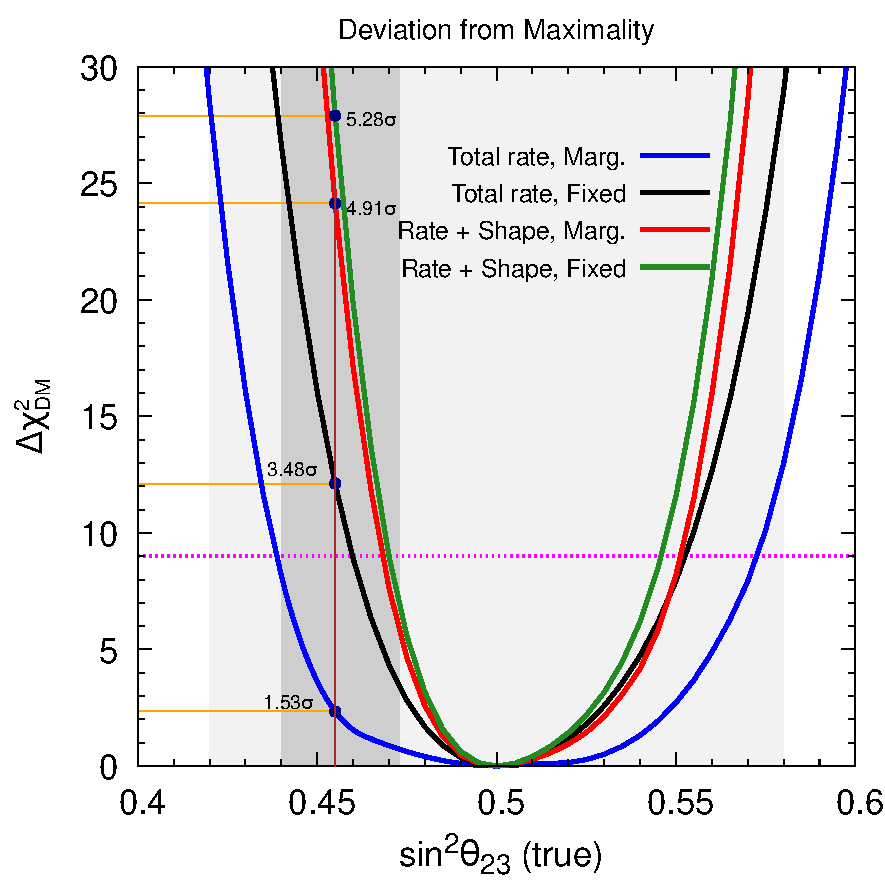
\includegraphics[width=0.7\textwidth]{./Figures/Chapter-4/New_All_channels_octant_deviation_marg_223.pdf}
	\caption{\footnotesize{Potential of DUNE to establish deviation from maximality as a function of true $\sin^2\theta_{23}$ assuming true NMO and $\delta_{\rm CP}$ (true) = 223$^\circ$ with the combined 3.5 years $\nu$ + 3.5 years $\bar{\nu}$ run. Blue (Black) curve shows the performance based on total event rates when $\Delta m^{2}_{31}$ and $\delta_{\mathrm{CP}}$ are marginalized (fixed) in the fit. Red (green) curve depicts the sensitivity based on rate + shape analysis when $\Delta m^{2}_{31}$ and $\delta_{\mathrm{CP}}$ are marginalized (fixed) in the fit. See text for details. The dark (light)-shaded grey area shows the currently allowed $1\sigma$ $(2\sigma)$ region in $\sin^{2}\theta_{23}$ as obtained in the global fit study~\cite{Capozzi:2021fjo} with the best-fit value of $\sin^{2}\theta_{23} = 0.455$ as shown by vertical brown line. The horizontal orange lines show the sensitivity (experessed in $\sigma = \sqrt{\Delta\chi^2_{\rm DM}}$) due to individual runs for the current best-fit value of $\sin^2\theta_{23}$. The capability of DUNE to establish non-maximal $\theta_{23}$ at 3$\sigma$ ($\Delta \chi^{2}_{\mathrm{DM}} = 9$) confidence level is shown by horizontal pink dotted line. For simplicity, we do not consider systematic uncertainties in this figure.}}
	\label{fig:8}
\end{figure}
%----------------------------------------------------

We now explore the benefit of spectral shape information in DUNE on top of total event rates in establishing deviation from maximality. In Fig.~\ref{fig:8}, we show $\Delta\chi^2_{\rm DM}$ as a function of true $\sin^2\theta_{23}$ for four cases. The blue and black curves are obtained based on total event rates, while the red and green curves show the sensitivity when we include the spectral shape information along with total event rates. For both total rate and rate + shape analyses, we estimate the sensitivities in the fixed-parameter and marginalized scenarios. In the fixed-parameter case, we keep all the oscillation parameters fixed at their best-fit values (see second column in Table~\ref{table:one}) in both data and fit, while in the marginalized case, we minimize over $\Delta m^2_{31}$ and $\delta_{\rm CP}$ in their current 3$\sigma$ ranges. This comparison between fixed-parameter (see black and green lines) and marginalized (see blue and red lines) scenarios enable us to see how much the sensitivity gets deteriorated due to the uncertainties on $\Delta m^2_{31}$ and $\delta_{\rm CP}$. While establishing non-maximal $\theta_{23}$, the bulk of the sensitivity stems from the disappearance channel (see Fig.~\ref{fig:7}) and the uncertainty on $\Delta m^{2}_{31}$ affects this channel more than $\delta_{\rm CP}$. This can be seen from the top panels of Figs.~\ref{fig:2} and~\ref{fig:3}, and Fig.~\ref{fig:6} also confirms that the impact of $\delta_{\rm CP}$ is minimal in establishing the deviation from maximality. At the same time, we expect that the upcoming medium-baseline reactor experiment JUNO will measure $\Delta m^{2}_{31}$ with utmost precision~\cite{EPS-HEP-Conference2021, JUNO:2015zny} before DUNE will start taking data. Therefore, it makes complete sense to analyze the potential of DUNE to establish non-maximal $\theta_{23}$ in the fixed-parameter scenario (see black and green lines). However, Fig.~\ref{fig:8} also reveals that the impact of uncertainty on $\Delta m^{2}_{31}$ in the marginalized case is substantialy reduced when we exploit the spectral shape information (see red line) $-$ thanks to the intense wide-band beam resulting into high-statitstics in disappearance mode and excellent energy resolution of LArTPC detector in DUNE~\cite{Friedland:2018vry, DeRomeri:2016qwo}. 

We see from Fig.~\ref{fig:8} that the ability of DUNE to exclude maximal mixing solution in the fit for $\sin^{2}\theta_{23}$ (true) = 0.455, gets significantly enhanced from 1.53$\sigma$ (see blue line) to 4.91$\sigma$ (see red line) when we include spectral shape information in the analysis. We see this improvement in the sensitivity because the impact of $\Delta m^2_{31} - \sin^2\theta_{23}$ degeneracy gets reduced substantially when we perform rate + shape analysis instead of using only total rates. As we already demonstrate before using Fig.~\ref{fig:5} in Sec.~\ref{events} that we can reduce the impact of this degeneracy because of the fact that energy bins on either side of the oscillation minimum in disappearance events show different behavior with respect to a change in the value of $\Delta m^2_{31}$. For this reason, in the fit, the test value of $\Delta m^2_{31}$ does not get deviate much from its central best-fit value. Nevertheless, we observe that even in the case of rate + shape analysis, the uncertainty in $\Delta m^{2}_{31}$ reduces the potential of DUNE to establish deviation from maximality for $\sin^{2}\theta_{23}$ (true) = 0.455 from 5.28$\sigma$ to 4.91$\sigma$ while going from fixed-parameter case to marginalized scenario. So, an ultra-precise measurement of $\Delta m^{2}_{31}$ in future will undoubtedly enhance DUNE's capability to establish deviation from maximal $\theta_{23}$. For the sake of simplicity, while addressing the advantage due to spectral analysis and the impact of marginalization over oscillation parameters in Fig.~\ref{fig:8},  we do not take into account the systematic uncertainties in the analysis.


%----------------------------------------------------
\subsubsection{Individual contributions from  neutrino and antineutrino runs}
%----------------------------------------------------

%----------------------------------------------------
\begin{figure}[htb!]
	\centering
	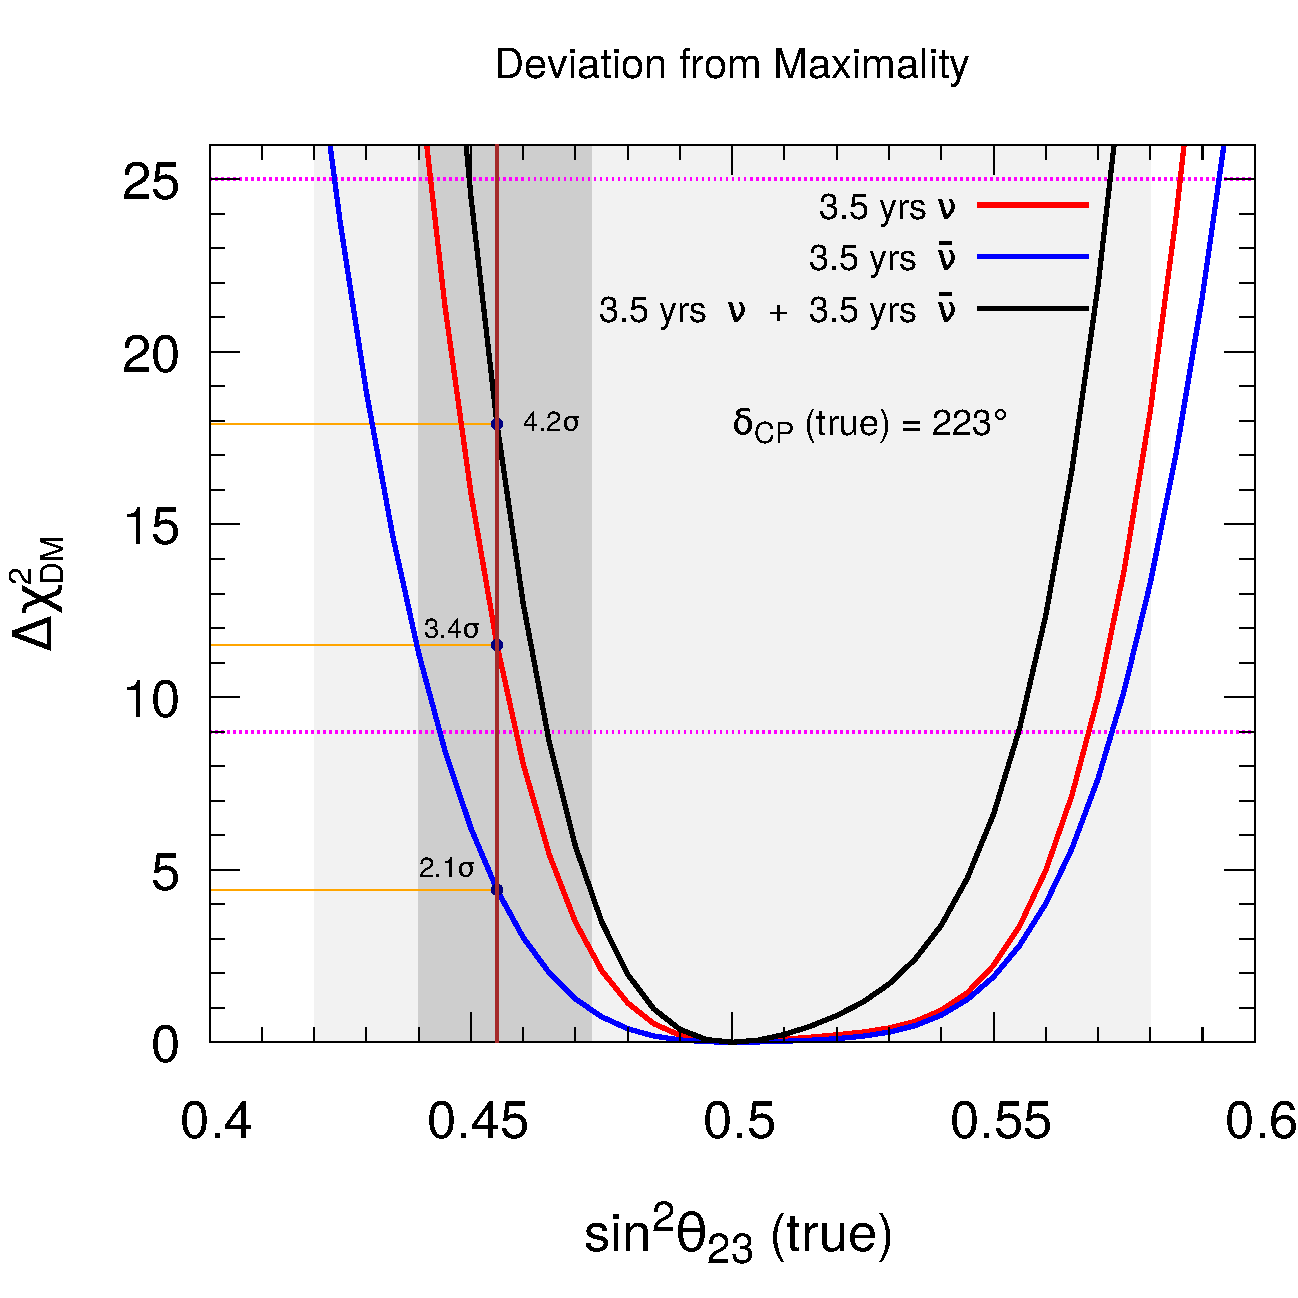
\includegraphics[width = 0.49\linewidth,height=0.51\linewidth]{./Figures/Chapter-4/Comb_C_Updated_different_channels_7yrs_octant_deviation_marg_223}
	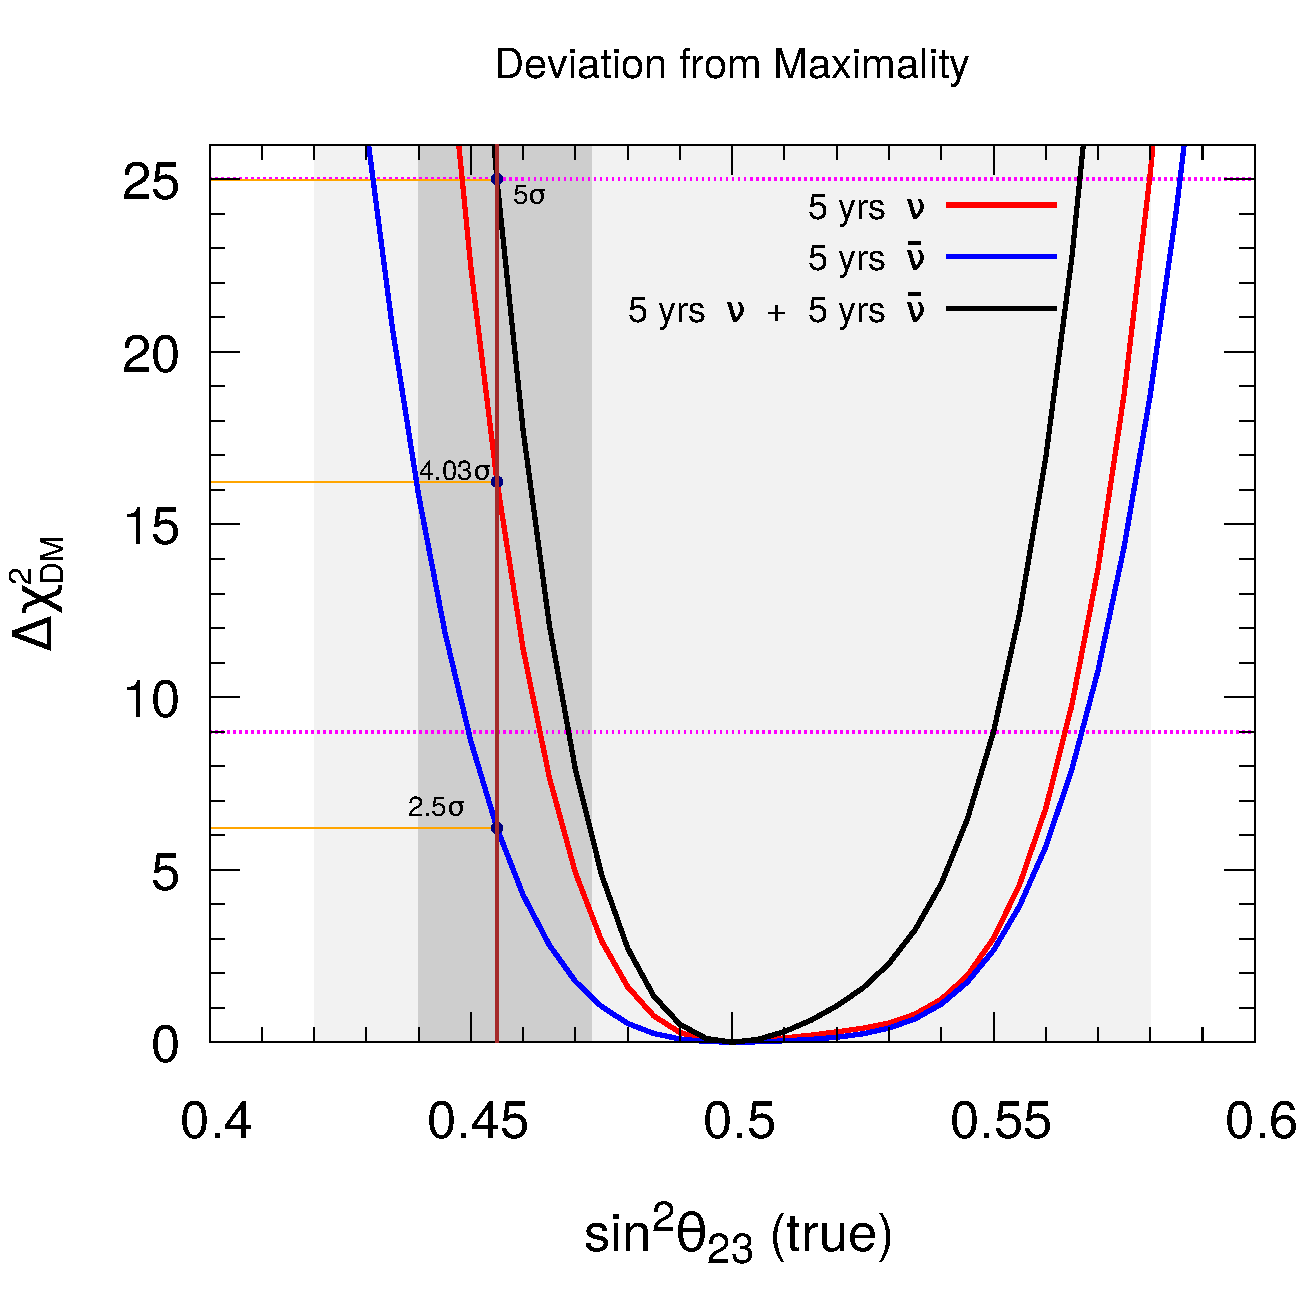
\includegraphics[width = 0.49\linewidth,height=0.51\linewidth]{./Figures/Chapter-4/Comb_C_Updated_different_channels_10yrs_octant_deviation_marg_223}
	\caption{\footnotesize{Potential of DUNE to establish the deviation from maximal $\theta_{23}$ as a function of true $\sin^2\theta_{23}$ assuming true NMO and $\delta_{\rm CP}\, \mathrm{(true)} = 223^\circ$. The red, blue, and black curves in the left (right) panel are drawn assuming 3.5 (5) years of neutrino run, 3.5 (5) years of antineutrino run, and the combined 7 (10) years of $\nu + \bar{\nu}$ run, respectively. In the fit, we marginalize over the current 3$\sigma$ range of $\Delta m^{2}_{31}$ and $\delta_{\rm CP}$, while keeping rest of the oscillation parameters fixed at their present best-fit values as shown in Table~\ref{table:one}. The dark (light)-shaded grey area shows the currently allowed $1\sigma$ $(2\sigma)$ region in $\sin^{2}\theta_{23}$ as obtained in the global fit study~\cite{Capozzi:2021fjo} assuming NMO with the best-fit value of $\sin^{2}\theta_{23} = 0.455$ as shown by vertical brown line. The horizontal orange lines show the sensitivity (experessed in $\sigma = \sqrt{\Delta\chi^2_{\rm DM}}$) due to individual runs for the current best-fit value of $\sin^2\theta_{23}$. The capability of DUNE to establish non-maximal $\theta_{23}$ at 3$\sigma$ ($\Delta \chi^{2}_{\mathrm{DM}} = 9$) and 5$\sigma$ ($\Delta \chi^{2}_{\mathrm{DM}} = 25$) confidence levels are shown by horizontal pink dotted lines.
	}}
	\label{fig:9}
\end{figure} 
%----------------------------------------------------

In Fig.~\ref{fig:9}, we demonstrate the capability of DUNE to establish non-maximal $\theta_{23}$ assuming true NMO and $\delta_{\rm CP}\, \mathrm{(true)} = 223^\circ$. The red, blue, and black curves in the left (right) panel are drawn assuming 3.5 (5) years of neutrino run, 3.5 (5) years of antineutrino run, and the combined 7 (10) years of $\nu + \bar{\nu}$ run, respectively. We observe that the sensitivity of DUNE to exclude maximal $\theta_{23}$ gets improved significantly when we combine the data from both neutrino and antineutrino modes (see black curves) as compared to the stand-alone neutrino (see red curves) or antineutrino (see blue curves) run. Mostly, the data from neutrino run contributes in the combined analysis due to their superior statistics. We notice from the left panel that a 2.1$\sigma$, 3.4$\sigma$, and 4.2$\sigma$ determination of non-maximal $\theta_{23}$ is possible in DUNE considering 3.5 years of $\bar{\nu}$ run, 3.5 years of $\nu$ run, and the combined 3.5 years $\nu$ + 3.5 years $\bar{\nu}$ run, respectively assuming the present best-fit values of $\sin^{2}\theta_{23}$ (0.455) and $\delta_{\rm CP}$ (223$^\circ$) as their true choices and with true NMO. In the right panel, the sensitivities get improved to 2.5$\sigma$, 4$\sigma$, and 5$\sigma$ with 5 years of $\bar{\nu}$ run, 5 years of $\nu$ run, and the combined 5 years $\nu$ + 5 years $\bar{\nu}$ run, respectively.

%----------------------------------------------------
\subsubsection{Performance as a function of exposure}
%----------------------------------------------------

%----------------------------------------------------
\begin{figure}[htb!]
	\centering
	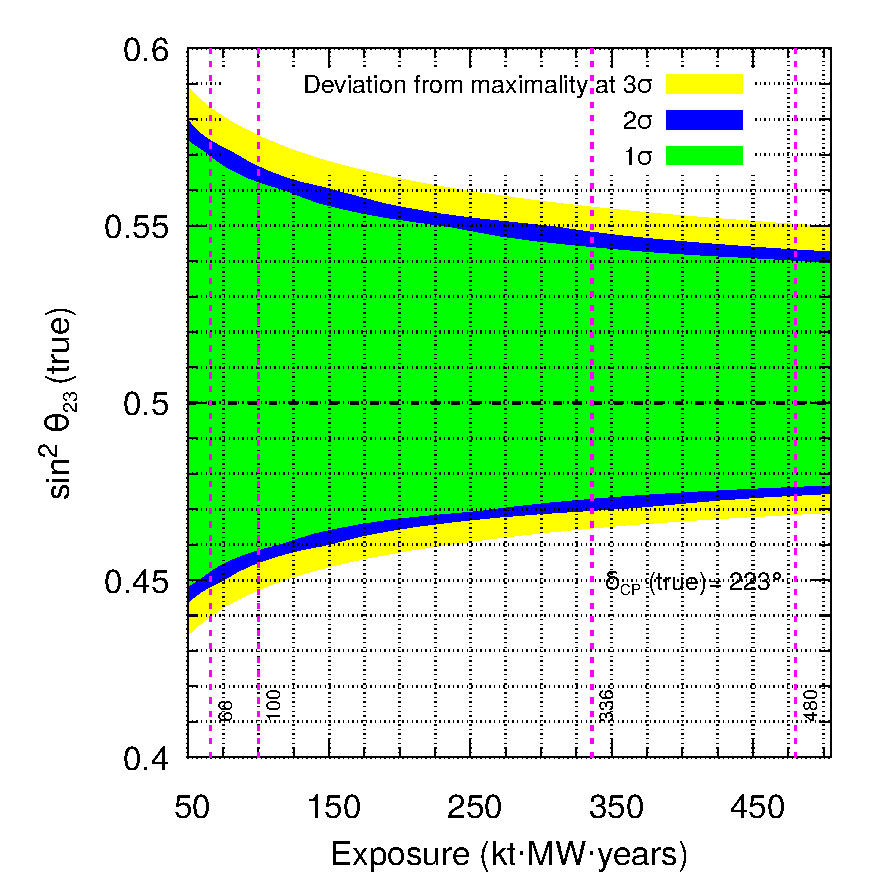
\includegraphics[width = 0.7\linewidth]{./Figures/Chapter-4/fixed_param.pdf}
	\caption{\footnotesize{The discovery of true values of non-maximal $\sin^{2}\theta_{23}$ as a function of exposure (kt$\cdot$MW$\cdot$years) at $3\sigma$ (yellow curves), $2\sigma$ (blue curves), and $1\sigma$ (green curves) confidence levels. For a given exposure, we assume equal run-time in both $\nu$ and $\bar{\nu}$ modes. We consider true NMO and $\delta_{\mathrm{CP}}$ (true) = 223$^{\circ}$. We marginalize over $\delta_{\mathrm{CP}}$ and $\Delta m^{2}_{31}$ in the fit in their allowed 3$\sigma$ ranges as given in Table~\ref{table:one}.}
	}
	\label{fig:10}
\end{figure}
%----------------------------------------------------

 The DUNE collaboration is planning to adopt an incremental approach where they will gradually increase the exposure by adding the new detector modules to their setup and will also upgrade the beam power from 1.2 MW to 2.4 MW after 6 years \cite{DUNE:2020jqi, DUNE:2021mtg} 
. This staging approach is well justified in light of the challenges that appear while operating a high-power superbeam and in constructing a massive underground 40 kt liquid argon detector. A nominal deployment plan is discussed in Ref. \cite{DUNE:2020jqi}, where the collaboration plans to start the experiment with two far detector (FD) modules having a total fiducial mass of 20 kt and with a beam power of 1.2 MW. After one year, they plan to add one more FD module of 10 kt fiducial mass and after two more years, they will add another 10 kt FD module to have the total fiducial mass of 40 kt. After operating the experiment for six years with a beam power of 1.2 MW, there is also a plan to upgrade the beam power to 2.4 MW \cite{DUNE:2020jqi}.

In Fig.~\ref{fig:10}, we exhibit the performance of DUNE to establish the possible deviation of true values of $\sin^{2}\theta_{23}$ from MM choice ($\sin^{2}\theta_{23}^{\mathrm{test}}$ = 0.5) in the fit as a function of exposure expressed in the units of kt$\cdot$MW$\cdot$years. We show the results at 3$\sigma$ (see yellow curves), 2$\sigma$(see blue curves), and 1$\sigma$ (see green curves) confidence levels assuming $\delta_{\mathrm{CP}}$ (true) = 223$^{\circ}$, and true NMO. While obtaining the results, we marginalize over $\delta_{\mathrm{CP}}$ and $\Delta m^{2}_{31}$ in their presently allowed 3$\sigma$ ranges as given in Table~\ref{table:one}. We see a significant improvement in the discovery of a non-maximal $\theta_{23}$ while increasing the exposure from 50 kt$\cdot$MW$\cdot$years to 100 kt$\cdot$MW$\cdot$years. In Fig.~\ref{fig:10} we show for the first time the true values of $\sin^{2}\theta_{23}$ that DUNE can distinguish from $\sin^{2}\theta_{23}^{\mathrm{test}}= 0.5$ using these exposures at various confidence levels (see dashed vertical lines). While further increasing the exposure from 100 kt$\cdot$MW$\cdot$years to 336kt$\cdot$MW$\cdot$years  which is our benchmark choice, we see a marginal increment in the performance. Note that we hardly see any improvement in the sensitivity if we increase the exposure further which suggest that the statistics is not a limiting factor anymore and any possible reduction in the systematic uncertainties may enhance the results further.

%%%%%%%%%%%%%%%%%%%%%%%%%%%%%%%%%%%%%%%%%%
\section{Summary and conclusions}
\label{conclusion}
%%%%%%%%%%%%%%%%%%%%%%%%%%%%%%%%%%%%%%%%%%

We have achieved remarkable precision on the solar ($\theta_{12}, \, \Delta m^{2}_{21}$) and atmospheric ($\theta_{23}, \, \Delta m^{2}_{31}$) oscillation parameters over the last few years. According to Ref.~\cite{Capozzi:2021fjo}, the current relative 1$\sigma$ errors on $\sin^{2}\theta_{12}, \, \Delta m^{2}_{21}, \, \sin^{2}\theta_{23}$, and $\Delta m^{2}_{31}$ are 4.5\%, 2.3\%, 6.7\%, and 1.1\%, respectively. The recent hints for normal mass ordering (at $\sim$ 2.5$\sigma$), as well as for lower octant $\theta_{23}$ ($\theta_{23} <$ 45$^{\circ}$) and for $\delta_{\mathrm{CP}}$ in the lower half-plane ($\sin \delta_{\mathrm{CP}} < 0$) signify major developments in the three-flavor neutrino oscillation paradigm. The high-precision measurement of $\theta_{13}$ from the Daya Bay reactor experiment and the possible complementarities between the recent Super-K Phase I-IV atmospheric data and the appearance and disappearance data from the ongoing long-baseline oscillation experiments - NO$\nu$A and T2K, play an important role in providing these crucial hints. An accurate measurement of $\theta_{23}$ and resolution of its octant (if $\theta_{23}$ turns out to be non-maximal) are crucial to transform these preliminary hints into 5$\sigma$ discoveries. A discovery of non-maximal $\theta_{23}$ at high confidence level will serve as a crucial input to the theories of neutrino masses and mixings and it will certainly be a major breakthrough in addressing the the age-old flavor problem. In this paper, we explore in detail the sensitivities of the upcoming high-precision long-baseline experiment DUNE to establish the possible deviation from maximal $\theta_{23}$ and to resolve its octant at high confidence level in light of the recent neutrino oscillation data. 

We start the paper by showing the possible correlations and degeneracies among the oscillation parameters $\sin^{2}\theta_{23}, \, \Delta
m^{2}_{31}$, and $\delta_{\mathrm{CP}}$ in the context of $\nu_{\mu} \rightarrow \nu_{\mu}$ disappearance channel and $\nu_{\mu} \rightarrow \nu_{e}$ appearance channel at the probability and event levels. We introduce for the first time, a bi-events plot in the plane of total neutrino and antineutrino disappearance events to demonstrate the impact of $\sin^{2}\theta_{23} - \Delta m^{2}_{31}$ degeneracy in establishing deviation from maximality. Next, we show how the spectral shape information in neutrino and antineutrino disappearance events can play an important role to resolve this degeneracy.

Using the latest simulation details of DUNE~\cite{DUNE:2021cuw}, we observe that a 3$\sigma$ (5$\sigma$) determination of non-maximal $\theta_{23}$ is possible in DUNE with an exposure of 336 kt$\cdot$MW$\cdot$years if the true value of $\sin^2\theta_{23} \lesssim 0.465~(0.450)$ or $\sin^2\theta_{23} \gtrsim 0.554~(0.572)$ for any value of true $\delta_{\mathrm{CP}}$ in the present 3$\sigma$ range and true NMO. DUNE can exclude the maximal mixing solution of $\theta_{23}$ at 4.2$\sigma$ (5$\sigma$) with a total 7 (10) years of run (equally divided in neutrino and antineutrino modes) assuming the present best-fit values of $\sin^{2}\theta_{23}$ (0.455) and $\delta_{\mathrm{CP}}$ (223$^{\circ}$) as their true choices with true NMO. The same can be enhanced to 6.5$\sigma$ (7.7$\sigma$) if we assume $\sin^{2}\theta_{23}$ (true) = 0.44, which is the current 1$\sigma$ lower bound. On the other hand, the sensitivity can be reduced to 2.07$\sigma$ (2.44$\sigma$) if $\sin^{2}\theta_{23}$ (true) turns out to be 0.473, which is the current 1$\sigma$ upper bound. 
 

We study the role that systematic uncertainties play in establishing  deviation from maximality by varying the normalization errors in both appearance and disappearance channels. We explore the contribution that each oscillation channel has on the sensitivity and show how performing a spectral analysis alleviates the possible reduction in sensitivity due to the marginalization over $\Delta m^2_{31}$ that is present when only total event rates are considered. We also explore the effect of exposure and the individual contributions from neutrino and antineutrino modes. We hope that this study serves as an important addition to several fundamental physics issues that can be explored by the high-precision long-baseline experiment DUNE and provides a boost to the physics reach of DUNE. For more details, see the reference \cite{Agarwalla:2021bzs}.


%%%%%%%%%%%%%%%%%%%%%%%%%%%%%%%%%%%%%%%%%%


%%%%%%%%%%%%%%%%%%%%%%%%%%%%
%%%%%%%%%%%%%%%%%%%%%%%%%%%%
%%%%%%%%%%%%%%%%%%%%%%%%%%%%

%\blankpage 
% %%%%%%%%%%%%%%%%%%%%%%%%%% Chapter-5 %%%%%%%%%%%%%%%%%%%%%%%%%%%%%%
%%%%%%%%%%%%%%%%%%%%%%%%%%%%%%% CHAPTER - 5 %%%%%%%%%%%%%%%%%%%%%%%%%%%%%%%%%%%%
\chapter{Improved precision on 2-3 oscillation parameters using the synergy between DUNE and T2HK}
\label{C5} 
%%%%%%%%%%%%%%%%%%%%%%%%%%%%%%%%%%%%%%%%%%%%%%%%%%%%%%%%%%%%%%%%%%%%%%%%%%%%%%%%
A high-precision measurement of $\Delta m^2_{31}$ and $\theta_{23}$ is inevitable to estimate the Earth's matter effect in long-baseline experiments which in turn plays an important role in addressing the issue of neutrino mass ordering and to measure the value of CP phase in $3\nu$ framework. After reviewing the results from the past and present experiments, and discussing the near-future sensitivities from the IceCube Upgrade and KM3NeT/ORCA, we study the expected improvements in the precision of 2-3 oscillation parameters that the next-generation long-baseline experiments, DUNE and T2HK, can bring either in isolation or combination. We highlight the relevance of the possible complementarities between these two experiments in obtaining the improved sensitivities in determining the deviation from maximal mixing of $\theta_{23}$, excluding the wrong-octant solution of $\theta_{23}$, and obtaining high precision on 2-3 oscillation parameters, as compared to their individual performances. We observe that for the current best-fit values of the oscillation parameters and assuming normal mass ordering (NMO), DUNE + T2HK can establish the non-maximal $\theta_{23}$ and exclude the wrong octant solution of $\theta_{23}$ at around 7$\sigma$ C.L. with their nominal exposures. We find that DUNE + T2HK can improve the current relative 1$\sigma$ precision on $\sin^{2}\theta_{23}~(\Delta m^{2}_{31})$  by a factor of 7 (5) assuming NMO. Also, we notice that with less than half of their nominal exposures, the combination of DUNE and T2HK can achieve the sensitivities that are expected from these individual experiments using their full exposures. We also portray how the synergy between DUNE and T2HK can provide better constraints on ($\sin^2\theta_{23}$ - $\delta_{\mathrm{CP}}$) plane as compared to their individual reach.
Current oscillation experiments in the three-neutrino paradigm depict potent complementarity. The Solar experiment's precision measurements of solar mixing angle have been combined with KamLAND's ability to determine solar mass splitting well, enabling their synergy to be utilized in the neutrino community for a very long time. The combination of these data and those from long-baseline (LBL) accelerator and atmospheric neutrinos represents the minimal dataset for the characterization of oscillation parameters. The unprecedented precision obtained on the reactor mixing angle ($\theta_{13}$) from short-baseline reactor data like Daya Bay~\cite{DayaBay:2022orm} has further alleviated the uncertainty in the measurements of other unknowns like $\theta_{23},\, \delta_{\mathrm{CP}}$, and the sign of $\Delta m^{2}_{31}$ indirectly by reducing the correlations. The atmospheric neutrino data, when complemented with the long-baseline data, allows us to gain valuable insight into the atmospheric parameters. For example, Super-K, with its extensive statistics, can impose strict constraints on the measurements of $\theta_{23}$, while MINOS/MINOS$+$, benefiting from a precisely known $L/E$ ratio, can offer more accurate measurements of the atmospheric mass splitting, as illustrated in figure~\ref{fig:moneyplot}. In this context, recently, the Super-K experiment has enhanced its precision on atmospheric neutrino oscillation parameters by using the number of tagged neutrons to enhance the separation between neutrino and antineutrino events, improving the efficiency to classify the multi-ring events using a boosted decision tree algorithm, and adding 48\% exposure by analyzing events from an expanded fiducial volume and from 1186 additional live-days, including the data which were collected after a major refurbishment of the detector in 2018~\cite{Super-Kamiokande:2023ahc}.

The presently running accelerators~\cite{Ali:2022mrp,Catano-Mur:2022kyq} and atmospheric experiments~\cite{sk,IceCube:2019dyb} along with the high-precision measurements from reactors~\cite{DayaBay:2018yms,Seo:2019shs} have helped to achieve the current relative 1$\sigma$ precision of about 1.1\% and 6.7\% in the atmospheric parameters: $\Delta m^{2}_{31}$ and $\sin^2\theta_{23}$, respectively~\cite{Capozzi:2021fjo}. The upcoming medium-baseline reactor oscillation experiment JUNO~\cite{JUNO:2022mxj} is expected to achieve considerable improvement in the precision of atmospheric mass-squared difference $\Delta m^2_{32}$ as compared to the current precision from Daya Bay~\cite{DayaBay:2022orm} reactor experiment, as can be seen from figure~\ref{fig:moneyplot}. The DeepCore array consisting of 8 dedicated strings with denser spacing in the central region of IceCube has enabled the detection and reconstruction of atmospheric neutrinos with energies as low as a few GeV, providing high-precision measurements of 2-3 oscillation parameters. Using convolutional neural networks with 9.3 years of data, the IceCube DeepCore has provided a new high-precision measurements of $\Delta m^{2}_{32} = 2.40^{+0.05}_{-0.04} \times 10^{-3}$  eV$^{2}$ and $\sin^{2}\theta_{23}= 0.54^{+0.04}_{-0.03}$~\cite{IceCube:2024xjj} assuming normal mass ordering (NMO), which are compatible and complementary with the existing measurements from the long-baseline experiments. A new extension of IceCube, namely the IceCube Upgrade to be deployed in the polar session of 2025/26 with seven new strings in the central region of DeepCore detector and an energy threshold of around 1 GeV is expected to improve the precision of 2-3 oscillation parameters by (20-30)\%~\cite{IceCube:2023ins}. In ref.~\cite{IceCube-Gen2:2019fet}, the combined sensitivity of the future JUNO, IceCube Upgrade, and PINGU data was estimated to resolve the pressing issue of neutrino mass ordering. The under-construction water Cherenkov neutrino detector KM3NeT/ORCA also has the potential to shed light on neutrino mass ordering and 2-3 oscillation parameters~\cite{KM3NeT:2021ozk}. In fact, recently, they announced their measurements of 2-3 oscillation parameters using an initial configuration with 6-detection units of photo-sensors corresponding to an exposure of 433 kt$\cdot$yr, collected in 510 days of data taking~\cite{KM3NeT:2024ecf}. They reveal a best-fit of $\sin^{2}\theta_{23}= 0.51$ and $\Delta m^{2}_{31} = 2.14 \times 10^{-3}$  eV$^{2}$ with their initial configuration, referred to as ORCA6. Further, in the Neutrino 2024 conference, the KM3NeT/ORCA collaboration showed slightly improved measurements of 2-3 oscillation parameters using an updated exposure of 715 kt$\cdot$yr~\cite{coelho_orca}. In ref.~\cite{KM3NeT:2021rkn}, a combined analysis of the prospective JUNO and KM3NeT/ORCA data was performed to determine the correct neutrino mass ordering.

%===================================
\begin{figure}[t!]
	\centering
	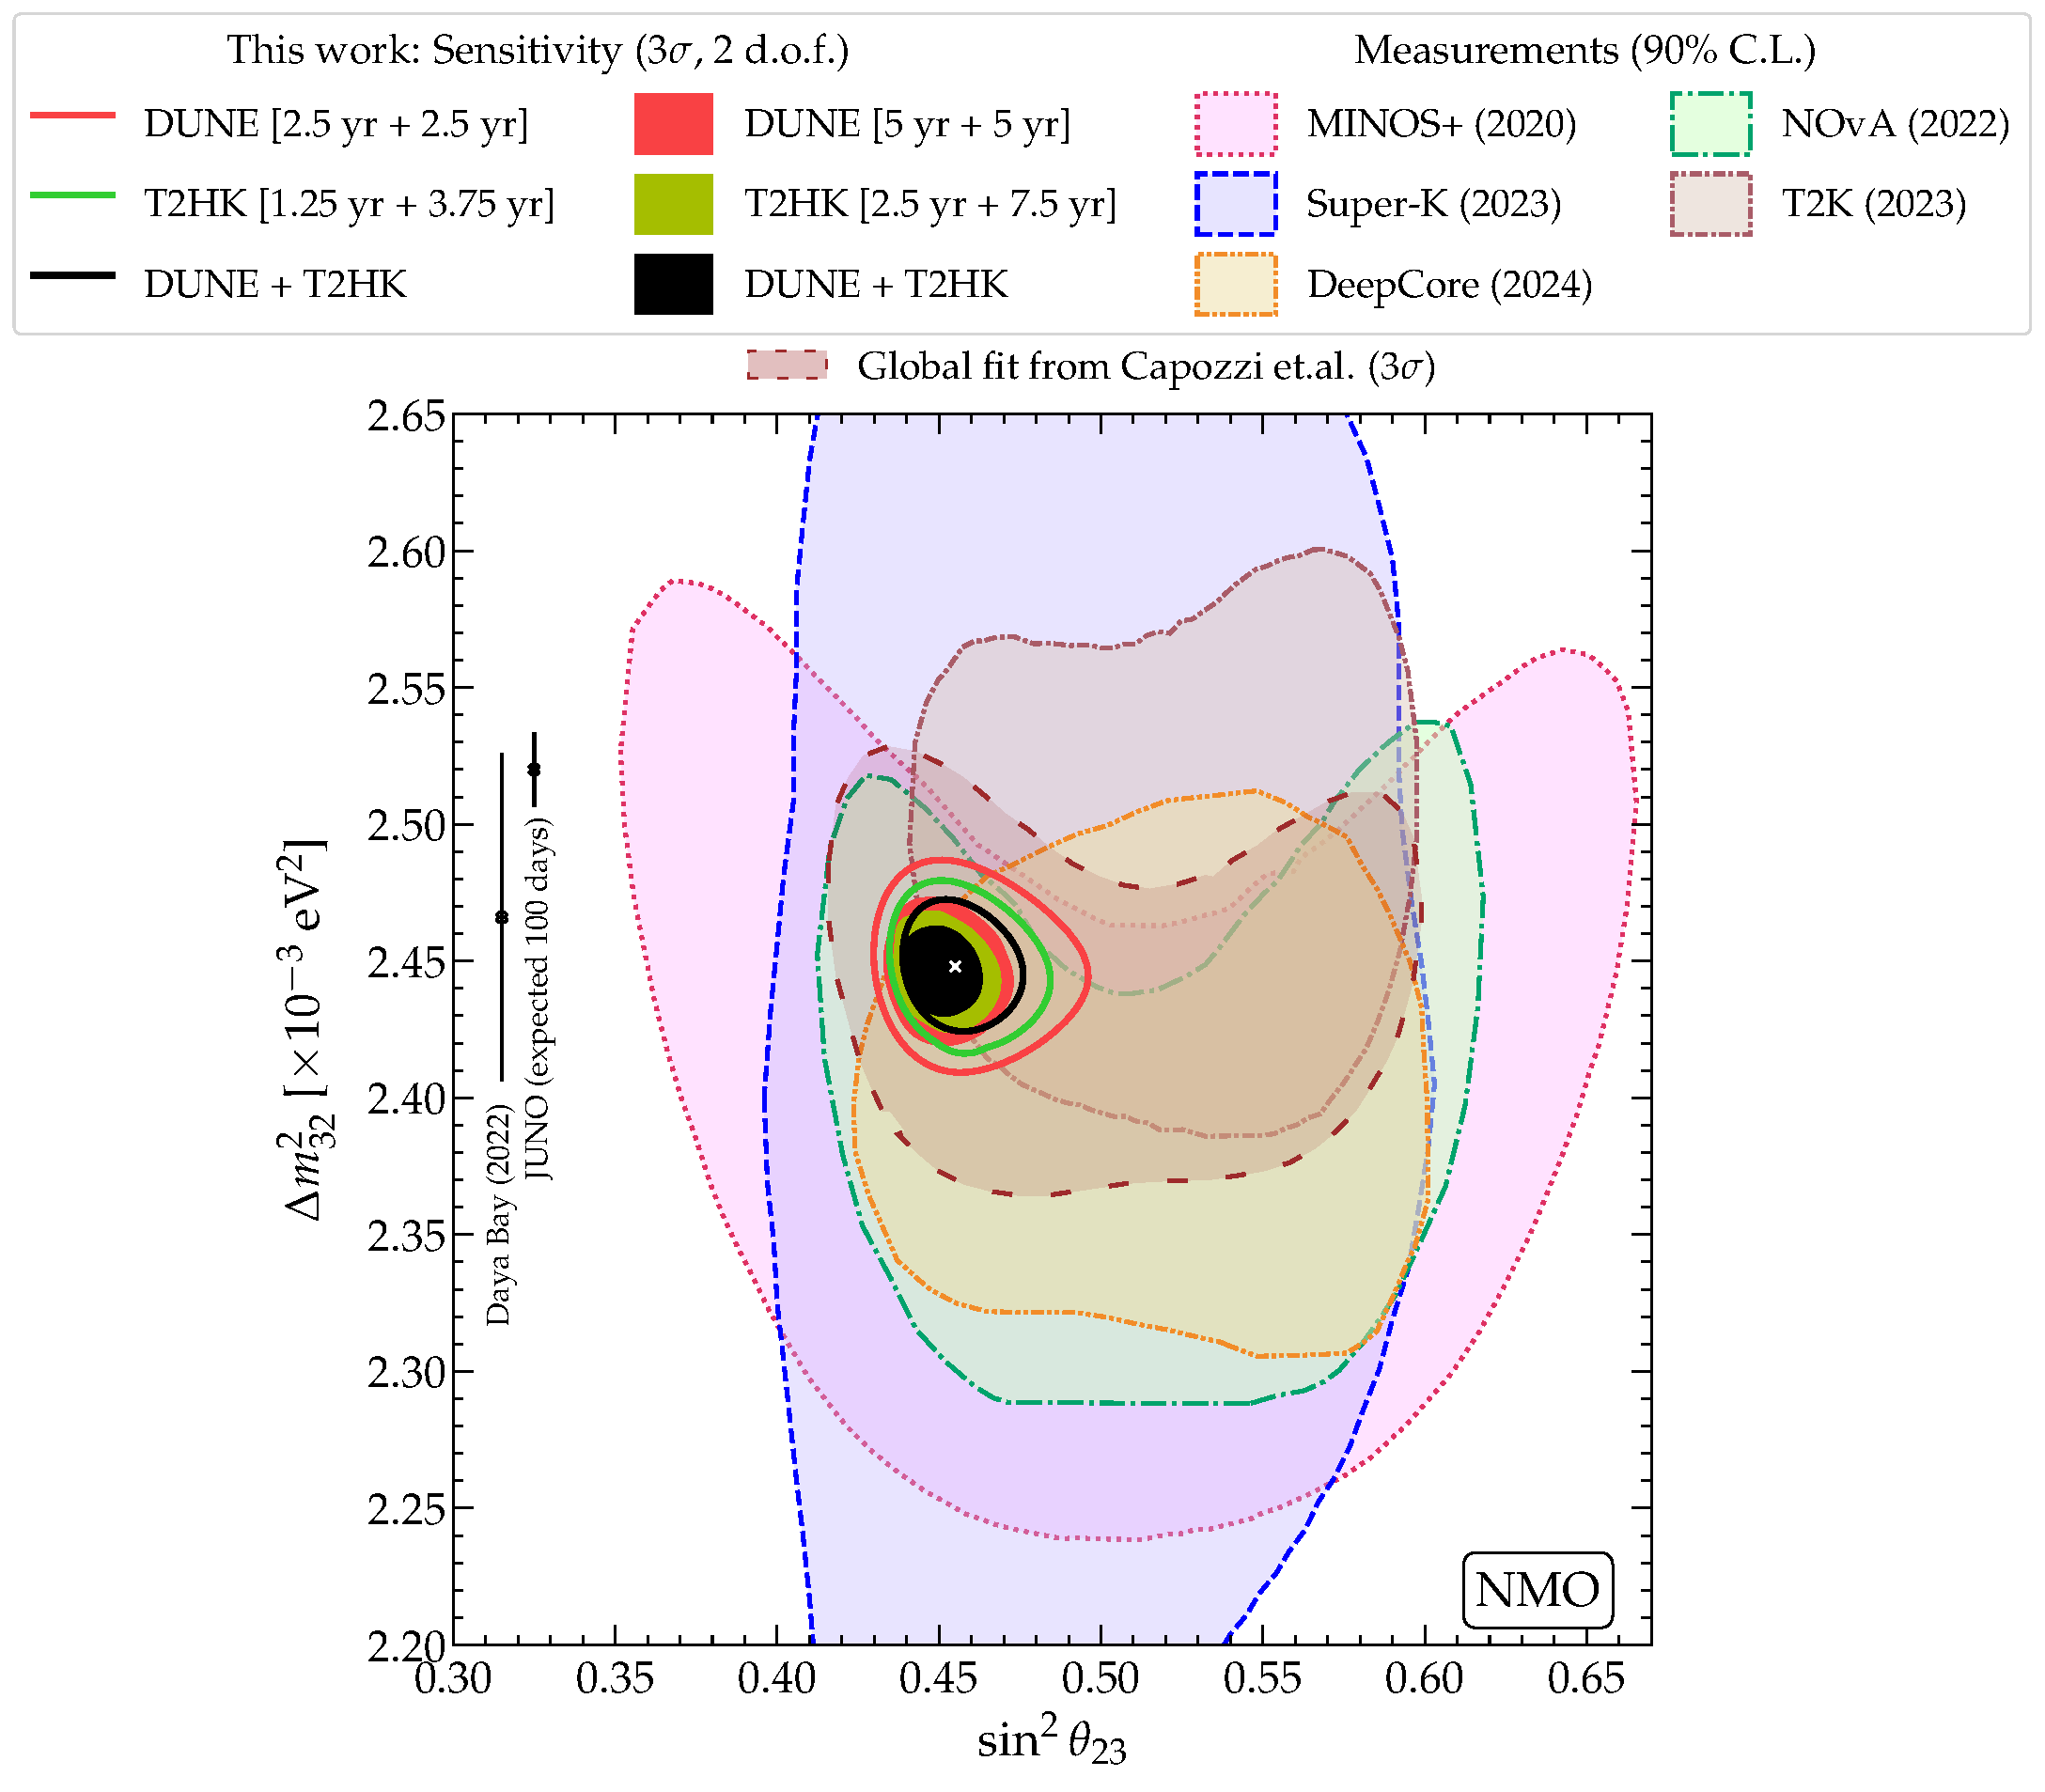
\includegraphics[width=\linewidth]{./Figures/Chapter-5/th23_Dm31}
	\caption{\footnotesize{Allowed ranges at 3$\sigma$ (2 d.o.f.) in the atmospheric mixing parameters, $\sin^{2}\theta_{23}$ and $\Delta m^{2}_{32}$, using DUNE, T2HK, and DUNE + T2HK. DUNE is expected to have an exposure of 480 kt$\cdot$MW$\cdot$yr and T2HK, an exposure of 2431 kt$\cdot$MW$\cdot$yr. We assume DUNE (T2HK) running for 5 (2.5) yr in $\nu$ and 5 (7.5) yr in $\bar{\nu}$ mode while estimating nominal exposure. We also depict the allowed ranges for the same when only half of the total projected exposure is considered (DUNE: [2.5 yr in $\nu$ + 2.5 yr in $\bar{\nu}$], T2HK: [1.25 yr in $\nu$ + 3.75 yr in $\bar{\nu}$]). Existing allowed ranges are from: Super-Kamiokande~\cite{Super-Kamiokande:2023ahc}, Tokai-to-Kamioka (T2K)~\cite{T2K:2023smv}, NuMI Off-Axis $\nu_{e}$ Appearance (NO$\nu$A)~\cite{NOvA:2021nfi}, Main injector neutrino oscillation search (MINOS+)~\cite{MINOS:2020llm}, and IceCube DeepCore~\cite{IceCube:2024xjj,Yu:2023tmw} at 90\% C.L. We also show existing (expected) bounds on $\Delta m^{2}_{32}$ from Daya Bay~\cite{DayaBay:2022orm} 
 (Jiangmen Underground Neutrino Observatory; JUNO ~\cite{JUNO:2022mxj}).  To have a complete picture, we also show the present global fit, following Ref.~\cite{Capozzi:2021fjo} at 3$\sigma$ (1dof). \textit{Our projected allowed ranges improve from the existing bounds by manifold.} See section~\ref{appendix1} for a detailed discussion.Further, figure~\ref{fig:allowed-ranges-nmo} elaborates on the importance of both neutrino and antineutrino modes in this sensitivity separately. Also, see figure~\ref{fig:appendix-allowed-ranges-nmo} for a few additional sensitivity curves.}} 
 \label{fig:moneyplot}
 \end{figure}
%=====================================
The present hints of non-maximal $\theta_{23}$ from the global oscillation data~\cite{Capozzi:2021fjo,deSalas:2020pgw,Esteban:2020cvm,NuFIT} give rise to two probable solutions: $\theta_{23} < 45^{\circ}$ or the lower octant solutions (LO) and $\theta_{23} > 45^{\circ}$ or the higher octant solutions (HO)~\cite{Fogli:1996pv, Barger:2001yr, Minakata:2002qi, Minakata:2004pg, Hiraide:2006vh}. Prior to delving into the determination of the correct octant, it is imperative to eliminate the possibility of maximal mixing with a high level of confidence. This investigation was undertaken earlier, taking into account the forthcoming DUNE (Deep Underground Neutrino Experiment)~\cite{Agarwalla:2021bzs}. In this study, we explore the synergies between the two prominent upcoming neutrino experiments: DUNE~\cite{DUNE:2020jqi, DUNE:2020ypp}, designed to receive a wide-band on-axis neutrino beam traversing a distance of around 1300 km with substantial Earth matter effect, and T2HK (Tokai to Hyper-Kamiokande)~\cite{Hyper-KamiokandeProto-:2015xww, Hyper-Kamiokande:2018ofw}, which proposes the use of a narrow-band off-axis neutrino beam with a baseline of 295 km having minimal Earth matter effect. We investigate how the collaborative synergy of these setups enhances their individual sensitivities. Additionally, we assess the expected sensitivities of currently running long-baseline experiments: T2K (Tokai to Kamioka)~\cite{T2K:2011qtm} and NO$\nu$A (NuMI Off-Axis $\nu_{e}$ Appearance)~\cite{NOvA:2007rmc}, considering their full projected exposures. Our findings indicate that the combined DUNE + T2HK configuration can detect a departure from maximal $\theta_{23}$ with exceptional significance. Moreover, their complementarity turns out to be essential for achieving degeneracy-free and significantly precise measurements of both $\sin^2\theta_{23}$ and $\Delta m^{2}_{31}$.

As mentioned before, figure~\ref{fig:moneyplot} shows a part of our main results exhibiting the expected precision in 2-3 oscillation parameters: $\sin^{2}\theta_{23}$ and $\Delta m^{2}_{32}$ at 3$\sigma$ confidence level (C.L.) using the projected full and half exposures of standalone DUNE and T2HK, and their combination (DUNE + T2HK). To have a better comparison, we also include the currently allowed regions from the ongoing (T2K, NO$\nu$A, IceCube DeepCore, Super-Kamiokande), completed (Daya Bay and MINOS+), and upcoming (JUNO) experiments at 90\% C.L. assuming NMO. The details of these experiments (such as exposures, runtime, and current status) and the best-fit values of the oscillation parameters obtained from them are given in table~\ref{tab:other-experiments}. In figure~\ref{fig:moneyplot}, we also show the allowed region from the global fit of all the available oscillation data following Ref.~\cite{Capozzi:2021fjo} at 3$\sigma$, assuming NMO. More details related to this figure can be found in section~\ref{appendix2}. Note that in figure~\ref{fig:moneyplot}, we compare the sensitivities of various experiments in terms of $\Delta m^{2}_{32}$ (see the y-axis). However, we present all our results in terms of $\Delta m^{2}_{31}$ in the present manuscript. 
%%%%%%%%%%%%%%%%%%%%%%%%%%%%%%%%%%%%%%%%%%
\begin{table}[htb!]
 \begin{tabular}{ | c | c | c | c | c | c|}
 \hline
 \multirow{3}{*}{Experiment}
 & \multicolumn{2}{c|}{Best-fit} &  \multirow{3}{*}{Exposure} &  \multirow{3}{*}{Span} &  \multirow{3}{*}{Status}\\ 
 \cline{2-3}
 &  \multirow{2}{*}{$\sin^{2}\theta_{23}$} & $\Delta m^{2}_{32}$ &    &  &\\
  & & $[10^{-3}] ~\text{eV}^2$ &   & &\\
  \hline
\multirow{3}{*}{T2K~\cite{T2K:2023smv}} & \multirow{3}{*}{0.56} & \multirow{3}{*}{2.49} &  P.O.T. & \multirow{3}{*}{2010 - 2020} & \multirow{3}{*}{Ongoing}\\
%\cline{4}
& & & $16.3 \times 10^{20}$ ($\nu$)  & & \\
& & & $19.7 \times 10^{20}$ ($\bar{\nu}$)  & & \\
\hline
\multirow{3}{*}{NO$\nu$A~\cite{NOvA:2021nfi}} & \multirow{3}{*}{0.57} & \multirow{3}{*}{2.41} & P.O.T. &  & \multirow{3}{*}{Ongoing} \\
& & & $13.6 \times 10^{20}$ ($\nu$) & 2016 - 2019 & \\
& & & $12.5 \times 10^{20}$ ($\bar{\nu}$) & 2014 - 2020 & \\
\hline
MINOS/ & \multirow{2}{*}{0.43} & \multirow{2}{*}{2.4} & $23.76 \times 10^{20}$ P.O.T. & 2005 - 2016 & \multirow{2}{*}{Completed}\\
MINOS$+$~\cite{MINOS:2020llm}& & & 60.75 kt$\cdot$yr & 2011 - 2016 & \\
\hline
Super-K & \multirow{2}{*}{0.49} & \multirow{2}{*}{2.4} & \multirow{2}{*}{484.2 kt$\cdot$yr}  & \multirow{2}{*}{1996 - 2020} & \multirow{2}{*}{Ongoing}\\ 
(I - V)~\cite{Super-Kamiokande:2023ahc} & & & & & \\
\hline
IceCube- & \multirow{2}{*}{0.54} & \multirow{2}{*}{2.4} & \multirow{2}{*}{9.3 yr} & \multirow{2}{*}{2012 - 2021} & \multirow{2}{*}{Ongoing}\\
DeepCore~\cite{IceCube:2024xjj} & & & & & \\
\hline
Daya Bay~\cite{DayaBay:2022orm} & - & 2.466 & 3158 live days & 2011 - 2020 & Completed\\
\hline
JUNO~\cite{JUNO:2022mxj} & - & 2.52 & 6 yr & - & Upcoming\\
\hline
 \end{tabular}
 \caption{\footnotesize{Existing and expected best-fit values, collected exposure, runtime, and the present status of atmospheric parameters using long-baseline, atmospheric, and reactor experiments. Collected exposure is expressed in protons on target (P.O.T.) for long-baseline experiments and in kt$\cdot$yr for atmospheric experiments. For certain cases, we give the number of years of data collection. Using these details, currently allowed regions in the $\sin^{2}\theta_{23}$ and $\Delta m^{2}_{32}$ plane is shown in figure~\ref{fig:moneyplot}. 
 }}
 \label{tab:other-experiments}
\end{table}
%%%%%%%%%%%%%%%%%%%%%%%%%%%%%%%%%%%%%%%%%%

The other main results include sensitivity towards deviation from maximal $\sin^{2}\theta_{23}$, exclusion of wrong octant solutions of $\sin^{2}\theta_{23}$, and precision on atmospheric parameters, studied as a function of exposure. We find that the \textit{complementarity between DUNE and T2HK plays a crucial role in reducing the dependency on large projected exposures of standalone experiments by manifold. Furthermore, the synergy between them helps in removing the degeneracies introduced by the individual setups, if any. } \\

The roadmap of this chapter is laid out as follows. In section \ref{sec:events}, we summarize the characteristic features of DUNE and T2HK and discuss the effect of wrong-sign contaminations and variation of 2-3 oscillation parameters on the total event statistics and event spectra, respectively. Next, section \ref{sec:results}, elaborates on our results and discussions. We compute the sensitivities in establishing deviation from maximal $\sin^2\theta_{23}$, exclusion of wrong octant solutions of $\sin^2\theta_{23}$, and the precision of $\sin^2\theta_{23}$ and $\Delta m^2_{31}$, using DUNE and T2HK in both isolation and combination. We also analyze the effect of scaled exposure on the above-mentioned sensitivity studies. Then, section \ref{sec:contour} shows projected allowed ranges in $(\sin^2\theta_{23}-\delta_{\mathrm{CP}})$ plane, using half and full exposures in DUNE, T2HK, and their combination. Finally, in section \ref{conclusion}, we summarize our findings and provide concluding remarks. While section \ref{appendix1} comprehends the individual roles of $\nu$ and $\bar{\nu}$ modes, using  DUNE, T2HK, and DUNE + T2HK in $(\sin^2\theta_{23}-\delta_{\mathrm{CP}})$ plane; section \ref{appendix2} depicts past, present, and upcoming projected sensitivities in $(\sin^2\theta_{23}-\delta_{\mathrm{CP}})$ plane.

%======================================
\section{Experimental details and total event rates}
\label{sec:events}
%======================================

We initiate our discussion by comparing and contrasting the two upcoming long-baseline experiments under consideration: DUNE and T2HK. Following this, we compute the expected total appearance and disappearance event rates in both the $\nu$ and the $\bar{\nu}$ modes for the presently allowed 3$\sigma$ ranges in $\theta_{23}$ and $\Delta m^{2}_{31}$~\cite{Capozzi:2021fjo} using GLoBES~\cite{Huber:2004ka, Huber:2007ji}. Since the far detectors in both DUNE and T2HK are unable to differentiate between neutrinos and antineutrinos, we also discuss the effect of ``wrong-sign'' contamination, which is considered a part of the signal in both the experiments.
%  
%----------------------------------------------------------------------------
\subsection{Complementarities between DUNE and T2HK}
\label{sec:2a}
%----------------------------------------------------------------------------
 
DUNE  and T2HK  are two promising long-baseline experiments expected to achieve significant aspects of physics beyond the three-neutrino oscillations. We consider a single-phase state-of-the-art 40 kt Liquid Argon Time Projection Chamber (LArTPC) far detector in DUNE and a 187 kt Water Cherenkov far detector in T2HK as referred in their cumulative design reports, respectively~\cite{DUNE:2021tad, Hyper-Kamiokande:2016srs}. The neutrino flux in DUNE is expected to be wide-band on-axis, ranging from a few hundreds of MeV to a few tens of GeV, peaking at 2.5 GeV. This wide-band nature enables DUNE access to an envelope of various $L/E$ ratios, where $L$ corresponds to the distance that neutrino travels from source to detector and $E$ refers to the neutrino beam energy. Contrastingly, T2HK is expected to use a 2.5$^{\circ}$ off-axis J-PARC neutrino beam, the flux expected to peak at 0.6 GeV. The higher baseline in DUNE (1285 km; from Fermilab to South Dakota) ensures sufficient matter effect, while the relatively shorter baseline in T2HK (295 km; from J-PARC proton synchrotron facility to Hyper-Kamiokande) secures better precision in measurements of the intrinsic CP phase. The line-averaged constant Earth matter density ($\rho_{\mathrm{avg}}$) in DUNE is considered to be 2.848 g/cm$^3$, while in T2HK, it is taken as 2.8 g/cm$^3$. In DUNE, we consider 2\% detector systematic uncertainties in the appearance and  5\% in disappearance signal events following ref.~\cite{DUNE:2021cuw}. The binned events in T2HK have been matched with ref.~\cite{Hyper-Kamiokande:2016srs}, considering 5\% in appearance and 3.5\% in disappearance systematic uncertainties in signal events. Recently, apart from considering 5\% of conservative systematic uncertainties in appearance events, the T2HK collaboration is expecting to improve this uncertainty to about 2.7\% by the time they start taking their data in real-time~\cite{Munteanu:2022zla}. Thus we compare our results with both of these choices in figure~\ref{fig:octant exclusion}. For the runtime in DUNE, they expect to witness a balanced run between neutrino and antineutrino modes following [5 years in $\nu$ + 5 years in $\bar{\nu}$], T2HK aims instead to have an almost equal number of events in both the modes, thus following the 1:3 ratio of [2.5 years in $\nu$  + 7.5 years in $\bar{\nu}$]. Owing to the much higher detector fiducial mass, T2HK expects to accumulate about $2.7 \times 10^{22}$ P.O.T. in total ten years, providing a benchmark exposure of 2431 kt$\cdot$MW$\cdot$yr, while DUNE envisions a P.O.T. of around $1.1 \times 10^{21}$ per year with a benchmark exposure of 480 kt$\cdot$MW$\cdot$yr. In table~\ref{table:one}, we mention our assumed benchmark values and the ranges, which are taken from ref.~\cite{Capozzi:2021fjo}.

As the far detector deployment schedule and beam power scenarios are both subject to change, the results shown in this work are consistently given in terms of exposure in units of kt$\cdot$MW$\cdot$yr, which is agnostic to the exact staging scenario but can easily be expressed in terms of experiment years for any desired scenario. For having a complete summary, we present the sensitivity studies of DUNE and T2HK along with the full potential of ongoing long-baseline experiments: T2K and NO$\nu$A. We present our findings using the entire projected exposures of $84.4$ kt$\cdot$MW$\cdot$yr, generating $7.8 \times 10^{21}$ P.O.T. with a 750 kW beam power, evenly distributed between neutrino and antineutrino modes, as outlined in the ongoing long-baseline experiment T2K~\cite{T2K:2014xyt}. Additionally, we conduct simulations for the full projected exposure of NO$\nu$A, amounting to 58.8 kt$\cdot$MW$\cdot$yr and producing $3.6 \times 10^{21}$ P.O.T. with a 700 kW beam power, equally divided between neutrino and antineutrino modes, in accordance with ref.~\cite{NOvA:2007rmc, Patterson:2012zs}. In both experiments, we assume uncorrelated 5\% and 10\% systematic errors on signal and background events for both appearance and disappearance event rates.
%
%----------------------------------------------
\begin{table}[t!]
\centering
\resizebox{\columnwidth}{!}{%
\begin{tabular}{|c|c|c|c|c|c|c|}
\hline 
\multirow{2}{*}{\textbf{Parameter}} & $\Delta m^2_{21}/10^{-5}$ & \multirow{2}{*}{$\sin^{2}\theta_{12}/10^{-1}$} & \multirow{2}{*}{$\sin^{2}\theta_{13}/10^{-2}$} & \multirow{2}{*}{$\sin^2\theta_{23}/10^{-1}$} & $\Delta m^2_{31}/10^{-3}$  & $\delta_{\text{CP}}$ \\
				&($\mathrm{eV^{2}}$) & & & &($\mathrm{eV^{2}}$)&($^\circ$)\\
				\hline 
				{\textbf{Benchmark}} & $7.36$ & $3.03$ & $2.23$ & $4.55$ & $2.522$ & $223$\\
				%\cline{2-7}
    \hline
				\textbf{$3\sigma$ range}& - & - & - & 4.16 - 5.99 & 2.436 - 2.605 & 139 - 355\\
					\hline 
			\end{tabular}
			}
			\caption{\footnotesize{The benchmark values of the oscillation parameters and their corresponding 3$\sigma$ allowed ranges considered in our study assuming normal mass ordering (NMO) following the ref.~\cite{Capozzi:2021fjo}.}}
			\label{table:one}
	\end{table}
%----------------------------------------

%----------------------------------------
\subsection{Events due to wrong-sign contamination }
\label{sec:2c}
%-----------------------------------------
\begin{table}[t!]
 \centering
 \begin{tabular}{ | c  *{6}{>{\centering\arraybackslash}p{2.2cm} |}}
 \hline
 \multicolumn{2}{|c|}{\multirow{3}{*}{Experiment}}
 & \multicolumn{4}{c|}{Number of events (NMO)} \\
 \cline{3-6}
          & & \multicolumn{2}{c|}{Appearance} 
          & \multicolumn{2}{c|}{Disappearance} \\
          \cline{3-6}
          & & $\nu$ mode & $\bar{\nu}$ mode & $\nu$ mode & $\bar{\nu}$ mode \\
 \hline
  \multirow{4}{*}{DUNE} & w/  & \multirow{2}{*}{1592} & \multirow{2}{*}{294} & \multirow{2}{*}{14598} & \multirow{2}{*}{8270} \\
                         & wrong-sign    &  &  &  & \\            
                      & w/o    & \multirow{2}{*}{1576} & \multirow{2}{*}{186} & \multirow{2}{*}{13413} & \multirow{2}{*}{4360}   \\
                 & wrong-sign &  &  & &  \\
 \hline
 \multirow{4}{*}{T2HK} & w/  & \multirow{2}{*}{1598} & \multirow{2}{*}{919} & \multirow{2}{*}{10064} & \multirow{2}{*}{13949} \\
                 &  wrong-sign   & &  & & \\
                       & w/o    & \multirow{2}{*}{1588}  & \multirow{2}{*}{755} & \multirow{2}{*}{9487} & \multirow{2}{*}{8985}   \\
                       &  wrong-sign    &  & & &  \\
 \hline
 \end{tabular}
 \caption{\footnotesize{Total (Signal) appearance and disappearance event rates in DUNE and T2HK assuming 480 kt$\cdot$MW$\cdot$yr and 2431 kt$\cdot$MW$\cdot$yr of exposure, respectively.  We fix the values of the standard mixing parameters to their benchmark values from~\cite{Capozzi:2021fjo}; see table~\ref{table:one}. }}
 \label{table:two}
\end{table}
%%%%%%%%%%%%%%%%%%%%%%%%%%%%%%%%%%%%%%%%%%
%----------------------------------------------------
%
%----------------------------------------------------

\begin{figure}[ht!]
	\centering
	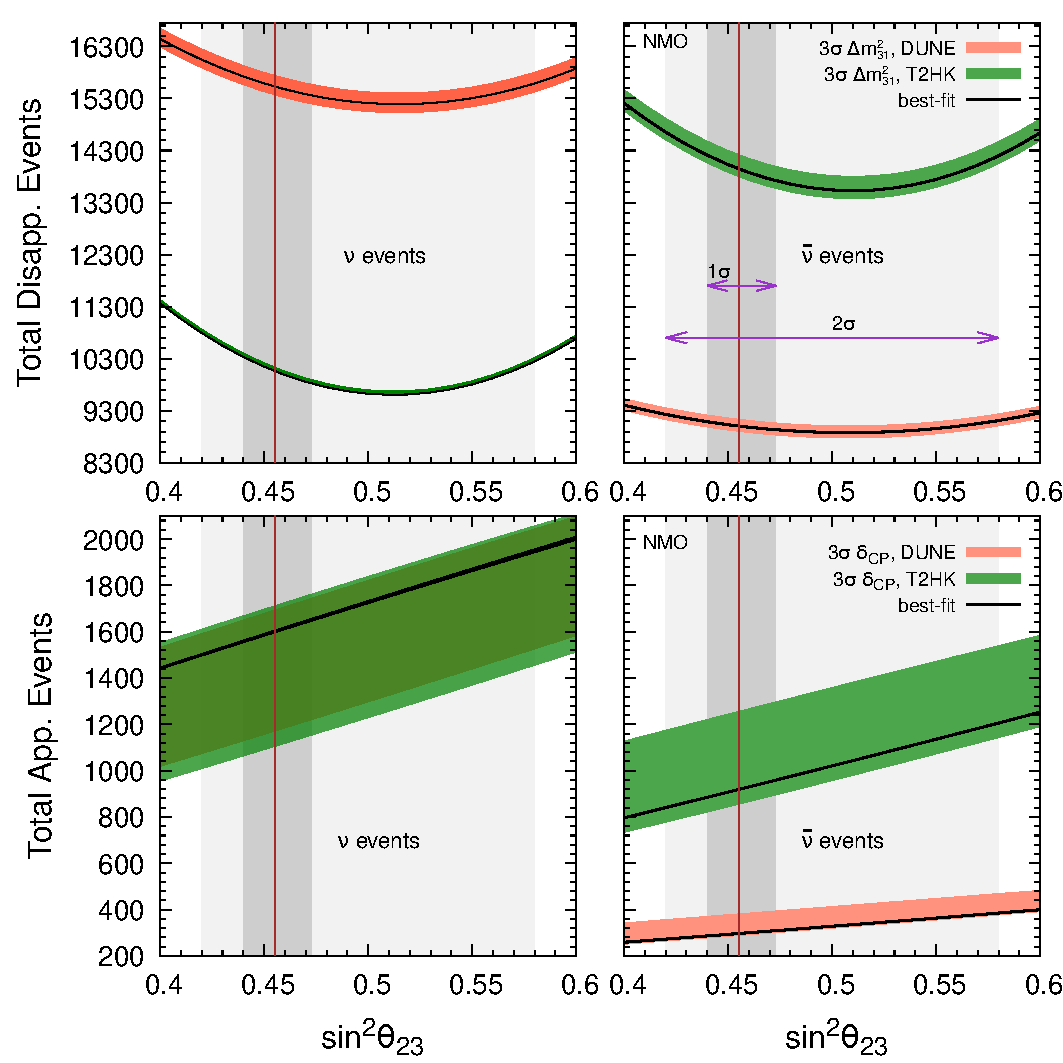
\includegraphics[width=\linewidth]{./Figures/Chapter-5/Test_events.pdf}
	\caption{\footnotesize{Total (only signal) disappearance and appearance event rates as a function of $\sin^2\theta_{23}$ in DUNE and T2HK assuming NMO. The left and right panel depicts the same in neutrino and antineutrino modes for 480 kt$\cdot$MW$\cdot$yr and 2431 kt$\cdot$MW$\cdot$yr of exposure in DUNE and T2HK, respectively. Band depicts $~3\sigma$ uncertainty in $\Delta m^2_{31}$ (upper panel) and $\delta_{\rm CP}$ (lower panel). 
 }}
	\label{fig:1}
\end{figure}
%----------------------------------------------------
In principle, reconstructing the charge of muons (to identify and segregate neutrinos from antineutrinos), event-by-event, is not feasible in DUNE and T2HK. There is always the occurrence of ``wrong-sign'' $ \bar{\nu}_{\mu}\, (\nu_{\mu})$ charged-current (CC) events when the primary beam is $\nu_{\mu} (\bar{\nu}_{\mu})$. Similarly, there is the contamination of ``wrong-sign'' $ \bar{\nu}_{e}\, (\nu_{e})$ charged-current (CC) events in neutrino (antineutrino) modes. \\
For the energy range under consideration, there is suppression in both the antineutrino cross-section and flux than a neutrino, which leads to a relatively more contribution of wrong-sign $\nu_{\mu}$ CC events in antineutrino mode than its counterpart. Apart from this, in Nature, positive mesons are more abundant than their negative counterpart as they are produced following the $pp$ or the $pn$ collisions~\cite{Dore:2018ldz}. Therefore, the neutrino beam is more intense than the antineutrino beam, and hence, the contamination of wrong-sign neutrinos in the antineutrino beam is higher. Both DUNE and T2HK follow horn current terminology, where the neutrino-enhanced beam is coined as forward horn current (FHC), and the antineutrino-enriched beam is the reverse horn current (RHC). In FHC, the wrong-sign flux is concentrated in the high-energy tail of the flux spectrum, where leptons are more likely to be forward and energetic due to the kinematics of neutrino and antineutrino scattering, while in RHC, they are concentrated around the low reconstructed energies~\cite{Katori:2016yel, DUNE:2020jqi}. Therefore, in general, we expect that the number of $\bar{\nu}$ events in $\nu$ beam to be way lesser than contamination of ${\nu}$ beam with $\bar{\nu}$. 
  

In table \ref{table:two}, we compute the total event rates (signal) in $\nu_\mu\rightarrow\nu_\mu$ disappearance channel and $\nu_\mu\rightarrow\nu_{e}$ appearance channel for both neutrino and antineutrino modes in DUNE and T2HK, using benchmark oscillation parameters (refer to table~\ref{table:one}) with and without the inclusion of wrong-sign events. From the illustrative events shown in table~\ref{table:two} under two scenarios, we observe that the contribution from wrong-sign events is more in the RHC ($\bar{\nu}$ mode) than in FHC ($\nu$ mode). Moreover, in RHC, this contamination is more for the disappearance event rates (~50\% in DUNE, 35\% in T2HK) than appearance rates (~36\% in DUNE and ~17\% in T2HK). Consequently, given its larger size, T2HK is likely to exhibit greater effects from this contamination than DUNE. Following the general convention, in all our analyses henceforth, we have considered the wrong-sign contributions in both FHC and RHC signal events for both DUNE and T2HK.


%---------------------------------------------------
\subsection{Total appearance and disappearance event rates}
\label{sec:2d}

Figure~\ref{fig:1} illustrates the total disappearance and appearance event rates in DUNE and T2HK. While the disappearance rates are affected mostly by uncertainty in $\Delta m^{2}_{31}$ and $\sin^{2}\theta_{23}$, the uncertainty in $\delta_{\rm CP}$ and $\sin^{2}\theta_{23}$ affects appearance rates predominantly, therefore we show bands of currently allowed 3$\sigma$ in $\Delta m^2_{31}$ for disappearance and $\delta_{\rm CP}$ in appearance event rates. The disappearance rates follow a U-shaped distribution when studied as a function of $\sin^{2}\theta_{23}$. This is because the disappearance rates $\propto (1-\sin^{2}\theta_{23})$. This points towards multiple combinations of $\sin^{2}\theta_{23}-\Delta m^2_{31}$ with same number of events~\cite{Agarwalla:2021bzs, Agarwalla:2022xdo}. Further, we observe that for values of $\sin^{2}\theta_{23}$ in the HO but close to 0.5, the curves show a flat behavior in both DUNE and T2HK. This hints that for these values of $\sin^{2}\theta_{23}$, sensitivity towards deviation from maximality will mostly come from the appearance rates, while disappearance rates may dominate later. Also, the minimum is not exactly at 0.5; instead, it is seen slightly shifted towards HO due to finite $\theta_{13}$ correction~\cite{Raut:2012dm}. Following higher runtime, more expected flux in neutrino mode, and substantial matter effect, we expect higher neutrino statistics in DUNE than T2HK, keeping NMO fixed. Similarly, higher runtime in antineutrino mode for T2HK implies higher antineutrino statistics. Having access to a wide-band beam makes DUNE capable of analyzing several $L/E$ ratios and more susceptible to a change in the value of $\Delta m^{2}_{31}$, unlike T2HK. This explains the higher neutrino disappearance statistics and a wider band when we vary $\Delta m^{2}_{31}$ in DUNE relative to T2HK. Further, DUNE's access to both the first and second oscillation maxima assures high disappearance rates in neutrino mode~\cite{DUNE:2020jqi} than T2HK, which has relatively fewer events at the second oscillation maximum~\cite{Hyper-Kamiokande:2018ofw}. In antineutrino mode, a higher runtime overcomes cross-section suppression in T2HK, which is not observed in the case of DUNE. Considering the appearance events in neutrino mode, DUNE has a higher runtime but lesser exposure, while T2HK has a lesser runtime but higher exposure; therefore, both experiments have almost similar event rates. In contrast, T2HK has higher statistics in $\bar{\nu}$ mode due to more runtime than DUNE.

Below, we show how the above contrasting features grant DUNE and T2HK the capability to probe atmospheric parameters organically, complementing each other.


%%%%%%%%%%%%%%%%%%%%%%%%%%%%%%%%%%%%%%%%%%%%%%%%%
\section{Projected sensitivities and its variation with total exposure}
\label{sec:results}
%%%%%%%%%%%%%%%%%%%%%%%%%%%%%%%%%%%%%%%%%%%%%%%%%%
We project the expected sensitivities in DUNE, T2HK, and their combination to study the atmospheric parameters based on the detailed computation of event rates discussed above. Our results and analyses are based upon the current scenario in 3$\nu$ paradigm from the global oscillation data answering three crucial questions: (i) establishing deviation from maximal $\theta_{23}$, (ii) precision measurements in the 2-3 sector; $\sin^2\theta_{23}$ and $\Delta m^2_{31}$\,, and (iii) rejecting the wrong octant solutions of $\sin^2\theta_{23}$. Following the definition of Poissonian $\chi^2$~\cite{Baker:1983tu}, we estimate the median sensitivity~\cite{Cowan:2010js} of a given experiment in the frequentist approach~\cite{Blennow:2013oma} as  
%
\begin{equation}
\chi^2 (\vec{\omega}, \, \kappa_{s}, \, \kappa_{b,l})= \underset{( \vec{\lambda}, \, \kappa_{s}, \,\kappa_{b,l})}{\mathrm{min}}\left\{  2\sum_{i=1}^{n}(\tilde{y_i}-x_i-x_i\mathrm{ln}\frac{\tilde{y_i}}{x_i})+\kappa^2_{s}+ \sum_{l}\kappa^2_{b,l}\right\}\, , 
\label{eq:chi2} 
\end{equation}
%
where $n$ is the total number of reconstructed energy bins and $\vec{\lambda}$ is the set of oscillation parameters that are marginalized in the fit. The choice of set $\vec{\lambda}$ is discussed later in every subsection. Further,
%
\begin{equation}
\tilde{y_i}\,(\vec{\omega},\{\kappa_{s},\kappa_{b,l}\}) = N^{th}_i(\vec{\omega})[1+\pi^s\kappa_{s}] + \sum_{l}N^b_{i,l}(\vec{\omega})[1+\pi^b\kappa_{b,l}]\, .
\label{chi}
\end{equation}
%
Here, $N^{th}_i\,(\vec{\omega})$ is the number of signal events predicted in the $i$-th energy bin for a given set of oscillation parameters $\vec{\omega} = \left\lbrace \theta_{23}\,,\theta_{13}\,,\theta_{12}\,,\Delta \mathrm{m}^{2}_{21}\,, \Delta \mathrm{m}^{2}_{31}\,,\delta_{\mathrm{CP}}\right\rbrace$. $N^{b}_{i,l}\,(\vec{\omega})$ denotes the number of background events in the $i$-th energy bin where the neutral current (NC) backgrounds are independent of the oscillation parameter $\vec{\omega}$, while the charged current (CC) backgrounds is dependent on the oscillation parameters. $\pi^s$ is the pull term for systematic uncertainty on signal events. $\pi_{b,l}$ is the pull term for the systematic uncertainties on the $l$-th background contribution for any given channel in signal. These pull terms are uncorrelated with one another and have the same values in neutrino and antineutrino modes.  We incorporate the corresponding data in Eq.~\ref{eq:chi2} using the variable $x_{i}= N^{ex}_i\, +\, N^b_{i,l}$, where $N^{ex}_i$ indicates the observed CC signal events in the $i$-th energy bin via $\nu_{\mu}\rightarrow \nu_{\mu}$ and $\bar{\nu}_{\mu}\rightarrow \bar{\nu}_{\mu}$ disappearance channels and $\nu_{\mu}\rightarrow \nu_{e}$ and $\bar{\nu}_{\mu}\rightarrow \bar{\nu}_{e}$ appearance channels. Here, $N^b_{i,l}$  represents the $l$-th background contribution for a given channel. Throughout the simulation, we use publicly available software GLoBES~\cite{Huber:2002mx, Fogli:2002pt, Gonzalez-Garcia:2004pka}. We fix the mass ordering to NMO while generating data, as there are weak hints from global oscillation data favoring NMO at $\sim 2.5\sigma$~\cite{Capozzi:2021fjo, NuFIT}. In the fit, we marginalize over the allowed regions in oscillation parameters as mentioned in table~\ref{table:one}. We do not include any correlations among them as by the time these future experiments start taking data, these correlations will likely weaken~\cite{Song:2020nfh}. We consider the benchmark choices for $\theta_{12}$ and $\theta_{13}$ fixed~\cite{Capozzi:2021fjo}, as we do not expect the precision (2.8\%) achieved by Daya Bay to improve in the coming years~\cite{DayaBay:2022orm}. Although the present-day uncertainty in $\theta_{12}$ is 4.5\% ~\cite{Capozzi:2021fjo}, we do not expect the sensitivity in our study to get affected by it. We also fix the mass ordering in the fit as in the next decade, DUNE is expected to determine the mass ordering within initial years of data.

%----------------------------------------------------
\subsection{Establishing deviation from maximal $\sin^{2}\theta_{23}$}
%---------------------------------------------------
%----------------------------------------------------
\begin{figure}[htb!]
	\centering
	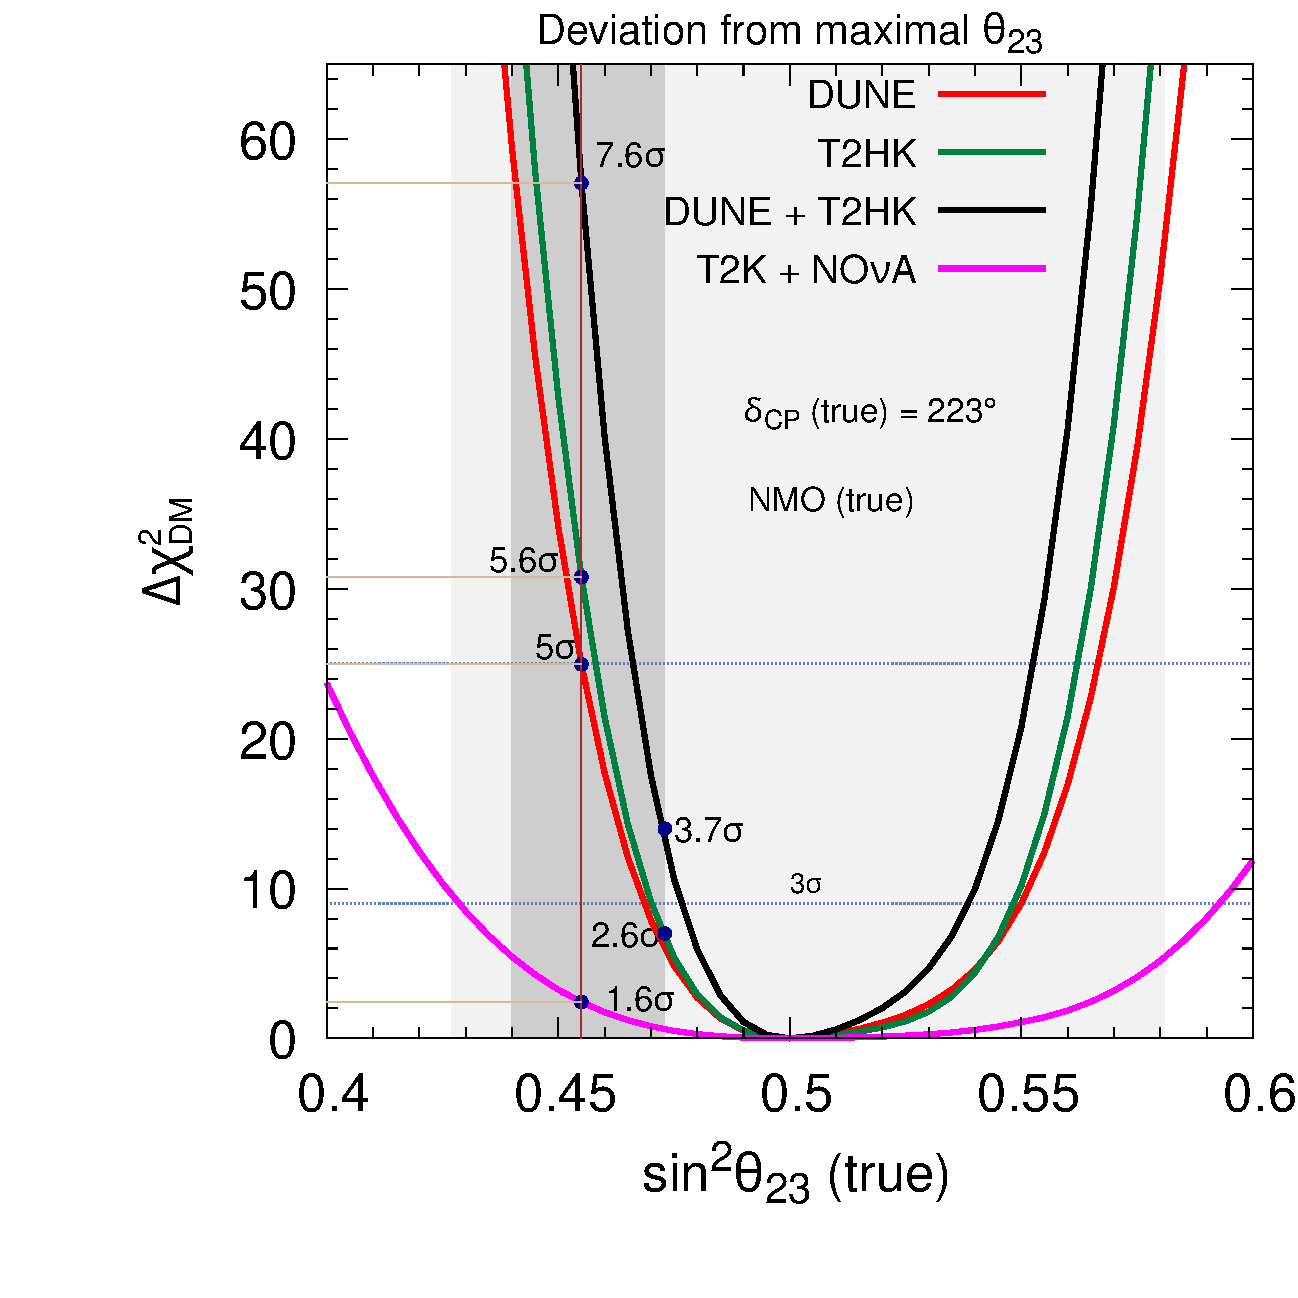
\includegraphics[width=0.8\linewidth]{./Figures/Chapter-5/v1_Three_experiments_octant_deviation_marg_223}
	\caption{\footnotesize{ Sensitivity of DUNE, T2HK, DUNE + T2HK, and T2K [2.5 yr ($\nu$) + 2.5 yr ($\bar{\nu}$)] + NO$\nu$A [3 yr ($\nu$) + 3 yr ($\bar{\nu}$)] to exclude non-maximal solutions of $\sin^{2}\theta_{23}$ as a function of $\sin^2\theta_{23}$ in the data. For benchmark choices of oscillation parameters and the allowed ranges in $\Delta m^{2}_{31} $ and $\delta_{\rm CP}$ over which we marginalize in the fit, refer to table~\ref{table:one}. We assume exposures of 480 kt$\cdot$MW$\cdot$yr in DUNE, 2431 kt$\cdot$MW$\cdot$yr in T2HK, $84.4$ kt$\cdot$MW$\cdot$yr in T2K, and 58.8 kt$\cdot$MW$\cdot$yr in NO$\nu$A. For illustrative purpose, the benchmark choices of $\sin^{2}\theta_{23}$ is shown by a vertical brown line, projecting out the statistical confidence at the intersection with each curve. \textit{If in Nature, $\sin^{2}\theta_{23}$ is around the lower value of current 1$\sigma$ uncertainty ($\sim 0.473$), then the combination is the only solution to achieve $3\sigma$ with current benchmark values.} 
 }} 
	\label{fig:DM}
\end{figure}
%----------------------------------------------------
We compute the statistical confidence with which DUNE, T2HK, and DUNE + T2HK can establish a deviation from maximal $\sin^{2}\theta_{23}$ by following 
\begin{equation}
\Delta \chi^2_{\text{DM}}= \underset{\delta_{\mathrm{CP}}\,,\,\Delta m^{2}_{31}}{\mathrm{min}}\left\{ \chi^2\left(\sin^2\theta_{23}^{\mathrm{test}} = 0.5\right)-\chi^2\left(\sin^2\theta_{23}^{\mathrm{true}} \in [0.4,0.6]\right) \right\},
\label{eq:deviation-from-maximality-chi2}
\end{equation}
where, $\vec{\lambda} = \{\delta_{\mathrm{CP}}, \, \Delta m^{2}_{31}\}$ is the set of oscillation parameters over which $\Delta\chi^2_{\rm DM}$ gets marginalized in the fit. So we generate the data for allowed uncertainty in $\sin^{2}\theta_{23}$ (refer to table~\ref{table:one}), while fixing it to 0.5 in the fit. There have been previous studies along this direction in ref.~\cite{Ballett:2016daj}\,, however here we consider the current best-fit values from ref.~\cite{Capozzi:2021fjo} which are similar to other global oscillation studies~\cite{NuFIT, Esteban:2020cvm, deSalas:2020pgw}. We also incorporate the latest collaboration estimates and ancillary files while using GLoBES.
%----------------------------------------------------
\begin{figure}[t!]
	\centering
	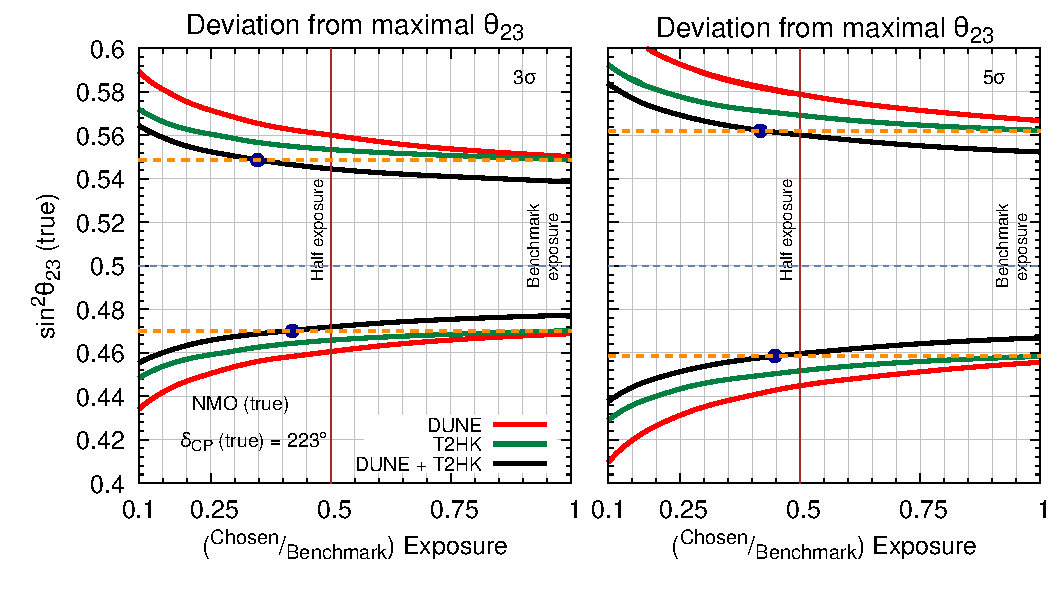
\includegraphics[width=\linewidth]{./Figures/Chapter-5/Final_DM_exposure}
	\caption{\footnotesize{3$\sigma$  (5$\sigma$) sensitivity of non-maximal $\sin^{2}\theta_{23}$ as a function of scaled (ratio of the chosen to the benchmark value of) exposure, assuming true NMO in the left (right) panel. The ratio reaches 1 at the benchmark choices of the corresponding experimental setups. We generate data by fixing all other oscillation parameters except $\sin^{2}\theta_{23}$ to their best-fit value (see table~\ref{table:one}). We marginalize over $\delta_{\mathrm{CP}}$ and $\Delta m^2_{31}$ in the test-statistics using the ranges of marginalization in table~\ref{table:one}. Dashed orange lines and solid blue circles are used to project and compare the maximum sensitivity attainable by standalone DUNE and T2HK using their nominal exposures with the exposure needed by DUNE + T2HK to achieve the same sensitivity. \textit{We find that using approximately 40\% of their exposures, DUNE + T2HK together achieves comparable sensitivity to each experiment independently running at their nominal exposures.}
  }}
	\label{fig:Exposure_DM}
\end{figure}
%--------------------------------------------------

Figure~\ref{fig:DM} depicts the sensitivity in establishing deviation from maximality ($\Delta \chi^2_{\rm DM}$ in Eq.~\ref{eq:deviation-from-maximality-chi2}) as a function of true $\sin^{2}\theta_{23}$ for DUNE, T2HK, and their combination. As expected, it is smallest when the true and test equals for $\sin^{2}\theta_{23}$, increasing on both sides as we go away, implying the major contribution from $\sin^{2}2\theta_{23}$ in the leading term of disappearance channel (refer to an elaborate discussion in ref.~\cite{Agarwalla:2021bzs}). However, the U-shape around the $\sin^{2}\theta_{23} = 0.5$ is not symmetric because of the non-zero value of $\theta_{13}$. We observe that even after using the projected full exposure in the present-day long-baseline experiments: T2K and NO$\nu$A; they have lesser sensitivities. One of the major drawbacks in the present-generation experiments is much higher systematic uncertainties in both $\nu_{\mu}\rightarrow \nu_{\mu}$ and $\bar{\nu}_{\mu}\rightarrow \bar{\nu}_{\mu}$ disappearance rates (refer to last paragraph in Sec.~\ref{sec:2a} for corresponding values). The spread of curve around $\sin^{2}\theta_{23} = 0.5$ in all the experimental setups is less when $\sin^{2}\theta_{23} < 0.5$ than $\sin^{2}\theta_{23} > 0.5$. This can be explained due to the finite $\theta_{13}$ corrections~\cite{deGouvea:2005hk, Coloma:2012ut, Raut:2012dm} (Also, refer to discussion around fig.~\ref{fig:1} in Sec.~\ref{sec:2d}). Establishing sensitivity to deviations from maximality primarily depends on the disappearance statistic. In ref.~\cite{Agarwalla:2021bzs}, we also analyze and infer that uncertainty in the values of $\delta_{\mathrm{CP}}$ have minimal impact on this sensitivity. While T2HK, owing to huge disappearance statistics and corresponding lesser expected systematic uncertainties (refer to Sec.~\ref{sec:2a}), is able to achieve better sensitivity than DUNE, DUNE provides better measurements of $\Delta m^{2}_{31}$. Their combination (DUNE + T2HK) makes use of the complementary features among them and achieves a nearly 8$\sigma$ statistical confidence in establishing non-maximal $\sin^{2}\theta_{23}$, considering full exposures in the two experiments and the benchmark values. Furthermore,  \textit{if in Nature, $\sin^{2}\theta_{23}$ is around the upper value of current 1$\sigma$ uncertainty ($\sim 0.473$), then the combination is the only solution to achieve $3\sigma$ with current benchmark values.}

 The product of runtime, fiducial detector mass, and beam power provides the expected experimental exposure. The quantity of exposure is often considered interchangeably with runtime in phenomenological studies of neutrino oscillation. Currently, the DUNE collaboration also envisions a staged approach instead of undertaking the mammoth task of setting up a full-fledged DUNE detector of 40 kt fiducial mass~\cite{DUNE:2020jqi}. Therefore, it becomes imperative to discuss sensitivity study as a function of exposure. In figure~\ref{fig:Exposure_DM}, we study the nature of $\Delta \chi^2_{\rm DM}$ at 3$\sigma$ and 5$\sigma$ in Eq.~\ref{eq:deviation-from-maximality-chi2} as a function of scaled exposure for the standalone DUNE, T2HK, and their combination. We observe that initially, with an increase in exposure, the sensitivity to establish the deviation from maximal $\theta_{23}$ increases. However, the sensitivity after reaching half of their individual benchmark exposures reaches almost saturation. Horizontal illustrative dashed orange lines are drawn to depict the values of true $\sin^2\theta_{23}$ beyond which T2HK cannot differentiate between MM and the true values of $\sin^{2}\theta_{23}$ at its standard exposure, while the blue dots represent the intersection of the dashed orange line with the projected sensitivity curve of DUNE + T2HK. This implies that given the current benchmark choices of oscillation parameters in table~\ref{table:one}\,, the range of true values of $\sin^{2}\theta_{23}$ that can be differentiated from MM choices, by DUNE + T2HK with just $\sim 0.5$ of their nominal exposures, cannot be achieved by either of the individual experiments even with their respective projected exposures. When statistics are less, systematics become crucial. Therefore, at lower exposure, T2HK always performs better than DUNE to establish non-maximal $\sin^{2}\theta_{23}$, irrespective of the lower or higher octant of true choices of $\sin^{2}\theta_{23}$, because of better systematic uncertainties in disappearance rates. However, with the increment in exposure, the disappearance statistics in both DUNE and T2HK become similar. The complementary between DUNE + T2HK is essential to achieve a significant sensitivity at 5$\sigma$, even with high exposure. While the high precision measurements of DUNE in $\Delta m^{2}_{31}$ (due to substantial matter effect), complements the sensitivity of DUNE + T2HK at lower exposure, figure~\ref{fig:Exposure_DM} clearly shows that after a certain exposure, this study is no longer statistics-driven for achieving the sensitivity at 3$\sigma$. Nevertheless, a higher confidence level (5$\sigma$) is predominantly statistics-driven.

 %----------------------------------------------------
%----------------------------------------------------
\subsection{Exclusion of wrong octant solutions of $\sin^{2}\theta_{23}$} 
%----------------------------------------------------
%----------------------------------------------------
\begin{figure}[htb!]
	\centering
	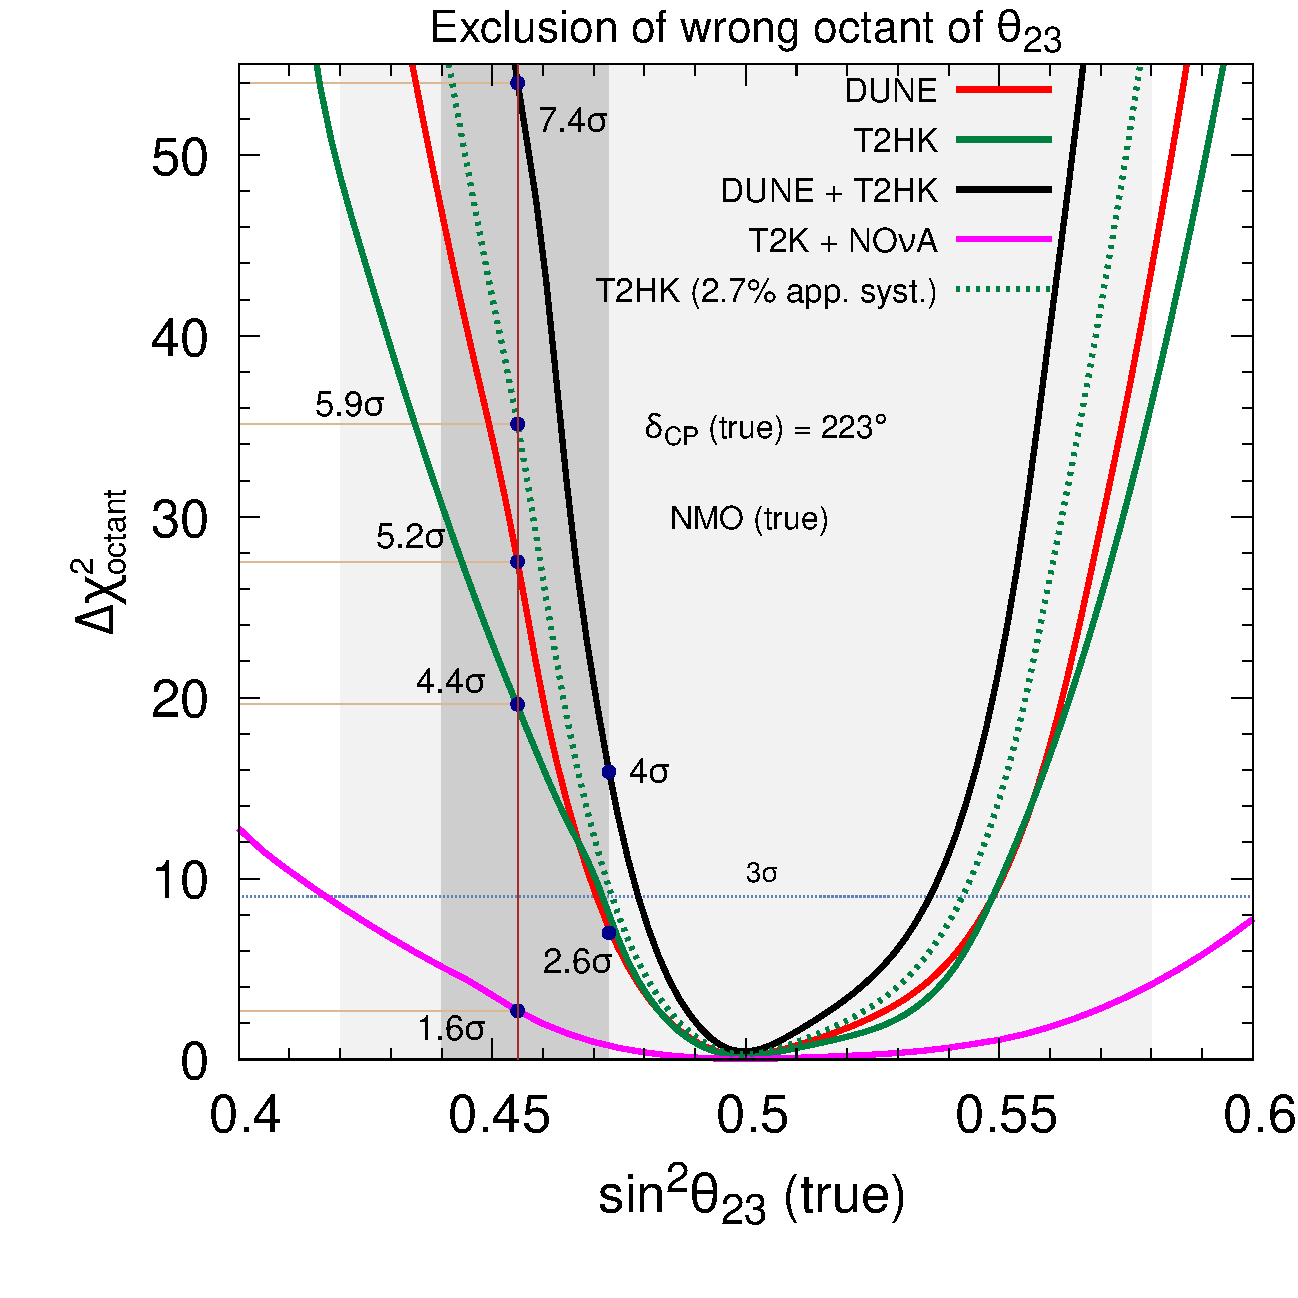
\includegraphics[width=0.8\linewidth]{./Figures/Chapter-5/Octant_exclusion_smooth}
	\caption{\footnotesize{ Sensitivity towards exclusion of wrong octant solutions in DUNE, T2HK, their combination, and T2K [2.5 yr $(\nu)$ + 2.5 yr $(\bar{\nu})$] + NO$\nu$A [3 yr $(\nu)$ + 3 yr $(\bar{\nu})$] as a function of $\sin^{2}\theta_{23}$ in data. The sensitivity of T2HK with an estimated improvement of nominal appearance systematic uncertainties to 2.7\% is also shown. In the fit, we marginalize over $\Delta m^{2}_{31}$ and $\delta_{\rm CP}$, keeping others fixed at their best-fit values (refer to table~\ref{table:one}). For illustrative purposes, we project out the statistical confidence for each curve, when $\sin^{2}\theta_{23} = 0.455$ in data.
 }}
	\label{fig:octant exclusion}
\end{figure}
%----------------------------------------------------
%--------------------------------------------------
\begin{figure}[htb!]
	\centering
	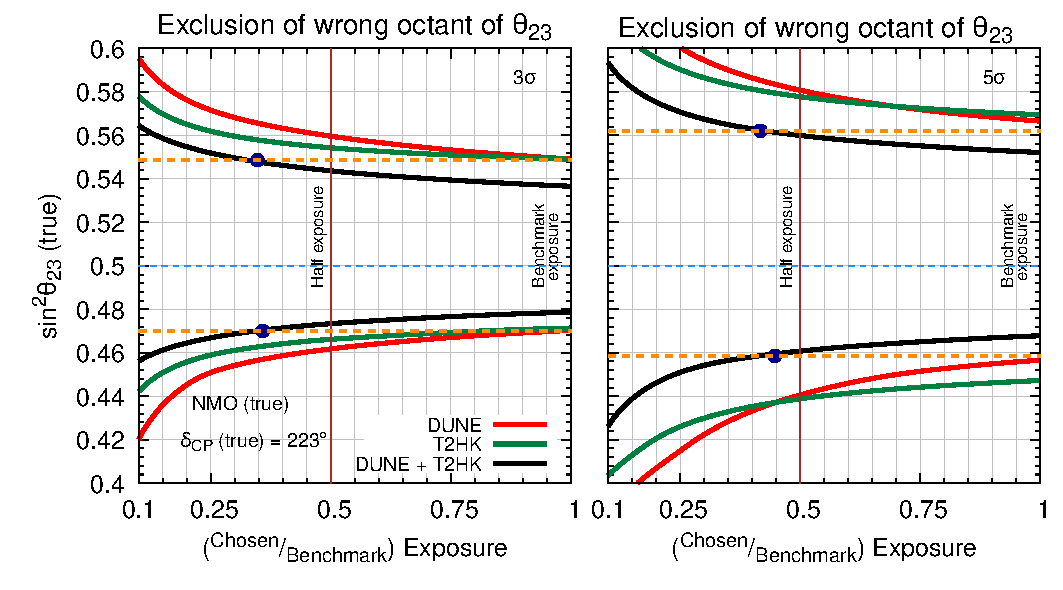
\includegraphics[width=\linewidth]{./Figures/Chapter-5/Final_Exposure_octant_exclusion}
	\caption{\footnotesize{3$\sigma$  (5$\sigma$) exclusion of wrong octant of $\sin^{2}\theta_{23}$ as a function of scaled exposure is shown in left (right) panel. 1 depicts the benchmark exposure. We marginalize over the allowed regions of $\delta_{\mathrm{CP}}$ and $\Delta m^2_{31}$ in the fit. Refer to table~\ref{table:one}. \textit{ At lower exposure, the complementarity between DUNE + T2HK is the only solution to attain a 5$\sigma$ discovery in ruling out the wrong octant solutions for a significant range of $\sin^2 \theta_{23}$ in Nature. 
 } }}
 \label{fig:octant-eclusion-vs-scaled-exposure}
 \end{figure}


%----------------------------------------------------
Following the discussion of deviation from maximality, we study in this section the efficiency in establishing the octant of $\sin^{2}\theta_{23}$ by rejecting the hypothesis of wrong octant solutions. For this, we define 
\begin{eqnarray}
    \Delta \chi^{2}_{\text{octant}} &=& \underset{(\vec{\lambda})}{\mathrm{min}}\left\{ \chi^2\left(\sin^2\theta_{23}^{\mathrm{test}} \right) - \chi^2\left(\sin^2\theta_{23}^{\mathrm{true}}\right)\right\}\,,
\label{eq:octant-exclusion-chi2}
\end{eqnarray}
where $\sin^{2}\theta_{23}^{\mathrm{true}}$ refers to one octant, say LO; then, we generate data with [0.4, 0.5), while in the fit, we use the opposite octant, which in this case is HO $\in (0.5,0.6]$. Similar changes can be made by generating data with HO and excluding the LO hypothesis in the theory. In Eq.~\ref{eq:octant-exclusion-chi2}\,, $\vec{\lambda} = \{ \Delta m^{2}_{31}, \delta_{\rm CP}\}$. We use the corresponding allowed ranges from table~\ref{table:one}. Figure~\ref{fig:octant exclusion} depicts $\Delta \chi^{2}_{\text{octant}}$ as a function of $\sin^{2}\theta_{23}$ with which we generate data. It shows that alone DUNE and T2HK have similar sensitivity. T2HK is more stringent at lower significance, and DUNE is stronger at higher confidence. Large appearance systematic uncertainties in T2HK do not deteriorate the sensitivity, at least for lower significance due to comparable neutrino and antineutrino statistics~\cite{Agarwalla:2021bzs}. However, for attaining a higher significance, better systematic uncertainties in appearance rates are essential, which is a characteristic feature in DUNE (refer to section~\ref{sec:events}). The complementarity between DUNE and T2HK improves the standalone experiments' performance by almost $\sim 1.5$ times for the benchmark values from table~\ref{table:one}. The effect of improved appearance systematic uncertainties is distinctly visible when we consider the expected 2.7\% in T2HK~\cite{Munteanu:2022zla} instead of the nominal 5\%. Once the systematics are improved, T2HK performs better than DUNE irrespective of the true values of $\sin^{2}\theta_{23}$ in Nature. Sensitivity towards the exclusion of the wrong octant is dependent on both disappearance and appearance statistics, with the latter being dominant. For consistency, we have also checked the octant exclusion sensitivity using the best fit values and their corresponding allowed 3$\sigma$ ranges for minimization in the test-statistics from ref.~\cite{NuFIT:current}. We find that the results align closely with those shown in figure~\ref{fig:octant exclusion}.

In figure~\ref{fig:octant-eclusion-vs-scaled-exposure}\,, we study the efficacy of experiments in isolation and combination in ruling out the wrong octant of $\sin^{2}\theta_{23}$ as a function of scaled exposure. We observe that with 0.25 of their nominal exposures, DUNE alone will be able to differentiate about $\sim 45\%$ of $\sin^{2}\theta_{23}$ from wrong octant solutions; this improves to $\sim 50\%$ in T2HK, while their combination, DUNE + T2HK can differentiate $\sim 60\%$. So with just 0.25 of their individual exposures, it is possible in the combined setup to exclude the wrong octant for more than half of currently allowed $\sin^{2}\theta_{23}$ (refer to table~\ref{table:one}) at 3$\sigma$. Increasing beyond half of the nominal exposure does not help much, as the exclusion of the wrong octant solutions no longer remains statistics-driven. Further improvement in the allowed ranges of $\delta_{\mathrm{CP}}$ from the ongoing long-baseline experiments: T2K~\cite{T2K:2023smv} and NO$\nu$A~\cite{Carceller:2023kdz} may help to remove $(\sin^{2}\theta_{23} - \delta_{\mathrm{CP}})$ degeneracy and thus improve the sensitivity in wrong octant exclusion. We also notice that at 3$\sigma$ about $\sim 73\%$ of $\sin^{2}\theta_{23} \in [0.4, 0.6]$ can differentiate between correct and wrong octant solutions using the combined DUNE + T2HK setup, given the current benchmark values and projected exposure holds. For a higher confidence level (5$\sigma$), DUNE + T2HK is the only solution to attain sensitivity towards the exclusion of wrong octant solutions. We also observe that the discovery potential of DUNE + T2HK in excluding wrong octant solutions of $\sin^{2}\theta_{23}$, achievable with just $\sim$0.45 times of their individual exposures, is comparable to the sensitivity attained by standalone experiments using their nominal exposures.

%--------------------------------------------------


\subsection{Precision measurements of $\sin^{2}\theta_{23}$ and $\Delta m^{2}_{31}$}
\label{precisionapp}

\begin{figure}[htb!]
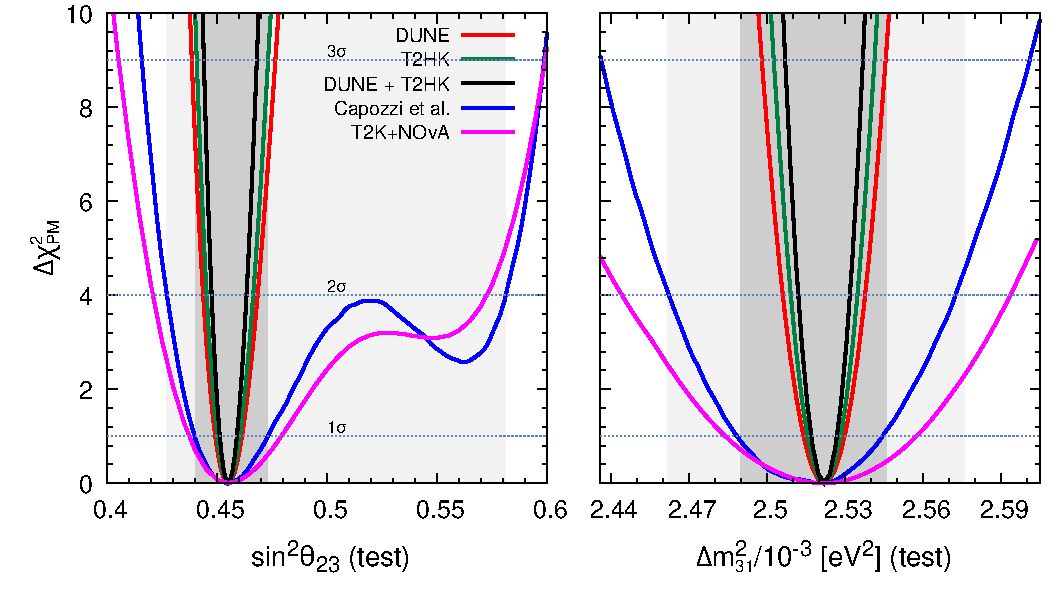
\includegraphics[width=\linewidth]{./Figures/Chapter-5/Test_precision}
\caption{\footnotesize{Expected achievable precision on $\sin^2\theta_{23}$ and $\Delta m^2_{31}$ around the respective benchmark values (refer to table~\ref{table:one}) using DUNE, T2HK, DUNE + T2HK, T2K [2.5 yr ($\nu$) + 2.5 yr ($\bar{\nu}$)] + NO$\nu$A [3 yr ($\nu$) + 3 yr ($\bar{\nu}$)], and global-fit from ref.~\cite{Capozzi:2021fjo}. In the fit, we marginalize over allowed region in $\delta_{\rm CP}$ and $\Delta m^{2}_{31}$ while determining precision on $\sin^2\theta_{23}$. Similarly, we perform marginalization over $\delta_{\rm CP}$ and $\sin^2\theta_{23}$ while determining precision measurements in $\Delta m^{2}_{31}$. Refer to table~\ref{table:four} for the computed values of the relative 1$\sigma$ precision, following Eq.~\ref{precision1}.  
}}
\label{fig:6}
\end{figure}
%-------------------------------------------------------
%---------------------------------------------------------
\begin{table}[t!]
	\centering
	\resizebox{\columnwidth}{!}{%
		\begin{tabular}{|c|c|c|c|c|c|c|}
			\hline
			\multirow{3}{*}{Parameter} & \multicolumn{6}{c|}{Relative 1$\sigma$ precision (\%)}\\
			\cline{2-7}
			& T2HK& DUNE & T2HK+DUNE & T2K+NO$\nu$A &Capozzi $et~al.$  & JUNO \\
			\hline
			$\sin^{2}\theta_{23}$ & 1.18 & 1.40 & 0.88 & 7.10 & 6.72 & ---\\
			\hline
			$\Delta m^{2}_{31}$ & 0.25& 0.31 & 0.20 & 0.99 & 1.09 & 0.2\\
			\hline
		\end{tabular}
	}
\caption{\footnotesize{Relative 1$\sigma$ precision computed from figure~\ref{fig:6}, following Eq.~\ref{precision1}. In addition, we also give present-day global-fit precision from ref.~\cite{Capozzi:2021fjo} and expected relative 1$\sigma$ precision using JUNO with an estimated 6 years of run~\cite{NavasNicolas:2023fza}. }}
\label{table:four}
\end{table}
%-----------------------------------------------------------
\begin{figure}[t!]
	\centering
	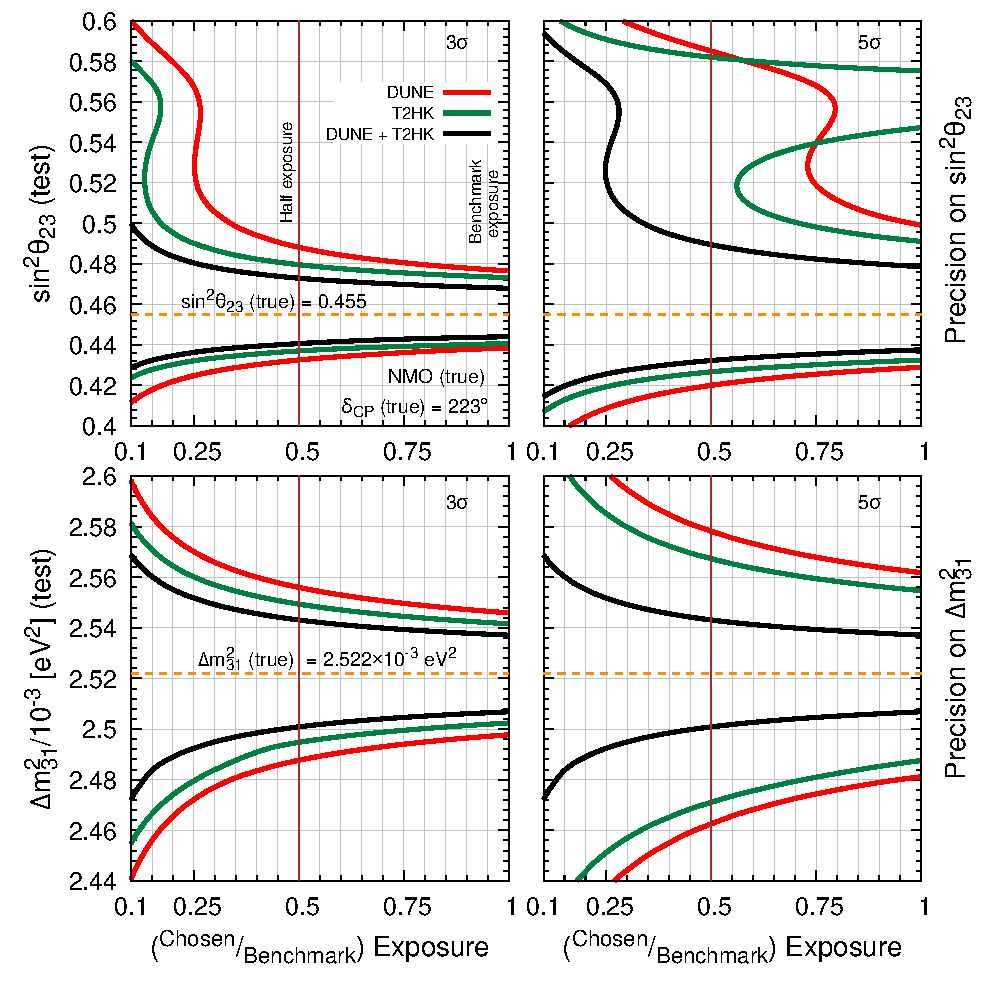
\includegraphics[width=\linewidth]{./Figures/Chapter-5/Test_precision_exposure}
	\caption{\footnotesize{Precision on $\sin^2\theta_{23}$ and $\Delta m^2_{31}$ around their benchmark values (refer to table~\ref{table:one}) as a function of scaled exposure is shown. The upper (lower) panel depicts the precision on $\sin^2\theta_{23}$ ($\Delta m^2_{31}$) at two different C.L. In the fit, we marginalize over the allowed ranges in  $\delta_{\mathrm{CP}}$ and $\Delta m^2_{31}$ ($\sin^2\theta_{23}$) while producing upper (lower) panel. \textit{Considering the benchmark choices, high statistical confidence (5$\sigma$) precision on both $\sin^2\theta_{23}$ and $\Delta m^2_{31}$ that can be achieved by DUNE + T2HK with just 0.25 of their individual exposures cannot be attained by standalone experiments even with their full exposures.} }}
	\label{figure:Exposure_precision}
\end{figure}
%-----------------------------------------------------------
Following the exclusion of wrong octant solutions, it is imperative to question the precision in determining the value of atmospheric parameters: $\sin^2\theta_{23}$ and $\Delta m^2_{31}$. We compute the  statistical confidence for determining precision measurements on $\sin^{2}\theta_{23}$ by defining
\begin{equation}
\Delta \chi^2_{\text{PM}} = \underset{(\vec{\lambda})}{\mathrm{min}}\left\{ \chi^2\left(\sin^{2}\theta_{23}^{\mathrm{test}}\in [0.4,0.6] \right) - \chi^2\left(\sin^{2}\theta_{23}^{\mathrm{true}} = 0.455 \right)\right\}\,,
\label{precision-chisq-th23}
\end{equation}
while precision on $\Delta m_{31}^{2}$ is evaluated using
\begin{equation}
\Delta \chi^2_{\text{PM}} = \underset{(\vec{\lambda})}{\mathrm{min}}\left\{ \chi^2\left(\Delta m_{31}^{2,\mathrm{test}} \in [2.436,2.605]\times 10^{-3} \right) - \chi^2\left(\Delta m_{31}^{2,\mathrm{true}} = 2.522 \times 10^{-3} \right)\right\}\;.
\label{precision-chisq-m31}
\end{equation} 
 Here, test choices represent the corresponding allowed ranges of values, while the true choice is kept fixed at the benchmark choices (refer to table~\ref{table:one}). $\vec{\lambda}$ defines the set of oscillation parameters over which we perform marginalization in the fit given by $\vec{\lambda} = \{ \delta_{\rm CP}, \Delta m^{2}_{31}\}$ in Eq.~\ref{precision-chisq-th23} and $\vec{\lambda} = \{\delta_{\rm CP}, \sin^{2}\theta_{23}\}$ in Eq.~\ref{precision-chisq-m31}, respectively. For ease of quantifying, table~\ref{table:four} computes relative $1\sigma$-precision, defined as,
\begin{equation}
p(\zeta)\, =\, \frac{\zeta^{\rm max} - \zeta^{\rm min}}{6.0 \,\times \, \zeta^{\rm true}}\, \times \, 100\%\, .
\label{precision1}
\end{equation} 
Here, $\zeta^{\rm max}$ and $\zeta^{\rm min}$ depict the allowed upper and lower test values of each curve in the corresponding parameters (refer to figure~\ref{fig:6}) at $3\sigma$, respectively. We also quote the expected relative $1\sigma$-precision on $\Delta m^{2}_{31}$ from the upcoming reactor experiment, JUNO~\cite{NavasNicolas:2023fza} with the projected 6 years of runtime.

From figure~\ref{fig:6}\,, we observe that precision measurements in $\sin^2\theta_{23}$ allow a weak ($\sim 1.2\sigma$) clone solution in higher octant with the present global fit of oscillation data~\cite{Capozzi:2021fjo}. Although, with the full exposures of T2K + NO$\nu$A, we expect subtle improvement in it. However, the precision around the benchmark value of $\sin^2\theta_{23}$ is better using the present global fit oscillation data than the full projected exposures of present long-baseline experiments. This is because of huge disappearance statistics from other ongoing atmospheric experiments like Super-K and IceCube DeepCore. Similarly, we observe that the precision on $\Delta m^{2}_{31}$ using the global fit of oscillation data has already surpassed the expected precision using the full projected exposure of T2K + NO$\nu$A. This is mostly because of the input from reactor experiments like Daya Bay in the global fit. Additionally, we observe that due to the high energy resolution and large statistics in DUNE and T2HK, respectively, the standalone experiments can rule out the clone solution in $\sin^2\theta_{23}$. Comparatively, T2HK outperforms DUNE in precision measurements because of its extensive disappearance statistics and superior disappearance systematic uncertainties. A longer runtime in antineutrino mode also benefits T2HK, as both neutrino and antineutrino modes are crucial for achieving better precision measurements~\cite{Agarwalla:2013ju}. Table~\ref{table:four} helps in quantifying this improvement, showing the benefit of the interplay between DUNE and T2HK. Combining them improves the present-day~\cite{Capozzi:2021fjo} achievable precision on $\sin^2\theta_{23}$ and $\Delta m^2_{31}$ by a factor of $\sim$7 and $\sim$5, respectively. Further, we also make a comparison with the upcoming reactor experiment, JUNO~\cite{NavasNicolas:2023fza}. The achievable precision on $\sin^{2}\theta_{23}$ due to these next-generation experiments is truly remarkable.\\
In figure~\ref{figure:Exposure_precision}\,, we study precision on both the atmospheric parameters as a function of scaled exposure. While the appearance channel is dominated by $\sin^{2}\theta_{23}$, disappearance channel is mostly influenced by $\sin^{2}2\theta_{23}$~\cite{Mikheyev:1985zog,Wolfenstein:1977ue,Cervera:2000kp,Freund:2001ui}. Hence, in resolving the issue of the wrong octant, appearance events play a crucial role, while for achieving better precision around the correct octant, disappearance events are essential. While standalone DUNE and T2HK bearing low exposures ($\sim 0.25$ times nominal exposure) cannot rule out clone solutions in $\sin^{2}\theta_{23}$ at 3$\sigma$, the combined DUNE + T2HK provide degeneracy-free measurements. Furthermore for achieving a discovery potential (5$\sigma$), standalone DUNE is unable to rule out the clone solutions in $\sin^{2}\theta_{23}$ even after achieving the projected exposure, T2HK needs $\sim 0.8$ of nominal exposure for excluding the wrong octant solutions. However, \textit{DUNE + T2HK can provide degeneracy-free precision on $\sin^{2}\theta_{23}$ at 5$\sigma$ by considering only $\sim 0.3$ times of their individual benchmark exposures}. In the standalone setup, DUNE performs better than T2HK because of the higher systematic uncertainties assumed in the appearance events of T2HK (5\% refer section~\ref{sec:2a}) than DUNE (2\%). As discussed earlier, appearance events are responsible for fixing the correct octant of $\sin^2\theta_{23}$ and thus removing any clone solutions. The combined precision displays the benefit of synergy between DUNE and T2HK, which can accomplish 5$\sigma$ precision around the correct octant. Furthermore, we observe that reaching 3$\sigma$ precision becomes saturated after a while; thus, it is no longer statistics-dominated. However, a degeneracy-free precision can be achieved by DUNE + T2HK at 5$\sigma$ even at lesser exposures if $\sin^{2}\theta_{23}$ turns out to be in LO in Nature. Similarly, in the case of $\Delta m^{2}_{31}$, \textit{using approximately 20\% of the individual exposures of DUNE and T2HK together can achieve an impressive relative 1$\sigma$ precision of 0.25\%. However, at the same exposure level, standalone DUNE and T2HK cannot distinguish between the benchmark values of $\Delta m^{2}_{31}$ and the currently allowed ranges from Table~\ref{table:one} when analyzed at 5$\sigma$.}

%----------------------------------------------------------
\section{Allowed regions in ($\sin^{2}\theta_{23}- \delta_{\mathrm{CP}}$) plane}
\label{sec:contour}
\begin{figure}[htb!]
	\centering
	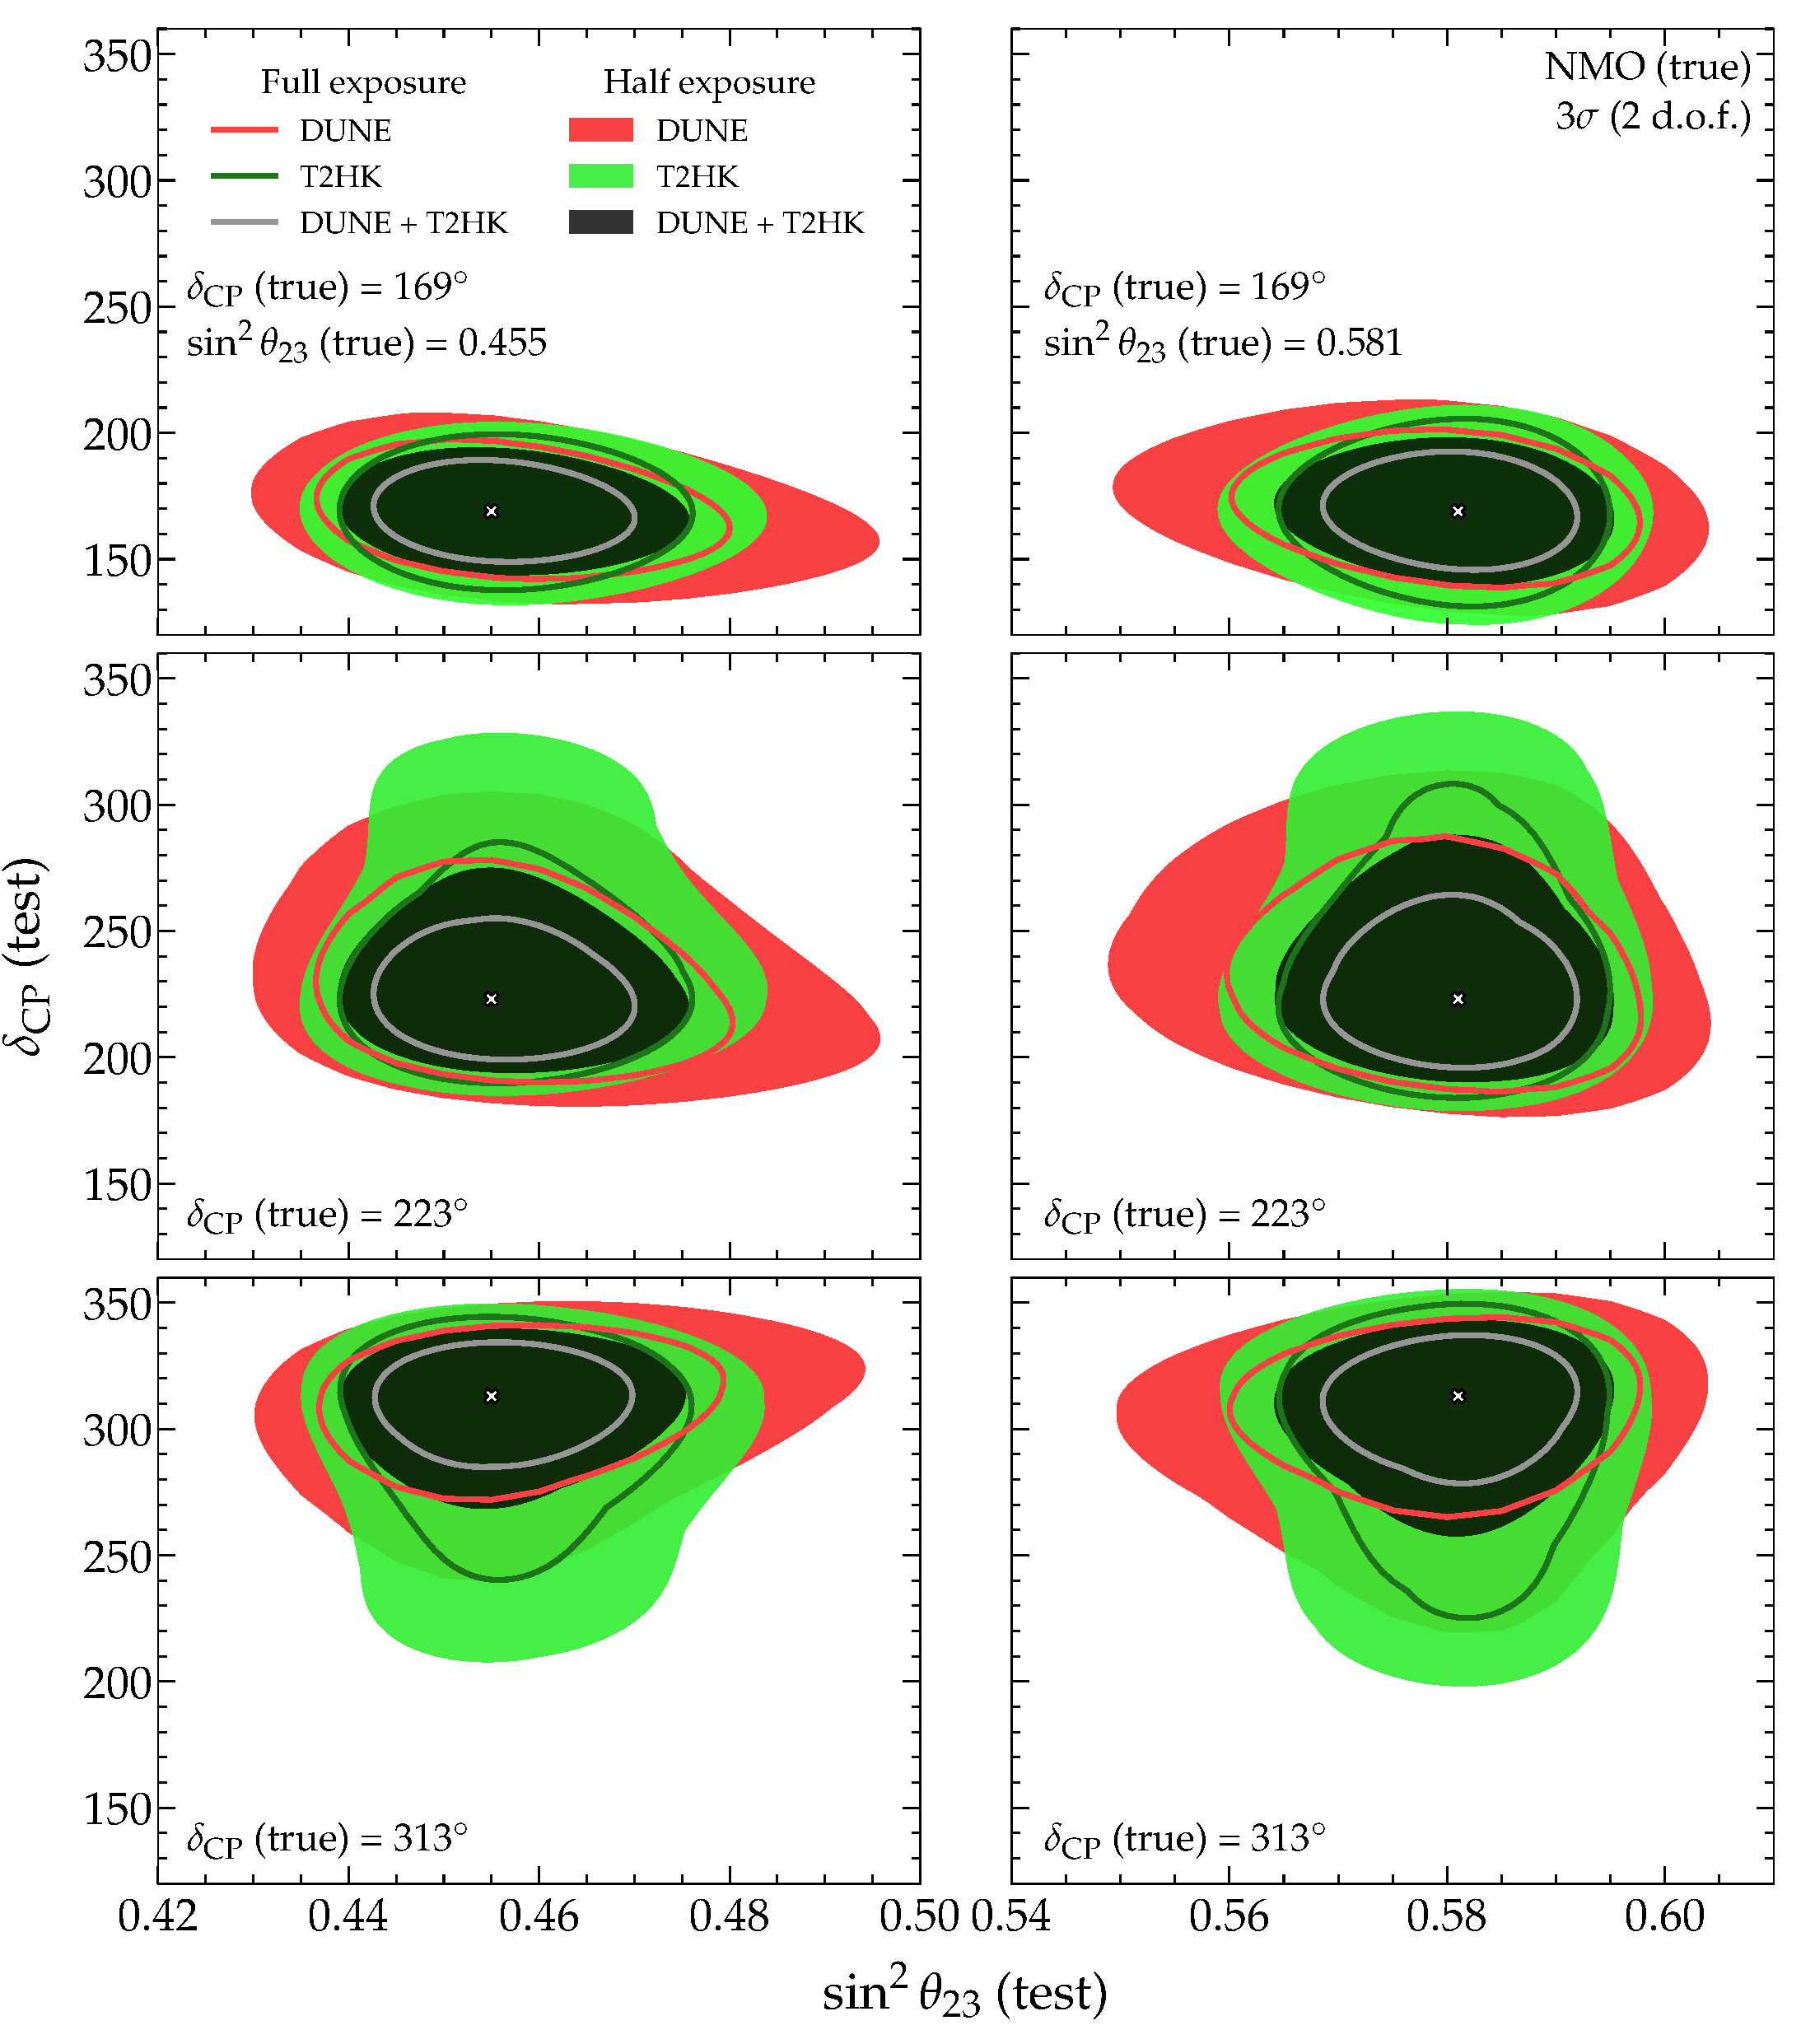
\includegraphics[width=\linewidth]{./Figures/Chapter-5/deltacp-theta23-combined}
	\caption{\footnotesize{Allowed regions of the test atmospheric mixing angle, $\sin^2\theta_{23}$  and CP phase, $\delta_\mathrm{CP}$. The true values correspond to the benchmark values and other illustrative choices following ref.~\cite{Capozzi:2021fjo} (see section~\ref{sec:contour} for detail). The test-statistics is scanned over $\sin^{2}\theta_{23}$  and $\delta_{\mathrm{CP}}$ (refer to Eq.~\ref{eq:chi-allowed-ranges}). \textit{Combination is the only solution to exclude clone solutions hinted by the standalone experiments at half exposures.}
 }}
	\label{fig:th23-dcp-allowed-ranges}
\end{figure}
%---------------------------------------------------------------
As discussed previously, appearance events are necessary for extracting the correct octant of $\sin^2\theta_{23}$, while disappearance events are essential in obtaining a high-precision around the correct octant of $\sin^2\theta_{23}$. In this section therefore, we study the correlation between $\sin^{2}\theta_{23}$ and $ \delta_{\mathrm{CP}}$ in light of the current allowed oscillation parameter space. For this, we follow
\begin{eqnarray}
    \Delta \chi^{2} &=& \underset{(\vec{\lambda},\, \Delta m^{2}_{31})}{\mathrm{min}}\left\{ \chi^2\left(\sin^{2}\theta_{23}^{\mathrm{test}}\in [0.4,0.6], \delta_{\mathrm{CP}}^{\mathrm{test}} \in [0^{\circ}, 360^{\circ}] \right) - \chi^2 (\sin^{2}\theta_{23}^{\mathrm{true}},\delta_{\mathrm{CP}}^{\mathrm{true}} )\right\},
    \label{eq:chi-allowed-ranges}
\end{eqnarray}
where we use the benchmark values, $\pm 2\sigma \text{ in } \delta_{\mathrm{CP}} = 169^{\circ}$ and 313$^{\circ}$, and + 2$\sigma$ in $\sin^{2}\theta_{23} = 0.581$, following ref.~\cite{Capozzi:2021fjo} to generate data in each panel while scanning over the mentioned ranges in Eq.~\ref{eq:chi-allowed-ranges} of $\sin^2\theta_{23}$ and $\delta_{\mathrm{CP}}$. We marginalize over allowed ranges in $\Delta m^{2}_{31}$ (refer table~\ref{table:one}) in the fit.

In figure~\ref{fig:th23-dcp-allowed-ranges}\,, the benefit of exploiting the complementarity between DUNE and T2HK is clearly visible. DUNE with wide-beam is able to analyze various $L/E$ ratios. It also has access to the second oscillation maximum and 2\% appearance systematic uncertainties due to the magnificent LArTPC detector. These attribute to a better precision around the CP phase. Moreover, the large matter effect due to the long baseline helps in better precision measurement of $\Delta m^{2}_{31}$. However, more matter effect also induces extrinsic CP, which deteriorates the precision measurements in CP phase. This can be resolved by T2HK; with less matter effect, it provides better access to the intrinsic CP phase. Further, the huge disappearance statistics help in obtaining a better precision on $\sin^{2}\theta_{23}$. For comparison, the efficacy of DUNE + T2HK is visible in excluding the clone solutions hinted by the standalone experiments (in middle and lower panels), even with just half exposure. Further increasing the exposure from half to full in DUNE + T2HK leads to a quantitative decrement in the allowed region. For the upper panel, we observe that the allowed region is more or less similar in DUNE, T2HK, and the combination for the CP phase but varies with exposure for $\sin^{2}\theta_{23}$. This is because both DUNE and T2HK have better precision on $\delta_{\mathrm{CP}}$ when it is away from the CP-violating phases~\cite{Coloma:2012wq,Nath:2015kjg,Machado:2015vwa}. However, for achieving better precision on $\sin^{2}\theta_{23}$, large disappearance statistics are needed (therefore, T2HK consistently performs better than DUNE in this respect). Hence, a significant difference is visible when half exposure is increased to full exposure in the case of DUNE. However, the combination of both experiments is already performing well with their half exposures combined. While in the middle panel, we observe that the standalone experiments are hinting toward clone solutions --- T2HK in $\delta_{\mathrm{CP}}$ and DUNE in $\sin^{2}\theta_{23}$, the combination is able to precisely measure around the true values. The case in the lower panel is similar. Therefore, with half the exposures in each experiment, the combination is the only solution for better precision around the illustrative true values considered.\\
\section{Allowed regions in ($\sin^{2}\theta_{23}-\Delta m_{31}^{2}$) plane}
\label{appendix1}
\begin{figure}[htb!]
	\centering
	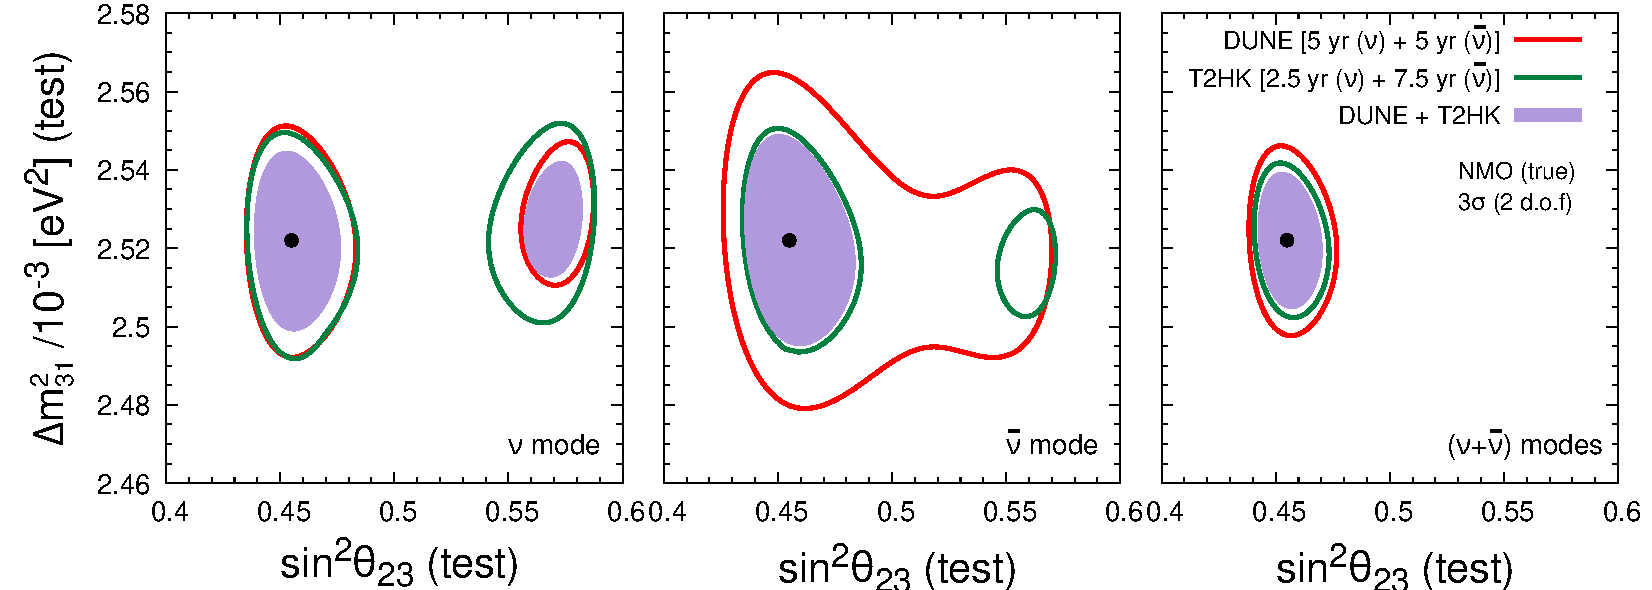
\includegraphics[width=\linewidth]{Figures/Chapter-5/New_Final_LO7_without_and_with_wsign.pdf}
	\caption{\footnotesize{Allowed regions of the test atmospheric mixing angle, $\sin^2\theta_{23}$  and mass-squared splitting, $\Delta m^2_{31}$. The true values correspond to the benchmark values as mentioned in table~\ref{table:one}. The test-statistics is scanned over $\sin^{2}\theta_{23}$  and $\Delta m^2_{31}$ (refer Eq.~\ref{eq:chi-allowed-ranges-th23-Dm31}). We marginalize over the allowed ranges in $\sin^{2}\theta_{23}$ in the fit. \textit{In only antineutrino mode, DUNE + T2HK is the only solution to exclude the clone solutions in $\sin^2\theta_{23}$.}
}}
        \label{fig:allowed-ranges-nmo}
\end{figure}
%---------------------------------------------------------------

We follow
%-------------------
\begin{eqnarray}
    \Delta \chi^{2} &=& \underset{(\vec{\lambda},\, \sin^{2}\theta_{23})}{\mathrm{min}}\left\{ \chi^2\left(\sin^{2}\theta_{23}^{\mathrm{test}}, \Delta m_{31}^{2 ~ \mathrm{test}} \right) - \chi^2 (\sin^{2}\theta_{23}^{\mathrm{true}},\Delta m_{31}^{2 ~ \mathrm{true}} )\right\}\,,
    \label{eq:chi-allowed-ranges-th23-Dm31}
\end{eqnarray}
%-------------------
for generating figure~\ref{fig:allowed-ranges-nmo}, where true values correspond to the benchmark values as mentioned in table~\ref{table:one}, while scanning over the test-statistics for $\sin^{2}\theta_{23}\in [0.4,0.6]$ and allowed ranges of $\Delta m^{2}_{31}$ in table~\ref{table:one}. Further, we also perform marginalization over allowed ranges of $\sin^{2}\theta_{23}$ in the fit. We perform this study, separately for neutrino, antineutrino, and combined modes. 

As discussed previously with respect to DUNE~\cite{DUNE:2020jqi} and many other references in literature~\cite{Agarwalla:2013ju}\,, both neutrino and antineutrino modes are essential for breaking the $\sin^{2}\theta_{23} - \delta_{\mathrm{CP}}$ degeneracy and ruling out the wrong octant solutions in standalone experiments, while running in only antineutrino mode performs differently for the combined DUNE + T2HK. Alone, DUNE, when run in only antineutrino mode, is unable to expel even the MM solution of $\sin^{2}\theta_{23}$, T2HK has a clone solution at higher octant apart from the true octant. However, the complementary features in the combination are sufficient for breaking the $\sin^{2}\theta_{23} - \delta_{\mathrm{CP}}$ degeneracy in only antineutrino mode, which was not possible in standalone experiments. This is because, in the combined scenario, while T2HK has higher $\bar{\nu}$ statistics (refer to section~\ref{sec:2a}) leading to a majority of appearance events free of contamination from matter-induced CP phase, DUNE provides better precision measurement in $\Delta m^{2}_{31}$. The third panel shows the same curves as depicted in figure~\ref{fig:moneyplot} with full exposures. Isolated DUNE and T2HK are already able to achieve good precision around the best-fit breaking the $\sin^{2}\theta_{23} - \delta_{\mathrm{CP}}$ degeneracy, which gets more stringent around the best-fit with the combination.

%==========================================================================
\section{Sensitivity in ($\sin^{2}\theta_{23}-\Delta m_{31}^{2}$) plane with near-future experiments}
\label{appendix2}
%==========================================================================

%---------------------------------------------------------------
\begin{figure}[htb!]
	\centering
	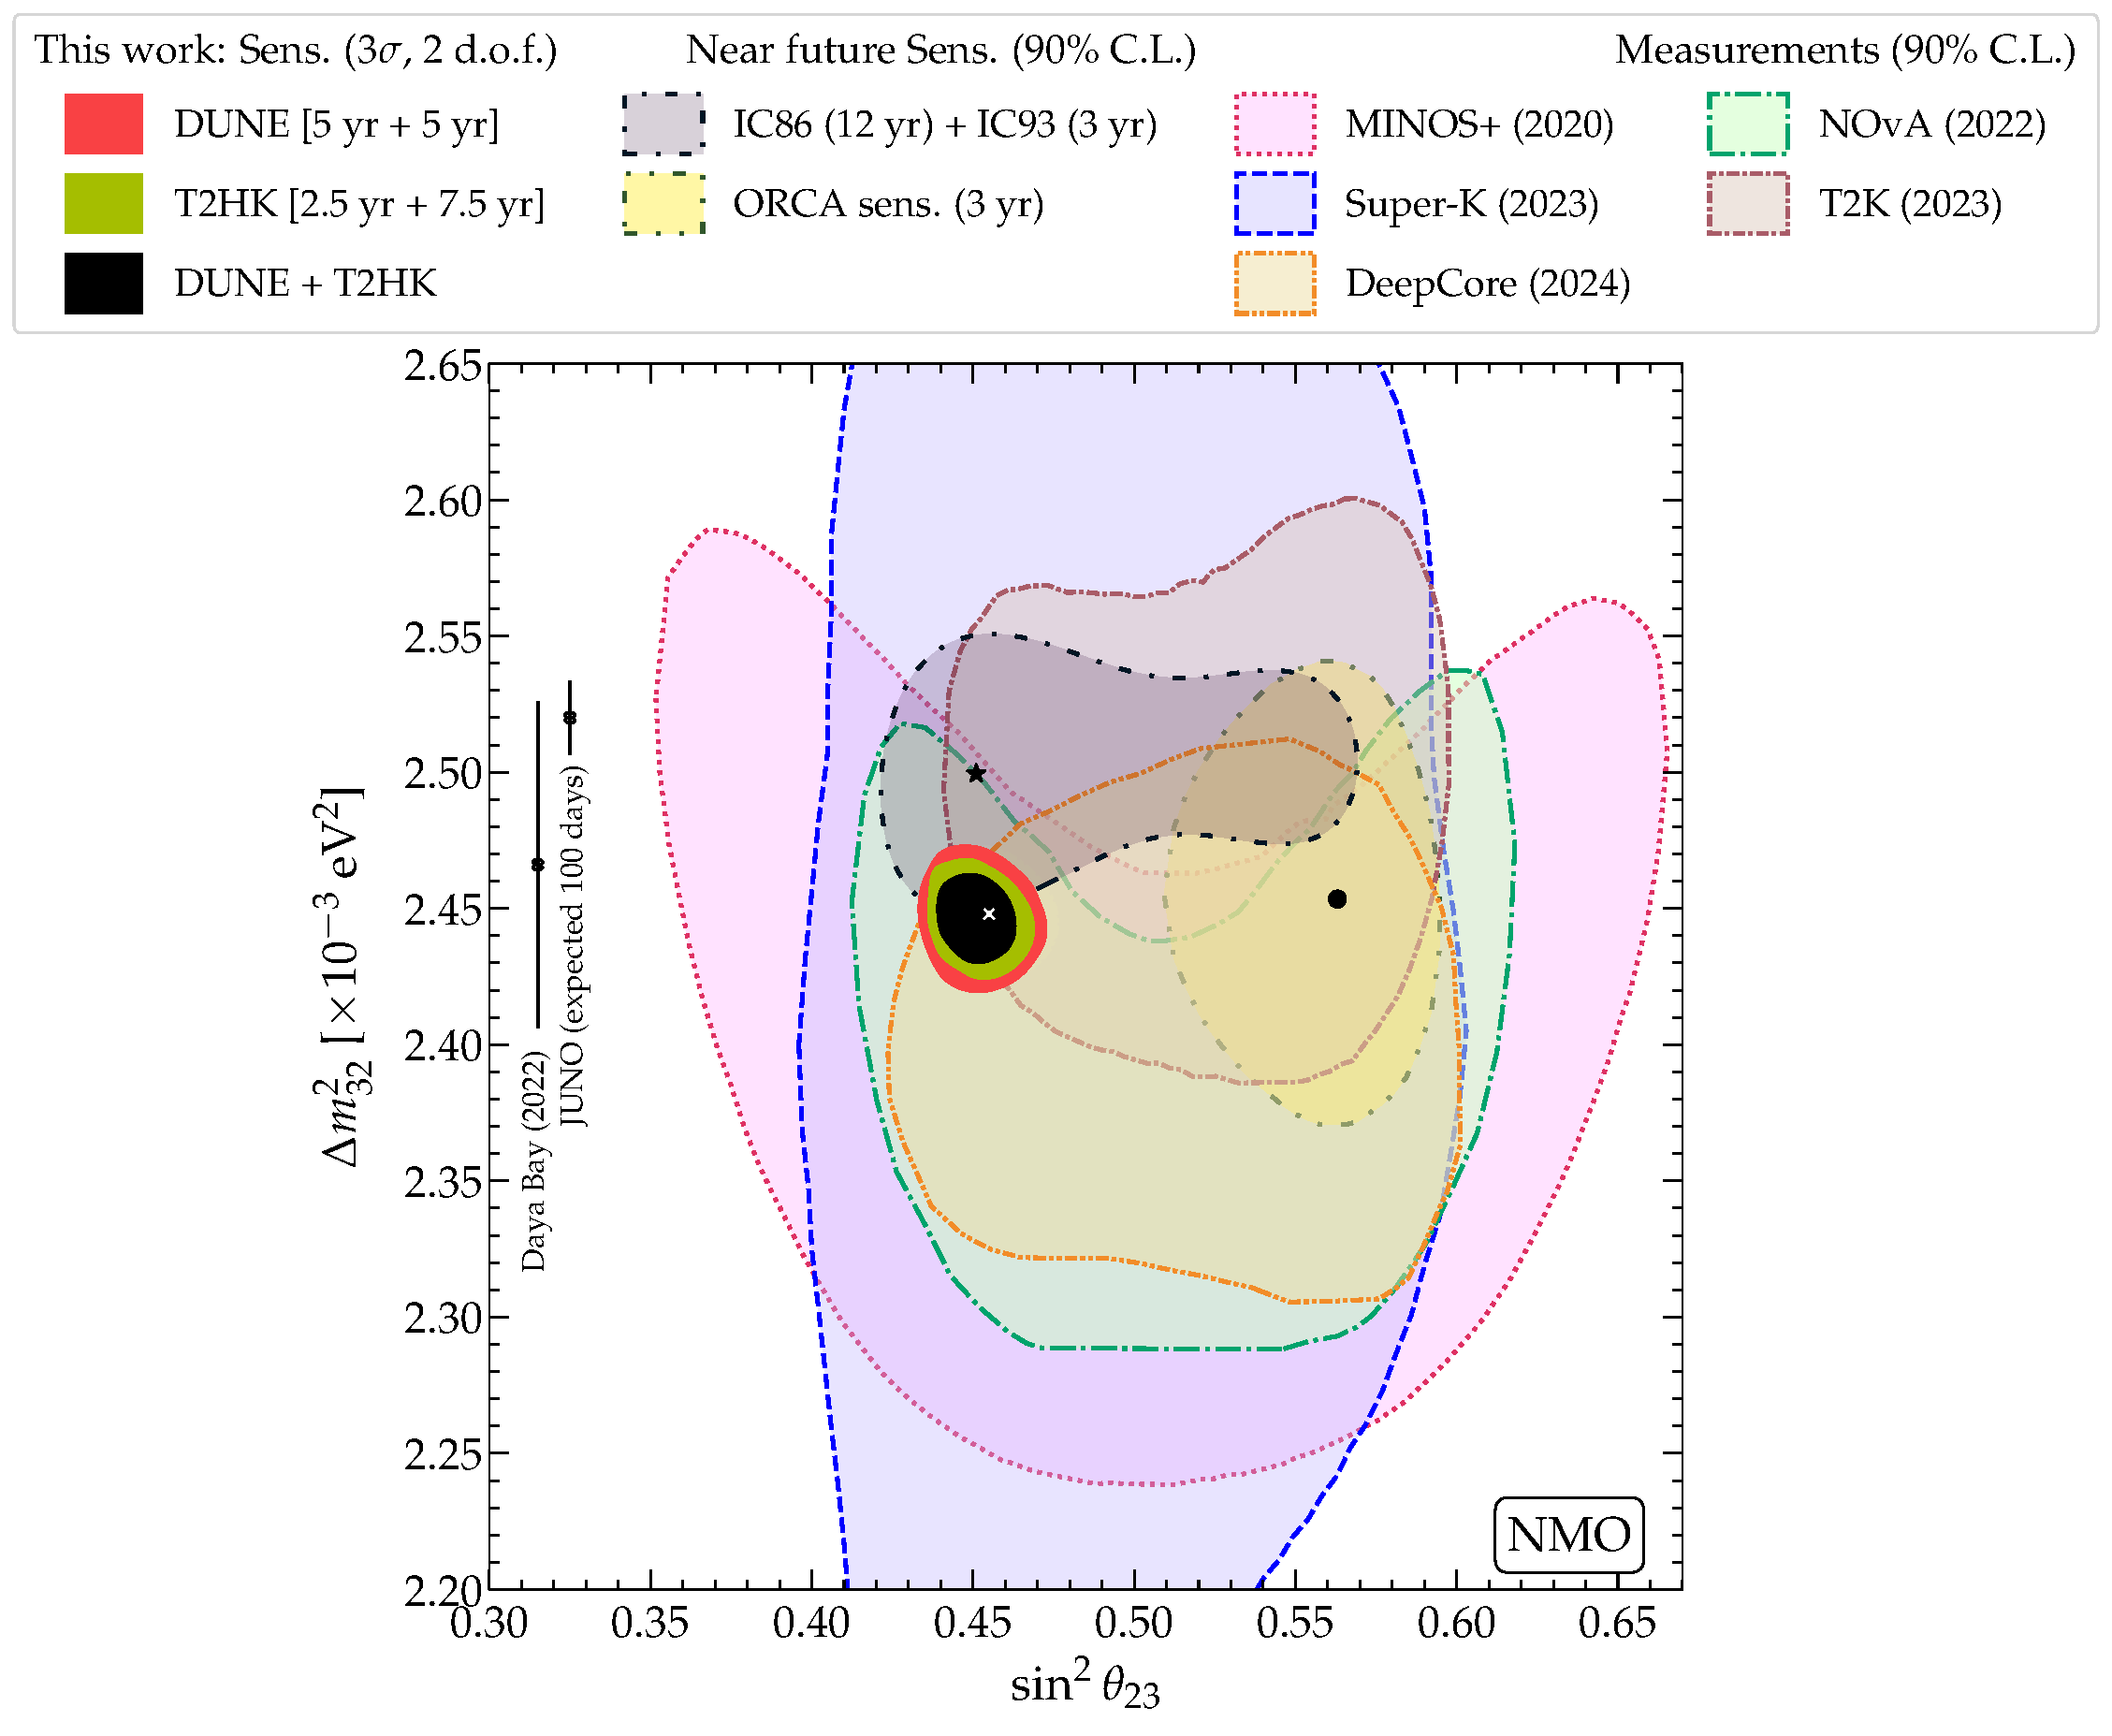
\includegraphics[width=\linewidth]{Figures/Chapter-5/th23_Dm31_Appen.pdf}
	\caption{\footnotesize{Allowed ranges at 3$\sigma$ (2 d.o.f.) in the atmospheric mixing parameters, $\sin^{2}\theta_{23}$ and $\Delta m^{2}_{32}$, using DUNE, T2HK, and DUNE + T2HK. DUNE is expected to have an exposure of 480 kt$\cdot$MW$\cdot$yr and T2HK, an exposure of 2431 kt$\cdot$MW$\cdot$yr. Same as figure~\ref{fig:moneyplot}, we show existing allowed ranges from: Super-K~\cite{linyan_wan_2022_6694761}, T2K~\cite{T2K:2023smv}, NO$\nu$A~\cite{NOvA:2021nfi}, MINOS~\cite{MINOS:2020llm}, and IceCube DeepCore~\cite{IceCube:2024xjj}. We also show existing (expected) bounds on $\Delta m^{2}_{32}$ from Daya Bay~\cite{DayaBay:2022orm} JUNO ~\cite{JUNO:2022mxj}). Additionally, we also show expected sensitivity from IceCube Deepcore (12 yr) + Upgrade (3 yr)~\cite{IceCube:2023ins}, and ORCA (3 yr)~\cite{KM3NeT:2021ozk}. Refer to the text for details.}}
	\label{fig:appendix-allowed-ranges-nmo}
\end{figure}
%---------------------------------------------------------------

In addition to the details in table~\ref{table:one}, in figure~\ref{fig:appendix-allowed-ranges-nmo}, we also show the expected allowed ranges using the near future development in the two giant atmospheric experiments: IceCube DeepCore and KM3NeT/ORCA. In ref.~\cite{IceCube:2023ins}, the expected sensitivity in atmospheric parameters is studied for 12 years of IceCube with 86 strings along with extra seven strings of IceCube Upgrade from 2026 onwards for three years. Strong improvements can be observed with the expected Upgrade in IceCube DeepCore. In ref.~\cite{KM3NeT:2021ozk}, the expected sensitivity of KM3NeT/ORCA after three years of data taking is studied, which we show in figure~\ref{fig:appendix-allowed-ranges-nmo}. The present scenario hints that the ongoing experiments in the near future will be able to obtain further precision on the $(\Delta m^2_{32} - \sin^{2}\theta_{23})$ plane. For comparison, we also show the assumed best-fit values by the two experiments: IceCube Upgrade ($\sin^{2}\theta_{23} = 0.451, \, \Delta m^2_{32} = 2.49 \times 10^{-3}$ eV$^{2}$) and ORCA ($\sin^{2}\theta_{23} = 0.563, \, \Delta m^2_{32} = 2.45 \times 10^{-3}$ eV$^{2}$). It should be noted that since their benchmark value for $\sin^{2}\theta_{23}$ corresponds to the opposite octant, the allowed region they expect seems complementary. 

%===========================================================================



%%%%%%%%%%%%%%%%%%%%%%%%%%%%%%%%%%%%%%%%%%
\section{Summary and conclusions}
\label{conclusion}
%%%%%%%%%%%%%%%%%%%%%%%%%%%%%%%%%%%%%%%%%%
The present generation of neutrino experiments have undoubtedly paved the way for precision studies in neutrino physics. The reactor mixing angle ($\theta_{13}$) measured by Daya Bay has achieved a remarkable precision of 2.8\%~\cite{DayaBay:2022orm}. Solar parameters: $\theta_{12}$ and $\Delta m^{2}_{21}$ have long been measured and stand presently with a relative 1$\sigma$ error of 4.5\% and 2.3\%\,, respectively from the global fit~\cite{Capozzi:2021fjo}. The most precisely measured oscillation parameter is, ironically, the magnitude of atmospheric mass-squared difference ($\Delta m^{2}_{31}$), while determining its sign still remains one of the big questions in neutrino physics left unanswered. The two most uncertain parameters are the atmospheric mixing angle, $\theta_{23}$, and Dirac CP phase, $\delta_{\mathrm{CP}}$. 

In this work, we address the issue of maximal mixing solution of $\sin^{2}\theta_{23}$ and if non-maximal, then ruling out the wrong octant solutions of $\sin^{2}\theta_{23}$. We also study the achievable precision on $(\sin^{2}\theta_{23}-\delta_{\mathrm{CP}})$ and $(\sin^{2}\theta_{23}-\Delta m^{2}_{31})$ planes. To analyze the mentioned issues, we compare and contrast the standalone DUNE and T2HK with their complementarities in the combined DUNE + T2HK setup. While DUNE and T2HK, individually, should be able to improve on the sensitivity studies of deviation from maximal $\sin^{2}\theta_{23}$, exclusion of its wrong octant solutions, and precision measurements, their individual sensitivities are hampered by degeneracies due to uncertainties in $\sin^{2}\theta_{23}$, $\delta_{\mathrm{CP}}$, and $\Delta m^{2}_{31}$.  However, DUNE and T2HK have complementary capabilities: while T2HK is especially well-suited to measure $\sin^{2}\theta_{23}$ and $\delta_{\mathrm{CP}}$, DUNE is especially well-equipped to measure $\Delta m^{2}_{31}$. Thus, combining DUNE and T2HK brings many novelties.
 
We find that the combined DUNE + T2HK increases the sensitivity to establish a deviation from maximality to $\sim 8\sigma$ if in Nature, $\sin^{2}\theta_{23}$ is same as the benchmark value mentioned in table~\ref{table:one}, following present global fit in ref.~\cite{Capozzi:2021fjo}. However, if this present best-fit shifts to its present $1\sigma$ allowed upper bound ($\sim 0.473$), then the combination is the only solution to achieve sensitivity to deviation from maximality greater than 3$\sigma$. The study of sensitivity towards deviation from maximal $\sin^{2}\theta_{23}$ as a function of exposure reveals that following the benchmark values, the discovery potential that combined DUNE + T2HK can reach with just 0.5 times the nominal exposure, is unattainable by either DUNE or T2HK even with their full exposures. In analyzing the sensitivity towards excluding incorrect octant solutions of $\sin^{2}\theta_{23}$, we find that the synergy of combined experiments significantly outperforms individual ones. While no single experiment achieves 5$\sigma$, the combination reaches approximately 8$\sigma$, assuming the true value of $\sin^{2}\theta_{23}$ is the same as the benchmark. Yet again, the discovery potential that standalone experiments attain with full exposure in eliminating the wrong octant, can be achieved by combining with just 0.4 times the full exposure. The estimated precision by alone DUNE and T2HK in both atmospheric parameters: $\sin^{2}\theta_{23}$ and $\Delta m^{2}_{31}$ improves present global fit precision by an approximate factor of 5 and 4, respectively. Furthermore, we find that the range of 5$\sigma$ precision that the combined DUNE + T2HK can achieve with only 0.25 times the exposure in $\Delta m^{2}_{31}$ is a level of precision that individual experiments cannot reach even with full exposures. Moreover, while studying the allowed ranges in $(\sin^{2}\theta_{23}- \delta_{\mathrm{CP}})$ plane, we notice that the weak hint towards clone solutions shown by standalone experiments at 3$\sigma$ can be resolved by the combination with just half the exposure.

Therefore, this study brings about novel perspectives of the upcoming high-precision LBL experiments DUNE and T2HK, stressing how their combination and 
hence, the possible complementarities among them may alleviate the need of a very high exposure from these individual experiments in obtaining the desired
sensitivities towards different oscillation parameters.

% \blankpage 
%%%%%%%%%%%%%%%%%%%%%%%%% Chapter-6 %%%%%%%%%%%%%%%%%%%%%%%%%%%%%%%
%%%%%%%%%%%%%%%%%%%%%%% CHAPTER - 6 %%%%%%%%%%%%%%%%%%%%
\chapter{Universality in Space-Time $\omega$ Modes of Quarkyonic Star }
\label{C6} 
%%%%%%%%%%%%%%%%%%%%%%%%%%%%%%%%%%%%%%%%%%%%%%%%%%%%%%%%%%
\subsection{Introduction}
\subsection{Results and Discussions}
\subsection{Conclusion}

%\blankpage 
%%%%%%%%%%%%%%%%%%%%%%%%% Chapter-7 %%%%%%%%%%%%%%%%%%%%%%%%%%%%%%%
%%%%%%%%%%%%%%%%%%%%%%%%% CHAPTER - 7 %%%%%%%%%%%%%%%%%%%%%%%%%
\chapter{Summary and Conclusions}
\label{C7}
%%%%%%%%%%%%%%%%%%%%%%%%%%%%%%%%%%%%%%%%%%%%%%%%%%%%%%%%%%%%%%%
\par This thesis addresses some important issues in three-flavor neutrino oscillation in the context of upcoming high-precision long-baseline experiments. Neutrinos are omnipresent and they are the second most abundant particles in the Universe after photons. There are a variety of neutrino sources (both natural and artificial) producing neutrinos over a wide range of energies in the range of $10^{-4}$ to $10^{18}$ eV or so and traveling distances from a few meters to hundreds of Gpc. Neutrinos were postulated first by Wolfgang Pauli in 1930 to explain how beta-decay could conserve energy, momentum, and angular momentum. In 1934, Enrico Fermi named the new particle as ``neutrino", which means the ``little neutral one" in the Italian language. In 1956, Clyde L. Cowan and Frederick Reines first observed neutrinos in a nuclear reactor. There are three (3) light active flavor neutrinos: $\nu_e$, $\nu_\mu$, and $\nu_\tau$ - experimentally confirmed by the precision data on the \textit{Z}-decay width at the $e^+e^-$ collider at LEP \cite{ALEPH:2005ab}. They only take part in weak interactions through massive \textit{W}$^\pm$ and \textit{Z}$^0$ gauge bosons. They are electrically neutral, left-handed, and form \textit{SU}$(2)$ doublets in the Standard Model with the corresponding left-handed charged leptons. In the basic SM of particle physics, neutrinos are massless due to the absence of right-handed neutrinos. \\
\par Over the past two decades, data from several world-class neutrino experiments firmly established that neutrinos change flavor after propagating a finite distance in space and time - a phenomenon known as ``neutrino oscillation". Neutrino oscillation demands non-zero neutrino mass and mixing. Hence, non-zero neutrino mass is the first experimental proof for physics beyond the Standard Model for which the Nobel Prize was awarded to Takaaki Kajita and Arthur McDonald in 2015. Neutrino oscillation, in the $3\nu$ paradigm, is mainly governed by six oscillation parameters, viz., solar mixing angle ($\theta_{12}$), atmospheric mixing angle ($\theta_{23}$), reactor mixing angle ($\theta_{13}$), Dirac CP-violating phase ($\delta_{\mathrm{CP}}$), solar mass-squared splitting ($\Delta m^2_{21} \equiv m^2_{2}-m^2_{1}$), and atmospheric mass-squared splitting ($\Delta m^2_{31} \equiv m^2_{3}-m^2_{1}$). Still, there are a few fundamental issues that need to be resolved in neutrino oscillation experiments, namely, i) the neutrino mass ordering (whether $\Delta m^2_{31}>0$, known as normal mass ordering - NMO, or $\Delta m^2_{31}<0$, termed as inverted mass ordering - IMO), ii) the octant of $\theta_{23}$ (whether $\theta_{23}<45^\circ$ known as lower octant - LO, or $\theta_{23}>45^\circ$ termed as higher octant - HO), and iii) whether the CP is violated in the neutrino sector like quark sector and if so, then what is the precise value of the CP phase? The next-generation high-precision long-baseline (LBL) experiments are capable to address these issues at a high confidence level. \\\vspace{0.1cm}
In this thesis, we study i) the physics reach of the upcoming LBL experiment, Deep Underground Neutrino Experiment (DUNE) in the US, to establish the possible deviation from maximal mixing of $\theta_{23}$, ii) to achieve an improved precision on the 2-3 oscillation parameters using the synergy between the DUNE and Tokai-to-Hyper-Kamiokande (T2HK) experiments, and iii) the possible impact of the flavor-dependent long-range neutrino interactions on the measurements of neutrino oscillation parameters in DUNE and T2HK.\\
\section{Establishing the deviation from maximal mixing of $\theta_{23}$ in DUNE:}\hspace{0.2cm}The robustness of the three-flavor neutrino oscillation paradigm got established on a strong footing after the discovery of non-zero $\theta_{13}$ in the Daya Bay experiment and opened the door for searching CP violation in currently running and upcoming LBL experiments. The recent global fit studies ~\cite{Capozzi:2021fjo,deSalas:2020pgw,Esteban:2020cvm,NuFIT} of the three-flavor neutrino oscillation parameters indicate that $\sin^2\theta_{23}\neq0.5$ or $\sin^22\theta_{23}\neq1$. This gives rise to the issue of non-maximal $\theta_{23}$, which is quite important from the neutrino mass-mixing models point of view. In this work, we study the prospect of the next-generation long-baseline (LBL) experiment DUNE to establish the non-maximal $\theta_{23}$ in light of the current neutrino oscillation data.\\
DUNE \cite{DUNE:2020jqi} is an upcoming LBL experiment with a baseline of 1285 km where neutrinos travel from Fermilab to Homestake Mine in South Dakota. It will use an on-axis, wide-band neutrino beam with high intensity covering both first and second oscillation maxima. Some of its notable features are the excellent energy resolution of the Liquid Argon TPC (LArTPC) having 40 kt fiducial volume, large matter effect due to a longer baseline, and less systematic uncertainties in the appearance channel. The neutrino flux peaks around the first oscillation maxima which occurs at 2.5 GeV for 1285 km.\\ 
The study of non-maximal $\theta_{23}$ is mostly driven by the disappearance channel, and hence the uncertainty in $\delta_{\mathrm{CP}}$ does not affect our results much. As the disappearance channel is statistics-driven, it also helps to improve the precision on $\theta_{23}$. Our benchmark choices of the oscillation parameters are from Capozzi $et$ al. \cite{Capozzi:2021fjo}, where we have only considered the NMO as the true mass ordering in Nature. In our benchmark choices, $\sin^2\theta_{23} = 0.455$ (in LO), and $\delta_{\mathrm{CP}} = 223^\circ$ (belongs to lower-half-plane). We fix the value of $\theta_{12},\, \theta_{13}$, and $\Delta m^2_{21}$ as they are already measured with high precision using solar and reactor experiments. In our analysis, we have allowed the values of $\theta_{23}, \Delta m^2_{31}$, and $\delta_{\mathrm{CP}}$ to vary within their $3\sigma$ allowed range as mentioned in \cite{Capozzi:2021fjo}.\\
As the disappearance probability $\propto$ $\sin^22\theta_{23}$, degeneracies persist at the total event level. However, due to the superior energy resolution of DUNE, this degeneracy can be lifted using spectral information alongwith the total event rates. Some energy bins around the 1st oscillation maxima ($i.e.$, at 2.5 GeV) show the maximum sensitivity towards the non-maximal $\theta_{23}$ whereas, the performance of lower and higher energy bins deteriorates for the benchmark value of $\Delta m^2_{31}$. We show, with [3.5 yr $\nu$ + 3.5 yr $\bar{\nu}$] run, DUNE can establish non-maximal $\theta_{23}$ at $\sim$ $5\sigma$ C.L. with total rate + shape analyses whereas, it gets dropped to $1.5\sigma$ C.L. with an analysis based on only total event rates.\\
\par We see that with 7 years of run time equally shared by neutrino and antineutrino, DUNE can establish non-maximal $\theta_{23}$ with $\sim$ 4.2$\sigma$ C.L. at the benchmark choice of true $\sin^2\theta_{23}$. It is obvious that the more the true (benchmark) value of $\sin^2\theta_{23}$ shifts towards the maximal mixing value, the more it will be difficult to establish non-maximality of $\theta_{23}$. It is noteworthy to mention that if the true value of $\sin^2\theta_{23}$ shifts towards the upper range of the $1\sigma$ uncertainty of $\sin^2\theta_{23}$ ($i.e.$, maximum limit within $1\sigma$ tolerance in the vicinity of MM), DUNE can still establish non-maximality of $\sin^2\theta_{23}$ with $\sim 2.1\sigma$ C.L. However, this study is improved for the enhanced run time [$i.e.$, 5 yr $\nu$ + 5 yr $\bar{\nu}$] as it is mainly governed by the statistics. We observe that a $3\sigma\, (5\sigma)$ determination of non-maximal $\theta_{23}$ is possible in DUNE with an exposure of 336 kt$\cdot$MW$\cdot$years if true $\sin^2\theta_{23}\lesssim 0.465\, (0.450)$ or $\sin^2\theta_{23}\gtrsim0.554\, (0.572)$ for any value of true $\delta_{\mathrm{CP}}$ in its present $3\sigma$ range and true NMO.\\
\section{Improved precision on the 2-3 oscillation parameters using the synergy between DUNE and T2HK:} \hspace{0.2cm} A high-precision measurement of $\Delta m^2_{31}$ and $\theta_{23}$ is inevitable to estimate the Earth's matter effect in long-baseline experiments which in turn plays an important role in addressing the issue of neutrino mass ordering and to measure the value of CP phase in $3\nu$ framework. Following the footprints of present-generation measurements and near-future sensitivities from different oscillation experiments, our work examines how next-generation experiments, DUNE and T2HK, bring improvement in the 2-3 sector which will also help to decipher the long-standing flavor problem glorifying the oscillation-based neutrino research in the precision era. We highlight the relevance of the complementarity between DUNE and T2HK in determining the sensitivity towards deviation from maximal $\theta_{23}$, excluding the wrong octant of $\theta_{23}$, and establishing the precision on atmospheric parameters.\\
\par The next-generation long baseline experiment in Japan, T2HK, \cite{Hyper-KamiokandeProto-:2015xww, Hyper-Kamiokande:2018ofw} will use an off-axis, narrow-band neutrino beam that will travel through a distance of 295 km from J-PARC to Hyper-Kamiokande. This experiment has several features that are complementary to DUNE. Due to its short baseline, T2HK will experience less matter effect than DUNE and can have better prospects in measuring intrinsic CP violation due to $\delta_{\mathrm{CP}}$. T2HK's larger detector volume than DUNE can improve any disappearance-driven phenomena with the power of more enriched statistics. To compensate for the low antineutrino cross section, T2HK has been planned with 3 times higher run time in antineutrino mode than neutrino [2.5 yr $\nu$ + 7.5 yr $\bar{\nu}$]. T2HK's larger systematic uncertainty in appearance channel ($5\%$) than DUNE ($2\%$) is responsible for reduced sensitivity in any analysis driven by appearance channel, whereas, its improved disappearance systematics ($3.5\%$) than DUNE ($5\%$) along with larger detector volume helps to improve any disappearance-driven sensitivity.\\
We show that T2HK, with its benchmark exposure of 2431 kt$\cdot$MW$\cdot$yr, can establish non-maximal $\theta_{23}$ at $5.6\sigma$ C.L. which deteriorates a bit for DUNE to $5\sigma$ with its benchmark exposure of 480 kt$\cdot$MW$\cdot$yr at the benchmark choice of $\sin^2\theta_{23}$ ($i.e.$, 0.455) \cite{Capozzi:2021fjo} assuming NMO. T2HK's enriched statistics and less systematic uncertainty in the disappearance channel enhance its performance over DUNE. The performance is much improved ($\sim 7.6\sigma$) in the combined setup of DUNE + T2HK as compared to their standalone setups. The notable finding is that, in Nature, if true $\sin^2\theta_{23}$ attains the upper boundary of the current $1\sigma$ uncertainty (0.473) which is close to MM, only DUNE + T2HK can achieve $3\sigma$ sensitivity of non-maximal $\theta_{23}$ with the present best-fit values of oscillation parameters. Based on the current benchmark choices of oscillation parameters \cite{Capozzi:2021fjo}, the range of true values of $\sin^{2}\theta_{23}$ that can be differentiated from MM choices, by DUNE + T2HK with just half of their nominal exposures, cannot be achieved by either of the individual experiments even with their respective full projected exposures.\\
We study one of the most pressing unsolved issues in $3\nu$ paradigm, $i.e.$, the octant ambiguity of $\theta_{23}$. As it is driven by appearance channel, DUNE performs better ($5.2\sigma$) in excluding the wrong octant solution of $\theta_{23}$ with its nominal exposure than T2HK ($4.4\sigma$) at benchmark value of $\sin^2\theta_{23} = 0.455$ for true $\delta_{\mathrm{CP}} = 223^\circ$ and true NMO. However, the joint setup of DUNE + T2HK outperforms ($7.4\sigma$) in our study than their solo performances. Here also, our finding show that the joint performance of DUNE + T2HK can give $\sim 4\sigma$ sensitivity to our study at the upper edge of $1\sigma$ uncertainty in $\sin^2\theta_{23}$ ($i.e.$, in the vicinity of MM). At lower confidence, T2HK wins due to larger statistics, whereas, at higher confidence, DUNE wins due to lesser systematics in the appearance channel. One more noteworthy finding in this context is that, with just 0.25 times the benchmark exposure of the individual experiments, the combined setup can exclude $60\%$ of $\theta_{23}$ from the wrong octant solutions at $3\sigma$ C.L.\\
\par We address one more pertinent issue in the precision domain of neutrino oscillation, viz., precision measurements of $\sin^2\theta_{23}$ and $\Delta m^2_{31}$ around their benchmark choices ($i.e.$, 0.455 and $2.522\times10^{-3}$ eV$^2$) for NMO. Due to the statistical abundance, the standalone T2HK shows more precise measurements than DUNE and, of course, their combined setup enhances the performance in these measurements than their individual setups at their nominal exposures. The highlighted result from this section is that, the combined setup improves the present achievable precision of $\sin^2\theta_{23}$ and $\Delta m^2_{31}$, by a factor of 7 and 5, respectively. While standalone DUNE and T2HK with low exposures ($\sim 0.25$ times nominal exposure) cannot rule out clone solutions in $\sin^2\theta_{23}$ at $3\sigma$, the combined DUNE + T2HK provide degeneracy-free measurements. In the case of $\Delta m^2_{31}$, using approximately $20\%$ of the individual exposures of DUNE and T2HK together can achieve an impressive relative $1\sigma$ precision of $0.25\%$.\\
The combination of DUNE and T2HK can exclude the HO only in antineutrino
mode at $3\sigma$ C.L. breaking $(\sin^2\theta_{23} - \delta_{\mathrm{CP}})$ degeneracy due to higher $\bar{\nu}$ statistics in T2HK. So, the majority of the appearance events are free from fake (matter-induced) CP-phase. However, for the combined neutrino and antineutrino modes, we can give more precise measurements of $\sin^2\theta_{23}$ and $\Delta m^2_{31}$ by squeezing the parameter space irrespective of all experimental setups under discussion. DUNE's excellent energy-resolution helps to precisely measure $\Delta m^2_{31}$ whereas, T2HK's statistical enrichment assists to precisely measure $\sin^2\theta_{23}$. We also show the reduction in the parameter space $(\sin^2\theta_{23} - \delta_{\mathrm{CP}})$ using DUNE and T2HK, either in isolation or in combination. We find that, at half-exposure, the synergy between DUNE and T2HK is the only hope to exclude the MM solution and disfavor the CP-conserving region.\\
\section{Impact of long-range neutrino interactions on the measurements of oscillation parameters at DUNE and T2HK :} \hspace{0.2cm} Neutrino oscillation, having the bright prospect of measuring oscillation parameters with high precision in the next-generation experiments, may unravel novel signatures of BSM physics. The symmetries of the Standard Model are preserved under the gauge group \textit{SU}$(3)_C\,\otimes\,$\textit{SU}$(2)_L\,\otimes\,$\textit{U}$(1)_Y$. Now, a new, anomaly-free interaction can be added through a simple extension of the gauge group, viz., \textit{U}$(1)^\prime$, which brings some new symmetries in the Standard Model. These symmetries are chosen as the difference between the lepton numbers, $i.e.$, $(L_e-L_\mu)$, $(L_e-L_\tau)$, and $(L_\mu-L_\tau)$, manifesting the new interactions in Nature. Now, if the mass of the corresponding gauge boson $Z^\prime$ is very light ($\leq\,10^{-10}$ eV), the new interaction is long-ranged and characterized as a long-range interaction (LRI). The next-generation LBL experiments DUNE and Hyper-K may feel the presence of these new interactions \cite{Singh:2023nek}. In this work, we showcase the prominent effect of LRI along with the standard neutrino interaction (SI) in DUNE, T2HK, and their combined setups on measuring non-maximal $\theta_{23}$ and leptonic CP violation. The value of $(\Delta m^2_{31}/2E)$ for DUNE at 1st oscillation maxima is $\sim$ $10^{-13}$ eV which is compatible with the order of magnitude of LRI potential and hence DUNE and T2HK are good portals in probing the existence of LRI potential through oscillation. We assume NMO as a true mass ordering in Nature and the true LRI potential as $1.4\times10^{-14}$ eV, $1.0\times10^{-14}$ eV, and $0.73\times10^{-14}$ eV for $(L_e-L_\mu)$, $(L_e-L_\tau)$, and $(L_\mu-L_\tau)$ symmetries, respectively \cite{Singh:2023nek} throughout our analyses. In general, $L_e-L_\mu$ and $L_e-L_\tau$ are sensitive to $\delta_{\mathrm{CP}}$ and $\theta_{23}$ whereas, 
$L_\mu-L_\tau$ symmetry is  more sensitive to $\Delta m^2_{31}$ and $\theta_{23}$.\\
When the strength of long-range interactions increases ($V_{\rm{LRI}} > 10^{-14}$ eV), the distinguishable fraction of $\sin^{2}\theta_{23}$ values in Nature, deviating from maximal mixing, increases significantly. This enhancement is more pronounced under the $L_{\mu} - L_{\tau}$ symmetry, where the combined capabilities of DUNE and T2HK can achieve a coverage of approximately 90\% if $V_{\mu\tau}\,(\mathrm{true}\sim5\times10^{-14})$ eV. This improvement is attributed to the substantial disappearance event statistics in both DUNE and T2HK. For an illustrative true LRI value of $\sim 10^{-14}$ eV, we find that if the true octant of $\sin^{2}\theta_{23}$ in Nature corresponds to the lower octant (LO), the presence of LRI interactions under all the three symmetries reduces the sensitivity to deviations from maximal mixing compared to the SI scenario. Conversely, the sensitivity improves when $\sin^{2}\theta_{23}$ resides in the higher octant (HO) and is close to maximal mixing. We observe similar findings when studying the sensitivity towards the exclusion of the wrong octant. $L_{\mu} - L_{\tau}$ symmetry affects the most. We also investigate the impact of subdominant LRI on establishing leptonic CP violation (CPV). Our analysis reveals that if subdominant LRI exists in Nature, the fraction of $\delta_{\rm{CP}}$ values capable of establishing CPV at $\geq 3\sigma$ under each symmetry decreases significantly. This reduction arises from the critical role of $\sin^{2}2\theta_{13}$ evolution as a function of neutrino energy in the presence of matter. For an illustrative value of $V_{\rm{LRI}} \sim 10^{-14}$ eV, we find that the presence of LRI has a relatively greater impact on CPV sensitivity in DUNE compared to T2HK. This can be attributed to the higher prevalence of fake CP asymmetry in DUNE due to its longer baseline. Additionally, the $L_\mu - L_\tau$ symmetry introduces the most significant degradation in CPV sensitivity. This deterioration is primarily driven by the degeneracy between $V_{\rm{LRI}}$ and the uncertainty in $\sin^{2}\theta_{23}$. We also analyze the impact of LRI on the allowed parameter ranges in $(\sin^2\theta_{23}-\delta_{\mathrm{CP}})$ plane and observe varying effects across different symmetries. Under the $L_{e}-L_{\tau}$ symmetry, the allowed ranges remain largely consistent with those under SI, as sensitivity in this case is predominantly driven by the appearance statistics. For the $L_{e}-L_{\mu}$ symmetry, a noticeable deterioration in the precision of $\sin^{2}\theta_{23}$ is observed in DUNE when the data is generated with $\sin^{2}\theta_{23}$ in the LO. However, the complementarity between DUNE and T2HK resolves these degeneracies, resulting in stringent allowed regions under LRI that are comparable to those in the SI scenario. To conclude, our findings emphasize that while subdominant LRIs may influence the sensitivity and precision measurements of oscillation parameters, the complementary capabilities of DUNE and T2HK mitigate these challenges to a large extent. This synergy underscores the importance of a combined experimental approach in disentangling the impact of LRIs from neutrino oscillation under SI.

%\blankpage 
%%%%%%%%%%%%%%%%%%%%%%%%%%%%%%%%%%%%%%%%%%%%%%%%%%%%%%%%%%%%%%%%%%%
%%%%%%%%%%%%%%%%%%%%%%%%% Appendix %%%%%%%%%%%%%%%%%%%%%%%%%%%%%%%
\appendix

% Force Appendix label to always be A internally
\renewcommand\thechapter{A}

% Numbering styles inside appendix
\renewcommand\thesection{\thechapter.\arabic{section}}
\renewcommand\theequation{\thechapter.\arabic{equation}}
\renewcommand\thefigure{\thechapter.\arabic{figure}}
\renewcommand\thetable{\thechapter.\arabic{table}}
\counterwithin{equation}{chapter}

% Suppress automatic "Appendix A" chapter title
\chapter*{Appendix}
\addcontentsline{toc}{chapter}{Appendix}

% Remove chapter number from page headers (if using fancyhdr)
\markboth{Appendix}{Appendix}

\setcounter{section}{0}
\setcounter{chapter}{1} % keeps counters sane internally

%%%%%%%%%%%%%%%%%%%%%%%%% CHAPTER - 7 %%%%%%%%%%%%%%%%%%%%%%%%%

%%%%%%%%%%%%%%%%%%%%%%%%%%%%%%%%%%%%%%%%%%%%%%%%%%%%%%%%%%%%%%%
\chapter{Phase Amplitude Method}
\label{app:running_osc_params}

\subsection{Phase amplitude method}
\label{Formalism4}

Equation (\ref{zerilli_eq}) bears a formal resemblance to the time-independent Schrödinger equation; obtaining accurate solutions for quasinormal mode frequencies is a highly non-trivial numerical undertaking. The primary challenge lies in the precise implementation of the physical boundary condition requiring purely outgoing gravitational waves at spatial infinity. This requirement must be translated into a numerical computation in two problematic steps: first, one must approximate ``infinity" by a finite but large radial coordinate, and second—constituting the major numerical difficulty—one must clearly separate two linearly independent solutions whose asymptotic behavior is exponentially growing and decaying, respectively. This numerical instability, where tiny errors in the decaying solution can be overwhelmed by contamination from the growing solution, has spawned the development of specialized techniques such as Leaver’s continued-fraction method and various WKB/phase-integral approximations \cite{leaver_QNM_techniques_1985,Kokkotas_living_review}.

In the present work, we employ the phase-amplitude method, as formulated by Anderson et al.~\cite{Anderson_inverse_cowling}. This method is originally developed and demonstrated in the calculation of black hole quasinormal modes. Its application to the neutron star problem is well-motivated, as it directly addresses the core numerical difficulty. The method's advantage is highlighted in comparative studies where traditional phase-integral approaches, such as the one derived by Fr\"oman et al.\cite{Fromen}, were found to yield reliable frequencies only for the very lowest-order modes. In contrast, the phase-amplitude method is shown to generate highly accurate normal-mode frequencies across a wide spectrum. It achieves this robustness by reformulating the problem in terms of a phase function and its derivative, which remain well-behaved numerically even where the wavefunction itself is not. This stability allows for a more precise determination of the complex eigenfrequencies that satisfy the outgoing-wave boundary condition. The following section provides a detailed description of the phase-amplitude formalism and its specific implementation for calculating the quasinormal modes of neutron stars. 
The phase-amplitude method, as introduced by Anderson et al.~\cite{Anderson_inverse_cowling}, provides a robust framework for overcoming the numerical challenges inherent in solving the Zerilli equation for quasinormal modes. The method begins with a transformation of the dependent variable designed to simplify the asymptotic behavior of the solutions. Specifically, one defines a new function \(\Psi\) related to the Zerilli function \(Z\) by:
\begin{equation}
	Z = \left(1 - \frac{2M}{r}\right)^{-1/2} \Psi.
\end{equation}
This transformation removes the first derivative term from the resulting wave equation, yielding a Schrödinger-like form:
\begin{equation}
	\left( \frac{d^2}{dr^2} + U(r) \right) \Psi = 0,
\end{equation}
where the effective potential \(U(r)\) incorporates the original Zerilli potential \(V_Z(r)\) along with additional terms arising from the coordinate transformation. The key insight is to express the two linearly independent solutions \(\Psi^\pm\) in a phase-amplitude form:
\begin{equation}
	\Psi^\pm = q^{-1/2} \exp\left[ \pm i \int^r q(\hat{r}) \, d\hat{r} \right],
\end{equation}
where the function \(q(r)\) satisfies the nonlinear differential equation\cite{Anderson_inverse_cowling}:
\begin{equation}
	\frac{1}{2q} \frac{d^2 q}{dr^2} - \frac{3}{4q^2} \left( \frac{dq}{dr} \right)^2 + q^2 - U = 0.
\end{equation}
Although this equation is nonlinear and appears more complex, it possesses significant numerical advantages. While the original wavefunction \(\Psi\) oscillates rapidly, especially for high frequencies, the function \(q(r)\) is typically slowly varying. This slow variation makes \(q(r)\) amenable to stable numerical integration. Initial conditions for \(q\) can be generated using the WKB approximation \(q \approx \sqrt{U}\) at a large distance from the star, where \(U\) varies slowly.

The phenomenon of Stokes lines plays a crucial role in understanding the behavior of the solutions and must be accounted before numerical integration \cite{Anderson_inverse_cowling}. Stokes lines are curves in the complex plane emanating from turning points (zeros of \(U\)) where the asymptotic behavior of the WKB solutions changes discontinuously. When crossing a Stokes line, the coefficient of the subdominant exponential solution can change abruptly—a phenomenon known as the Stokes phenomenon \cite{Anderson_inverse_cowling}. This means that a linear combination of \(\Psi^+\) and \(\Psi^-\) that represents the physical solution on one side of a Stokes line may not be valid on the other side. 

To handle this properly, one must identify the appropriate anti-Stokes lines in the complex \(r\)-plane. Anti-Stokes lines are curves along which the phase integral \(\int q \, dr\) is purely real, ensuring that the solutions remain oscillatory and bounded. For quasinormal modes with complex frequency \(\omega\), the optimal integration path is a straight line with slope given by \(\tan \theta = -\text{Im} \, \omega / \text{Re} \, \omega\), which aligns with an anti-Stokes line. This path choice is essential for suppressing the exponential divergence of the outgoing wave solution and obtaining numerically stable results. The derivative along this path is computed using:
\begin{equation}
	\frac{dq}{dr} = e^{-i\theta} \frac{dq}{d\rho},
\end{equation}
where \(\rho\) is the real distance along the integration path. The phase-amplitude method inherently accounts for the Stokes phenomenon by working with the slowly varying \(q\)-function, which remains smooth across Stokes lines, thereby avoiding the discontinuities that come from WKB approaches.

The numerical solution proceeds by integrating the \(q\)-equation from a large complex \(r\) (where the WKB initial conditions are valid) inward along the chosen anti-Stokes line to the stellar surface \(r = R\). At the surface, the exterior solution must match the interior solution. The matching condition leads to an expression for the amplitude ratio of incoming to outgoing waves. This ratio can be expressed as \cite{Anderson_inverse_cowling}:
\begin{equation}
	\mathcal{R}(\omega) = \frac{ 
		\mathcal{Z}_2 \left[ \left(1 - \frac{2M}{R} \right) \left( i q + \frac{1}{2q} \frac{dq}{dr} \right) + \frac{M}{R^2} \right] + \frac{d\mathcal{Z}_2}{dr}
	}{ 
		\mathcal{Z}_2 \left[ \left(1 - \frac{2M}{R} \right) \left( i q - \frac{1}{2q} \frac{dq}{dr} \right) - \frac{M}{R^2} \right] - \frac{d\mathcal{Z}_2}{dr}
	},
\end{equation}
where \(\mathcal{Z}_2\) represents the interior solution evaluated at the stellar surface, and all quantities are computed at \(r = R\). The quasinormal modes are precisely those complex frequencies \(\omega_n\) for which this ratio vanishes, \(\mathcal{R}(\omega_n) = 0\), indicating no incoming radiation. This condition is solved iteratively, and the use of the complex path along anti-Stokes lines ensures that the exponentially growing component is controlled, allowing for accurate determination of the mode frequencies. This approach has proven highly effective for both black hole and neutron star perturbations, providing reliable results even for highly damped modes where traditional WKB methods fail. 



%\blankpage 
%%%%%%%%%%%%%%%%%%%%%%%%%%%%%%%%%%%%%%%%%%%%%%%%%%%%%%%%%%%%%%%%%%%
\addcontentsline{toc}{chapter}{REFERENCES}
\bibliographystyle{hcdas}
\bibliography{thesis}
\end{document}
%%%%%%%%%%%%%%%%%%%%%%%%%%%%%%%%%%%%%%%%%%%% END %%%%%%%%%%%%%%%%%%%%%%%%%%%%%%%%%%%%%%%%
